\definecolor{mycolor1}{rgb}{0.00000,0.44700,0.74100}%
\definecolor{mycolor2}{rgb}{0.85000,0.32500,0.09800}%
\definecolor{mycolor3}{rgb}{0.92900,0.69400,0.12500}%
%
\begin{tikzpicture}

\begin{axis}[%
width=5cm,
height=4cm,
at={(0\linewidth,0\linewidth)},
scale only axis,
xmin=0,
xmax=320,
xlabel={Time [s]},
xmajorgrids,
ymin=1,
ymax=1.18,
ylabel={Tank Output Pressure [atm]},
ylabel style={yshift=-0.1cm},
ymajorgrids,
axis background/.style={fill=white},
% title style={font=\bfseries},
% title={Tank Output Pressure},
axis x line*=bottom,
axis y line*=left,
legend style={legend cell align=left,align=left,draw=white!15!black}
]
% This file was created by matlab2tikz.
%
\definecolor{mycolor1}{rgb}{0.00000,0.44700,0.74100}%
\definecolor{mycolor2}{rgb}{0.85000,0.32500,0.09800}%
\definecolor{mycolor3}{rgb}{0.92900,0.69400,0.12500}%
%
\begin{tikzpicture}

\begin{axis}[%
width=5cm,
height=4cm,
at={(0\linewidth,0\linewidth)},
scale only axis,
xmin=0,
xmax=320,
xlabel={Time [s]},
xmajorgrids,
ymin=1,
ymax=1.18,
ylabel={Pressure [atm]},
ymajorgrids,
axis background/.style={fill=white},
% title style={font=\bfseries},
% title={Tank Output Pressure},
axis x line*=bottom,
axis y line*=left,
legend style={legend cell align=left,align=left,draw=white!15!black}
]
\addplot [color=mycolor1,solid,line width=1.5pt]
  table[row sep=crcr]{%
0	1.03\\
0.25	1.03084\\
0.5	1.03105\\
0.75	1.03093\\
1	1.03093\\
1.25	1.03094\\
1.5	1.03091\\
1.75	1.03087\\
2	1.03084\\
2.25	1.03081\\
2.5	1.03079\\
2.75	1.03076\\
3	1.03074\\
3.25	1.03072\\
3.5	1.0307\\
3.75	1.03068\\
4	1.03066\\
4.25	1.03064\\
4.5	1.03062\\
4.75	1.03061\\
5	1.03059\\
5.25	1.03058\\
5.5	1.03057\\
5.75	1.03055\\
6	1.03054\\
6.25	1.03053\\
6.5	1.03052\\
6.75	1.03051\\
7	1.03051\\
7.25	1.0305\\
7.5	1.03049\\
7.75	1.03048\\
8	1.03048\\
8.25	1.03047\\
8.5	1.03046\\
8.75	1.03046\\
9	1.03045\\
9.25	1.03045\\
9.5	1.03045\\
9.75	1.03044\\
10	1.03044\\
10.25	1.03043\\
10.5	1.03043\\
10.75	1.03043\\
11	1.03043\\
11.25	1.03042\\
11.5	1.03042\\
11.75	1.03042\\
12	1.03042\\
12.25	1.03042\\
12.5	1.03042\\
12.75	1.03042\\
13	1.03042\\
13.25	1.03042\\
13.5	1.03042\\
13.75	1.03041\\
14	1.03042\\
14.25	1.03042\\
14.5	1.03042\\
14.75	1.03042\\
15	1.03042\\
15.25	1.03042\\
15.5	1.03042\\
15.75	1.03042\\
16	1.03042\\
16.25	1.03042\\
16.5	1.03042\\
16.75	1.03042\\
17	1.03043\\
17.25	1.03043\\
17.5	1.03043\\
17.75	1.03043\\
18	1.03043\\
18.25	1.03043\\
18.5	1.03044\\
18.75	1.03044\\
19	1.03044\\
19.25	1.03044\\
19.5	1.03045\\
19.75	1.03045\\
20	1.03045\\
20.25	1.03045\\
20.5	1.03046\\
20.75	1.03046\\
21	1.03046\\
21.25	1.03046\\
21.5	1.03047\\
21.75	1.03047\\
22	1.03047\\
22.25	1.03047\\
22.5	1.03048\\
22.75	1.03048\\
23	1.03048\\
23.25	1.03049\\
23.5	1.03049\\
23.75	1.03049\\
24	1.03049\\
24.25	1.0305\\
24.5	1.0305\\
24.75	1.0305\\
25	1.0305\\
25.25	1.03051\\
25.5	1.03051\\
25.75	1.03051\\
26	1.03051\\
26.25	1.03052\\
26.5	1.03052\\
26.75	1.03052\\
27	1.03052\\
27.25	1.03053\\
27.5	1.03053\\
27.75	1.03053\\
28	1.03053\\
28.25	1.03054\\
28.5	1.03054\\
28.75	1.03054\\
29	1.03054\\
29.25	1.03054\\
29.5	1.03055\\
29.75	1.03055\\
30	1.03055\\
30.25	1.03055\\
30.5	1.03055\\
30.75	1.03056\\
31	1.03056\\
31.25	1.03056\\
31.5	1.03056\\
31.75	1.03056\\
32	1.03057\\
32.25	1.03057\\
32.5	1.03057\\
32.75	1.03057\\
33	1.03057\\
33.25	1.03057\\
33.5	1.03057\\
33.75	1.03057\\
34	1.03058\\
34.25	1.03058\\
34.5	1.03058\\
34.75	1.03058\\
35	1.03058\\
35.25	1.03058\\
35.5	1.03058\\
35.75	1.03058\\
36	1.03058\\
36.25	1.03059\\
36.5	1.03059\\
36.75	1.03059\\
37	1.03059\\
37.25	1.03059\\
37.5	1.03059\\
37.75	1.03059\\
38	1.03059\\
38.25	1.03059\\
38.5	1.03059\\
38.75	1.03059\\
39	1.03059\\
39.25	1.03059\\
39.5	1.03059\\
39.75	1.03059\\
40	1.03059\\
40.25	1.03059\\
40.5	1.03059\\
40.75	1.0306\\
41	1.0306\\
41.25	1.0306\\
41.5	1.0306\\
41.75	1.0306\\
42	1.0306\\
42.25	1.0306\\
42.5	1.0306\\
42.75	1.0306\\
43	1.0306\\
43.25	1.0306\\
43.5	1.0306\\
43.75	1.0306\\
44	1.0306\\
44.25	1.0306\\
44.5	1.0306\\
44.75	1.0306\\
45	1.0306\\
45.25	1.03059\\
45.5	1.03059\\
45.75	1.03059\\
46	1.03059\\
46.25	1.03059\\
46.5	1.03059\\
46.75	1.03059\\
47	1.03059\\
47.25	1.03059\\
47.5	1.03059\\
47.75	1.03059\\
48	1.03059\\
48.25	1.03059\\
48.5	1.03059\\
48.75	1.03059\\
49	1.03059\\
49.25	1.03059\\
49.5	1.03059\\
49.75	1.03059\\
50	1.03059\\
50.25	1.03103\\
50.5	1.03504\\
50.75	1.0398\\
51	1.04245\\
51.25	1.04553\\
51.5	1.04912\\
51.75	1.05206\\
52	1.0547\\
52.25	1.0574\\
52.5	1.06051\\
52.75	1.06393\\
53	1.06686\\
53.25	1.0703\\
53.5	1.07423\\
53.75	1.07821\\
54	1.08238\\
54.25	1.08671\\
54.5	1.09105\\
54.75	1.09533\\
55	1.09951\\
55.25	1.10362\\
55.5	1.1072\\
55.75	1.10975\\
56	1.11291\\
56.25	1.11634\\
56.5	1.11944\\
56.75	1.12233\\
57	1.1251\\
57.25	1.12779\\
57.5	1.13037\\
57.75	1.13279\\
58	1.13511\\
58.25	1.13736\\
58.5	1.1395\\
58.75	1.14154\\
59	1.14346\\
59.25	1.14528\\
59.5	1.14698\\
59.75	1.14858\\
60	1.15007\\
60.25	1.15145\\
60.5	1.15272\\
60.75	1.15389\\
61	1.15496\\
61.25	1.15592\\
61.5	1.15678\\
61.75	1.15755\\
62	1.15822\\
62.25	1.15879\\
62.5	1.15927\\
62.75	1.15967\\
63	1.15998\\
63.25	1.16022\\
63.5	1.16038\\
63.75	1.16047\\
64	1.16049\\
64.25	1.16046\\
64.5	1.16038\\
64.75	1.16025\\
65	1.16008\\
65.25	1.15988\\
65.5	1.15965\\
65.75	1.1594\\
66	1.15913\\
66.25	1.15884\\
66.5	1.15855\\
66.75	1.15825\\
67	1.15795\\
67.25	1.15766\\
67.5	1.15736\\
67.75	1.15706\\
68	1.15677\\
68.25	1.15649\\
68.5	1.1562\\
68.75	1.15592\\
69	1.15564\\
69.25	1.15536\\
69.5	1.15507\\
69.75	1.15479\\
70	1.15449\\
70.25	1.15419\\
70.5	1.15389\\
70.75	1.15357\\
71	1.15325\\
71.25	1.15291\\
71.5	1.15256\\
71.75	1.1522\\
72	1.15183\\
72.25	1.15145\\
72.5	1.15105\\
72.75	1.15064\\
73	1.15021\\
73.25	1.14977\\
73.5	1.14931\\
73.75	1.14884\\
74	1.14836\\
74.25	1.14786\\
74.5	1.14735\\
74.75	1.14683\\
75	1.14629\\
75.25	1.14574\\
75.5	1.14517\\
75.75	1.1446\\
76	1.14401\\
76.25	1.14341\\
76.5	1.1428\\
76.75	1.14218\\
77	1.14155\\
77.25	1.14091\\
77.5	1.14026\\
77.75	1.1396\\
78	1.13893\\
78.25	1.13826\\
78.5	1.13758\\
78.75	1.13689\\
79	1.13619\\
79.25	1.13549\\
79.5	1.13478\\
79.75	1.13406\\
80	1.13334\\
80.25	1.13261\\
80.5	1.13188\\
80.75	1.13114\\
81	1.1304\\
81.25	1.12966\\
81.5	1.12891\\
81.75	1.12816\\
82	1.1274\\
82.25	1.12664\\
82.5	1.12588\\
82.75	1.12511\\
83	1.12434\\
83.25	1.12357\\
83.5	1.1228\\
83.75	1.12202\\
84	1.12124\\
84.25	1.12046\\
84.5	1.11968\\
84.75	1.1189\\
85	1.11812\\
85.25	1.11733\\
85.5	1.11654\\
85.75	1.11576\\
86	1.11497\\
86.25	1.11418\\
86.5	1.11339\\
86.75	1.1126\\
87	1.11181\\
87.25	1.11103\\
87.5	1.11024\\
87.75	1.10945\\
88	1.10866\\
88.25	1.10787\\
88.5	1.10709\\
88.75	1.1063\\
89	1.10552\\
89.25	1.10473\\
89.5	1.10395\\
89.75	1.10317\\
90	1.10239\\
90.25	1.10162\\
90.5	1.10084\\
90.75	1.10007\\
91	1.09929\\
91.25	1.09853\\
91.5	1.09776\\
91.75	1.09699\\
92	1.09623\\
92.25	1.09547\\
92.5	1.09471\\
92.75	1.09396\\
93	1.09321\\
93.25	1.09246\\
93.5	1.09171\\
93.75	1.09097\\
94	1.09023\\
94.25	1.0895\\
94.5	1.08877\\
94.75	1.08804\\
95	1.08731\\
95.25	1.08659\\
95.5	1.08587\\
95.75	1.08516\\
96	1.08445\\
96.25	1.08374\\
96.5	1.08304\\
96.75	1.08234\\
97	1.08165\\
97.25	1.08096\\
97.5	1.08027\\
97.75	1.07959\\
98	1.07892\\
98.25	1.07824\\
98.5	1.07758\\
98.75	1.07691\\
99	1.07626\\
99.25	1.0756\\
99.5	1.07495\\
99.75	1.07431\\
100	1.07367\\
100.25	1.07303\\
100.5	1.07241\\
100.75	1.07178\\
101	1.07116\\
101.25	1.07054\\
101.5	1.06993\\
101.75	1.06933\\
102	1.06873\\
102.25	1.06813\\
102.5	1.06754\\
102.75	1.06696\\
103	1.06638\\
103.25	1.0658\\
103.5	1.06523\\
103.75	1.06467\\
104	1.06411\\
104.25	1.06355\\
104.5	1.06301\\
104.75	1.06246\\
105	1.06192\\
105.25	1.06139\\
105.5	1.06086\\
105.75	1.06034\\
106	1.05982\\
106.25	1.0593\\
106.5	1.0588\\
106.75	1.05829\\
107	1.0578\\
107.25	1.0573\\
107.5	1.05682\\
107.75	1.05633\\
108	1.05586\\
108.25	1.05539\\
108.5	1.05492\\
108.75	1.05446\\
109	1.054\\
109.25	1.05355\\
109.5	1.0531\\
109.75	1.05266\\
110	1.05223\\
110.25	1.05179\\
110.5	1.05137\\
110.75	1.05095\\
111	1.05053\\
111.25	1.05012\\
111.5	1.04971\\
111.75	1.04931\\
112	1.04892\\
112.25	1.04853\\
112.5	1.04814\\
112.75	1.04776\\
113	1.04738\\
113.25	1.04701\\
113.5	1.04664\\
113.75	1.04628\\
114	1.04592\\
114.25	1.04557\\
114.5	1.04522\\
114.75	1.04487\\
115	1.04454\\
115.25	1.0442\\
115.5	1.04387\\
115.75	1.04354\\
116	1.04322\\
116.25	1.04291\\
116.5	1.04259\\
116.75	1.04229\\
117	1.04198\\
117.25	1.04168\\
117.5	1.04139\\
117.75	1.0411\\
118	1.04081\\
118.25	1.04053\\
118.5	1.04025\\
118.75	1.03997\\
119	1.0397\\
119.25	1.03944\\
119.5	1.03917\\
119.75	1.03891\\
120	1.03866\\
120.25	1.03841\\
120.5	1.03816\\
120.75	1.03792\\
121	1.03768\\
121.25	1.03744\\
121.5	1.03721\\
121.75	1.03698\\
122	1.03675\\
122.25	1.03653\\
122.5	1.03631\\
122.75	1.0361\\
123	1.03588\\
123.25	1.03567\\
123.5	1.03547\\
123.75	1.03527\\
124	1.03507\\
124.25	1.03487\\
124.5	1.03468\\
124.75	1.03449\\
125	1.0343\\
125.25	1.03412\\
125.5	1.03394\\
125.75	1.03376\\
126	1.03358\\
126.25	1.03341\\
126.5	1.03324\\
126.75	1.03307\\
127	1.03291\\
127.25	1.03275\\
127.5	1.03259\\
127.75	1.03243\\
128	1.03228\\
128.25	1.03213\\
128.5	1.03198\\
128.75	1.03183\\
129	1.03169\\
129.25	1.03154\\
129.5	1.03141\\
129.75	1.03127\\
130	1.03113\\
130.25	1.031\\
130.5	1.03087\\
130.75	1.03074\\
131	1.03062\\
131.25	1.03049\\
131.5	1.03037\\
131.75	1.03025\\
132	1.03013\\
132.25	1.03002\\
132.5	1.02991\\
132.75	1.02979\\
133	1.02969\\
133.25	1.02958\\
133.5	1.02947\\
133.75	1.02937\\
134	1.02927\\
134.25	1.02917\\
134.5	1.02907\\
134.75	1.02897\\
135	1.02888\\
135.25	1.02878\\
135.5	1.02869\\
135.75	1.0286\\
136	1.02851\\
136.25	1.02843\\
136.5	1.02834\\
136.75	1.02826\\
137	1.02818\\
137.25	1.0281\\
137.5	1.02802\\
137.75	1.02794\\
138	1.02787\\
138.25	1.02779\\
138.5	1.02772\\
138.75	1.02765\\
139	1.02758\\
139.25	1.02751\\
139.5	1.02745\\
139.75	1.02738\\
140	1.02732\\
140.25	1.02726\\
140.5	1.02719\\
140.75	1.02713\\
141	1.02708\\
141.25	1.02702\\
141.5	1.02696\\
141.75	1.02691\\
142	1.02685\\
142.25	1.0268\\
142.5	1.02675\\
142.75	1.0267\\
143	1.02665\\
143.25	1.0266\\
143.5	1.02656\\
143.75	1.02651\\
144	1.02647\\
144.25	1.02643\\
144.5	1.02638\\
144.75	1.02634\\
145	1.0263\\
145.25	1.02627\\
145.5	1.02623\\
145.75	1.02619\\
146	1.02616\\
146.25	1.02612\\
146.5	1.02609\\
146.75	1.02606\\
147	1.02602\\
147.25	1.02599\\
147.5	1.02596\\
147.75	1.02593\\
148	1.02591\\
148.25	1.02588\\
148.5	1.02585\\
148.75	1.02583\\
149	1.0258\\
149.25	1.02578\\
149.5	1.02576\\
149.75	1.02574\\
150	1.02572\\
150.25	1.0257\\
150.5	1.02568\\
150.75	1.02566\\
151	1.02564\\
151.25	1.02562\\
151.5	1.02561\\
151.75	1.02559\\
152	1.02558\\
152.25	1.02556\\
152.5	1.02555\\
152.75	1.02554\\
153	1.02553\\
153.25	1.02552\\
153.5	1.02551\\
153.75	1.0255\\
154	1.02549\\
154.25	1.02548\\
154.5	1.02547\\
154.75	1.02546\\
155	1.02546\\
155.25	1.02545\\
155.5	1.02545\\
155.75	1.02544\\
156	1.02544\\
156.25	1.02543\\
156.5	1.02543\\
156.75	1.02543\\
157	1.02543\\
157.25	1.02543\\
157.5	1.02542\\
157.75	1.02542\\
158	1.02542\\
158.25	1.02543\\
158.5	1.02543\\
158.75	1.02543\\
159	1.02543\\
159.25	1.02543\\
159.5	1.02544\\
159.75	1.02544\\
160	1.02544\\
160.25	1.02545\\
160.5	1.02545\\
160.75	1.02546\\
161	1.02546\\
161.25	1.02547\\
161.5	1.02548\\
161.75	1.02548\\
162	1.02549\\
162.25	1.0255\\
162.5	1.02551\\
162.75	1.02552\\
163	1.02553\\
163.25	1.02553\\
163.5	1.02554\\
163.75	1.02555\\
164	1.02556\\
164.25	1.02558\\
164.5	1.02559\\
164.75	1.0256\\
165	1.02561\\
165.25	1.02562\\
165.5	1.02563\\
165.75	1.02564\\
166	1.02566\\
166.25	1.02567\\
166.5	1.02568\\
166.75	1.0257\\
167	1.02571\\
167.25	1.02573\\
167.5	1.02574\\
167.75	1.02575\\
168	1.02577\\
168.25	1.02578\\
168.5	1.0258\\
168.75	1.02581\\
169	1.02583\\
169.25	1.02585\\
169.5	1.02586\\
169.75	1.02588\\
170	1.02589\\
170.25	1.02591\\
170.5	1.02593\\
170.75	1.02594\\
171	1.02596\\
171.25	1.02598\\
171.5	1.026\\
171.75	1.02601\\
172	1.02603\\
172.25	1.02605\\
172.5	1.02607\\
172.75	1.02609\\
173	1.02611\\
173.25	1.02612\\
173.5	1.02614\\
173.75	1.02616\\
174	1.02618\\
174.25	1.0262\\
174.5	1.02622\\
174.75	1.02624\\
175	1.02626\\
175.25	1.02628\\
175.5	1.0263\\
175.75	1.02632\\
176	1.02634\\
176.25	1.02636\\
176.5	1.02638\\
176.75	1.0264\\
177	1.02642\\
177.25	1.02644\\
177.5	1.02646\\
177.75	1.02648\\
178	1.0265\\
178.25	1.02652\\
178.5	1.02654\\
178.75	1.02656\\
179	1.02658\\
179.25	1.0266\\
179.5	1.02662\\
179.75	1.02664\\
180	1.02666\\
180.25	1.02668\\
180.5	1.0267\\
180.75	1.02672\\
181	1.02675\\
181.25	1.02677\\
181.5	1.02679\\
181.75	1.02681\\
182	1.02683\\
182.25	1.02685\\
182.5	1.02687\\
182.75	1.02689\\
183	1.02691\\
183.25	1.02694\\
183.5	1.02696\\
183.75	1.02698\\
184	1.027\\
184.25	1.02702\\
184.5	1.02704\\
184.75	1.02706\\
185	1.02708\\
185.25	1.0271\\
185.5	1.02713\\
185.75	1.02715\\
186	1.02717\\
186.25	1.02719\\
186.5	1.02721\\
186.75	1.02723\\
187	1.02725\\
187.25	1.02727\\
187.5	1.02729\\
187.75	1.02731\\
188	1.02733\\
188.25	1.02736\\
188.5	1.02738\\
188.75	1.0274\\
189	1.02742\\
189.25	1.02744\\
189.5	1.02746\\
189.75	1.02748\\
190	1.0275\\
190.25	1.02752\\
190.5	1.02754\\
190.75	1.02756\\
191	1.02758\\
191.25	1.0276\\
191.5	1.02762\\
191.75	1.02764\\
192	1.02766\\
192.25	1.02768\\
192.5	1.0277\\
192.75	1.02772\\
193	1.02774\\
193.25	1.02776\\
193.5	1.02778\\
193.75	1.0278\\
194	1.02782\\
194.25	1.02784\\
194.5	1.02786\\
194.75	1.02788\\
195	1.0279\\
195.25	1.02792\\
195.5	1.02794\\
195.75	1.02795\\
196	1.02797\\
196.25	1.02799\\
196.5	1.02801\\
196.75	1.02803\\
197	1.02805\\
197.25	1.02807\\
197.5	1.02809\\
197.75	1.0281\\
198	1.02812\\
198.25	1.02814\\
198.5	1.02816\\
198.75	1.02818\\
199	1.0282\\
199.25	1.02821\\
199.5	1.02823\\
199.75	1.02825\\
200	1.02827\\
200.25	1.02828\\
200.5	1.0283\\
200.75	1.02832\\
201	1.02834\\
201.25	1.02835\\
201.5	1.02837\\
201.75	1.02839\\
202	1.0284\\
202.25	1.02842\\
202.5	1.02844\\
202.75	1.02845\\
203	1.02847\\
203.25	1.02849\\
203.5	1.0285\\
203.75	1.02852\\
204	1.02854\\
204.25	1.02855\\
204.5	1.02857\\
204.75	1.02858\\
205	1.0286\\
205.25	1.02862\\
205.5	1.02863\\
205.75	1.02865\\
206	1.02866\\
206.25	1.02868\\
206.5	1.02869\\
206.75	1.02871\\
207	1.02872\\
207.25	1.02874\\
207.5	1.02875\\
207.75	1.02877\\
208	1.02878\\
208.25	1.0288\\
208.5	1.02881\\
208.75	1.02883\\
209	1.02884\\
209.25	1.02885\\
209.5	1.02887\\
209.75	1.02888\\
210	1.0289\\
210.25	1.02891\\
210.5	1.02892\\
210.75	1.02894\\
211	1.02895\\
211.25	1.02896\\
211.5	1.02898\\
211.75	1.02899\\
212	1.029\\
212.25	1.02902\\
212.5	1.02903\\
212.75	1.02904\\
213	1.02905\\
213.25	1.02907\\
213.5	1.02908\\
213.75	1.02909\\
214	1.0291\\
214.25	1.02912\\
214.5	1.02913\\
214.75	1.02914\\
215	1.02915\\
215.25	1.02916\\
215.5	1.02918\\
215.75	1.02919\\
216	1.0292\\
216.25	1.02921\\
216.5	1.02922\\
216.75	1.02923\\
217	1.02924\\
217.25	1.02926\\
217.5	1.02927\\
217.75	1.02928\\
218	1.02929\\
218.25	1.0293\\
218.5	1.02931\\
218.75	1.02932\\
219	1.02933\\
219.25	1.02934\\
219.5	1.02935\\
219.75	1.02936\\
220	1.02937\\
220.25	1.02938\\
220.5	1.02939\\
220.75	1.0294\\
221	1.02941\\
221.25	1.02942\\
221.5	1.02943\\
221.75	1.02944\\
222	1.02945\\
222.25	1.02946\\
222.5	1.02947\\
222.75	1.02947\\
223	1.02948\\
223.25	1.02949\\
223.5	1.0295\\
223.75	1.02951\\
224	1.02952\\
224.25	1.02953\\
224.5	1.02954\\
224.75	1.02954\\
225	1.02955\\
225.25	1.02956\\
225.5	1.02957\\
225.75	1.02958\\
226	1.02958\\
226.25	1.02959\\
226.5	1.0296\\
226.75	1.02961\\
227	1.02962\\
227.25	1.02962\\
227.5	1.02963\\
227.75	1.02964\\
228	1.02965\\
228.25	1.02965\\
228.5	1.02966\\
228.75	1.02967\\
229	1.02967\\
229.25	1.02968\\
229.5	1.02969\\
229.75	1.02969\\
230	1.0297\\
230.25	1.02971\\
230.5	1.02971\\
230.75	1.02972\\
231	1.02973\\
231.25	1.02973\\
231.5	1.02974\\
231.75	1.02975\\
232	1.02975\\
232.25	1.02976\\
232.5	1.02976\\
232.75	1.02977\\
233	1.02978\\
233.25	1.02978\\
233.5	1.02979\\
233.75	1.02979\\
234	1.0298\\
234.25	1.0298\\
234.5	1.02981\\
234.75	1.02981\\
235	1.02982\\
235.25	1.02983\\
235.5	1.02983\\
235.75	1.02984\\
236	1.02984\\
236.25	1.02985\\
236.5	1.02985\\
236.75	1.02986\\
237	1.02986\\
237.25	1.02986\\
237.5	1.02987\\
237.75	1.02987\\
238	1.02988\\
238.25	1.02988\\
238.5	1.02989\\
238.75	1.02989\\
239	1.0299\\
239.25	1.0299\\
239.5	1.0299\\
239.75	1.02991\\
240	1.02991\\
240.25	1.02992\\
240.5	1.02992\\
240.75	1.02992\\
241	1.02993\\
241.25	1.02993\\
241.5	1.02994\\
241.75	1.02994\\
242	1.02994\\
242.25	1.02995\\
242.5	1.02995\\
242.75	1.02995\\
243	1.02996\\
243.25	1.02996\\
243.5	1.02996\\
243.75	1.02997\\
244	1.02997\\
244.25	1.02997\\
244.5	1.02998\\
244.75	1.02998\\
245	1.02998\\
245.25	1.02999\\
245.5	1.02999\\
245.75	1.02999\\
246	1.02999\\
246.25	1.03\\
246.5	1.03\\
246.75	1.03\\
247	1.03001\\
247.25	1.03001\\
247.5	1.03001\\
247.75	1.03001\\
248	1.03002\\
248.25	1.03002\\
248.5	1.03002\\
248.75	1.03002\\
249	1.03002\\
249.25	1.03003\\
249.5	1.03003\\
249.75	1.03003\\
250	1.03003\\
250.25	1.03004\\
250.5	1.03004\\
250.75	1.03004\\
251	1.03004\\
251.25	1.03004\\
251.5	1.03005\\
251.75	1.03005\\
252	1.03005\\
252.25	1.03005\\
252.5	1.03005\\
252.75	1.03005\\
253	1.03006\\
253.25	1.03006\\
253.5	1.03006\\
253.75	1.03006\\
254	1.03006\\
254.25	1.03006\\
254.5	1.03007\\
254.75	1.03007\\
255	1.03007\\
255.25	1.03007\\
255.5	1.03007\\
255.75	1.03007\\
256	1.03007\\
256.25	1.03008\\
256.5	1.03008\\
256.75	1.03008\\
257	1.03008\\
257.25	1.03008\\
257.5	1.03008\\
257.75	1.03008\\
258	1.03008\\
258.25	1.03009\\
258.5	1.03009\\
258.75	1.03009\\
259	1.03009\\
259.25	1.03009\\
259.5	1.03009\\
259.75	1.03009\\
260	1.03009\\
260.25	1.03009\\
260.5	1.03009\\
260.75	1.03009\\
261	1.0301\\
261.25	1.0301\\
261.5	1.0301\\
261.75	1.0301\\
262	1.0301\\
262.25	1.0301\\
262.5	1.0301\\
262.75	1.0301\\
263	1.0301\\
263.25	1.0301\\
263.5	1.0301\\
263.75	1.0301\\
264	1.0301\\
264.25	1.0301\\
264.5	1.0301\\
264.75	1.0301\\
265	1.0301\\
265.25	1.0301\\
265.5	1.03011\\
265.75	1.03011\\
266	1.03011\\
266.25	1.03011\\
266.5	1.03011\\
266.75	1.03011\\
267	1.03011\\
267.25	1.03011\\
267.5	1.03011\\
267.75	1.03011\\
268	1.03011\\
268.25	1.03011\\
268.5	1.03011\\
268.75	1.03011\\
269	1.03011\\
269.25	1.03011\\
269.5	1.03011\\
269.75	1.03011\\
270	1.03011\\
270.25	1.03011\\
270.5	1.03011\\
270.75	1.03011\\
271	1.03011\\
271.25	1.03011\\
271.5	1.03011\\
271.75	1.03011\\
272	1.03011\\
272.25	1.03011\\
272.5	1.03011\\
272.75	1.03011\\
273	1.03011\\
273.25	1.03011\\
273.5	1.03011\\
273.75	1.03011\\
274	1.03011\\
274.25	1.03011\\
274.5	1.03011\\
274.75	1.03011\\
275	1.03011\\
275.25	1.03011\\
275.5	1.03011\\
275.75	1.03011\\
276	1.03011\\
276.25	1.03011\\
276.5	1.03011\\
276.75	1.03011\\
277	1.03011\\
277.25	1.03011\\
277.5	1.03011\\
277.75	1.03011\\
278	1.03011\\
278.25	1.03011\\
278.5	1.03011\\
278.75	1.03011\\
279	1.0301\\
279.25	1.0301\\
279.5	1.0301\\
279.75	1.0301\\
280	1.0301\\
280.25	1.0301\\
280.5	1.0301\\
280.75	1.0301\\
281	1.0301\\
281.25	1.0301\\
281.5	1.0301\\
281.75	1.0301\\
282	1.0301\\
282.25	1.0301\\
282.5	1.0301\\
282.75	1.0301\\
283	1.0301\\
283.25	1.0301\\
283.5	1.0301\\
283.75	1.0301\\
284	1.0301\\
284.25	1.0301\\
284.5	1.0301\\
284.75	1.0301\\
285	1.0301\\
285.25	1.0301\\
285.5	1.03009\\
285.75	1.03009\\
286	1.03009\\
286.25	1.03009\\
286.5	1.03009\\
286.75	1.03009\\
287	1.03009\\
287.25	1.03009\\
287.5	1.03009\\
287.75	1.03009\\
288	1.03009\\
288.25	1.03009\\
288.5	1.03009\\
288.75	1.03009\\
289	1.03009\\
289.25	1.03009\\
289.5	1.03009\\
289.75	1.03009\\
290	1.03009\\
290.25	1.03009\\
290.5	1.03009\\
290.75	1.03009\\
291	1.03008\\
291.25	1.03008\\
291.5	1.03008\\
291.75	1.03008\\
292	1.03008\\
292.25	1.03008\\
292.5	1.03008\\
292.75	1.03008\\
293	1.03008\\
293.25	1.03008\\
293.5	1.03008\\
293.75	1.03008\\
294	1.03008\\
294.25	1.03008\\
294.5	1.03008\\
294.75	1.03008\\
295	1.03008\\
295.25	1.03008\\
295.5	1.03008\\
295.75	1.03007\\
296	1.03007\\
296.25	1.03007\\
296.5	1.03007\\
296.75	1.03007\\
297	1.03007\\
297.25	1.03007\\
297.5	1.03007\\
297.75	1.03007\\
298	1.03007\\
298.25	1.03007\\
298.5	1.03007\\
298.75	1.03007\\
299	1.03007\\
299.25	1.03007\\
299.5	1.03007\\
299.75	1.03007\\
300	1.03007\\
300.25	1.03007\\
300.5	1.03007\\
300.75	1.03006\\
301	1.03006\\
301.25	1.03006\\
301.5	1.03006\\
301.75	1.03006\\
302	1.03006\\
302.25	1.03006\\
302.5	1.03006\\
302.75	1.03006\\
303	1.03006\\
303.25	1.03006\\
303.5	1.03006\\
303.75	1.03006\\
304	1.03006\\
304.25	1.03006\\
304.5	1.03006\\
304.75	1.03006\\
305	1.03006\\
305.25	1.03006\\
305.5	1.03006\\
305.75	1.03005\\
306	1.03005\\
306.25	1.03005\\
306.5	1.03005\\
306.75	1.03005\\
307	1.03005\\
307.25	1.03005\\
307.5	1.03005\\
307.75	1.03005\\
308	1.03005\\
308.25	1.03005\\
308.5	1.03005\\
308.75	1.03005\\
309	1.03005\\
309.25	1.03005\\
309.5	1.03005\\
309.75	1.03005\\
310	1.03005\\
310.25	1.03005\\
310.5	1.03005\\
310.75	1.03005\\
311	1.03004\\
311.25	1.03004\\
311.5	1.03004\\
311.75	1.03004\\
312	1.03004\\
312.25	1.03004\\
312.5	1.03004\\
312.75	1.03004\\
313	1.03004\\
313.25	1.03004\\
313.5	1.03004\\
313.75	1.03004\\
314	1.03004\\
314.25	1.03004\\
314.5	1.03004\\
314.75	1.03004\\
315	1.03004\\
315.25	1.03004\\
315.5	1.03004\\
315.75	1.03004\\
316	1.03004\\
316.25	1.03004\\
316.5	1.03004\\
316.75	1.03004\\
317	1.03003\\
317.25	1.03003\\
317.5	1.03003\\
317.75	1.03003\\
318	1.03003\\
318.25	1.03003\\
318.5	1.03003\\
318.75	1.03003\\
319	1.03003\\
319.25	1.03003\\
319.5	1.03003\\
319.75	1.03003\\
320	1.03003\\
320.25	1.03003\\
320.5	1.03003\\
320.75	1.03003\\
321	1.03003\\
321.25	1.03003\\
321.5	1.03003\\
321.75	1.03003\\
322	1.03003\\
322.25	1.03003\\
322.5	1.03003\\
322.75	1.03003\\
323	1.03003\\
323.25	1.03003\\
323.5	1.03003\\
323.75	1.03003\\
324	1.03002\\
324.25	1.03002\\
324.5	1.03002\\
324.75	1.03002\\
325	1.03002\\
325.25	1.03002\\
325.5	1.03002\\
325.75	1.03002\\
326	1.03002\\
326.25	1.03002\\
326.5	1.03002\\
326.75	1.03002\\
327	1.03002\\
327.25	1.03002\\
327.5	1.03002\\
327.75	1.03002\\
328	1.03002\\
328.25	1.03002\\
328.5	1.03002\\
328.75	1.03002\\
329	1.03002\\
329.25	1.03002\\
329.5	1.03002\\
329.75	1.03002\\
330	1.03002\\
330.25	1.03002\\
330.5	1.03002\\
330.75	1.03002\\
331	1.03002\\
331.25	1.03002\\
331.5	1.03002\\
331.75	1.03002\\
332	1.03002\\
332.25	1.03002\\
332.5	1.03002\\
332.75	1.03001\\
333	1.03001\\
333.25	1.03001\\
333.5	1.03001\\
333.75	1.03001\\
334	1.03001\\
334.25	1.03001\\
334.5	1.03001\\
334.75	1.03001\\
335	1.03001\\
335.25	1.03001\\
335.5	1.03001\\
335.75	1.03001\\
336	1.03001\\
336.25	1.03001\\
336.5	1.03001\\
336.75	1.03001\\
337	1.03001\\
337.25	1.03001\\
337.5	1.03001\\
337.75	1.03001\\
338	1.03001\\
338.25	1.03001\\
338.5	1.03001\\
338.75	1.03001\\
339	1.03001\\
339.25	1.03001\\
339.5	1.03001\\
339.75	1.03001\\
340	1.03001\\
340.25	1.03001\\
340.5	1.03001\\
340.75	1.03001\\
341	1.03001\\
341.25	1.03001\\
341.5	1.03001\\
341.75	1.03001\\
342	1.03001\\
342.25	1.03001\\
342.5	1.03001\\
342.75	1.03001\\
343	1.03001\\
343.25	1.03001\\
343.5	1.03001\\
343.75	1.03001\\
344	1.03001\\
344.25	1.03001\\
344.5	1.03001\\
344.75	1.03001\\
345	1.03001\\
345.25	1.03001\\
345.5	1.03001\\
345.75	1.03001\\
346	1.03001\\
346.25	1.03\\
346.5	1.03\\
346.75	1.03\\
347	1.03\\
347.25	1.03\\
347.5	1.03\\
347.75	1.03\\
348	1.03\\
348.25	1.03\\
348.5	1.03\\
348.75	1.03\\
349	1.03\\
349.25	1.03\\
349.5	1.03\\
349.75	1.03\\
350	1.03\\
350.25	1.03\\
350.5	1.03\\
350.75	1.03\\
351	1.03\\
351.25	1.03\\
351.5	1.03\\
351.75	1.03\\
352	1.03\\
352.25	1.03\\
352.5	1.03\\
352.75	1.03\\
353	1.03\\
353.25	1.03\\
353.5	1.03\\
353.75	1.03\\
354	1.03\\
354.25	1.03\\
354.5	1.03\\
354.75	1.03\\
355	1.03\\
355.25	1.03\\
355.5	1.03\\
355.75	1.03\\
356	1.03\\
356.25	1.03\\
356.5	1.03\\
356.75	1.03\\
357	1.03\\
357.25	1.03\\
357.5	1.03\\
357.75	1.03\\
358	1.03\\
358.25	1.03\\
358.5	1.03\\
358.75	1.03\\
359	1.03\\
359.25	1.03\\
359.5	1.03\\
359.75	1.03\\
360	1.03\\
360.25	1.03\\
360.5	1.03\\
360.75	1.03\\
361	1.03\\
361.25	1.03\\
361.5	1.03\\
361.75	1.03\\
362	1.03\\
362.25	1.03\\
362.5	1.03\\
362.75	1.03\\
363	1.03\\
363.25	1.03\\
363.5	1.03\\
363.75	1.03\\
364	1.03\\
364.25	1.03\\
364.5	1.03\\
364.75	1.03\\
365	1.03\\
365.25	1.03\\
365.5	1.03\\
365.75	1.03\\
366	1.03\\
366.25	1.03\\
366.5	1.03\\
366.75	1.03\\
367	1.03\\
367.25	1.03\\
367.5	1.03\\
367.75	1.03\\
368	1.03\\
368.25	1.03\\
368.5	1.03\\
368.75	1.03\\
369	1.03\\
369.25	1.03\\
369.5	1.03\\
369.75	1.03\\
370	1.03\\
370.25	1.03\\
370.5	1.03\\
370.75	1.03\\
371	1.03\\
371.25	1.03\\
371.5	1.03\\
371.75	1.03\\
372	1.03\\
372.25	1.03\\
372.5	1.03\\
372.75	1.03\\
373	1.03\\
373.25	1.03\\
373.5	1.03\\
373.75	1.03\\
374	1.03\\
374.25	1.03\\
374.5	1.03\\
374.75	1.03\\
375	1.03\\
375.25	1.03\\
375.5	1.03\\
375.75	1.03\\
376	1.03\\
376.25	1.03\\
376.5	1.03\\
376.75	1.03\\
377	1.03\\
377.25	1.03\\
377.5	1.03\\
377.75	1.03\\
378	1.03\\
378.25	1.03\\
378.5	1.03\\
378.75	1.03\\
379	1.03\\
379.25	1.03\\
379.5	1.03\\
379.75	1.03\\
380	1.03\\
380.25	1.03\\
380.5	1.03\\
380.75	1.03\\
381	1.03\\
381.25	1.03\\
381.5	1.03\\
381.75	1.03\\
382	1.03\\
382.25	1.03\\
382.5	1.03\\
382.75	1.03\\
383	1.03\\
383.25	1.03\\
383.5	1.03\\
383.75	1.03\\
384	1.03\\
384.25	1.03\\
384.5	1.03\\
384.75	1.03\\
385	1.03\\
385.25	1.03\\
385.5	1.03\\
385.75	1.03\\
386	1.03\\
386.25	1.03\\
386.5	1.03\\
386.75	1.03\\
387	1.03\\
387.25	1.03\\
387.5	1.03\\
387.75	1.03\\
388	1.03\\
388.25	1.03\\
388.5	1.03\\
388.75	1.03\\
389	1.03\\
389.25	1.03\\
389.5	1.03\\
389.75	1.03\\
390	1.03\\
390.25	1.03\\
390.5	1.03\\
390.75	1.03\\
391	1.03\\
391.25	1.03\\
391.5	1.03\\
391.75	1.03\\
392	1.03\\
392.25	1.03\\
392.5	1.03\\
392.75	1.03\\
393	1.03\\
393.25	1.03\\
393.5	1.03\\
393.75	1.03\\
394	1.03\\
394.25	1.03\\
394.5	1.03\\
394.75	1.03\\
395	1.03\\
395.25	1.03\\
395.5	1.03\\
395.75	1.03\\
396	1.03\\
396.25	1.03\\
396.5	1.03\\
396.75	1.03\\
397	1.03\\
397.25	1.03\\
397.5	1.03\\
397.75	1.03\\
398	1.03\\
398.25	1.03\\
398.5	1.03\\
398.75	1.03\\
399	1.03\\
399.25	1.03\\
399.5	1.03\\
399.75	1.03\\
400	1.03\\
400.25	1.03\\
400.5	1.03\\
400.75	1.03\\
401	1.03\\
401.25	1.03\\
401.5	1.03\\
401.75	1.03\\
402	1.03\\
402.25	1.03\\
402.5	1.03\\
402.75	1.03\\
403	1.03\\
403.25	1.03\\
403.5	1.03\\
403.75	1.03\\
404	1.03\\
404.25	1.03\\
404.5	1.03\\
404.75	1.03\\
405	1.03\\
405.25	1.03\\
405.5	1.03\\
405.75	1.03\\
406	1.03\\
406.25	1.03\\
406.5	1.03\\
406.75	1.03\\
407	1.03\\
407.25	1.03\\
407.5	1.03\\
407.75	1.03\\
408	1.03\\
408.25	1.03\\
408.5	1.03\\
408.75	1.03\\
409	1.03\\
409.25	1.03\\
409.5	1.03\\
409.75	1.03\\
410	1.03\\
410.25	1.03\\
410.5	1.03\\
410.75	1.03\\
411	1.03\\
411.25	1.03\\
411.5	1.03\\
411.75	1.03\\
412	1.03\\
412.25	1.03\\
412.5	1.03\\
412.75	1.03\\
413	1.03\\
413.25	1.03\\
413.5	1.03\\
413.75	1.03\\
414	1.03\\
414.25	1.03\\
414.5	1.03\\
414.75	1.03\\
415	1.03\\
415.25	1.03\\
415.5	1.03\\
415.75	1.03\\
416	1.03\\
416.25	1.03\\
416.5	1.03\\
416.75	1.03\\
417	1.03\\
417.25	1.03\\
417.5	1.03\\
417.75	1.03\\
418	1.03\\
418.25	1.03\\
418.5	1.03\\
418.75	1.03\\
419	1.03\\
419.25	1.03\\
419.5	1.03\\
419.75	1.03\\
420	1.03\\
420.25	1.03\\
420.5	1.03\\
420.75	1.03\\
421	1.03\\
421.25	1.03\\
421.5	1.03\\
421.75	1.03\\
422	1.03\\
422.25	1.03\\
422.5	1.03\\
422.75	1.03\\
423	1.03\\
423.25	1.03\\
423.5	1.03\\
423.75	1.03\\
424	1.03\\
424.25	1.03\\
424.5	1.03\\
424.75	1.03\\
425	1.03\\
425.25	1.03\\
425.5	1.03\\
425.75	1.03\\
426	1.03\\
426.25	1.03\\
426.5	1.03\\
426.75	1.03\\
427	1.03\\
427.25	1.03\\
427.5	1.03\\
427.75	1.03\\
428	1.03\\
428.25	1.03\\
428.5	1.03\\
428.75	1.03\\
429	1.03\\
429.25	1.03\\
429.5	1.03\\
429.75	1.03\\
430	1.03\\
430.25	1.03\\
430.5	1.03\\
430.75	1.03\\
431	1.03\\
431.25	1.03\\
431.5	1.03\\
431.75	1.03\\
432	1.03\\
432.25	1.03\\
432.5	1.03\\
432.75	1.03\\
433	1.03\\
433.25	1.03\\
433.5	1.03\\
433.75	1.03\\
434	1.03\\
434.25	1.03\\
434.5	1.03\\
434.75	1.03\\
435	1.03\\
435.25	1.03\\
435.5	1.03\\
435.75	1.03\\
436	1.03\\
436.25	1.03\\
436.5	1.03\\
436.75	1.03\\
437	1.03\\
437.25	1.03\\
437.5	1.03\\
437.75	1.03\\
438	1.03\\
438.25	1.03\\
438.5	1.03\\
438.75	1.03\\
439	1.03\\
439.25	1.03\\
439.5	1.03\\
439.75	1.03\\
440	1.03\\
440.25	1.03\\
440.5	1.03\\
440.75	1.03\\
441	1.03\\
441.25	1.03\\
441.5	1.03\\
441.75	1.03\\
442	1.03\\
442.25	1.03\\
442.5	1.03\\
442.75	1.03\\
443	1.03\\
443.25	1.03\\
443.5	1.03\\
443.75	1.03\\
444	1.03\\
444.25	1.03\\
444.5	1.03\\
444.75	1.03\\
445	1.03\\
445.25	1.03\\
445.5	1.03\\
445.75	1.03\\
446	1.03\\
446.25	1.03\\
446.5	1.03\\
446.75	1.03\\
447	1.03\\
447.25	1.03\\
447.5	1.03\\
447.75	1.03\\
448	1.03\\
448.25	1.03\\
448.5	1.03\\
448.75	1.03\\
449	1.03\\
449.25	1.03\\
449.5	1.03\\
449.75	1.03\\
450	1.03\\
450.25	1.03\\
450.5	1.03\\
450.75	1.03\\
451	1.03\\
451.25	1.03\\
451.5	1.03\\
451.75	1.03\\
452	1.03\\
452.25	1.03\\
452.5	1.03\\
452.75	1.03\\
453	1.03\\
453.25	1.03\\
453.5	1.03\\
453.75	1.03\\
454	1.03\\
454.25	1.03\\
454.5	1.03\\
454.75	1.03\\
455	1.03\\
455.25	1.03\\
455.5	1.03\\
455.75	1.03\\
456	1.03\\
456.25	1.03\\
456.5	1.03\\
456.75	1.03\\
457	1.03\\
457.25	1.03\\
457.5	1.03\\
457.75	1.03\\
458	1.03\\
458.25	1.03\\
458.5	1.03\\
458.75	1.03\\
459	1.03\\
459.25	1.03\\
459.5	1.03\\
459.75	1.03\\
460	1.03\\
460.25	1.03\\
460.5	1.03\\
460.75	1.03\\
461	1.03\\
461.25	1.03\\
461.5	1.03\\
461.75	1.03\\
462	1.03\\
462.25	1.03\\
462.5	1.03\\
462.75	1.03\\
463	1.03\\
463.25	1.03\\
463.5	1.03\\
463.75	1.03\\
464	1.03\\
464.25	1.03\\
464.5	1.03\\
464.75	1.03\\
465	1.03\\
465.25	1.03\\
465.5	1.03\\
465.75	1.03\\
466	1.03\\
466.25	1.03\\
466.5	1.03\\
466.75	1.03\\
467	1.03\\
467.25	1.03\\
467.5	1.03\\
467.75	1.03\\
468	1.03\\
468.25	1.03\\
468.5	1.03\\
468.75	1.03\\
469	1.03\\
469.25	1.03\\
469.5	1.03\\
469.75	1.03\\
470	1.03\\
470.25	1.03\\
470.5	1.03\\
470.75	1.03\\
471	1.03\\
471.25	1.03\\
471.5	1.03\\
471.75	1.03\\
472	1.03\\
472.25	1.03\\
472.5	1.03\\
472.75	1.03\\
473	1.03\\
473.25	1.03\\
473.5	1.03\\
473.75	1.03\\
474	1.03\\
474.25	1.03\\
474.5	1.03\\
474.75	1.03\\
475	1.03\\
475.25	1.03\\
475.5	1.03\\
475.75	1.03\\
476	1.03\\
476.25	1.03\\
476.5	1.03\\
476.75	1.03\\
477	1.03\\
477.25	1.03\\
477.5	1.03\\
477.75	1.03\\
478	1.03\\
478.25	1.03\\
478.5	1.03\\
478.75	1.03\\
479	1.03\\
479.25	1.03\\
479.5	1.03\\
479.75	1.03\\
480	1.03\\
480.25	1.03\\
480.5	1.03\\
480.75	1.03\\
481	1.03\\
481.25	1.03\\
481.5	1.03\\
481.75	1.03\\
482	1.03\\
482.25	1.03\\
482.5	1.03\\
482.75	1.03\\
483	1.03\\
483.25	1.03\\
483.5	1.03\\
483.75	1.03\\
484	1.03\\
484.25	1.03\\
484.5	1.03\\
484.75	1.03\\
485	1.03\\
485.25	1.03\\
485.5	1.03\\
485.75	1.03\\
486	1.03\\
486.25	1.03\\
486.5	1.03\\
486.75	1.03\\
487	1.03\\
487.25	1.03\\
487.5	1.03\\
487.75	1.03\\
488	1.03\\
488.25	1.03\\
488.5	1.03\\
488.75	1.03\\
489	1.03\\
489.25	1.03\\
489.5	1.03\\
489.75	1.03\\
490	1.03\\
490.25	1.03\\
490.5	1.03\\
490.75	1.03\\
491	1.03\\
491.25	1.03\\
491.5	1.03\\
491.75	1.03\\
492	1.03\\
492.25	1.03\\
492.5	1.03\\
492.75	1.03\\
493	1.03\\
493.25	1.03\\
493.5	1.03\\
493.75	1.03\\
494	1.03\\
494.25	1.03\\
494.5	1.03\\
494.75	1.03\\
495	1.03\\
495.25	1.03\\
495.5	1.03\\
495.75	1.03\\
496	1.03\\
496.25	1.03\\
496.5	1.03\\
496.75	1.03\\
497	1.03\\
497.25	1.03\\
497.5	1.03\\
497.75	1.03\\
498	1.03\\
498.25	1.03\\
498.5	1.03\\
498.75	1.03\\
499	1.03\\
499.25	1.03\\
499.5	1.03\\
499.75	1.03\\
};
\addlegendentry{Centralized};

\addplot [color=mycolor2,dashed,line width=1.5pt]
  table[row sep=crcr]{%
0	1.03\\
0.25	1.03084\\
0.5	1.03106\\
0.75	1.03094\\
1	1.03094\\
1.25	1.03097\\
1.5	1.03094\\
1.75	1.0309\\
2	1.03088\\
2.25	1.03086\\
2.5	1.03084\\
2.75	1.03082\\
3	1.03081\\
3.25	1.03079\\
3.5	1.03077\\
3.75	1.03076\\
4	1.03074\\
4.25	1.03073\\
4.5	1.03072\\
4.75	1.03071\\
5	1.0307\\
5.25	1.03069\\
5.5	1.03068\\
5.75	1.03067\\
6	1.03066\\
6.25	1.03066\\
6.5	1.03065\\
6.75	1.03064\\
7	1.03064\\
7.25	1.03063\\
7.5	1.03063\\
7.75	1.03063\\
8	1.03062\\
8.25	1.03062\\
8.5	1.03062\\
8.75	1.03061\\
9	1.03061\\
9.25	1.03061\\
9.5	1.03061\\
9.75	1.03061\\
10	1.03061\\
10.25	1.03061\\
10.5	1.03061\\
10.75	1.0306\\
11	1.0306\\
11.25	1.0306\\
11.5	1.0306\\
11.75	1.0306\\
12	1.03061\\
12.25	1.03061\\
12.5	1.03061\\
12.75	1.03061\\
13	1.03061\\
13.25	1.03061\\
13.5	1.03061\\
13.75	1.03061\\
14	1.03061\\
14.25	1.03061\\
14.5	1.03061\\
14.75	1.03062\\
15	1.03062\\
15.25	1.03062\\
15.5	1.03062\\
15.75	1.03062\\
16	1.03062\\
16.25	1.03063\\
16.5	1.03063\\
16.75	1.03063\\
17	1.03063\\
17.25	1.03063\\
17.5	1.03063\\
17.75	1.03063\\
18	1.03064\\
18.25	1.03064\\
18.5	1.03064\\
18.75	1.03064\\
19	1.03064\\
19.25	1.03064\\
19.5	1.03065\\
19.75	1.03065\\
20	1.03065\\
20.25	1.03065\\
20.5	1.03065\\
20.75	1.03065\\
21	1.03065\\
21.25	1.03065\\
21.5	1.03066\\
21.75	1.03066\\
22	1.03066\\
22.25	1.03066\\
22.5	1.03066\\
22.75	1.03066\\
23	1.03066\\
23.25	1.03066\\
23.5	1.03066\\
23.75	1.03066\\
24	1.03066\\
24.25	1.03067\\
24.5	1.03067\\
24.75	1.03067\\
25	1.03067\\
25.25	1.03067\\
25.5	1.03067\\
25.75	1.03067\\
26	1.03067\\
26.25	1.03067\\
26.5	1.03067\\
26.75	1.03067\\
27	1.03067\\
27.25	1.03067\\
27.5	1.03067\\
27.75	1.03067\\
28	1.03067\\
28.25	1.03067\\
28.5	1.03067\\
28.75	1.03067\\
29	1.03067\\
29.25	1.03067\\
29.5	1.03067\\
29.75	1.03067\\
30	1.03067\\
30.25	1.03067\\
30.5	1.03067\\
30.75	1.03067\\
31	1.03067\\
31.25	1.03067\\
31.5	1.03066\\
31.75	1.03066\\
32	1.03066\\
32.25	1.03066\\
32.5	1.03066\\
32.75	1.03066\\
33	1.03066\\
33.25	1.03066\\
33.5	1.03066\\
33.75	1.03066\\
34	1.03066\\
34.25	1.03066\\
34.5	1.03066\\
34.75	1.03066\\
35	1.03066\\
35.25	1.03066\\
35.5	1.03066\\
35.75	1.03066\\
36	1.03066\\
36.25	1.03066\\
36.5	1.03066\\
36.75	1.03066\\
37	1.03065\\
37.25	1.03065\\
37.5	1.03065\\
37.75	1.03065\\
38	1.03065\\
38.25	1.03065\\
38.5	1.03065\\
38.75	1.03065\\
39	1.03065\\
39.25	1.03065\\
39.5	1.03065\\
39.75	1.03065\\
40	1.03065\\
40.25	1.03065\\
40.5	1.03065\\
40.75	1.03065\\
41	1.03065\\
41.25	1.03065\\
41.5	1.03065\\
41.75	1.03065\\
42	1.03065\\
42.25	1.03065\\
42.5	1.03065\\
42.75	1.03065\\
43	1.03065\\
43.25	1.03065\\
43.5	1.03065\\
43.75	1.03065\\
44	1.03065\\
44.25	1.03065\\
44.5	1.03065\\
44.75	1.03065\\
45	1.03065\\
45.25	1.03065\\
45.5	1.03065\\
45.75	1.03065\\
46	1.03065\\
46.25	1.03065\\
46.5	1.03065\\
46.75	1.03065\\
47	1.03065\\
47.25	1.03065\\
47.5	1.03065\\
47.75	1.03065\\
48	1.03065\\
48.25	1.03065\\
48.5	1.03065\\
48.75	1.03065\\
49	1.03065\\
49.25	1.03065\\
49.5	1.03065\\
49.75	1.03065\\
50	1.03065\\
50.25	1.0311\\
50.5	1.0351\\
50.75	1.03973\\
51	1.04224\\
51.25	1.04526\\
51.5	1.04876\\
51.75	1.05161\\
52	1.05419\\
52.25	1.05688\\
52.5	1.05962\\
52.75	1.06301\\
53	1.06599\\
53.25	1.06932\\
53.5	1.07337\\
53.75	1.07749\\
54	1.08176\\
54.25	1.08629\\
54.5	1.09099\\
54.75	1.09567\\
55	1.10027\\
55.25	1.10481\\
55.5	1.10928\\
55.75	1.11368\\
56	1.11764\\
56.25	1.12049\\
56.5	1.1238\\
56.75	1.12729\\
57	1.13053\\
57.25	1.13345\\
57.5	1.13624\\
57.75	1.13891\\
58	1.14138\\
58.25	1.14365\\
58.5	1.14579\\
58.75	1.14784\\
59	1.14978\\
59.25	1.15161\\
59.5	1.15332\\
59.75	1.15492\\
60	1.15641\\
60.25	1.15779\\
60.5	1.15905\\
60.75	1.16021\\
61	1.16126\\
61.25	1.1622\\
61.5	1.16303\\
61.75	1.16375\\
62	1.16435\\
62.25	1.16485\\
62.5	1.16524\\
62.75	1.16552\\
63	1.16569\\
63.25	1.16576\\
63.5	1.16572\\
63.75	1.16558\\
64	1.16534\\
64.25	1.16501\\
64.5	1.16457\\
64.75	1.16405\\
65	1.16344\\
65.25	1.16274\\
65.5	1.16197\\
65.75	1.16111\\
66	1.16019\\
66.25	1.15919\\
66.5	1.15813\\
66.75	1.15701\\
67	1.15583\\
67.25	1.1546\\
67.5	1.15331\\
67.75	1.15199\\
68	1.15062\\
68.25	1.14921\\
68.5	1.14777\\
68.75	1.14629\\
69	1.14479\\
69.25	1.14326\\
69.5	1.14171\\
69.75	1.14013\\
70	1.13855\\
70.25	1.13694\\
70.5	1.13533\\
70.75	1.1337\\
71	1.13206\\
71.25	1.13042\\
71.5	1.12878\\
71.75	1.12713\\
72	1.12548\\
72.25	1.12383\\
72.5	1.12218\\
72.75	1.12054\\
73	1.1189\\
73.25	1.11727\\
73.5	1.11564\\
73.75	1.11402\\
74	1.11241\\
74.25	1.11081\\
74.5	1.10922\\
74.75	1.10764\\
75	1.10607\\
75.25	1.10452\\
75.5	1.10297\\
75.75	1.10145\\
76	1.09993\\
76.25	1.09844\\
76.5	1.09695\\
76.75	1.09549\\
77	1.09404\\
77.25	1.09261\\
77.5	1.09119\\
77.75	1.08979\\
78	1.08841\\
78.25	1.08705\\
78.5	1.0857\\
78.75	1.08438\\
79	1.08307\\
79.25	1.08179\\
79.5	1.08052\\
79.75	1.07927\\
80	1.07804\\
80.25	1.07683\\
80.5	1.07564\\
80.75	1.07446\\
81	1.07331\\
81.25	1.07218\\
81.5	1.07107\\
81.75	1.06997\\
82	1.0689\\
82.25	1.06784\\
82.5	1.06681\\
82.75	1.06579\\
83	1.06479\\
83.25	1.06381\\
83.5	1.06285\\
83.75	1.06191\\
84	1.06099\\
84.25	1.06008\\
84.5	1.05919\\
84.75	1.05833\\
85	1.05747\\
85.25	1.05664\\
85.5	1.05582\\
85.75	1.05502\\
86	1.05424\\
86.25	1.05347\\
86.5	1.05272\\
86.75	1.05198\\
87	1.05126\\
87.25	1.05055\\
87.5	1.04987\\
87.75	1.04919\\
88	1.04853\\
88.25	1.04788\\
88.5	1.04725\\
88.75	1.04664\\
89	1.04603\\
89.25	1.04544\\
89.5	1.04486\\
89.75	1.0443\\
90	1.04375\\
90.25	1.04321\\
90.5	1.04268\\
90.75	1.04216\\
91	1.04166\\
91.25	1.04117\\
91.5	1.04068\\
91.75	1.04021\\
92	1.03975\\
92.25	1.0393\\
92.5	1.03887\\
92.75	1.03844\\
93	1.03802\\
93.25	1.03761\\
93.5	1.03721\\
93.75	1.03682\\
94	1.03644\\
94.25	1.03607\\
94.5	1.0357\\
94.75	1.03535\\
95	1.035\\
95.25	1.03466\\
95.5	1.03433\\
95.75	1.03401\\
96	1.0337\\
96.25	1.03339\\
96.5	1.03309\\
96.75	1.0328\\
97	1.03252\\
97.25	1.03224\\
97.5	1.03197\\
97.75	1.0317\\
98	1.03144\\
98.25	1.03119\\
98.5	1.03095\\
98.75	1.03071\\
99	1.03048\\
99.25	1.03025\\
99.5	1.03003\\
99.75	1.02981\\
100	1.0296\\
100.25	1.0294\\
100.5	1.0292\\
100.75	1.02901\\
101	1.02882\\
101.25	1.02863\\
101.5	1.02846\\
101.75	1.02828\\
102	1.02811\\
102.25	1.02795\\
102.5	1.02779\\
102.75	1.02763\\
103	1.02748\\
103.25	1.02734\\
103.5	1.02719\\
103.75	1.02706\\
104	1.02692\\
104.25	1.02679\\
104.5	1.02666\\
104.75	1.02654\\
105	1.02642\\
105.25	1.02631\\
105.5	1.0262\\
105.75	1.02609\\
106	1.02598\\
106.25	1.02588\\
106.5	1.02578\\
106.75	1.02569\\
107	1.0256\\
107.25	1.02551\\
107.5	1.02542\\
107.75	1.02534\\
108	1.02526\\
108.25	1.02518\\
108.5	1.02511\\
108.75	1.02504\\
109	1.02497\\
109.25	1.0249\\
109.5	1.02484\\
109.75	1.02478\\
110	1.02472\\
110.25	1.02467\\
110.5	1.02461\\
110.75	1.02456\\
111	1.02451\\
111.25	1.02447\\
111.5	1.02442\\
111.75	1.02438\\
112	1.02434\\
112.25	1.0243\\
112.5	1.02427\\
112.75	1.02423\\
113	1.0242\\
113.25	1.02417\\
113.5	1.02414\\
113.75	1.02412\\
114	1.02409\\
114.25	1.02407\\
114.5	1.02405\\
114.75	1.02403\\
115	1.02401\\
115.25	1.02399\\
115.5	1.02398\\
115.75	1.02396\\
116	1.02395\\
116.25	1.02394\\
116.5	1.02393\\
116.75	1.02392\\
117	1.02392\\
117.25	1.02391\\
117.5	1.02391\\
117.75	1.02391\\
118	1.02391\\
118.25	1.02391\\
118.5	1.02391\\
118.75	1.02391\\
119	1.02391\\
119.25	1.02392\\
119.5	1.02392\\
119.75	1.02393\\
120	1.02394\\
120.25	1.02395\\
120.5	1.02396\\
120.75	1.02397\\
121	1.02398\\
121.25	1.02399\\
121.5	1.024\\
121.75	1.02402\\
122	1.02403\\
122.25	1.02405\\
122.5	1.02407\\
122.75	1.02408\\
123	1.0241\\
123.25	1.02412\\
123.5	1.02414\\
123.75	1.02416\\
124	1.02418\\
124.25	1.0242\\
124.5	1.02423\\
124.75	1.02425\\
125	1.02427\\
125.25	1.0243\\
125.5	1.02432\\
125.75	1.02435\\
126	1.02437\\
126.25	1.0244\\
126.5	1.02442\\
126.75	1.02445\\
127	1.02448\\
127.25	1.02451\\
127.5	1.02454\\
127.75	1.02456\\
128	1.02459\\
128.25	1.02462\\
128.5	1.02465\\
128.75	1.02468\\
129	1.02471\\
129.25	1.02475\\
129.5	1.02478\\
129.75	1.02481\\
130	1.02484\\
130.25	1.02487\\
130.5	1.02491\\
130.75	1.02494\\
131	1.02497\\
131.25	1.025\\
131.5	1.02504\\
131.75	1.02507\\
132	1.02511\\
132.25	1.02514\\
132.5	1.02517\\
132.75	1.02521\\
133	1.02524\\
133.25	1.02528\\
133.5	1.02531\\
133.75	1.02535\\
134	1.02538\\
134.25	1.02542\\
134.5	1.02545\\
134.75	1.02549\\
135	1.02552\\
135.25	1.02556\\
135.5	1.0256\\
135.75	1.02563\\
136	1.02567\\
136.25	1.0257\\
136.5	1.02574\\
136.75	1.02577\\
137	1.02581\\
137.25	1.02585\\
137.5	1.02588\\
137.75	1.02592\\
138	1.02595\\
138.25	1.02599\\
138.5	1.02603\\
138.75	1.02606\\
139	1.0261\\
139.25	1.02613\\
139.5	1.02617\\
139.75	1.0262\\
140	1.02624\\
140.25	1.02628\\
140.5	1.02631\\
140.75	1.02635\\
141	1.02638\\
141.25	1.02642\\
141.5	1.02645\\
141.75	1.02649\\
142	1.02652\\
142.25	1.02656\\
142.5	1.02659\\
142.75	1.02663\\
143	1.02666\\
143.25	1.0267\\
143.5	1.02673\\
143.75	1.02676\\
144	1.0268\\
144.25	1.02683\\
144.5	1.02687\\
144.75	1.0269\\
145	1.02693\\
145.25	1.02697\\
145.5	1.027\\
145.75	1.02703\\
146	1.02707\\
146.25	1.0271\\
146.5	1.02713\\
146.75	1.02716\\
147	1.0272\\
147.25	1.02723\\
147.5	1.02726\\
147.75	1.02729\\
148	1.02732\\
148.25	1.02735\\
148.5	1.02739\\
148.75	1.02742\\
149	1.02745\\
149.25	1.02748\\
149.5	1.02751\\
149.75	1.02754\\
150	1.02757\\
150.25	1.0276\\
150.5	1.02763\\
150.75	1.02766\\
151	1.02769\\
151.25	1.02772\\
151.5	1.02775\\
151.75	1.02777\\
152	1.0278\\
152.25	1.02783\\
152.5	1.02786\\
152.75	1.02789\\
153	1.02792\\
153.25	1.02794\\
153.5	1.02797\\
153.75	1.028\\
154	1.02802\\
154.25	1.02805\\
154.5	1.02808\\
154.75	1.0281\\
155	1.02813\\
155.25	1.02816\\
155.5	1.02818\\
155.75	1.02821\\
156	1.02823\\
156.25	1.02826\\
156.5	1.02828\\
156.75	1.02831\\
157	1.02833\\
157.25	1.02836\\
157.5	1.02838\\
157.75	1.0284\\
158	1.02843\\
158.25	1.02845\\
158.5	1.02847\\
158.75	1.0285\\
159	1.02852\\
159.25	1.02854\\
159.5	1.02856\\
159.75	1.02859\\
160	1.02861\\
160.25	1.02863\\
160.5	1.02865\\
160.75	1.02867\\
161	1.02869\\
161.25	1.02871\\
161.5	1.02873\\
161.75	1.02875\\
162	1.02877\\
162.25	1.02879\\
162.5	1.02881\\
162.75	1.02883\\
163	1.02885\\
163.25	1.02887\\
163.5	1.02889\\
163.75	1.02891\\
164	1.02893\\
164.25	1.02895\\
164.5	1.02897\\
164.75	1.02898\\
165	1.029\\
165.25	1.02902\\
165.5	1.02904\\
165.75	1.02905\\
166	1.02907\\
166.25	1.02909\\
166.5	1.0291\\
166.75	1.02912\\
167	1.02914\\
167.25	1.02915\\
167.5	1.02917\\
167.75	1.02918\\
168	1.0292\\
168.25	1.02921\\
168.5	1.02923\\
168.75	1.02924\\
169	1.02926\\
169.25	1.02927\\
169.5	1.02929\\
169.75	1.0293\\
170	1.02932\\
170.25	1.02933\\
170.5	1.02934\\
170.75	1.02936\\
171	1.02937\\
171.25	1.02938\\
171.5	1.0294\\
171.75	1.02941\\
172	1.02942\\
172.25	1.02943\\
172.5	1.02945\\
172.75	1.02946\\
173	1.02947\\
173.25	1.02948\\
173.5	1.02949\\
173.75	1.02951\\
174	1.02952\\
174.25	1.02953\\
174.5	1.02954\\
174.75	1.02955\\
175	1.02956\\
175.25	1.02957\\
175.5	1.02958\\
175.75	1.02959\\
176	1.0296\\
176.25	1.02961\\
176.5	1.02962\\
176.75	1.02963\\
177	1.02964\\
177.25	1.02965\\
177.5	1.02966\\
177.75	1.02967\\
178	1.02968\\
178.25	1.02969\\
178.5	1.02969\\
178.75	1.0297\\
179	1.02971\\
179.25	1.02972\\
179.5	1.02973\\
179.75	1.02974\\
180	1.02974\\
180.25	1.02975\\
180.5	1.02976\\
180.75	1.02977\\
181	1.02977\\
181.25	1.02978\\
181.5	1.02979\\
181.75	1.0298\\
182	1.0298\\
182.25	1.02981\\
182.5	1.02982\\
182.75	1.02982\\
183	1.02983\\
183.25	1.02984\\
183.5	1.02984\\
183.75	1.02985\\
184	1.02985\\
184.25	1.02986\\
184.5	1.02987\\
184.75	1.02987\\
185	1.02988\\
185.25	1.02988\\
185.5	1.02989\\
185.75	1.02989\\
186	1.0299\\
186.25	1.0299\\
186.5	1.02991\\
186.75	1.02991\\
187	1.02992\\
187.25	1.02992\\
187.5	1.02993\\
187.75	1.02993\\
188	1.02994\\
188.25	1.02994\\
188.5	1.02995\\
188.75	1.02995\\
189	1.02995\\
189.25	1.02996\\
189.5	1.02996\\
189.75	1.02997\\
190	1.02997\\
190.25	1.02997\\
190.5	1.02998\\
190.75	1.02998\\
191	1.02998\\
191.25	1.02999\\
191.5	1.02999\\
191.75	1.02999\\
192	1.03\\
192.25	1.03\\
192.5	1.03\\
192.75	1.03001\\
193	1.03001\\
193.25	1.03001\\
193.5	1.03002\\
193.75	1.03002\\
194	1.03002\\
194.25	1.03002\\
194.5	1.03003\\
194.75	1.03003\\
195	1.03003\\
195.25	1.03003\\
195.5	1.03004\\
195.75	1.03004\\
196	1.03004\\
196.25	1.03004\\
196.5	1.03004\\
196.75	1.03005\\
197	1.03005\\
197.25	1.03005\\
197.5	1.03005\\
197.75	1.03005\\
198	1.03005\\
198.25	1.03006\\
198.5	1.03006\\
198.75	1.03006\\
199	1.03006\\
199.25	1.03006\\
199.5	1.03006\\
199.75	1.03007\\
200	1.03007\\
200.25	1.03007\\
200.5	1.03007\\
200.75	1.03007\\
201	1.03007\\
201.25	1.03007\\
201.5	1.03007\\
201.75	1.03007\\
202	1.03008\\
202.25	1.03008\\
202.5	1.03008\\
202.75	1.03008\\
203	1.03008\\
203.25	1.03008\\
203.5	1.03008\\
203.75	1.03008\\
204	1.03008\\
204.25	1.03008\\
204.5	1.03008\\
204.75	1.03008\\
205	1.03009\\
205.25	1.03009\\
205.5	1.03009\\
205.75	1.03009\\
206	1.03009\\
206.25	1.03009\\
206.5	1.03009\\
206.75	1.03009\\
207	1.03009\\
207.25	1.03009\\
207.5	1.03009\\
207.75	1.03009\\
208	1.03009\\
208.25	1.03009\\
208.5	1.03009\\
208.75	1.03009\\
209	1.03009\\
209.25	1.03009\\
209.5	1.03009\\
209.75	1.03009\\
210	1.03009\\
210.25	1.03009\\
210.5	1.03009\\
210.75	1.03009\\
211	1.03009\\
211.25	1.03009\\
211.5	1.03009\\
211.75	1.03009\\
212	1.03009\\
212.25	1.03009\\
212.5	1.03009\\
212.75	1.03009\\
213	1.03009\\
213.25	1.03009\\
213.5	1.03009\\
213.75	1.03009\\
214	1.03009\\
214.25	1.03009\\
214.5	1.03009\\
214.75	1.03009\\
215	1.03009\\
215.25	1.03009\\
215.5	1.03009\\
215.75	1.03009\\
216	1.03009\\
216.25	1.03009\\
216.5	1.03009\\
216.75	1.03009\\
217	1.03009\\
217.25	1.03009\\
217.5	1.03009\\
217.75	1.03009\\
218	1.03008\\
218.25	1.03008\\
218.5	1.03008\\
218.75	1.03008\\
219	1.03008\\
219.25	1.03008\\
219.5	1.03008\\
219.75	1.03008\\
220	1.03008\\
220.25	1.03008\\
220.5	1.03008\\
220.75	1.03008\\
221	1.03008\\
221.25	1.03008\\
221.5	1.03008\\
221.75	1.03008\\
222	1.03008\\
222.25	1.03008\\
222.5	1.03008\\
222.75	1.03008\\
223	1.03008\\
223.25	1.03008\\
223.5	1.03007\\
223.75	1.03007\\
224	1.03007\\
224.25	1.03007\\
224.5	1.03007\\
224.75	1.03007\\
225	1.03007\\
225.25	1.03007\\
225.5	1.03007\\
225.75	1.03007\\
226	1.03007\\
226.25	1.03007\\
226.5	1.03007\\
226.75	1.03007\\
227	1.03007\\
227.25	1.03007\\
227.5	1.03007\\
227.75	1.03007\\
228	1.03006\\
228.25	1.03006\\
228.5	1.03006\\
228.75	1.03006\\
229	1.03006\\
229.25	1.03006\\
229.5	1.03006\\
229.75	1.03006\\
230	1.03006\\
230.25	1.03006\\
230.5	1.03006\\
230.75	1.03006\\
231	1.03006\\
231.25	1.03006\\
231.5	1.03006\\
231.75	1.03006\\
232	1.03006\\
232.25	1.03006\\
232.5	1.03005\\
232.75	1.03005\\
233	1.03005\\
233.25	1.03005\\
233.5	1.03005\\
233.75	1.03005\\
234	1.03005\\
234.25	1.03005\\
234.5	1.03005\\
234.75	1.03005\\
235	1.03005\\
235.25	1.03005\\
235.5	1.03005\\
235.75	1.03005\\
236	1.03005\\
236.25	1.03005\\
236.5	1.03005\\
236.75	1.03005\\
237	1.03005\\
237.25	1.03004\\
237.5	1.03004\\
237.75	1.03004\\
238	1.03004\\
238.25	1.03004\\
238.5	1.03004\\
238.75	1.03004\\
239	1.03004\\
239.25	1.03004\\
239.5	1.03004\\
239.75	1.03004\\
240	1.03004\\
240.25	1.03004\\
240.5	1.03004\\
240.75	1.03004\\
241	1.03004\\
241.25	1.03004\\
241.5	1.03004\\
241.75	1.03004\\
242	1.03004\\
242.25	1.03003\\
242.5	1.03003\\
242.75	1.03003\\
243	1.03003\\
243.25	1.03003\\
243.5	1.03003\\
243.75	1.03003\\
244	1.03003\\
244.25	1.03003\\
244.5	1.03003\\
244.75	1.03003\\
245	1.03003\\
245.25	1.03003\\
245.5	1.03003\\
245.75	1.03003\\
246	1.03003\\
246.25	1.03003\\
246.5	1.03003\\
246.75	1.03003\\
247	1.03003\\
247.25	1.03003\\
247.5	1.03003\\
247.75	1.03003\\
248	1.03003\\
248.25	1.03002\\
248.5	1.03002\\
248.75	1.03002\\
249	1.03002\\
249.25	1.03002\\
249.5	1.03002\\
249.75	1.03002\\
250	1.03002\\
250.25	1.03002\\
250.5	1.03002\\
250.75	1.03002\\
251	1.03002\\
251.25	1.03002\\
251.5	1.03002\\
251.75	1.03002\\
252	1.03002\\
252.25	1.03002\\
252.5	1.03002\\
252.75	1.03002\\
253	1.03002\\
253.25	1.03002\\
253.5	1.03002\\
253.75	1.03002\\
254	1.03002\\
254.25	1.03002\\
254.5	1.03002\\
254.75	1.03002\\
255	1.03002\\
255.25	1.03002\\
255.5	1.03002\\
255.75	1.03002\\
256	1.03001\\
256.25	1.03001\\
256.5	1.03001\\
256.75	1.03001\\
257	1.03001\\
257.25	1.03001\\
257.5	1.03001\\
257.75	1.03001\\
258	1.03001\\
258.25	1.03001\\
258.5	1.03001\\
258.75	1.03001\\
259	1.03001\\
259.25	1.03001\\
259.5	1.03001\\
259.75	1.03001\\
260	1.03001\\
260.25	1.03001\\
260.5	1.03001\\
260.75	1.03001\\
261	1.03001\\
261.25	1.03001\\
261.5	1.03001\\
261.75	1.03001\\
262	1.03001\\
262.25	1.03001\\
262.5	1.03001\\
262.75	1.03001\\
263	1.03001\\
263.25	1.03001\\
263.5	1.03001\\
263.75	1.03001\\
264	1.03001\\
264.25	1.03001\\
264.5	1.03001\\
264.75	1.03001\\
265	1.03001\\
265.25	1.03001\\
265.5	1.03001\\
265.75	1.03001\\
266	1.03001\\
266.25	1.03001\\
266.5	1.03001\\
266.75	1.03001\\
267	1.03001\\
267.25	1.03001\\
267.5	1.03001\\
267.75	1.03001\\
268	1.03001\\
268.25	1.03\\
268.5	1.03\\
268.75	1.03\\
269	1.03\\
269.25	1.03\\
269.5	1.03\\
269.75	1.03\\
270	1.03\\
270.25	1.03\\
270.5	1.03\\
270.75	1.03\\
271	1.03\\
271.25	1.03\\
271.5	1.03\\
271.75	1.03\\
272	1.03\\
272.25	1.03\\
272.5	1.03\\
272.75	1.03\\
273	1.03\\
273.25	1.03\\
273.5	1.03\\
273.75	1.03\\
274	1.03\\
274.25	1.03\\
274.5	1.03\\
274.75	1.03\\
275	1.03\\
275.25	1.03\\
275.5	1.03\\
275.75	1.03\\
276	1.03\\
276.25	1.03\\
276.5	1.03\\
276.75	1.03\\
277	1.03\\
277.25	1.03\\
277.5	1.03\\
277.75	1.03\\
278	1.03\\
278.25	1.03\\
278.5	1.03\\
278.75	1.03\\
279	1.03\\
279.25	1.03\\
279.5	1.03\\
279.75	1.03\\
280	1.03\\
280.25	1.03\\
280.5	1.03\\
280.75	1.03\\
281	1.03\\
281.25	1.03\\
281.5	1.03\\
281.75	1.03\\
282	1.03\\
282.25	1.03\\
282.5	1.03\\
282.75	1.03\\
283	1.03\\
283.25	1.03\\
283.5	1.03\\
283.75	1.03\\
284	1.03\\
284.25	1.03\\
284.5	1.03\\
284.75	1.03\\
285	1.03\\
285.25	1.03\\
285.5	1.03\\
285.75	1.03\\
286	1.03\\
286.25	1.03\\
286.5	1.03\\
286.75	1.03\\
287	1.03\\
287.25	1.03\\
287.5	1.03\\
287.75	1.03\\
288	1.03\\
288.25	1.03\\
288.5	1.03\\
288.75	1.03\\
289	1.03\\
289.25	1.03\\
289.5	1.03\\
289.75	1.03\\
290	1.03\\
290.25	1.03\\
290.5	1.03\\
290.75	1.03\\
291	1.03\\
291.25	1.03\\
291.5	1.03\\
291.75	1.03\\
292	1.03\\
292.25	1.03\\
292.5	1.03\\
292.75	1.03\\
293	1.03\\
293.25	1.03\\
293.5	1.03\\
293.75	1.03\\
294	1.03\\
294.25	1.03\\
294.5	1.03\\
294.75	1.03\\
295	1.03\\
295.25	1.03\\
295.5	1.03\\
295.75	1.03\\
296	1.03\\
296.25	1.03\\
296.5	1.03\\
296.75	1.03\\
297	1.03\\
297.25	1.03\\
297.5	1.03\\
297.75	1.03\\
298	1.03\\
298.25	1.03\\
298.5	1.03\\
298.75	1.03\\
299	1.03\\
299.25	1.03\\
299.5	1.03\\
299.75	1.03\\
300	1.03\\
300.25	1.03\\
300.5	1.03\\
300.75	1.03\\
301	1.03\\
301.25	1.03\\
301.5	1.03\\
301.75	1.03\\
302	1.03\\
302.25	1.03\\
302.5	1.03\\
302.75	1.03\\
303	1.03\\
303.25	1.03\\
303.5	1.03\\
303.75	1.03\\
304	1.03\\
304.25	1.03\\
304.5	1.03\\
304.75	1.03\\
305	1.03\\
305.25	1.03\\
305.5	1.03\\
305.75	1.03\\
306	1.03\\
306.25	1.03\\
306.5	1.03\\
306.75	1.03\\
307	1.03\\
307.25	1.03\\
307.5	1.03\\
307.75	1.03\\
308	1.03\\
308.25	1.03\\
308.5	1.03\\
308.75	1.03\\
309	1.03\\
309.25	1.03\\
309.5	1.03\\
309.75	1.03\\
310	1.03\\
310.25	1.03\\
310.5	1.03\\
310.75	1.03\\
311	1.03\\
311.25	1.03\\
311.5	1.03\\
311.75	1.03\\
312	1.03\\
312.25	1.03\\
312.5	1.03\\
312.75	1.03\\
313	1.03\\
313.25	1.03\\
313.5	1.03\\
313.75	1.03\\
314	1.03\\
314.25	1.03\\
314.5	1.03\\
314.75	1.03\\
315	1.03\\
315.25	1.03\\
315.5	1.03\\
315.75	1.03\\
316	1.03\\
316.25	1.03\\
316.5	1.03\\
316.75	1.03\\
317	1.03\\
317.25	1.03\\
317.5	1.03\\
317.75	1.03\\
318	1.03\\
318.25	1.03\\
318.5	1.03\\
318.75	1.03\\
319	1.03\\
319.25	1.03\\
319.5	1.03\\
319.75	1.03\\
320	1.03\\
320.25	1.03\\
320.5	1.03\\
320.75	1.03\\
321	1.03\\
321.25	1.03\\
321.5	1.03\\
321.75	1.03\\
322	1.03\\
322.25	1.03\\
322.5	1.03\\
322.75	1.03\\
323	1.03\\
323.25	1.03\\
323.5	1.03\\
323.75	1.03\\
324	1.03\\
324.25	1.03\\
324.5	1.03\\
324.75	1.03\\
325	1.03\\
325.25	1.03\\
325.5	1.03\\
325.75	1.03\\
326	1.03\\
326.25	1.03\\
326.5	1.03\\
326.75	1.03\\
327	1.03\\
327.25	1.03\\
327.5	1.03\\
327.75	1.03\\
328	1.03\\
328.25	1.03\\
328.5	1.03\\
328.75	1.03\\
329	1.03\\
329.25	1.03\\
329.5	1.03\\
329.75	1.03\\
330	1.03\\
330.25	1.03\\
330.5	1.03\\
330.75	1.03\\
331	1.03\\
331.25	1.03\\
331.5	1.03\\
331.75	1.03\\
332	1.03\\
332.25	1.03\\
332.5	1.03\\
332.75	1.03\\
333	1.03\\
333.25	1.03\\
333.5	1.03\\
333.75	1.03\\
334	1.03\\
334.25	1.03\\
334.5	1.03\\
334.75	1.03\\
335	1.03\\
335.25	1.03\\
335.5	1.03\\
335.75	1.03\\
336	1.03\\
336.25	1.03\\
336.5	1.03\\
336.75	1.03\\
337	1.03\\
337.25	1.03\\
337.5	1.03\\
337.75	1.03\\
338	1.03\\
338.25	1.03\\
338.5	1.03\\
338.75	1.03\\
339	1.03\\
339.25	1.03\\
339.5	1.03\\
339.75	1.03\\
340	1.03\\
340.25	1.03\\
340.5	1.03\\
340.75	1.03\\
341	1.03\\
341.25	1.03\\
341.5	1.03\\
341.75	1.03\\
342	1.03\\
342.25	1.03\\
342.5	1.03\\
342.75	1.03\\
343	1.03\\
343.25	1.03\\
343.5	1.03\\
343.75	1.03\\
344	1.03\\
344.25	1.03\\
344.5	1.03\\
344.75	1.03\\
345	1.03\\
345.25	1.03\\
345.5	1.03\\
345.75	1.03\\
346	1.03\\
346.25	1.03\\
346.5	1.03\\
346.75	1.03\\
347	1.03\\
347.25	1.03\\
347.5	1.03\\
347.75	1.03\\
348	1.03\\
348.25	1.03\\
348.5	1.03\\
348.75	1.03\\
349	1.03\\
349.25	1.03\\
349.5	1.03\\
349.75	1.03\\
350	1.03\\
350.25	1.03\\
350.5	1.03\\
350.75	1.03\\
351	1.03\\
351.25	1.03\\
351.5	1.03\\
351.75	1.03\\
352	1.03\\
352.25	1.03\\
352.5	1.03\\
352.75	1.03\\
353	1.03\\
353.25	1.03\\
353.5	1.03\\
353.75	1.03\\
354	1.03\\
354.25	1.03\\
354.5	1.03\\
354.75	1.03\\
355	1.03\\
355.25	1.03\\
355.5	1.03\\
355.75	1.03\\
356	1.03\\
356.25	1.03\\
356.5	1.03\\
356.75	1.03\\
357	1.03\\
357.25	1.03\\
357.5	1.03\\
357.75	1.03\\
358	1.03\\
358.25	1.03\\
358.5	1.03\\
358.75	1.03\\
359	1.03\\
359.25	1.03\\
359.5	1.03\\
359.75	1.03\\
360	1.03\\
360.25	1.03\\
360.5	1.03\\
360.75	1.03\\
361	1.03\\
361.25	1.03\\
361.5	1.03\\
361.75	1.03\\
362	1.03\\
362.25	1.03\\
362.5	1.03\\
362.75	1.03\\
363	1.03\\
363.25	1.03\\
363.5	1.03\\
363.75	1.03\\
364	1.03\\
364.25	1.03\\
364.5	1.03\\
364.75	1.03\\
365	1.03\\
365.25	1.03\\
365.5	1.03\\
365.75	1.03\\
366	1.03\\
366.25	1.03\\
366.5	1.03\\
366.75	1.03\\
367	1.03\\
367.25	1.03\\
367.5	1.03\\
367.75	1.03\\
368	1.03\\
368.25	1.03\\
368.5	1.03\\
368.75	1.03\\
369	1.03\\
369.25	1.03\\
369.5	1.03\\
369.75	1.03\\
370	1.03\\
370.25	1.03\\
370.5	1.03\\
370.75	1.03\\
371	1.03\\
371.25	1.03\\
371.5	1.03\\
371.75	1.03\\
372	1.03\\
372.25	1.03\\
372.5	1.03\\
372.75	1.03\\
373	1.03\\
373.25	1.03\\
373.5	1.03\\
373.75	1.03\\
374	1.03\\
374.25	1.03\\
374.5	1.03\\
374.75	1.03\\
375	1.03\\
375.25	1.03\\
375.5	1.03\\
375.75	1.03\\
376	1.03\\
376.25	1.03\\
376.5	1.03\\
376.75	1.03\\
377	1.03\\
377.25	1.03\\
377.5	1.03\\
377.75	1.03\\
378	1.03\\
378.25	1.03\\
378.5	1.03\\
378.75	1.03\\
379	1.03\\
379.25	1.03\\
379.5	1.03\\
379.75	1.03\\
380	1.03\\
380.25	1.03\\
380.5	1.03\\
380.75	1.03\\
381	1.03\\
381.25	1.03\\
381.5	1.03\\
381.75	1.03\\
382	1.03\\
382.25	1.03\\
382.5	1.03\\
382.75	1.03\\
383	1.03\\
383.25	1.03\\
383.5	1.03\\
383.75	1.03\\
384	1.03\\
384.25	1.03\\
384.5	1.03\\
384.75	1.03\\
385	1.03\\
385.25	1.03\\
385.5	1.03\\
385.75	1.03\\
386	1.03\\
386.25	1.03\\
386.5	1.03\\
386.75	1.03\\
387	1.03\\
387.25	1.03\\
387.5	1.03\\
387.75	1.03\\
388	1.03\\
388.25	1.03\\
388.5	1.03\\
388.75	1.03\\
389	1.03\\
389.25	1.03\\
389.5	1.03\\
389.75	1.03\\
390	1.03\\
390.25	1.03\\
390.5	1.03\\
390.75	1.03\\
391	1.03\\
391.25	1.03\\
391.5	1.03\\
391.75	1.03\\
392	1.03\\
392.25	1.03\\
392.5	1.03\\
392.75	1.03\\
393	1.03\\
393.25	1.03\\
393.5	1.03\\
393.75	1.03\\
394	1.03\\
394.25	1.03\\
394.5	1.03\\
394.75	1.03\\
395	1.03\\
395.25	1.03\\
395.5	1.03\\
395.75	1.03\\
396	1.03\\
396.25	1.03\\
396.5	1.03\\
396.75	1.03\\
397	1.03\\
397.25	1.03\\
397.5	1.03\\
397.75	1.03\\
398	1.03\\
398.25	1.03\\
398.5	1.03\\
398.75	1.03\\
399	1.03\\
399.25	1.03\\
399.5	1.03\\
399.75	1.03\\
400	1.03\\
400.25	1.03\\
400.5	1.03\\
400.75	1.03\\
401	1.03\\
401.25	1.03\\
401.5	1.03\\
401.75	1.03\\
402	1.03\\
402.25	1.03\\
402.5	1.03\\
402.75	1.03\\
403	1.03\\
403.25	1.03\\
403.5	1.03\\
403.75	1.03\\
404	1.03\\
404.25	1.03\\
404.5	1.03\\
404.75	1.03\\
405	1.03\\
405.25	1.03\\
405.5	1.03\\
405.75	1.03\\
406	1.03\\
406.25	1.03\\
406.5	1.03\\
406.75	1.03\\
407	1.03\\
407.25	1.03\\
407.5	1.03\\
407.75	1.03\\
408	1.03\\
408.25	1.03\\
408.5	1.03\\
408.75	1.03\\
409	1.03\\
409.25	1.03\\
409.5	1.03\\
409.75	1.03\\
410	1.03\\
410.25	1.03\\
410.5	1.03\\
410.75	1.03\\
411	1.03\\
411.25	1.03\\
411.5	1.03\\
411.75	1.03\\
412	1.03\\
412.25	1.03\\
412.5	1.03\\
412.75	1.03\\
413	1.03\\
413.25	1.03\\
413.5	1.03\\
413.75	1.03\\
414	1.03\\
414.25	1.03\\
414.5	1.03\\
414.75	1.03\\
415	1.03\\
415.25	1.03\\
415.5	1.03\\
415.75	1.03\\
416	1.03\\
416.25	1.03\\
416.5	1.03\\
416.75	1.03\\
417	1.03\\
417.25	1.03\\
417.5	1.03\\
417.75	1.03\\
418	1.03\\
418.25	1.03\\
418.5	1.03\\
418.75	1.03\\
419	1.03\\
419.25	1.03\\
419.5	1.03\\
419.75	1.03\\
420	1.03\\
420.25	1.03\\
420.5	1.03\\
420.75	1.03\\
421	1.03\\
421.25	1.03\\
421.5	1.03\\
421.75	1.03\\
422	1.03\\
422.25	1.03\\
422.5	1.03\\
422.75	1.03\\
423	1.03\\
423.25	1.03\\
423.5	1.03\\
423.75	1.03\\
424	1.03\\
424.25	1.03\\
424.5	1.03\\
424.75	1.03\\
425	1.03\\
425.25	1.03\\
425.5	1.03\\
425.75	1.03\\
426	1.03\\
426.25	1.03\\
426.5	1.03\\
426.75	1.03\\
427	1.03\\
427.25	1.03\\
427.5	1.03\\
427.75	1.03\\
428	1.03\\
428.25	1.03\\
428.5	1.03\\
428.75	1.03\\
429	1.03\\
429.25	1.03\\
429.5	1.03\\
429.75	1.03\\
430	1.03\\
430.25	1.03\\
430.5	1.03\\
430.75	1.03\\
431	1.03\\
431.25	1.03\\
431.5	1.03\\
431.75	1.03\\
432	1.03\\
432.25	1.03\\
432.5	1.03\\
432.75	1.03\\
433	1.03\\
433.25	1.03\\
433.5	1.03\\
433.75	1.03\\
434	1.03\\
434.25	1.03\\
434.5	1.03\\
434.75	1.03\\
435	1.03\\
435.25	1.03\\
435.5	1.03\\
435.75	1.03\\
436	1.03\\
436.25	1.03\\
436.5	1.03\\
436.75	1.03\\
437	1.03\\
437.25	1.03\\
437.5	1.03\\
437.75	1.03\\
438	1.03\\
438.25	1.03\\
438.5	1.03\\
438.75	1.03\\
439	1.03\\
439.25	1.03\\
439.5	1.03\\
439.75	1.03\\
440	1.03\\
440.25	1.03\\
440.5	1.03\\
440.75	1.03\\
441	1.03\\
441.25	1.03\\
441.5	1.03\\
441.75	1.03\\
442	1.03\\
442.25	1.03\\
442.5	1.03\\
442.75	1.03\\
443	1.03\\
443.25	1.03\\
443.5	1.03\\
443.75	1.03\\
444	1.03\\
444.25	1.03\\
444.5	1.03\\
444.75	1.03\\
445	1.03\\
445.25	1.03\\
445.5	1.03\\
445.75	1.03\\
446	1.03\\
446.25	1.03\\
446.5	1.03\\
446.75	1.03\\
447	1.03\\
447.25	1.03\\
447.5	1.03\\
447.75	1.03\\
448	1.03\\
448.25	1.03\\
448.5	1.03\\
448.75	1.03\\
449	1.03\\
449.25	1.03\\
449.5	1.03\\
449.75	1.03\\
450	1.03\\
450.25	1.03\\
450.5	1.03\\
450.75	1.03\\
451	1.03\\
451.25	1.03\\
451.5	1.03\\
451.75	1.03\\
452	1.03\\
452.25	1.03\\
452.5	1.03\\
452.75	1.03\\
453	1.03\\
453.25	1.03\\
453.5	1.03\\
453.75	1.03\\
454	1.03\\
454.25	1.03\\
454.5	1.03\\
454.75	1.03\\
455	1.03\\
455.25	1.03\\
455.5	1.03\\
455.75	1.03\\
456	1.03\\
456.25	1.03\\
456.5	1.03\\
456.75	1.03\\
457	1.03\\
457.25	1.03\\
457.5	1.03\\
457.75	1.03\\
458	1.03\\
458.25	1.03\\
458.5	1.03\\
458.75	1.03\\
459	1.03\\
459.25	1.03\\
459.5	1.03\\
459.75	1.03\\
460	1.03\\
460.25	1.03\\
460.5	1.03\\
460.75	1.03\\
461	1.03\\
461.25	1.03\\
461.5	1.03\\
461.75	1.03\\
462	1.03\\
462.25	1.03\\
462.5	1.03\\
462.75	1.03\\
463	1.03\\
463.25	1.03\\
463.5	1.03\\
463.75	1.03\\
464	1.03\\
464.25	1.03\\
464.5	1.03\\
464.75	1.03\\
465	1.03\\
465.25	1.03\\
465.5	1.03\\
465.75	1.03\\
466	1.03\\
466.25	1.03\\
466.5	1.03\\
466.75	1.03\\
467	1.03\\
467.25	1.03\\
467.5	1.03\\
467.75	1.03\\
468	1.03\\
468.25	1.03\\
468.5	1.03\\
468.75	1.03\\
469	1.03\\
469.25	1.03\\
469.5	1.03\\
469.75	1.03\\
470	1.03\\
470.25	1.03\\
470.5	1.03\\
470.75	1.03\\
471	1.03\\
471.25	1.03\\
471.5	1.03\\
471.75	1.03\\
472	1.03\\
472.25	1.03\\
472.5	1.03\\
472.75	1.03\\
473	1.03\\
473.25	1.03\\
473.5	1.03\\
473.75	1.03\\
474	1.03\\
474.25	1.03\\
474.5	1.03\\
474.75	1.03\\
475	1.03\\
475.25	1.03\\
475.5	1.03\\
475.75	1.03\\
476	1.03\\
476.25	1.03\\
476.5	1.03\\
476.75	1.03\\
477	1.03\\
477.25	1.03\\
477.5	1.03\\
477.75	1.03\\
478	1.03\\
478.25	1.03\\
478.5	1.03\\
478.75	1.03\\
479	1.03\\
479.25	1.03\\
479.5	1.03\\
479.75	1.03\\
480	1.03\\
480.25	1.03\\
480.5	1.03\\
480.75	1.03\\
481	1.03\\
481.25	1.03\\
481.5	1.03\\
481.75	1.03\\
482	1.03\\
482.25	1.03\\
482.5	1.03\\
482.75	1.03\\
483	1.03\\
483.25	1.03\\
483.5	1.03\\
483.75	1.03\\
484	1.03\\
484.25	1.03\\
484.5	1.03\\
484.75	1.03\\
485	1.03\\
485.25	1.03\\
485.5	1.03\\
485.75	1.03\\
486	1.03\\
486.25	1.03\\
486.5	1.03\\
486.75	1.03\\
487	1.03\\
487.25	1.03\\
487.5	1.03\\
487.75	1.03\\
488	1.03\\
488.25	1.03\\
488.5	1.03\\
488.75	1.03\\
489	1.03\\
489.25	1.03\\
489.5	1.03\\
489.75	1.03\\
490	1.03\\
490.25	1.03\\
490.5	1.03\\
490.75	1.03\\
491	1.03\\
491.25	1.03\\
491.5	1.03\\
491.75	1.03\\
492	1.03\\
492.25	1.03\\
492.5	1.03\\
492.75	1.03\\
493	1.03\\
493.25	1.03\\
493.5	1.03\\
493.75	1.03\\
494	1.03\\
494.25	1.03\\
494.5	1.03\\
494.75	1.03\\
495	1.03\\
495.25	1.03\\
495.5	1.03\\
495.75	1.03\\
496	1.03\\
496.25	1.03\\
496.5	1.03\\
496.75	1.03\\
497	1.03\\
497.25	1.03\\
497.5	1.03\\
497.75	1.03\\
498	1.03\\
498.25	1.03\\
498.5	1.03\\
498.75	1.03\\
499	1.03\\
499.25	1.03\\
499.5	1.03\\
499.75	1.03\\
};
\addlegendentry{Cooperative};

\addplot [color=mycolor3,dotted,line width=1.5pt]
  table[row sep=crcr]{%
0	1.03083\\
0.25	1.03083\\
0.5	1.03083\\
0.75	1.03083\\
1	1.03083\\
1.25	1.03083\\
1.5	1.03082\\
1.75	1.03082\\
2	1.03082\\
2.25	1.03082\\
2.5	1.03081\\
2.75	1.03081\\
3	1.0308\\
3.25	1.0308\\
3.5	1.03079\\
3.75	1.03079\\
4	1.03078\\
4.25	1.03078\\
4.5	1.03077\\
4.75	1.03076\\
5	1.03076\\
5.25	1.03075\\
5.5	1.03074\\
5.75	1.03073\\
6	1.03073\\
6.25	1.03072\\
6.5	1.03071\\
6.75	1.0307\\
7	1.03069\\
7.25	1.03068\\
7.5	1.03067\\
7.75	1.03066\\
8	1.03065\\
8.25	1.03064\\
8.5	1.03063\\
8.75	1.03062\\
9	1.03061\\
9.25	1.0306\\
9.5	1.03059\\
9.75	1.03058\\
10	1.03057\\
10.25	1.03056\\
10.5	1.03054\\
10.75	1.03053\\
11	1.03052\\
11.25	1.03051\\
11.5	1.0305\\
11.75	1.03049\\
12	1.03047\\
12.25	1.03046\\
12.5	1.03045\\
12.75	1.03044\\
13	1.03043\\
13.25	1.03041\\
13.5	1.0304\\
13.75	1.03039\\
14	1.03038\\
14.25	1.03036\\
14.5	1.03035\\
14.75	1.03034\\
15	1.03033\\
15.25	1.03031\\
15.5	1.0303\\
15.75	1.03029\\
16	1.03027\\
16.25	1.03026\\
16.5	1.03025\\
16.75	1.03024\\
17	1.03022\\
17.25	1.03021\\
17.5	1.0302\\
17.75	1.03019\\
18	1.03017\\
18.25	1.03016\\
18.5	1.03015\\
18.75	1.03014\\
19	1.03012\\
19.25	1.03011\\
19.5	1.0301\\
19.75	1.03009\\
20	1.03008\\
20.25	1.03006\\
20.5	1.03005\\
20.75	1.03004\\
21	1.03003\\
21.25	1.03002\\
21.5	1.03001\\
21.75	1.02999\\
22	1.02998\\
22.25	1.02997\\
22.5	1.02996\\
22.75	1.02995\\
23	1.02994\\
23.25	1.02993\\
23.5	1.02992\\
23.75	1.0299\\
24	1.02989\\
24.25	1.02988\\
24.5	1.02987\\
24.75	1.02986\\
25	1.02985\\
25.25	1.02984\\
25.5	1.02983\\
25.75	1.02982\\
26	1.02981\\
26.25	1.0298\\
26.5	1.02979\\
26.75	1.02978\\
27	1.02978\\
27.25	1.02977\\
27.5	1.02976\\
27.75	1.02975\\
28	1.02974\\
28.25	1.02973\\
28.5	1.02972\\
28.75	1.02972\\
29	1.02971\\
29.25	1.0297\\
29.5	1.02969\\
29.75	1.02968\\
30	1.02968\\
30.25	1.02967\\
30.5	1.02966\\
30.75	1.02966\\
31	1.02965\\
31.25	1.02964\\
31.5	1.02964\\
31.75	1.02963\\
32	1.02962\\
32.25	1.02962\\
32.5	1.02961\\
32.75	1.02961\\
33	1.0296\\
33.25	1.02959\\
33.5	1.02959\\
33.75	1.02958\\
34	1.02958\\
34.25	1.02957\\
34.5	1.02957\\
34.75	1.02956\\
35	1.02956\\
35.25	1.02956\\
35.5	1.02955\\
35.75	1.02955\\
36	1.02954\\
36.25	1.02954\\
36.5	1.02954\\
36.75	1.02953\\
37	1.02953\\
37.25	1.02953\\
37.5	1.02952\\
37.75	1.02952\\
38	1.02952\\
38.25	1.02951\\
38.5	1.02951\\
38.75	1.02951\\
39	1.02951\\
39.25	1.0295\\
39.5	1.0295\\
39.75	1.0295\\
40	1.0295\\
40.25	1.0295\\
40.5	1.02949\\
40.75	1.02949\\
41	1.02949\\
41.25	1.02949\\
41.5	1.02949\\
41.75	1.02949\\
42	1.02949\\
42.25	1.02948\\
42.5	1.02948\\
42.75	1.02948\\
43	1.02948\\
43.25	1.02948\\
43.5	1.02948\\
43.75	1.02948\\
44	1.02948\\
44.25	1.02948\\
44.5	1.02948\\
44.75	1.02948\\
45	1.02948\\
45.25	1.02948\\
45.5	1.02948\\
45.75	1.02948\\
46	1.02948\\
46.25	1.02948\\
46.5	1.02948\\
46.75	1.02948\\
47	1.02948\\
47.25	1.02948\\
47.5	1.02948\\
47.75	1.02948\\
48	1.02948\\
48.25	1.02948\\
48.5	1.02948\\
48.75	1.02948\\
49	1.02948\\
49.25	1.02948\\
49.5	1.02948\\
49.75	1.02948\\
50	1.02948\\
50.25	1.02993\\
50.5	1.03394\\
50.75	1.03914\\
51	1.04245\\
51.25	1.04606\\
51.5	1.05029\\
51.75	1.05384\\
52	1.05699\\
52.25	1.06021\\
52.5	1.06328\\
52.75	1.06607\\
53	1.06877\\
53.25	1.07185\\
53.5	1.07498\\
53.75	1.07743\\
54	1.0801\\
54.25	1.08281\\
54.5	1.08531\\
54.75	1.08777\\
55	1.09022\\
55.25	1.09092\\
55.5	1.09223\\
55.75	1.09423\\
56	1.09582\\
56.25	1.09714\\
56.5	1.09844\\
56.75	1.09965\\
57	1.10075\\
57.25	1.10173\\
57.5	1.10264\\
57.75	1.1035\\
58	1.10429\\
58.25	1.105\\
58.5	1.10564\\
58.75	1.10621\\
59	1.10672\\
59.25	1.10715\\
59.5	1.10753\\
59.75	1.10784\\
60	1.10809\\
60.25	1.10828\\
60.5	1.10841\\
60.75	1.10849\\
61	1.10852\\
61.25	1.10849\\
61.5	1.10841\\
61.75	1.10828\\
62	1.10811\\
62.25	1.10789\\
62.5	1.10763\\
62.75	1.10733\\
63	1.10699\\
63.25	1.10661\\
63.5	1.10619\\
63.75	1.10574\\
64	1.10525\\
64.25	1.10474\\
64.5	1.10419\\
64.75	1.10362\\
65	1.10302\\
65.25	1.1024\\
65.5	1.10175\\
65.75	1.10109\\
66	1.1004\\
66.25	1.09969\\
66.5	1.09897\\
66.75	1.09823\\
67	1.09747\\
67.25	1.09671\\
67.5	1.09593\\
67.75	1.09514\\
68	1.09434\\
68.25	1.09353\\
68.5	1.09271\\
68.75	1.09188\\
69	1.09105\\
69.25	1.09021\\
69.5	1.08937\\
69.75	1.08852\\
70	1.08767\\
70.25	1.08681\\
70.5	1.08595\\
70.75	1.08509\\
71	1.08423\\
71.25	1.08337\\
71.5	1.0825\\
71.75	1.08163\\
72	1.08077\\
72.25	1.0799\\
72.5	1.07903\\
72.75	1.07817\\
73	1.0773\\
73.25	1.07644\\
73.5	1.07557\\
73.75	1.07471\\
74	1.07384\\
74.25	1.07298\\
74.5	1.07212\\
74.75	1.07127\\
75	1.07041\\
75.25	1.06955\\
75.5	1.0687\\
75.75	1.06785\\
76	1.067\\
76.25	1.06616\\
76.5	1.06531\\
76.75	1.06447\\
77	1.06363\\
77.25	1.06279\\
77.5	1.06196\\
77.75	1.06113\\
78	1.0603\\
78.25	1.05948\\
78.5	1.05865\\
78.75	1.05784\\
79	1.05702\\
79.25	1.05621\\
79.5	1.0554\\
79.75	1.05459\\
80	1.05379\\
80.25	1.053\\
80.5	1.0522\\
80.75	1.05141\\
81	1.05063\\
81.25	1.04985\\
81.5	1.04907\\
81.75	1.0483\\
82	1.04753\\
82.25	1.04677\\
82.5	1.04602\\
82.75	1.04527\\
83	1.04452\\
83.25	1.04378\\
83.5	1.04304\\
83.75	1.04231\\
84	1.04159\\
84.25	1.04087\\
84.5	1.04016\\
84.75	1.03945\\
85	1.03875\\
85.25	1.03806\\
85.5	1.03737\\
85.75	1.03669\\
86	1.03602\\
86.25	1.03535\\
86.5	1.03469\\
86.75	1.03404\\
87	1.03339\\
87.25	1.03275\\
87.5	1.03212\\
87.75	1.03149\\
88	1.03088\\
88.25	1.03027\\
88.5	1.02967\\
88.75	1.02907\\
89	1.02849\\
89.25	1.02791\\
89.5	1.02734\\
89.75	1.02677\\
90	1.02622\\
90.25	1.02567\\
90.5	1.02513\\
90.75	1.0246\\
91	1.02408\\
91.25	1.02357\\
91.5	1.02306\\
91.75	1.02256\\
92	1.02208\\
92.25	1.02159\\
92.5	1.02112\\
92.75	1.02066\\
93	1.0202\\
93.25	1.01976\\
93.5	1.01932\\
93.75	1.01889\\
94	1.01847\\
94.25	1.01805\\
94.5	1.01765\\
94.75	1.01725\\
95	1.01686\\
95.25	1.01649\\
95.5	1.01611\\
95.75	1.01575\\
96	1.0154\\
96.25	1.01505\\
96.5	1.01471\\
96.75	1.01439\\
97	1.01406\\
97.25	1.01375\\
97.5	1.01345\\
97.75	1.01315\\
98	1.01286\\
98.25	1.01258\\
98.5	1.01231\\
98.75	1.01205\\
99	1.01179\\
99.25	1.01154\\
99.5	1.0113\\
99.75	1.01107\\
100	1.01084\\
100.25	1.01063\\
100.5	1.01042\\
100.75	1.01022\\
101	1.01002\\
101.25	1.00983\\
101.5	1.00965\\
101.75	1.00948\\
102	1.00932\\
102.25	1.00916\\
102.5	1.00901\\
102.75	1.00886\\
103	1.00872\\
103.25	1.00859\\
103.5	1.00847\\
103.75	1.00835\\
104	1.00824\\
104.25	1.00814\\
104.5	1.00804\\
104.75	1.00795\\
105	1.00787\\
105.25	1.00779\\
105.5	1.00772\\
105.75	1.00765\\
106	1.00759\\
106.25	1.00754\\
106.5	1.00749\\
106.75	1.00745\\
107	1.00741\\
107.25	1.00738\\
107.5	1.00736\\
107.75	1.00734\\
108	1.00732\\
108.25	1.00731\\
108.5	1.00731\\
108.75	1.00731\\
109	1.00732\\
109.25	1.00733\\
109.5	1.00735\\
109.75	1.00737\\
110	1.00739\\
110.25	1.00742\\
110.5	1.00746\\
110.75	1.0075\\
111	1.00754\\
111.25	1.00759\\
111.5	1.00765\\
111.75	1.0077\\
112	1.00776\\
112.25	1.00783\\
112.5	1.0079\\
112.75	1.00797\\
113	1.00805\\
113.25	1.00813\\
113.5	1.00822\\
113.75	1.00831\\
114	1.0084\\
114.25	1.00849\\
114.5	1.00859\\
114.75	1.0087\\
115	1.0088\\
115.25	1.00891\\
115.5	1.00902\\
115.75	1.00914\\
116	1.00926\\
116.25	1.00938\\
116.5	1.0095\\
116.75	1.00963\\
117	1.00976\\
117.25	1.00989\\
117.5	1.01002\\
117.75	1.01016\\
118	1.0103\\
118.25	1.01044\\
118.5	1.01059\\
118.75	1.01073\\
119	1.01088\\
119.25	1.01103\\
119.5	1.01118\\
119.75	1.01134\\
120	1.0115\\
120.25	1.01166\\
120.5	1.01182\\
120.75	1.01198\\
121	1.01214\\
121.25	1.01231\\
121.5	1.01247\\
121.75	1.01264\\
122	1.01281\\
122.25	1.01299\\
122.5	1.01316\\
122.75	1.01333\\
123	1.01351\\
123.25	1.01369\\
123.5	1.01386\\
123.75	1.01404\\
124	1.01422\\
124.25	1.0144\\
124.5	1.01458\\
124.75	1.01477\\
125	1.01495\\
125.25	1.01514\\
125.5	1.01532\\
125.75	1.01551\\
126	1.01569\\
126.25	1.01588\\
126.5	1.01607\\
126.75	1.01625\\
127	1.01644\\
127.25	1.01663\\
127.5	1.01682\\
127.75	1.01701\\
128	1.0172\\
128.25	1.01739\\
128.5	1.01758\\
128.75	1.01777\\
129	1.01796\\
129.25	1.01815\\
129.5	1.01834\\
129.75	1.01853\\
130	1.01872\\
130.25	1.01891\\
130.5	1.0191\\
130.75	1.01929\\
131	1.01948\\
131.25	1.01966\\
131.5	1.01985\\
131.75	1.02004\\
132	1.02023\\
132.25	1.02042\\
132.5	1.0206\\
132.75	1.02079\\
133	1.02097\\
133.25	1.02116\\
133.5	1.02134\\
133.75	1.02153\\
134	1.02171\\
134.25	1.02189\\
134.5	1.02207\\
134.75	1.02225\\
135	1.02243\\
135.25	1.02261\\
135.5	1.02279\\
135.75	1.02297\\
136	1.02315\\
136.25	1.02332\\
136.5	1.0235\\
136.75	1.02367\\
137	1.02384\\
137.25	1.02401\\
137.5	1.02418\\
137.75	1.02435\\
138	1.02452\\
138.25	1.02469\\
138.5	1.02485\\
138.75	1.02502\\
139	1.02518\\
139.25	1.02534\\
139.5	1.0255\\
139.75	1.02566\\
140	1.02582\\
140.25	1.02598\\
140.5	1.02613\\
140.75	1.02629\\
141	1.02644\\
141.25	1.02659\\
141.5	1.02674\\
141.75	1.02689\\
142	1.02704\\
142.25	1.02718\\
142.5	1.02733\\
142.75	1.02747\\
143	1.02761\\
143.25	1.02775\\
143.5	1.02789\\
143.75	1.02802\\
144	1.02816\\
144.25	1.02829\\
144.5	1.02842\\
144.75	1.02855\\
145	1.02868\\
145.25	1.02881\\
145.5	1.02893\\
145.75	1.02906\\
146	1.02918\\
146.25	1.0293\\
146.5	1.02942\\
146.75	1.02953\\
147	1.02965\\
147.25	1.02976\\
147.5	1.02987\\
147.75	1.02998\\
148	1.03009\\
148.25	1.0302\\
148.5	1.0303\\
148.75	1.03041\\
149	1.03051\\
149.25	1.03061\\
149.5	1.03071\\
149.75	1.03081\\
150	1.0309\\
150.25	1.03099\\
150.5	1.03108\\
150.75	1.03117\\
151	1.03126\\
151.25	1.03135\\
151.5	1.03143\\
151.75	1.03152\\
152	1.0316\\
152.25	1.03168\\
152.5	1.03176\\
152.75	1.03183\\
153	1.03191\\
153.25	1.03198\\
153.5	1.03205\\
153.75	1.03212\\
154	1.03219\\
154.25	1.03225\\
154.5	1.03232\\
154.75	1.03238\\
155	1.03244\\
155.25	1.0325\\
155.5	1.03256\\
155.75	1.03262\\
156	1.03267\\
156.25	1.03273\\
156.5	1.03278\\
156.75	1.03283\\
157	1.03288\\
157.25	1.03292\\
157.5	1.03297\\
157.75	1.03301\\
158	1.03306\\
158.25	1.0331\\
158.5	1.03314\\
158.75	1.03317\\
159	1.03321\\
159.25	1.03325\\
159.5	1.03328\\
159.75	1.03331\\
160	1.03334\\
160.25	1.03337\\
160.5	1.0334\\
160.75	1.03343\\
161	1.03345\\
161.25	1.03348\\
161.5	1.0335\\
161.75	1.03352\\
162	1.03354\\
162.25	1.03356\\
162.5	1.03357\\
162.75	1.03359\\
163	1.0336\\
163.25	1.03362\\
163.5	1.03363\\
163.75	1.03364\\
164	1.03365\\
164.25	1.03366\\
164.5	1.03367\\
164.75	1.03367\\
165	1.03368\\
165.25	1.03368\\
165.5	1.03368\\
165.75	1.03369\\
166	1.03369\\
166.25	1.03369\\
166.5	1.03368\\
166.75	1.03368\\
167	1.03368\\
167.25	1.03367\\
167.5	1.03367\\
167.75	1.03366\\
168	1.03365\\
168.25	1.03365\\
168.5	1.03364\\
168.75	1.03363\\
169	1.03362\\
169.25	1.0336\\
169.5	1.03359\\
169.75	1.03358\\
170	1.03356\\
170.25	1.03355\\
170.5	1.03353\\
170.75	1.03352\\
171	1.0335\\
171.25	1.03348\\
171.5	1.03346\\
171.75	1.03344\\
172	1.03342\\
172.25	1.0334\\
172.5	1.03338\\
172.75	1.03335\\
173	1.03333\\
173.25	1.03331\\
173.5	1.03328\\
173.75	1.03326\\
174	1.03323\\
174.25	1.03321\\
174.5	1.03318\\
174.75	1.03315\\
175	1.03313\\
175.25	1.0331\\
175.5	1.03307\\
175.75	1.03304\\
176	1.03301\\
176.25	1.03298\\
176.5	1.03295\\
176.75	1.03292\\
177	1.03289\\
177.25	1.03286\\
177.5	1.03283\\
177.75	1.0328\\
178	1.03276\\
178.25	1.03273\\
178.5	1.0327\\
178.75	1.03267\\
179	1.03263\\
179.25	1.0326\\
179.5	1.03256\\
179.75	1.03253\\
180	1.0325\\
180.25	1.03246\\
180.5	1.03243\\
180.75	1.03239\\
181	1.03236\\
181.25	1.03232\\
181.5	1.03229\\
181.75	1.03225\\
182	1.03221\\
182.25	1.03218\\
182.5	1.03214\\
182.75	1.03211\\
183	1.03207\\
183.25	1.03204\\
183.5	1.032\\
183.75	1.03196\\
184	1.03193\\
184.25	1.03189\\
184.5	1.03185\\
184.75	1.03182\\
185	1.03178\\
185.25	1.03175\\
185.5	1.03171\\
185.75	1.03167\\
186	1.03164\\
186.25	1.0316\\
186.5	1.03157\\
186.75	1.03153\\
187	1.03149\\
187.25	1.03146\\
187.5	1.03142\\
187.75	1.03139\\
188	1.03135\\
188.25	1.03132\\
188.5	1.03128\\
188.75	1.03125\\
189	1.03121\\
189.25	1.03118\\
189.5	1.03114\\
189.75	1.03111\\
190	1.03108\\
190.25	1.03104\\
190.5	1.03101\\
190.75	1.03098\\
191	1.03094\\
191.25	1.03091\\
191.5	1.03088\\
191.75	1.03084\\
192	1.03081\\
192.25	1.03078\\
192.5	1.03075\\
192.75	1.03072\\
193	1.03069\\
193.25	1.03065\\
193.5	1.03062\\
193.75	1.03059\\
194	1.03056\\
194.25	1.03053\\
194.5	1.0305\\
194.75	1.03047\\
195	1.03045\\
195.25	1.03042\\
195.5	1.03039\\
195.75	1.03036\\
196	1.03033\\
196.25	1.0303\\
196.5	1.03028\\
196.75	1.03025\\
197	1.03022\\
197.25	1.0302\\
197.5	1.03017\\
197.75	1.03015\\
198	1.03012\\
198.25	1.0301\\
198.5	1.03007\\
198.75	1.03005\\
199	1.03002\\
199.25	1.03\\
199.5	1.02998\\
199.75	1.02995\\
200	1.02993\\
200.25	1.02991\\
200.5	1.02989\\
200.75	1.02987\\
201	1.02984\\
201.25	1.02982\\
201.5	1.0298\\
201.75	1.02978\\
202	1.02976\\
202.25	1.02974\\
202.5	1.02972\\
202.75	1.02971\\
203	1.02969\\
203.25	1.02967\\
203.5	1.02965\\
203.75	1.02963\\
204	1.02962\\
204.25	1.0296\\
204.5	1.02958\\
204.75	1.02957\\
205	1.02955\\
205.25	1.02954\\
205.5	1.02952\\
205.75	1.02951\\
206	1.02949\\
206.25	1.02948\\
206.5	1.02947\\
206.75	1.02945\\
207	1.02944\\
207.25	1.02943\\
207.5	1.02942\\
207.75	1.0294\\
208	1.02939\\
208.25	1.02938\\
208.5	1.02937\\
208.75	1.02936\\
209	1.02935\\
209.25	1.02934\\
209.5	1.02933\\
209.75	1.02932\\
210	1.02931\\
210.25	1.0293\\
210.5	1.02929\\
210.75	1.02929\\
211	1.02928\\
211.25	1.02927\\
211.5	1.02926\\
211.75	1.02926\\
212	1.02925\\
212.25	1.02925\\
212.5	1.02924\\
212.75	1.02923\\
213	1.02923\\
213.25	1.02922\\
213.5	1.02922\\
213.75	1.02921\\
214	1.02921\\
214.25	1.02921\\
214.5	1.0292\\
214.75	1.0292\\
215	1.0292\\
215.25	1.02919\\
215.5	1.02919\\
215.75	1.02919\\
216	1.02919\\
216.25	1.02918\\
216.5	1.02918\\
216.75	1.02918\\
217	1.02918\\
217.25	1.02918\\
217.5	1.02918\\
217.75	1.02918\\
218	1.02918\\
218.25	1.02918\\
218.5	1.02918\\
218.75	1.02918\\
219	1.02918\\
219.25	1.02918\\
219.5	1.02918\\
219.75	1.02918\\
220	1.02918\\
220.25	1.02919\\
220.5	1.02919\\
220.75	1.02919\\
221	1.02919\\
221.25	1.02919\\
221.5	1.0292\\
221.75	1.0292\\
222	1.0292\\
222.25	1.02921\\
222.5	1.02921\\
222.75	1.02921\\
223	1.02922\\
223.25	1.02922\\
223.5	1.02922\\
223.75	1.02923\\
224	1.02923\\
224.25	1.02924\\
224.5	1.02924\\
224.75	1.02925\\
225	1.02925\\
225.25	1.02926\\
225.5	1.02926\\
225.75	1.02927\\
226	1.02927\\
226.25	1.02928\\
226.5	1.02928\\
226.75	1.02929\\
227	1.02929\\
227.25	1.0293\\
227.5	1.02931\\
227.75	1.02931\\
228	1.02932\\
228.25	1.02933\\
228.5	1.02933\\
228.75	1.02934\\
229	1.02934\\
229.25	1.02935\\
229.5	1.02936\\
229.75	1.02936\\
230	1.02937\\
230.25	1.02938\\
230.5	1.02939\\
230.75	1.02939\\
231	1.0294\\
231.25	1.02941\\
231.5	1.02941\\
231.75	1.02942\\
232	1.02943\\
232.25	1.02944\\
232.5	1.02944\\
232.75	1.02945\\
233	1.02946\\
233.25	1.02947\\
233.5	1.02947\\
233.75	1.02948\\
234	1.02949\\
234.25	1.0295\\
234.5	1.0295\\
234.75	1.02951\\
235	1.02952\\
235.25	1.02953\\
235.5	1.02953\\
235.75	1.02954\\
236	1.02955\\
236.25	1.02956\\
236.5	1.02957\\
236.75	1.02957\\
237	1.02958\\
237.25	1.02959\\
237.5	1.0296\\
237.75	1.0296\\
238	1.02961\\
238.25	1.02962\\
238.5	1.02963\\
238.75	1.02964\\
239	1.02964\\
239.25	1.02965\\
239.5	1.02966\\
239.75	1.02967\\
240	1.02967\\
240.25	1.02968\\
240.5	1.02969\\
240.75	1.0297\\
241	1.0297\\
241.25	1.02971\\
241.5	1.02972\\
241.75	1.02973\\
242	1.02973\\
242.25	1.02974\\
242.5	1.02975\\
242.75	1.02976\\
243	1.02976\\
243.25	1.02977\\
243.5	1.02978\\
243.75	1.02979\\
244	1.02979\\
244.25	1.0298\\
244.5	1.02981\\
244.75	1.02981\\
245	1.02982\\
245.25	1.02983\\
245.5	1.02983\\
245.75	1.02984\\
246	1.02985\\
246.25	1.02985\\
246.5	1.02986\\
246.75	1.02987\\
247	1.02987\\
247.25	1.02988\\
247.5	1.02989\\
247.75	1.02989\\
248	1.0299\\
248.25	1.0299\\
248.5	1.02991\\
248.75	1.02992\\
249	1.02992\\
249.25	1.02993\\
249.5	1.02993\\
249.75	1.02994\\
250	1.02995\\
250.25	1.02995\\
250.5	1.02996\\
250.75	1.02996\\
251	1.02997\\
251.25	1.02997\\
251.5	1.02998\\
251.75	1.02998\\
252	1.02999\\
252.25	1.02999\\
252.5	1.03\\
252.75	1.03\\
253	1.03001\\
253.25	1.03001\\
253.5	1.03002\\
253.75	1.03002\\
254	1.03003\\
254.25	1.03003\\
254.5	1.03003\\
254.75	1.03004\\
255	1.03004\\
255.25	1.03005\\
255.5	1.03005\\
255.75	1.03006\\
256	1.03006\\
256.25	1.03006\\
256.5	1.03007\\
256.75	1.03007\\
257	1.03007\\
257.25	1.03008\\
257.5	1.03008\\
257.75	1.03008\\
258	1.03009\\
258.25	1.03009\\
258.5	1.03009\\
258.75	1.0301\\
259	1.0301\\
259.25	1.0301\\
259.5	1.03011\\
259.75	1.03011\\
260	1.03011\\
260.25	1.03011\\
260.5	1.03012\\
260.75	1.03012\\
261	1.03012\\
261.25	1.03012\\
261.5	1.03013\\
261.75	1.03013\\
262	1.03013\\
262.25	1.03013\\
262.5	1.03014\\
262.75	1.03014\\
263	1.03014\\
263.25	1.03014\\
263.5	1.03014\\
263.75	1.03015\\
264	1.03015\\
264.25	1.03015\\
264.5	1.03015\\
264.75	1.03015\\
265	1.03015\\
265.25	1.03015\\
265.5	1.03016\\
265.75	1.03016\\
266	1.03016\\
266.25	1.03016\\
266.5	1.03016\\
266.75	1.03016\\
267	1.03016\\
267.25	1.03016\\
267.5	1.03016\\
267.75	1.03016\\
268	1.03016\\
268.25	1.03017\\
268.5	1.03017\\
268.75	1.03017\\
269	1.03017\\
269.25	1.03017\\
269.5	1.03017\\
269.75	1.03017\\
270	1.03017\\
270.25	1.03017\\
270.5	1.03017\\
270.75	1.03017\\
271	1.03017\\
271.25	1.03017\\
271.5	1.03017\\
271.75	1.03017\\
272	1.03017\\
272.25	1.03017\\
272.5	1.03017\\
272.75	1.03017\\
273	1.03017\\
273.25	1.03017\\
273.5	1.03017\\
273.75	1.03017\\
274	1.03017\\
274.25	1.03017\\
274.5	1.03017\\
274.75	1.03016\\
275	1.03016\\
275.25	1.03016\\
275.5	1.03016\\
275.75	1.03016\\
276	1.03016\\
276.25	1.03016\\
276.5	1.03016\\
276.75	1.03016\\
277	1.03016\\
277.25	1.03016\\
277.5	1.03016\\
277.75	1.03016\\
278	1.03015\\
278.25	1.03015\\
278.5	1.03015\\
278.75	1.03015\\
279	1.03015\\
279.25	1.03015\\
279.5	1.03015\\
279.75	1.03015\\
280	1.03015\\
280.25	1.03014\\
280.5	1.03014\\
280.75	1.03014\\
281	1.03014\\
281.25	1.03014\\
281.5	1.03014\\
281.75	1.03014\\
282	1.03014\\
282.25	1.03013\\
282.5	1.03013\\
282.75	1.03013\\
283	1.03013\\
283.25	1.03013\\
283.5	1.03013\\
283.75	1.03013\\
284	1.03012\\
284.25	1.03012\\
284.5	1.03012\\
284.75	1.03012\\
285	1.03012\\
285.25	1.03012\\
285.5	1.03011\\
285.75	1.03011\\
286	1.03011\\
286.25	1.03011\\
286.5	1.03011\\
286.75	1.03011\\
287	1.03011\\
287.25	1.0301\\
287.5	1.0301\\
287.75	1.0301\\
288	1.0301\\
288.25	1.0301\\
288.5	1.0301\\
288.75	1.03009\\
289	1.03009\\
289.25	1.03009\\
289.5	1.03009\\
289.75	1.03009\\
290	1.03009\\
290.25	1.03008\\
290.5	1.03008\\
290.75	1.03008\\
291	1.03008\\
291.25	1.03008\\
291.5	1.03008\\
291.75	1.03007\\
292	1.03007\\
292.25	1.03007\\
292.5	1.03007\\
292.75	1.03007\\
293	1.03007\\
293.25	1.03007\\
293.5	1.03006\\
293.75	1.03006\\
294	1.03006\\
294.25	1.03006\\
294.5	1.03006\\
294.75	1.03006\\
295	1.03005\\
295.25	1.03005\\
295.5	1.03005\\
295.75	1.03005\\
296	1.03005\\
296.25	1.03005\\
296.5	1.03005\\
296.75	1.03004\\
297	1.03004\\
297.25	1.03004\\
297.5	1.03004\\
297.75	1.03004\\
298	1.03004\\
298.25	1.03003\\
298.5	1.03003\\
298.75	1.03003\\
299	1.03003\\
299.25	1.03003\\
299.5	1.03003\\
299.75	1.03003\\
300	1.03003\\
300.25	1.03002\\
300.5	1.03002\\
300.75	1.03002\\
301	1.03002\\
301.25	1.03002\\
301.5	1.03002\\
301.75	1.03002\\
302	1.03002\\
302.25	1.03001\\
302.5	1.03001\\
302.75	1.03001\\
303	1.03001\\
303.25	1.03001\\
303.5	1.03001\\
303.75	1.03001\\
304	1.03001\\
304.25	1.03\\
304.5	1.03\\
304.75	1.03\\
305	1.03\\
305.25	1.03\\
305.5	1.03\\
305.75	1.03\\
306	1.03\\
306.25	1.03\\
306.5	1.03\\
306.75	1.02999\\
307	1.02999\\
307.25	1.02999\\
307.5	1.02999\\
307.75	1.02999\\
308	1.02999\\
308.25	1.02999\\
308.5	1.02999\\
308.75	1.02999\\
309	1.02999\\
309.25	1.02999\\
309.5	1.02999\\
309.75	1.02998\\
310	1.02998\\
310.25	1.02998\\
310.5	1.02998\\
310.75	1.02998\\
311	1.02998\\
311.25	1.02998\\
311.5	1.02998\\
311.75	1.02998\\
312	1.02998\\
312.25	1.02998\\
312.5	1.02998\\
312.75	1.02998\\
313	1.02998\\
313.25	1.02998\\
313.5	1.02997\\
313.75	1.02997\\
314	1.02997\\
314.25	1.02997\\
314.5	1.02997\\
314.75	1.02997\\
315	1.02997\\
315.25	1.02997\\
315.5	1.02997\\
315.75	1.02997\\
316	1.02997\\
316.25	1.02997\\
316.5	1.02997\\
316.75	1.02997\\
317	1.02997\\
317.25	1.02997\\
317.5	1.02997\\
317.75	1.02997\\
318	1.02997\\
318.25	1.02997\\
318.5	1.02997\\
318.75	1.02997\\
319	1.02997\\
319.25	1.02997\\
319.5	1.02997\\
319.75	1.02997\\
320	1.02997\\
320.25	1.02997\\
320.5	1.02997\\
320.75	1.02997\\
321	1.02997\\
321.25	1.02997\\
321.5	1.02996\\
321.75	1.02996\\
322	1.02996\\
322.25	1.02996\\
322.5	1.02996\\
322.75	1.02996\\
323	1.02996\\
323.25	1.02996\\
323.5	1.02996\\
323.75	1.02996\\
324	1.02996\\
324.25	1.02996\\
324.5	1.02996\\
324.75	1.02996\\
325	1.02996\\
325.25	1.02996\\
325.5	1.02996\\
325.75	1.02996\\
326	1.02996\\
326.25	1.02996\\
326.5	1.02996\\
326.75	1.02996\\
327	1.02997\\
327.25	1.02997\\
327.5	1.02997\\
327.75	1.02997\\
328	1.02997\\
328.25	1.02997\\
328.5	1.02997\\
328.75	1.02997\\
329	1.02997\\
329.25	1.02997\\
329.5	1.02997\\
329.75	1.02997\\
330	1.02997\\
330.25	1.02997\\
330.5	1.02997\\
330.75	1.02997\\
331	1.02997\\
331.25	1.02997\\
331.5	1.02997\\
331.75	1.02997\\
332	1.02997\\
332.25	1.02997\\
332.5	1.02997\\
332.75	1.02997\\
333	1.02997\\
333.25	1.02997\\
333.5	1.02997\\
333.75	1.02997\\
334	1.02997\\
334.25	1.02997\\
334.5	1.02997\\
334.75	1.02997\\
335	1.02997\\
335.25	1.02997\\
335.5	1.02997\\
335.75	1.02997\\
336	1.02997\\
336.25	1.02997\\
336.5	1.02997\\
336.75	1.02997\\
337	1.02997\\
337.25	1.02997\\
337.5	1.02997\\
337.75	1.02998\\
338	1.02998\\
338.25	1.02998\\
338.5	1.02998\\
338.75	1.02998\\
339	1.02998\\
339.25	1.02998\\
339.5	1.02998\\
339.75	1.02998\\
340	1.02998\\
340.25	1.02998\\
340.5	1.02998\\
340.75	1.02998\\
341	1.02998\\
341.25	1.02998\\
341.5	1.02998\\
341.75	1.02998\\
342	1.02998\\
342.25	1.02998\\
342.5	1.02998\\
342.75	1.02998\\
343	1.02998\\
343.25	1.02998\\
343.5	1.02998\\
343.75	1.02998\\
344	1.02998\\
344.25	1.02998\\
344.5	1.02998\\
344.75	1.02998\\
345	1.02998\\
345.25	1.02999\\
345.5	1.02999\\
345.75	1.02999\\
346	1.02999\\
346.25	1.02999\\
346.5	1.02999\\
346.75	1.02999\\
347	1.02999\\
347.25	1.02999\\
347.5	1.02999\\
347.75	1.02999\\
348	1.02999\\
348.25	1.02999\\
348.5	1.02999\\
348.75	1.02999\\
349	1.02999\\
349.25	1.02999\\
349.5	1.02999\\
349.75	1.02999\\
350	1.02999\\
350.25	1.02999\\
350.5	1.02999\\
350.75	1.02999\\
351	1.02999\\
351.25	1.02999\\
351.5	1.02999\\
351.75	1.02999\\
352	1.02999\\
352.25	1.02999\\
352.5	1.02999\\
352.75	1.02999\\
353	1.02999\\
353.25	1.03\\
353.5	1.03\\
353.75	1.03\\
354	1.03\\
354.25	1.03\\
354.5	1.03\\
354.75	1.03\\
355	1.03\\
355.25	1.03\\
355.5	1.03\\
355.75	1.03\\
356	1.03\\
356.25	1.03\\
356.5	1.03\\
356.75	1.03\\
357	1.03\\
357.25	1.03\\
357.5	1.03\\
357.75	1.03\\
358	1.03\\
358.25	1.03\\
358.5	1.03\\
358.75	1.03\\
359	1.03\\
359.25	1.03\\
359.5	1.03\\
359.75	1.03\\
360	1.03\\
360.25	1.03\\
360.5	1.03\\
360.75	1.03\\
361	1.03\\
361.25	1.03\\
361.5	1.03\\
361.75	1.03\\
362	1.03\\
362.25	1.03\\
362.5	1.03\\
362.75	1.03\\
363	1.03\\
363.25	1.03\\
363.5	1.03\\
363.75	1.03\\
364	1.03\\
364.25	1.03\\
364.5	1.03\\
364.75	1.03\\
365	1.03\\
365.25	1.03\\
365.5	1.03\\
365.75	1.03\\
366	1.03001\\
366.25	1.03001\\
366.5	1.03001\\
366.75	1.03001\\
367	1.03001\\
367.25	1.03001\\
367.5	1.03001\\
367.75	1.03001\\
368	1.03001\\
368.25	1.03001\\
368.5	1.03001\\
368.75	1.03001\\
369	1.03001\\
369.25	1.03001\\
369.5	1.03001\\
369.75	1.03001\\
370	1.03001\\
370.25	1.03001\\
370.5	1.03001\\
370.75	1.03001\\
371	1.03001\\
371.25	1.03001\\
371.5	1.03001\\
371.75	1.03001\\
372	1.03001\\
372.25	1.03001\\
372.5	1.03001\\
372.75	1.03001\\
373	1.03001\\
373.25	1.03001\\
373.5	1.03001\\
373.75	1.03001\\
374	1.03001\\
374.25	1.03001\\
374.5	1.03001\\
374.75	1.03001\\
375	1.03001\\
375.25	1.03001\\
375.5	1.03001\\
375.75	1.03001\\
376	1.03001\\
376.25	1.03001\\
376.5	1.03001\\
376.75	1.03001\\
377	1.03001\\
377.25	1.03001\\
377.5	1.03001\\
377.75	1.03001\\
378	1.03001\\
378.25	1.03001\\
378.5	1.03001\\
378.75	1.03001\\
379	1.03001\\
379.25	1.03001\\
379.5	1.03001\\
379.75	1.03001\\
380	1.03001\\
380.25	1.03001\\
380.5	1.03001\\
380.75	1.03001\\
381	1.03001\\
381.25	1.03001\\
381.5	1.03001\\
381.75	1.03001\\
382	1.03001\\
382.25	1.03001\\
382.5	1.03001\\
382.75	1.03001\\
383	1.03001\\
383.25	1.03001\\
383.5	1.03001\\
383.75	1.03001\\
384	1.03001\\
384.25	1.03001\\
384.5	1.03001\\
384.75	1.03001\\
385	1.03001\\
385.25	1.03001\\
385.5	1.03001\\
385.75	1.03001\\
386	1.03001\\
386.25	1.03001\\
386.5	1.03001\\
386.75	1.03001\\
387	1.03001\\
387.25	1.03001\\
387.5	1.03001\\
387.75	1.03001\\
388	1.03001\\
388.25	1.03001\\
388.5	1.03001\\
388.75	1.03001\\
389	1.03001\\
389.25	1.03001\\
389.5	1.03001\\
389.75	1.03001\\
390	1.03001\\
390.25	1.03001\\
390.5	1.03001\\
390.75	1.03001\\
391	1.03001\\
391.25	1.03001\\
391.5	1.03\\
391.75	1.03\\
392	1.03\\
392.25	1.03\\
392.5	1.03\\
392.75	1.03\\
393	1.03\\
393.25	1.03\\
393.5	1.03\\
393.75	1.03\\
394	1.03\\
394.25	1.03\\
394.5	1.03\\
394.75	1.03\\
395	1.03\\
395.25	1.03\\
395.5	1.03\\
395.75	1.03\\
396	1.03\\
396.25	1.03\\
396.5	1.03\\
396.75	1.03\\
397	1.03\\
397.25	1.03\\
397.5	1.03\\
397.75	1.03\\
398	1.03\\
398.25	1.03\\
398.5	1.03\\
398.75	1.03\\
399	1.03\\
399.25	1.03\\
399.5	1.03\\
399.75	1.03\\
400	1.03\\
400.25	1.03\\
400.5	1.03\\
400.75	1.03\\
401	1.03\\
401.25	1.03\\
401.5	1.03\\
401.75	1.03\\
402	1.03\\
402.25	1.03\\
402.5	1.03\\
402.75	1.03\\
403	1.03\\
403.25	1.03\\
403.5	1.03\\
403.75	1.03\\
404	1.03\\
404.25	1.03\\
404.5	1.03\\
404.75	1.03\\
405	1.03\\
405.25	1.03\\
405.5	1.03\\
405.75	1.03\\
406	1.03\\
406.25	1.03\\
406.5	1.03\\
406.75	1.03\\
407	1.03\\
407.25	1.03\\
407.5	1.03\\
407.75	1.03\\
408	1.03\\
408.25	1.03\\
408.5	1.03\\
408.75	1.03\\
409	1.03\\
409.25	1.03\\
409.5	1.03\\
409.75	1.03\\
410	1.03\\
410.25	1.03\\
410.5	1.03\\
410.75	1.03\\
411	1.03\\
411.25	1.03\\
411.5	1.03\\
411.75	1.03\\
412	1.03\\
412.25	1.03\\
412.5	1.03\\
412.75	1.03\\
413	1.03\\
413.25	1.03\\
413.5	1.03\\
413.75	1.03\\
414	1.03\\
414.25	1.03\\
414.5	1.03\\
414.75	1.03\\
415	1.03\\
415.25	1.03\\
415.5	1.03\\
415.75	1.03\\
416	1.03\\
416.25	1.03\\
416.5	1.03\\
416.75	1.03\\
417	1.03\\
417.25	1.03\\
417.5	1.03\\
417.75	1.03\\
418	1.03\\
418.25	1.03\\
418.5	1.03\\
418.75	1.03\\
419	1.03\\
419.25	1.03\\
419.5	1.03\\
419.75	1.03\\
420	1.03\\
420.25	1.03\\
420.5	1.03\\
420.75	1.03\\
421	1.03\\
421.25	1.03\\
421.5	1.03\\
421.75	1.03\\
422	1.03\\
422.25	1.03\\
422.5	1.03\\
422.75	1.03\\
423	1.03\\
423.25	1.03\\
423.5	1.03\\
423.75	1.03\\
424	1.03\\
424.25	1.03\\
424.5	1.03\\
424.75	1.03\\
425	1.03\\
425.25	1.03\\
425.5	1.03\\
425.75	1.03\\
426	1.03\\
426.25	1.03\\
426.5	1.03\\
426.75	1.03\\
427	1.03\\
427.25	1.03\\
427.5	1.03\\
427.75	1.03\\
428	1.03\\
428.25	1.03\\
428.5	1.03\\
428.75	1.03\\
429	1.03\\
429.25	1.03\\
429.5	1.03\\
429.75	1.03\\
430	1.03\\
430.25	1.03\\
430.5	1.03\\
430.75	1.03\\
431	1.03\\
431.25	1.03\\
431.5	1.03\\
431.75	1.03\\
432	1.03\\
432.25	1.03\\
432.5	1.03\\
432.75	1.03\\
433	1.03\\
433.25	1.03\\
433.5	1.03\\
433.75	1.03\\
434	1.03\\
434.25	1.03\\
434.5	1.03\\
434.75	1.03\\
435	1.03\\
435.25	1.03\\
435.5	1.03\\
435.75	1.03\\
436	1.03\\
436.25	1.03\\
436.5	1.03\\
436.75	1.03\\
437	1.03\\
437.25	1.03\\
437.5	1.03\\
437.75	1.03\\
438	1.03\\
438.25	1.03\\
438.5	1.03\\
438.75	1.03\\
439	1.03\\
439.25	1.03\\
439.5	1.03\\
439.75	1.03\\
440	1.03\\
440.25	1.03\\
440.5	1.03\\
440.75	1.03\\
441	1.03\\
441.25	1.03\\
441.5	1.03\\
441.75	1.03\\
442	1.03\\
442.25	1.03\\
442.5	1.03\\
442.75	1.03\\
443	1.03\\
443.25	1.03\\
443.5	1.03\\
443.75	1.03\\
444	1.03\\
444.25	1.03\\
444.5	1.03\\
444.75	1.03\\
445	1.03\\
445.25	1.03\\
445.5	1.03\\
445.75	1.03\\
446	1.03\\
446.25	1.03\\
446.5	1.03\\
446.75	1.03\\
447	1.03\\
447.25	1.03\\
447.5	1.03\\
447.75	1.03\\
448	1.03\\
448.25	1.03\\
448.5	1.03\\
448.75	1.03\\
449	1.03\\
449.25	1.03\\
449.5	1.03\\
449.75	1.03\\
450	1.03\\
450.25	1.03\\
450.5	1.03\\
450.75	1.03\\
451	1.03\\
451.25	1.03\\
451.5	1.03\\
451.75	1.03\\
452	1.03\\
452.25	1.03\\
452.5	1.03\\
452.75	1.03\\
453	1.03\\
453.25	1.03\\
453.5	1.03\\
453.75	1.03\\
454	1.03\\
454.25	1.03\\
454.5	1.03\\
454.75	1.03\\
455	1.03\\
455.25	1.03\\
455.5	1.03\\
455.75	1.03\\
456	1.03\\
456.25	1.03\\
456.5	1.03\\
456.75	1.03\\
457	1.03\\
457.25	1.03\\
457.5	1.03\\
457.75	1.03\\
458	1.03\\
458.25	1.03\\
458.5	1.03\\
458.75	1.03\\
459	1.03\\
459.25	1.03\\
459.5	1.03\\
459.75	1.03\\
460	1.03\\
460.25	1.03\\
460.5	1.03\\
460.75	1.03\\
461	1.03\\
461.25	1.03\\
461.5	1.03\\
461.75	1.03\\
462	1.03\\
462.25	1.03\\
462.5	1.03\\
462.75	1.03\\
463	1.03\\
463.25	1.03\\
463.5	1.03\\
463.75	1.03\\
464	1.03\\
464.25	1.03\\
464.5	1.03\\
464.75	1.03\\
465	1.03\\
465.25	1.03\\
465.5	1.03\\
465.75	1.03\\
466	1.03\\
466.25	1.03\\
466.5	1.03\\
466.75	1.03\\
467	1.03\\
467.25	1.03\\
467.5	1.03\\
467.75	1.03\\
468	1.03\\
468.25	1.03\\
468.5	1.03\\
468.75	1.03\\
469	1.03\\
469.25	1.03\\
469.5	1.03\\
469.75	1.03\\
470	1.03\\
470.25	1.03\\
470.5	1.03\\
470.75	1.03\\
471	1.03\\
471.25	1.03\\
471.5	1.03\\
471.75	1.03\\
472	1.03\\
472.25	1.03\\
472.5	1.03\\
472.75	1.03\\
473	1.03\\
473.25	1.03\\
473.5	1.03\\
473.75	1.03\\
474	1.03\\
474.25	1.03\\
474.5	1.03\\
474.75	1.03\\
475	1.03\\
475.25	1.03\\
475.5	1.03\\
475.75	1.03\\
476	1.03\\
476.25	1.03\\
476.5	1.03\\
476.75	1.03\\
477	1.03\\
477.25	1.03\\
477.5	1.03\\
477.75	1.03\\
478	1.03\\
478.25	1.03\\
478.5	1.03\\
478.75	1.03\\
479	1.03\\
479.25	1.03\\
479.5	1.03\\
479.75	1.03\\
480	1.03\\
480.25	1.03\\
480.5	1.03\\
480.75	1.03\\
481	1.03\\
481.25	1.03\\
481.5	1.03\\
481.75	1.03\\
482	1.03\\
482.25	1.03\\
482.5	1.03\\
482.75	1.03\\
483	1.03\\
483.25	1.03\\
483.5	1.03\\
483.75	1.03\\
484	1.03\\
484.25	1.03\\
484.5	1.03\\
484.75	1.03\\
485	1.03\\
485.25	1.03\\
485.5	1.03\\
485.75	1.03\\
486	1.03\\
486.25	1.03\\
486.5	1.03\\
486.75	1.03\\
487	1.03\\
487.25	1.03\\
487.5	1.03\\
487.75	1.03\\
488	1.03\\
488.25	1.03\\
488.5	1.03\\
488.75	1.03\\
489	1.03\\
489.25	1.03\\
489.5	1.03\\
489.75	1.03\\
490	1.03\\
490.25	1.03\\
490.5	1.03\\
490.75	1.03\\
491	1.03\\
491.25	1.03\\
491.5	1.03\\
491.75	1.03\\
492	1.03\\
492.25	1.03\\
492.5	1.03\\
492.75	1.03\\
493	1.03\\
493.25	1.03\\
493.5	1.03\\
493.75	1.03\\
494	1.03\\
494.25	1.03\\
494.5	1.03\\
494.75	1.03\\
495	1.03\\
495.25	1.03\\
495.5	1.03\\
495.75	1.03\\
496	1.03\\
496.25	1.03\\
496.5	1.03\\
496.75	1.03\\
497	1.03\\
497.25	1.03\\
497.5	1.03\\
497.75	1.03\\
498	1.03\\
498.25	1.03\\
498.5	1.03\\
498.75	1.03\\
499	1.03\\
499.25	1.03\\
499.5	1.03\\
499.75	1.03\\
};
\addlegendentry{Non-cooperative};

\end{axis}
\end{tikzpicture}%

\end{axis}

\begin{axis}[%
width=5cm,
height=4cm,
at={(7cm,0cm)},
scale only axis,
xmin=0,
xmax=320,
xlabel={Time [s]},
xmajorgrids,
ymin=-3.5,
ymax=1,
ylabel={Relative Surge Control Distance [\%]},
ylabel style={yshift=-0.1cm},
ymajorgrids,
axis background/.style={fill=white},
% title style={font=\bfseries},
% title={Surge Control Distance},
axis x line*=bottom,
axis y line*=left
]
% This file was created by matlab2tikz.
%
\definecolor{mycolor1}{rgb}{0.00000,0.44700,0.74100}%
\definecolor{mycolor2}{rgb}{0.85000,0.32500,0.09800}%
\definecolor{mycolor3}{rgb}{0.92900,0.69400,0.12500}%
%
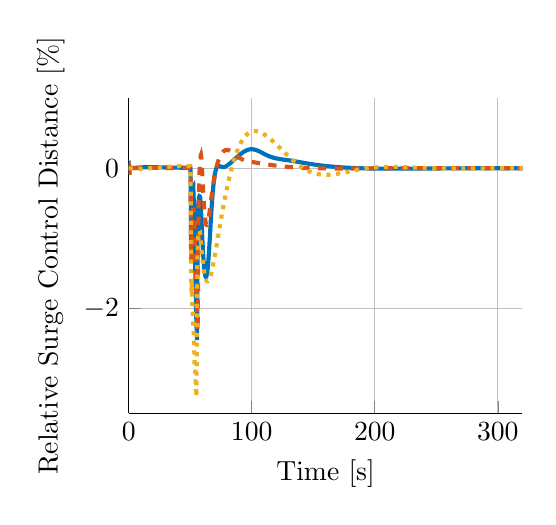
\begin{tikzpicture}

\begin{axis}[%
width=5cm,
height=4cm,
at={(0\linewidth,0\linewidth)},
scale only axis,
xmin=0,
xmax=320,
xlabel={Time [s]},
xmajorgrids,
ymin=-3.5,
ymax=1,
ylabel={Relative Surge Control Distance [\%]},
ymajorgrids,
axis background/.style={fill=white},
% title style={font=\bfseries},
% title={Surge Control Distance},
axis x line*=bottom,
axis y line*=left
]
\addplot [color=mycolor1,solid,line width=1.5pt,forget plot]
  table[row sep=crcr]{%
0	-0.0396000000000001\\
0.25	-0.0265199999999997\\
0.5	-0.0917099999999991\\
0.75	-0.0322300000000002\\
1	0.01417\\
1.25	0.00487000000000037\\
1.5	-0.0024299999999986\\
1.75	0.00156000000000134\\
2	0.00298000000000087\\
2.25	0.00211000000000006\\
2.5	0.00220999999999982\\
2.75	0.00270000000000081\\
3	0.00290999999999997\\
3.25	0.00311000000000128\\
3.5	0.00339000000000134\\
3.75	0.00366\\
4	0.00392000000000081\\
4.25	0.00416000000000061\\
4.5	0.0044000000000004\\
4.75	0.0046400000000002\\
5	0.00488\\
5.25	0.00513000000000119\\
5.5	0.00541000000000125\\
5.75	0.00572000000000017\\
6	0.00605999999999973\\
6.25	0.00641000000000069\\
6.5	0.0067800000000009\\
6.75	0.00716000000000072\\
7	0.00753000000000092\\
7.25	0.00788000000000011\\
7.5	0.00821999999999967\\
7.75	0.00853999999999999\\
8	0.00886000000000031\\
8.25	0.00917000000000101\\
8.5	0.00950000000000095\\
8.75	0.00983000000000089\\
9	0.0101800000000001\\
9.25	0.010530000000001\\
9.5	0.0108899999999998\\
9.75	0.0112400000000008\\
10	0.0115800000000004\\
10.25	0.0119000000000007\\
10.5	0.0122\\
10.75	0.0124700000000004\\
11	0.0127300000000012\\
11.25	0.012970000000001\\
11.5	0.0132100000000008\\
11.75	0.013440000000001\\
12	0.0136800000000008\\
12.25	0.0139200000000006\\
12.5	0.0141600000000004\\
12.75	0.0143900000000006\\
13	0.0146100000000011\\
13.25	0.0148100000000007\\
13.5	0.0149800000000013\\
13.75	0.0151200000000014\\
14	0.01525\\
14.25	0.0153499999999998\\
14.5	0.0154500000000013\\
14.75	0.0155500000000011\\
15	0.0156500000000008\\
15.25	0.0157500000000006\\
15.5	0.0158400000000007\\
15.75	0.0159300000000009\\
16	0.0160100000000014\\
16.25	0.0160800000000005\\
16.5	0.0161200000000008\\
16.75	0.01614\\
17	0.01614\\
17.25	0.0161300000000004\\
17.5	0.0161100000000012\\
17.75	0.0160800000000005\\
18	0.0160600000000013\\
18.25	0.0160499999999999\\
18.5	0.0160300000000007\\
18.75	0.016020000000001\\
19	0.0159900000000004\\
19.25	0.0159599999999998\\
19.5	0.0159099999999999\\
19.75	0.0158400000000007\\
20	0.0157600000000002\\
20.25	0.0156700000000001\\
20.5	0.0155700000000003\\
20.75	0.0154700000000005\\
21	0.0153700000000008\\
21.25	0.0152900000000002\\
21.5	0.0152000000000001\\
21.75	0.015130000000001\\
22	0.0150500000000005\\
22.25	0.0149600000000003\\
22.5	0.0148600000000005\\
22.75	0.0147500000000012\\
23	0.0146200000000007\\
23.25	0.0144900000000003\\
23.5	0.0143500000000003\\
23.75	0.0142199999999999\\
24	0.0140900000000013\\
24.25	0.0139700000000005\\
24.5	0.0138600000000011\\
24.75	0.0137600000000013\\
25	0.0136500000000002\\
25.25	0.0135500000000004\\
25.5	0.013440000000001\\
25.75	0.0133100000000006\\
26	0.0131800000000002\\
26.25	0.0130400000000002\\
26.5	0.0128900000000005\\
26.75	0.0127500000000005\\
27	0.0126200000000001\\
27.25	0.0124899999999997\\
27.5	0.0123800000000003\\
27.75	0.0122800000000005\\
28	0.0121800000000007\\
28.25	0.012080000000001\\
28.5	0.0119800000000012\\
28.75	0.0118600000000004\\
29	0.0117400000000014\\
29.25	0.011610000000001\\
29.5	0.011470000000001\\
29.75	0.0113400000000006\\
30	0.0112199999999998\\
30.25	0.0111100000000004\\
30.5	0.0110200000000003\\
30.75	0.0109300000000001\\
31	0.0108500000000014\\
31.25	0.0107700000000008\\
31.5	0.0106900000000003\\
31.75	0.0105900000000005\\
32	0.0104900000000008\\
32.25	0.0103800000000014\\
32.5	0.0102700000000002\\
32.75	0.0101600000000008\\
33	0.0100600000000011\\
33.25	0.00997000000000092\\
33.5	0.00990000000000002\\
33.75	0.00984000000000052\\
34	0.00978000000000101\\
34.25	0.00973000000000113\\
34.5	0.00966999999999985\\
34.75	0.00960000000000072\\
35	0.00952999999999982\\
35.25	0.00943999999999967\\
35.5	0.0093500000000013\\
35.75	0.00927000000000078\\
36	0.00919000000000025\\
36.25	0.00913000000000075\\
36.5	0.00908000000000087\\
36.75	0.0090400000000006\\
37	0.00900999999999996\\
37.25	0.00899000000000072\\
37.5	0.00895000000000046\\
37.75	0.0089100000000002\\
38	0.00886000000000031\\
38.25	0.00880000000000081\\
38.5	0.0087299999999999\\
38.75	0.0086700000000004\\
39	0.00861000000000089\\
39.25	0.00857000000000063\\
39.5	0.00855000000000139\\
39.75	0.00853000000000037\\
40	0.00853000000000037\\
40.25	0.00853000000000037\\
40.5	0.00852000000000075\\
40.75	0.00849999999999973\\
41	0.00847000000000087\\
41.25	0.00842000000000098\\
41.5	0.0083700000000011\\
41.75	0.00833000000000084\\
42	0.00829000000000057\\
42.25	0.00827000000000133\\
42.5	0.00825999999999993\\
42.75	0.00827000000000133\\
43	0.00829000000000057\\
43.25	0.00830999999999982\\
43.5	0.00832000000000122\\
43.75	0.00832000000000122\\
44	0.0083000000000002\\
44.25	0.00827000000000133\\
44.5	0.00823000000000107\\
44.75	0.00820000000000043\\
45	0.00818000000000119\\
45.25	0.00816999999999979\\
45.5	0.00818000000000119\\
45.75	0.00820000000000043\\
46	0.00824000000000069\\
46.25	0.00827000000000133\\
46.5	0.0083000000000002\\
46.75	0.00830999999999982\\
47	0.0083000000000002\\
47.25	0.00828000000000095\\
47.5	0.00825000000000031\\
47.75	0.00821999999999967\\
48	0.00821000000000005\\
48.25	0.00821000000000005\\
48.5	0.00823000000000107\\
48.75	0.00827000000000133\\
49	0.00832000000000122\\
49.25	0.0083599999999997\\
49.5	0.00839999999999996\\
49.75	0.00842000000000098\\
50	0.00842000000000098\\
50.25	-0.0222599999999993\\
50.5	-0.512049999999999\\
50.75	-1.18987\\
51	-1.03653\\
51.25	-0.638629999999999\\
51.5	-0.600519999999999\\
51.75	-0.56328\\
52	-0.395809999999999\\
52.25	-0.271539999999999\\
52.5	-0.264349999999999\\
52.75	-0.410279999999999\\
53	-0.48042\\
53.25	-0.60544\\
53.5	-0.88857\\
53.75	-1.15064\\
54	-1.35633\\
54.25	-1.57359\\
54.5	-1.7979\\
54.75	-2.00288\\
55	-2.18014\\
55.25	-2.34312\\
55.5	-2.45483\\
55.75	-1.84971\\
56	-1.09641\\
56.25	-0.735829999999999\\
56.5	-0.61009\\
56.75	-0.522939999999999\\
57	-0.452889999999999\\
57.25	-0.4091\\
57.5	-0.398529999999999\\
57.75	-0.40103\\
58	-0.412649999999999\\
58.25	-0.450679999999999\\
58.5	-0.51716\\
58.75	-0.599349999999999\\
59	-0.689609999999999\\
59.25	-0.785019999999999\\
59.5	-0.88153\\
59.75	-0.97535\\
60	-1.06446\\
60.25	-1.14778\\
60.5	-1.22434\\
60.75	-1.29329\\
61	-1.35421\\
61.25	-1.40701\\
61.5	-1.45168\\
61.75	-1.48822\\
62	-1.51667\\
62.25	-1.53712\\
62.5	-1.54962\\
62.75	-1.55422\\
63	-1.55096\\
63.25	-1.53989\\
63.5	-1.52107\\
63.75	-1.49462\\
64	-1.46069\\
64.25	-1.41953\\
64.5	-1.3715\\
64.75	-1.31706\\
65	-1.25681\\
65.25	-1.19147\\
65.5	-1.12185\\
65.75	-1.04889\\
66	-0.973579999999999\\
66.25	-0.897019999999999\\
66.5	-0.820359999999999\\
66.75	-0.7448\\
67	-0.671399999999999\\
67.25	-0.601019999999999\\
67.5	-0.534199999999999\\
67.75	-0.471299999999999\\
68	-0.4125\\
68.25	-0.357919999999999\\
68.5	-0.30758\\
68.75	-0.261449999999999\\
69	-0.21946\\
69.25	-0.18146\\
69.5	-0.1473\\
69.75	-0.116819999999999\\
70	-0.0898599999999998\\
70.25	-0.0662399999999987\\
70.5	-0.0457900000000002\\
70.75	-0.028319999999999\\
71	-0.0136000000000003\\
71.25	-0.00141999999999953\\
71.5	0.00846000000000124\\
71.75	0.0162700000000005\\
72	0.0222500000000014\\
72.25	0.0266200000000012\\
72.5	0.0296099999999999\\
72.75	0.0314200000000007\\
73	0.0322600000000008\\
73.25	0.0323100000000007\\
73.5	0.0317300000000014\\
73.75	0.0306700000000006\\
74	0.02928\\
74.25	0.0276700000000005\\
74.5	0.0259499999999999\\
74.75	0.0242100000000001\\
75	0.0225200000000001\\
75.25	0.0209500000000009\\
75.5	0.0195500000000006\\
75.75	0.0183600000000013\\
76	0.0174200000000013\\
76.25	0.0167400000000004\\
76.5	0.016350000000001\\
76.75	0.0162500000000012\\
77	0.0164500000000007\\
77.25	0.01694\\
77.5	0.0177200000000006\\
77.75	0.0187800000000014\\
78	0.0201100000000007\\
78.25	0.0216900000000013\\
78.5	0.0235099999999999\\
78.75	0.0255500000000008\\
79	0.0278000000000009\\
79.25	0.0302400000000009\\
79.5	0.0328600000000012\\
79.75	0.0356300000000012\\
80	0.0385500000000008\\
80.25	0.0416000000000007\\
80.5	0.0447600000000001\\
80.75	0.0480200000000011\\
81	0.05138\\
81.25	0.0548200000000012\\
81.5	0.0583200000000001\\
81.75	0.06189\\
82	0.0655099999999997\\
82.25	0.0691800000000011\\
82.5	0.072890000000001\\
82.75	0.0766400000000012\\
83	0.0804100000000005\\
83.25	0.0842200000000002\\
83.5	0.0880400000000012\\
83.75	0.0918900000000011\\
84	0.0957500000000007\\
84.25	0.0996300000000012\\
84.5	0.103520000000001\\
84.75	0.107420000000001\\
85	0.111330000000001\\
85.25	0.115250000000001\\
85.5	0.11917\\
85.75	0.123090000000001\\
86	0.12702\\
86.25	0.13095\\
86.5	0.134880000000001\\
86.75	0.138810000000001\\
87	0.14273\\
87.25	0.146650000000001\\
87.5	0.15056\\
87.75	0.15446\\
88	0.158340000000001\\
88.25	0.162220000000001\\
88.5	0.166070000000001\\
88.75	0.16991\\
89	0.173720000000001\\
89.25	0.17751\\
89.5	0.18126\\
89.75	0.184990000000001\\
90	0.188690000000001\\
90.25	0.19234\\
90.5	0.195960000000001\\
90.75	0.199530000000001\\
91	0.203050000000001\\
91.25	0.206520000000001\\
91.5	0.209940000000001\\
91.75	0.2133\\
92	0.2166\\
92.25	0.21983\\
92.5	0.222990000000001\\
92.75	0.226080000000001\\
93	0.229090000000001\\
93.25	0.23203\\
93.5	0.23488\\
93.75	0.237640000000001\\
94	0.240320000000001\\
94.25	0.242900000000001\\
94.5	0.24539\\
94.75	0.247780000000001\\
95	0.250070000000001\\
95.25	0.25226\\
95.5	0.254330000000001\\
95.75	0.256310000000001\\
96	0.25817\\
96.25	0.259910000000001\\
96.5	0.26155\\
96.75	0.263060000000001\\
97	0.26446\\
97.25	0.265740000000001\\
97.5	0.266910000000001\\
97.75	0.267950000000001\\
98	0.26887\\
98.25	0.269670000000001\\
98.5	0.270350000000001\\
98.75	0.270900000000001\\
99	0.27134\\
99.25	0.271650000000001\\
99.5	0.271850000000001\\
99.75	0.271930000000001\\
100	0.271890000000001\\
100.25	0.27173\\
100.5	0.271460000000001\\
100.75	0.271080000000001\\
101	0.270580000000001\\
101.25	0.26998\\
101.5	0.269270000000001\\
101.75	0.268460000000001\\
102	0.26755\\
102.25	0.266530000000001\\
102.5	0.26543\\
102.75	0.264230000000001\\
103	0.26294\\
103.25	0.261570000000001\\
103.5	0.260110000000001\\
103.75	0.25858\\
104	0.256970000000001\\
104.25	0.25529\\
104.5	0.253540000000001\\
104.75	0.25173\\
105	0.24986\\
105.25	0.24794\\
105.5	0.24596\\
105.75	0.243930000000001\\
106	0.241860000000001\\
106.25	0.23976\\
106.5	0.23761\\
106.75	0.235430000000001\\
107	0.233230000000001\\
107.25	0.231\\
107.5	0.22875\\
107.75	0.22648\\
108	0.2242\\
108.25	0.221910000000001\\
108.5	0.219610000000001\\
108.75	0.217310000000001\\
109	0.215010000000001\\
109.25	0.212710000000001\\
109.5	0.210420000000001\\
109.75	0.20814\\
110	0.205860000000001\\
110.25	0.203610000000001\\
110.5	0.201370000000001\\
110.75	0.199150000000001\\
111	0.196950000000001\\
111.25	0.19478\\
111.5	0.192630000000001\\
111.75	0.19051\\
112	0.188420000000001\\
112.25	0.186360000000001\\
112.5	0.184330000000001\\
112.75	0.18234\\
113	0.180380000000001\\
113.25	0.178460000000001\\
113.5	0.17657\\
113.75	0.174720000000001\\
114	0.17291\\
114.25	0.171140000000001\\
114.5	0.169410000000001\\
114.75	0.167720000000001\\
115	0.166070000000001\\
115.25	0.16446\\
115.5	0.162880000000001\\
115.75	0.161350000000001\\
116	0.15986\\
116.25	0.15841\\
116.5	0.157\\
116.75	0.155620000000001\\
117	0.15428\\
117.25	0.152980000000001\\
117.5	0.151720000000001\\
117.75	0.150500000000001\\
118	0.1493\\
118.25	0.148150000000001\\
118.5	0.147020000000001\\
118.75	0.14593\\
119	0.144880000000001\\
119.25	0.14385\\
119.5	0.142850000000001\\
119.75	0.14188\\
120	0.140930000000001\\
120.25	0.14002\\
120.5	0.13912\\
120.75	0.138260000000001\\
121	0.137410000000001\\
121.25	0.13659\\
121.5	0.13578\\
121.75	0.135\\
122	0.134230000000001\\
122.25	0.13348\\
122.5	0.13275\\
122.75	0.13203\\
123	0.13133\\
123.25	0.130640000000001\\
123.5	0.129950000000001\\
123.75	0.129290000000001\\
124	0.128630000000001\\
124.25	0.127970000000001\\
124.5	0.127330000000001\\
124.75	0.12669\\
125	0.126060000000001\\
125.25	0.125440000000001\\
125.5	0.12481\\
125.75	0.1242\\
126	0.12358\\
126.25	0.12297\\
126.5	0.12236\\
126.75	0.121740000000001\\
127	0.121130000000001\\
127.25	0.120520000000001\\
127.5	0.119910000000001\\
127.75	0.119290000000001\\
128	0.118680000000001\\
128.25	0.11806\\
128.5	0.117430000000001\\
128.75	0.116810000000001\\
129	0.11618\\
129.25	0.115550000000001\\
129.5	0.11491\\
129.75	0.114270000000001\\
130	0.113620000000001\\
130.25	0.112970000000001\\
130.5	0.11232\\
130.75	0.111660000000001\\
131	0.110990000000001\\
131.25	0.11032\\
131.5	0.109640000000001\\
131.75	0.10896\\
132	0.108270000000001\\
132.25	0.10758\\
132.5	0.10688\\
132.75	0.10618\\
133	0.10547\\
133.25	0.104760000000001\\
133.5	0.104040000000001\\
133.75	0.10332\\
134	0.102590000000001\\
134.25	0.10186\\
134.5	0.10112\\
134.75	0.100380000000001\\
135	0.0996400000000008\\
135.25	0.0988900000000008\\
135.5	0.0981400000000008\\
135.75	0.0973800000000011\\
136	0.0966199999999997\\
136.25	0.0958600000000001\\
136.5	0.0950900000000008\\
136.75	0.0943300000000011\\
137	0.0935600000000001\\
137.25	0.0927900000000008\\
137.5	0.0920100000000001\\
137.75	0.0912400000000009\\
138	0.0904600000000002\\
138.25	0.0896800000000013\\
138.5	0.0889000000000006\\
138.75	0.08812\\
139	0.0873400000000011\\
139.25	0.0865600000000004\\
139.5	0.0857799999999997\\
139.75	0.0850000000000009\\
140	0.0842200000000002\\
140.25	0.0834400000000013\\
140.5	0.0826600000000006\\
140.75	0.0818900000000014\\
141	0.0811100000000007\\
141.25	0.0803400000000014\\
141.5	0.0795600000000007\\
141.75	0.0787899999999997\\
142	0.0780200000000004\\
142.25	0.0772600000000008\\
142.5	0.0764899999999997\\
142.75	0.0757300000000001\\
143	0.0749700000000004\\
143.25	0.0742100000000008\\
143.5	0.0734600000000007\\
143.75	0.0727100000000007\\
144	0.0719600000000007\\
144.25	0.0712200000000003\\
144.5	0.0704799999999999\\
144.75	0.0697400000000012\\
145	0.0690100000000005\\
145.25	0.0682799999999997\\
145.5	0.0675500000000007\\
145.75	0.0668300000000013\\
146	0.0661100000000001\\
146.25	0.0654000000000003\\
146.5	0.0646900000000006\\
146.75	0.0639900000000004\\
147	0.0632900000000003\\
147.25	0.0625900000000001\\
147.5	0.0619000000000014\\
147.75	0.0612100000000009\\
148	0.06053\\
148.25	0.0598500000000008\\
148.5	0.0591800000000013\\
148.75	0.0585100000000001\\
149	0.0578400000000006\\
149.25	0.0571800000000007\\
149.5	0.0565300000000004\\
149.75	0.0558800000000002\\
150	0.0552299999999999\\
150.25	0.054590000000001\\
150.5	0.0539500000000004\\
150.75	0.0533200000000011\\
151	0.0526900000000001\\
151.25	0.0520700000000005\\
151.5	0.0514500000000009\\
151.75	0.0508400000000009\\
152	0.0502300000000009\\
152.25	0.0496200000000009\\
152.5	0.0490200000000005\\
152.75	0.0484299999999998\\
153	0.0478400000000008\\
153.25	0.04725\\
153.5	0.0466700000000007\\
153.75	0.0460900000000013\\
154	0.0455199999999998\\
154.25	0.04495\\
154.5	0.0443800000000003\\
154.75	0.0438200000000002\\
155	0.0432699999999997\\
155.25	0.042720000000001\\
155.5	0.0421700000000005\\
155.75	0.04162\\
156	0.0410900000000005\\
156.25	0.0405500000000014\\
156.5	0.0400200000000002\\
156.75	0.0394900000000007\\
157	0.0389700000000008\\
157.25	0.038450000000001\\
157.5	0.0379400000000008\\
157.75	0.0374300000000005\\
158	0.0369200000000003\\
158.25	0.0364199999999997\\
158.5	0.0359200000000008\\
158.75	0.0354200000000002\\
159	0.034930000000001\\
159.25	0.03444\\
159.5	0.0339600000000004\\
159.75	0.0334800000000008\\
160	0.0330000000000013\\
160.25	0.0325300000000013\\
160.5	0.0320600000000013\\
160.75	0.031600000000001\\
161	0.0311400000000006\\
161.25	0.0306800000000003\\
161.5	0.0302199999999999\\
161.75	0.029770000000001\\
162	0.0293299999999999\\
162.25	0.0288800000000009\\
162.5	0.0284399999999998\\
162.75	0.0280100000000001\\
163	0.0275700000000008\\
163.25	0.0271400000000011\\
163.5	0.026720000000001\\
163.75	0.0263000000000009\\
164	0.0258800000000008\\
164.25	0.0254600000000007\\
164.5	0.0250500000000002\\
164.75	0.0246399999999998\\
165	0.0242300000000011\\
165.25	0.0238300000000002\\
165.5	0.0234300000000012\\
165.75	0.0230399999999999\\
166	0.0226500000000005\\
166.25	0.0222600000000011\\
166.5	0.0218699999999998\\
166.75	0.02149\\
167	0.0211100000000002\\
167.25	0.02074\\
167.5	0.0203699999999998\\
167.75	0.0200000000000014\\
168	0.0196300000000011\\
168.25	0.0192700000000006\\
168.5	0.01891\\
168.75	0.0185600000000008\\
169	0.0182000000000002\\
169.25	0.0178600000000007\\
169.5	0.0175099999999997\\
169.75	0.0171700000000001\\
170	0.0168300000000006\\
170.25	0.016490000000001\\
170.5	0.0161600000000011\\
170.75	0.0158300000000011\\
171	0.0155000000000012\\
171.25	0.0151800000000009\\
171.5	0.0148600000000005\\
171.75	0.0145400000000002\\
172	0.0142300000000013\\
172.25	0.0139200000000006\\
172.5	0.0136099999999999\\
172.75	0.0133100000000006\\
173	0.0130100000000013\\
173.25	0.0127100000000002\\
173.5	0.0124100000000009\\
173.75	0.0121200000000012\\
174	0.0118299999999998\\
174.25	0.0115499999999997\\
174.5	0.0112699999999997\\
174.75	0.0109900000000014\\
175	0.0107100000000013\\
175.25	0.0104400000000009\\
175.5	0.0101700000000005\\
175.75	0.00990000000000002\\
176	0.00963000000000136\\
176.25	0.00937000000000054\\
176.5	0.00910999999999973\\
176.75	0.00886000000000031\\
177	0.00861000000000089\\
177.25	0.0083599999999997\\
177.5	0.00811000000000028\\
177.75	0.00787000000000049\\
178	0.00762000000000107\\
178.25	0.0073900000000009\\
178.5	0.0071500000000011\\
178.75	0.00692000000000093\\
179	0.00669000000000075\\
179.25	0.00646000000000058\\
179.5	0.00624000000000002\\
179.75	0.00602000000000125\\
180	0.00580000000000069\\
180.25	0.00558000000000014\\
180.5	0.00537000000000099\\
180.75	0.00516000000000005\\
181	0.0049500000000009\\
181.25	0.00475000000000136\\
181.5	0.00455000000000005\\
181.75	0.00435000000000052\\
182	0.00415000000000099\\
182.25	0.00396000000000107\\
182.5	0.00375999999999976\\
182.75	0.00358000000000125\\
183	0.00339000000000134\\
183.25	0.00320000000000142\\
183.5	0.00302000000000113\\
183.75	0.00284000000000084\\
184	0.00267000000000017\\
184.25	0.00248999999999988\\
184.5	0.00232000000000099\\
184.75	0.00215000000000032\\
185	0.00199000000000105\\
185.25	0.00182000000000038\\
185.5	0.00166000000000111\\
185.75	0.00150000000000006\\
186	0.00134000000000079\\
186.25	0.00119000000000113\\
186.5	0.00103999999999971\\
186.75	0.000890000000000057\\
187	0.000740000000000407\\
187.25	0.000590000000000757\\
187.5	0.000450000000000728\\
187.75	0.000310000000000699\\
188	0.00017000000000067\\
188.25	3.00000000006406e-05\\
188.5	-9.99999999997669e-05\\
188.75	-0.000230000000000175\\
189	-0.000370000000000203\\
189.25	-0.000489999999999213\\
189.5	-0.000619999999999621\\
189.75	-0.000739999999998631\\
190	-0.000869999999999038\\
190.25	-0.000989999999999824\\
190.5	-0.00109999999999921\\
190.75	-0.00122\\
191	-0.00132999999999939\\
191.25	-0.00145000000000017\\
191.5	-0.00155999999999956\\
191.75	-0.00165999999999933\\
192	-0.00176999999999872\\
192.25	-0.00187999999999988\\
192.5	-0.00197999999999965\\
192.75	-0.00207999999999942\\
193	-0.00217999999999918\\
193.25	-0.00227999999999895\\
193.5	-0.0023699999999991\\
193.75	-0.00245999999999924\\
194	-0.00255999999999901\\
194.25	-0.00264999999999915\\
194.5	-0.00272999999999968\\
194.75	-0.00281999999999982\\
195	-0.00290999999999997\\
195.25	-0.00298999999999872\\
195.5	-0.00306999999999924\\
195.75	-0.00314999999999976\\
196	-0.00323000000000029\\
196.25	-0.00329999999999941\\
196.5	-0.00337999999999994\\
196.75	-0.00344999999999906\\
197	-0.00351999999999997\\
197.25	-0.00359999999999872\\
197.5	-0.00366\\
197.75	-0.00372999999999912\\
198	-0.00380000000000003\\
198.25	-0.00385999999999953\\
198.5	-0.00391999999999904\\
198.75	-0.00398999999999994\\
199	-0.00404999999999944\\
199.25	-0.00409999999999933\\
199.5	-0.00415999999999883\\
199.75	-0.00422000000000011\\
200	-0.00427\\
200.25	-0.00431999999999988\\
200.5	-0.00437999999999938\\
200.75	-0.00442999999999927\\
201	-0.00447999999999915\\
201.25	-0.00451999999999941\\
201.5	-0.0045699999999993\\
201.75	-0.00460999999999956\\
202	-0.00465999999999944\\
202.25	-0.0046999999999997\\
202.5	-0.00473999999999997\\
202.75	-0.00478000000000023\\
203	-0.00481999999999871\\
203.25	-0.00485999999999898\\
203.5	-0.00489999999999924\\
203.75	-0.00492999999999988\\
204	-0.00497000000000014\\
204.25	-0.00499999999999901\\
204.5	-0.00502999999999965\\
204.75	-0.00506000000000029\\
205	-0.00508999999999915\\
205.25	-0.00511999999999979\\
205.5	-0.00514999999999866\\
205.75	-0.0051799999999993\\
206	-0.00520000000000032\\
206.25	-0.00522999999999918\\
206.5	-0.0052500000000002\\
206.75	-0.00526999999999944\\
207	-0.00530000000000008\\
207.25	-0.00531999999999933\\
207.5	-0.00533999999999857\\
207.75	-0.00535999999999959\\
208	-0.00536999999999921\\
208.25	-0.00539000000000023\\
208.5	-0.00540999999999947\\
208.75	-0.00541999999999909\\
209	-0.00544000000000011\\
209.25	-0.00544999999999973\\
209.5	-0.00545999999999935\\
209.75	-0.0054799999999986\\
210	-0.00548999999999999\\
210.25	-0.00549999999999962\\
210.5	-0.00550999999999924\\
210.75	-0.00551999999999886\\
211	-0.00551999999999886\\
211.25	-0.00553000000000026\\
211.5	-0.00553999999999988\\
211.75	-0.00553999999999988\\
212	-0.0055499999999995\\
212.25	-0.0055499999999995\\
212.5	-0.00555999999999912\\
212.75	-0.00555999999999912\\
213	-0.00555999999999912\\
213.25	-0.00555999999999912\\
213.5	-0.00555999999999912\\
213.75	-0.00555999999999912\\
214	-0.00555999999999912\\
214.25	-0.00555999999999912\\
214.5	-0.00555999999999912\\
214.75	-0.00555999999999912\\
215	-0.0055499999999995\\
215.25	-0.0055499999999995\\
215.5	-0.0055499999999995\\
215.75	-0.00553999999999988\\
216	-0.00553999999999988\\
216.25	-0.00553000000000026\\
216.5	-0.00551999999999886\\
216.75	-0.00551999999999886\\
217	-0.00550999999999924\\
217.25	-0.00549999999999962\\
217.5	-0.00548999999999999\\
217.75	-0.0054799999999986\\
218	-0.00546999999999898\\
218.25	-0.00545999999999935\\
218.5	-0.00544999999999973\\
218.75	-0.00544000000000011\\
219	-0.00542999999999871\\
219.25	-0.00541999999999909\\
219.5	-0.00540999999999947\\
219.75	-0.00539000000000023\\
220	-0.00537999999999883\\
220.25	-0.00536999999999921\\
220.5	-0.00534999999999997\\
220.75	-0.00533999999999857\\
221	-0.00531999999999933\\
221.25	-0.0053099999999997\\
221.5	-0.00528999999999868\\
221.75	-0.00527999999999906\\
222	-0.00525999999999982\\
222.25	-0.0052500000000002\\
222.5	-0.00522999999999918\\
222.75	-0.00520999999999994\\
223	-0.00518999999999892\\
223.25	-0.0051799999999993\\
223.5	-0.00516000000000005\\
223.75	-0.00513999999999903\\
224	-0.00511999999999979\\
224.25	-0.00509999999999877\\
224.5	-0.00507999999999953\\
224.75	-0.00506000000000029\\
225	-0.00503999999999927\\
225.25	-0.00502000000000002\\
225.5	-0.00499999999999901\\
225.75	-0.00497999999999976\\
226	-0.00495999999999874\\
226.25	-0.0049399999999995\\
226.5	-0.00492000000000026\\
226.75	-0.00489999999999924\\
227	-0.00488\\
227.25	-0.00484999999999935\\
227.5	-0.00483000000000011\\
227.75	-0.00480999999999909\\
228	-0.00478999999999985\\
228.25	-0.00475999999999921\\
228.5	-0.00473999999999997\\
228.75	-0.00471999999999895\\
229	-0.00469000000000008\\
229.25	-0.00466999999999906\\
229.5	-0.00464999999999982\\
229.75	-0.00461999999999918\\
230	-0.00459999999999994\\
230.25	-0.0045699999999993\\
230.5	-0.00455000000000005\\
230.75	-0.00452999999999903\\
231	-0.00450000000000017\\
231.25	-0.00447999999999915\\
231.5	-0.00445000000000029\\
231.75	-0.00442999999999927\\
232	-0.00439999999999863\\
232.25	-0.00437999999999938\\
232.5	-0.00434999999999874\\
232.75	-0.0043299999999995\\
233	-0.00429999999999886\\
233.25	-0.00427999999999962\\
233.5	-0.00424999999999898\\
233.75	-0.00422999999999973\\
234	-0.00419999999999909\\
234.25	-0.00417000000000023\\
234.5	-0.00414999999999921\\
234.75	-0.00411999999999857\\
235	-0.00409999999999933\\
235.25	-0.00406999999999869\\
235.5	-0.00403999999999982\\
235.75	-0.0040199999999988\\
236	-0.00398999999999994\\
236.25	-0.00396999999999892\\
236.5	-0.00394000000000005\\
236.75	-0.00390999999999941\\
237	-0.00389000000000017\\
237.25	-0.00385999999999953\\
237.5	-0.00382999999999889\\
237.75	-0.00380999999999965\\
238	-0.00377999999999901\\
238.25	-0.00375999999999976\\
238.5	-0.00372999999999912\\
238.75	-0.00370000000000026\\
239	-0.00367999999999924\\
239.25	-0.0036499999999986\\
239.5	-0.00361999999999973\\
239.75	-0.00359999999999872\\
240	-0.00356999999999985\\
240.25	-0.00354999999999883\\
240.5	-0.00351999999999997\\
240.75	-0.00348999999999933\\
241	-0.00347000000000008\\
241.25	-0.00343999999999944\\
241.5	-0.0034099999999988\\
241.75	-0.00338999999999956\\
242	-0.00335999999999892\\
242.25	-0.00333999999999968\\
242.5	-0.00330999999999904\\
242.75	-0.00328000000000017\\
243	-0.00325999999999915\\
243.25	-0.00323000000000029\\
243.5	-0.00320999999999927\\
243.75	-0.00317999999999863\\
244	-0.00315999999999939\\
244.25	-0.00312999999999874\\
244.5	-0.00309999999999988\\
244.75	-0.00307999999999886\\
245	-0.00305\\
245.25	-0.00302999999999898\\
245.5	-0.00300000000000011\\
245.75	-0.00297999999999909\\
246	-0.00295000000000023\\
246.25	-0.00292999999999921\\
246.5	-0.00289999999999857\\
246.75	-0.00287999999999933\\
247	-0.00284999999999869\\
247.25	-0.00282999999999944\\
247.5	-0.0027999999999988\\
247.75	-0.00277999999999956\\
248	-0.00274999999999892\\
248.25	-0.00272999999999968\\
248.5	-0.00269999999999904\\
248.75	-0.00267999999999979\\
249	-0.00264999999999915\\
249.25	-0.00262999999999991\\
249.5	-0.00260999999999889\\
249.75	-0.00258000000000003\\
250	-0.00255999999999901\\
250.25	-0.00253000000000014\\
250.5	-0.00250999999999912\\
250.75	-0.00248999999999988\\
251	-0.00245999999999924\\
251.25	-0.00244\\
251.5	-0.00241999999999898\\
251.75	-0.00239000000000011\\
252	-0.0023699999999991\\
252.25	-0.00234999999999985\\
252.5	-0.00231999999999921\\
252.75	-0.00229999999999997\\
253	-0.00227999999999895\\
253.25	-0.00225999999999971\\
253.5	-0.00222999999999907\\
253.75	-0.00220999999999982\\
254	-0.0021899999999988\\
254.25	-0.00216999999999956\\
254.5	-0.00213999999999892\\
254.75	-0.00211999999999968\\
255	-0.00209999999999866\\
255.25	-0.00207999999999942\\
255.5	-0.00206000000000017\\
255.75	-0.00203999999999915\\
256	-0.00201000000000029\\
256.25	-0.00198999999999927\\
256.5	-0.00197000000000003\\
256.75	-0.00194999999999901\\
257	-0.00192999999999977\\
257.25	-0.00190999999999875\\
257.5	-0.0018899999999995\\
257.75	-0.00187000000000026\\
258	-0.00184999999999924\\
258.25	-0.00183\\
258.5	-0.00180999999999898\\
258.75	-0.00178999999999974\\
259	-0.00176999999999872\\
259.25	-0.00174999999999947\\
259.5	-0.00173000000000023\\
259.75	-0.00170999999999921\\
260	-0.00168999999999997\\
260.25	-0.00166999999999895\\
260.5	-0.00164999999999971\\
260.75	-0.00162999999999869\\
261	-0.00160999999999945\\
261.25	-0.0015900000000002\\
261.5	-0.0015799999999988\\
261.75	-0.00155999999999956\\
262	-0.00154000000000032\\
262.25	-0.0015199999999993\\
262.5	-0.00150000000000006\\
262.75	-0.00147999999999904\\
263	-0.00146999999999942\\
263.25	-0.00145000000000017\\
263.5	-0.00142999999999915\\
263.75	-0.00140999999999991\\
264	-0.00138999999999889\\
264.25	-0.00137999999999927\\
264.5	-0.00136000000000003\\
264.75	-0.00133999999999901\\
265	-0.00132999999999939\\
265.25	-0.00131000000000014\\
265.5	-0.00128999999999913\\
265.75	-0.0012799999999995\\
266	-0.00126000000000026\\
266.25	-0.00123999999999924\\
266.5	-0.00122999999999962\\
266.75	-0.0012099999999986\\
267	-0.00118999999999936\\
267.25	-0.00117999999999974\\
267.5	-0.00115999999999872\\
267.75	-0.0011499999999991\\
268	-0.00112999999999985\\
268.25	-0.00112000000000023\\
268.5	-0.00109999999999921\\
268.75	-0.00108999999999959\\
269	-0.00106999999999857\\
269.25	-0.00105999999999895\\
269.5	-0.00103999999999971\\
269.75	-0.00103000000000009\\
270	-0.00100999999999907\\
270.25	-0.000999999999999446\\
270.5	-0.000980000000000203\\
270.75	-0.000969999999998805\\
271	-0.000959999999999184\\
271.25	-0.000939999999999941\\
271.5	-0.000930000000000319\\
271.75	-0.0009099999999993\\
272	-0.000899999999999679\\
272.25	-0.000890000000000057\\
272.5	-0.000869999999999038\\
272.75	-0.000859999999999417\\
273	-0.000849999999999795\\
273.25	-0.000829999999998776\\
273.5	-0.000819999999999155\\
273.75	-0.000809999999999533\\
274	-0.000799999999999912\\
274.25	-0.000779999999998893\\
274.5	-0.000769999999999271\\
274.75	-0.00075999999999965\\
275	-0.000750000000000028\\
275.25	-0.000739999999998631\\
275.5	-0.000719999999999388\\
275.75	-0.000709999999999766\\
276	-0.000700000000000145\\
276.25	-0.000689999999998747\\
276.5	-0.000679999999999126\\
276.75	-0.000669999999999504\\
277	-0.000650000000000261\\
277.25	-0.000639999999998864\\
277.5	-0.000629999999999242\\
277.75	-0.000619999999999621\\
278	-0.000609999999999999\\
278.25	-0.000599999999998602\\
278.5	-0.00058999999999898\\
278.75	-0.000579999999999359\\
279	-0.000569999999999737\\
279.25	-0.000560000000000116\\
279.5	-0.000549999999998718\\
279.75	-0.000539999999999097\\
280	-0.000529999999999475\\
280.25	-0.000519999999999854\\
280.5	-0.000510000000000232\\
280.75	-0.000499999999998835\\
281	-0.000489999999999213\\
281.25	-0.000479999999999592\\
281.5	-0.00046999999999997\\
281.75	-0.000459999999998573\\
282	-0.000449999999998951\\
282.25	-0.00043999999999933\\
282.5	-0.000429999999999708\\
282.75	-0.000420000000000087\\
283	-0.000409999999998689\\
283.25	-0.000409999999998689\\
283.5	-0.000399999999999068\\
283.75	-0.000389999999999446\\
284	-0.000379999999999825\\
284.25	-0.000370000000000203\\
284.5	-0.000359999999998806\\
284.75	-0.000359999999998806\\
285	-0.000349999999999184\\
285.25	-0.000339999999999563\\
285.5	-0.000329999999999941\\
285.75	-0.00032000000000032\\
286	-0.00032000000000032\\
286.25	-0.000309999999998922\\
286.5	-0.000299999999999301\\
286.75	-0.000289999999999679\\
287	-0.000289999999999679\\
287.25	-0.000280000000000058\\
287.5	-0.00026999999999866\\
287.75	-0.00026999999999866\\
288	-0.000259999999999039\\
288.25	-0.000249999999999417\\
288.5	-0.000239999999999796\\
288.75	-0.000239999999999796\\
289	-0.000230000000000175\\
289.25	-0.000219999999998777\\
289.5	-0.000219999999998777\\
289.75	-0.000209999999999155\\
290	-0.000209999999999155\\
290.25	-0.000199999999999534\\
290.5	-0.000189999999999912\\
290.75	-0.000189999999999912\\
291	-0.000180000000000291\\
291.25	-0.000169999999998893\\
291.5	-0.000169999999998893\\
291.75	-0.000159999999999272\\
292	-0.000159999999999272\\
292.25	-0.00014999999999965\\
292.5	-0.00014999999999965\\
292.75	-0.000140000000000029\\
293	-0.000140000000000029\\
293.25	-0.000129999999998631\\
293.5	-0.00011999999999901\\
293.75	-0.00011999999999901\\
294	-0.000109999999999388\\
294.25	-0.000109999999999388\\
294.5	-9.99999999997669e-05\\
294.75	-9.99999999997669e-05\\
295	-9.00000000001455e-05\\
295.25	-9.00000000001455e-05\\
295.5	-9.00000000001455e-05\\
295.75	-7.99999999987477e-05\\
296	-7.99999999987477e-05\\
296.25	-6.99999999991263e-05\\
296.5	-6.99999999991263e-05\\
296.75	-5.99999999995049e-05\\
297	-5.99999999995049e-05\\
297.25	-4.99999999998835e-05\\
297.5	-4.99999999998835e-05\\
297.75	-4.99999999998835e-05\\
298	-4.0000000000262e-05\\
298.25	-4.0000000000262e-05\\
298.5	-2.99999999988643e-05\\
298.75	-2.99999999988643e-05\\
299	-2.99999999988643e-05\\
299.25	-1.99999999992428e-05\\
299.5	-1.99999999992428e-05\\
299.75	-1.99999999992428e-05\\
300	-9.99999999962142e-06\\
300.25	-9.99999999962142e-06\\
300.5	0\\
300.75	0\\
301	0\\
301.25	1.00000000013978e-05\\
301.5	1.00000000013978e-05\\
301.75	1.00000000013978e-05\\
302	2.00000000010192e-05\\
302.25	2.00000000010192e-05\\
302.5	2.00000000010192e-05\\
302.75	2.00000000010192e-05\\
303	3.00000000006406e-05\\
303.25	3.00000000006406e-05\\
303.5	3.00000000006406e-05\\
303.75	4.0000000000262e-05\\
304	4.0000000000262e-05\\
304.25	4.0000000000262e-05\\
304.5	4.0000000000262e-05\\
304.75	4.99999999998835e-05\\
305	4.99999999998835e-05\\
305.25	4.99999999998835e-05\\
305.5	4.99999999998835e-05\\
305.75	6.00000000012813e-05\\
306	6.00000000012813e-05\\
306.25	6.00000000012813e-05\\
306.5	6.00000000012813e-05\\
306.75	7.00000000009027e-05\\
307	7.00000000009027e-05\\
307.25	7.00000000009027e-05\\
307.5	7.00000000009027e-05\\
307.75	7.00000000009027e-05\\
308	8.00000000005241e-05\\
308.25	8.00000000005241e-05\\
308.5	8.00000000005241e-05\\
308.75	8.00000000005241e-05\\
309	8.00000000005241e-05\\
309.25	8.00000000005241e-05\\
309.5	9.00000000001455e-05\\
309.75	9.00000000001455e-05\\
310	9.00000000001455e-05\\
310.25	9.00000000001455e-05\\
310.5	9.00000000001455e-05\\
310.75	9.00000000001455e-05\\
311	9.99999999997669e-05\\
311.25	9.99999999997669e-05\\
311.5	9.99999999997669e-05\\
311.75	9.99999999997669e-05\\
312	9.99999999997669e-05\\
312.25	9.99999999997669e-05\\
312.5	9.99999999997669e-05\\
312.75	0.000110000000001165\\
313	0.000110000000001165\\
313.25	0.000110000000001165\\
313.5	0.000110000000001165\\
313.75	0.000110000000001165\\
314	0.000110000000001165\\
314.25	0.000110000000001165\\
314.5	0.000110000000001165\\
314.75	0.000110000000001165\\
315	0.000120000000000786\\
315.25	0.000120000000000786\\
315.5	0.000120000000000786\\
315.75	0.000120000000000786\\
316	0.000120000000000786\\
316.25	0.000120000000000786\\
316.5	0.000120000000000786\\
316.75	0.000120000000000786\\
317	0.000120000000000786\\
317.25	0.000120000000000786\\
317.5	0.000120000000000786\\
317.75	0.000130000000000408\\
318	0.000130000000000408\\
318.25	0.000130000000000408\\
318.5	0.000130000000000408\\
318.75	0.000130000000000408\\
319	0.000130000000000408\\
319.25	0.000130000000000408\\
319.5	0.000130000000000408\\
319.75	0.000130000000000408\\
320	0.000130000000000408\\
320.25	0.000130000000000408\\
320.5	0.000130000000000408\\
320.75	0.000130000000000408\\
321	0.000130000000000408\\
321.25	0.000130000000000408\\
321.5	0.000130000000000408\\
321.75	0.000130000000000408\\
322	0.000130000000000408\\
322.25	0.000130000000000408\\
322.5	0.000130000000000408\\
322.75	0.000130000000000408\\
323	0.000130000000000408\\
323.25	0.000130000000000408\\
323.5	0.000130000000000408\\
323.75	0.000130000000000408\\
324	0.000130000000000408\\
324.25	0.000130000000000408\\
324.5	0.000130000000000408\\
324.75	0.000130000000000408\\
325	0.000140000000000029\\
325.25	0.000140000000000029\\
325.5	0.000140000000000029\\
325.75	0.000140000000000029\\
326	0.000140000000000029\\
326.25	0.000140000000000029\\
326.5	0.000140000000000029\\
326.75	0.000140000000000029\\
327	0.000140000000000029\\
327.25	0.000130000000000408\\
327.5	0.000130000000000408\\
327.75	0.000130000000000408\\
328	0.000130000000000408\\
328.25	0.000130000000000408\\
328.5	0.000130000000000408\\
328.75	0.000130000000000408\\
329	0.000130000000000408\\
329.25	0.000130000000000408\\
329.5	0.000130000000000408\\
329.75	0.000130000000000408\\
330	0.000130000000000408\\
330.25	0.000130000000000408\\
330.5	0.000130000000000408\\
330.75	0.000130000000000408\\
331	0.000130000000000408\\
331.25	0.000130000000000408\\
331.5	0.000130000000000408\\
331.75	0.000130000000000408\\
332	0.000130000000000408\\
332.25	0.000130000000000408\\
332.5	0.000130000000000408\\
332.75	0.000130000000000408\\
333	0.000130000000000408\\
333.25	0.000130000000000408\\
333.5	0.000130000000000408\\
333.75	0.000130000000000408\\
334	0.000130000000000408\\
334.25	0.000130000000000408\\
334.5	0.000130000000000408\\
334.75	0.000130000000000408\\
335	0.000130000000000408\\
335.25	0.000130000000000408\\
335.5	0.000130000000000408\\
335.75	0.000130000000000408\\
336	0.000120000000000786\\
336.25	0.000120000000000786\\
336.5	0.000120000000000786\\
336.75	0.000120000000000786\\
337	0.000120000000000786\\
337.25	0.000120000000000786\\
337.5	0.000120000000000786\\
337.75	0.000120000000000786\\
338	0.000120000000000786\\
338.25	0.000120000000000786\\
338.5	0.000120000000000786\\
338.75	0.000120000000000786\\
339	0.000120000000000786\\
339.25	0.000120000000000786\\
339.5	0.000120000000000786\\
339.75	0.000120000000000786\\
340	0.000120000000000786\\
340.25	0.000120000000000786\\
340.5	0.000120000000000786\\
340.75	0.000120000000000786\\
341	0.000110000000001165\\
341.25	0.000110000000001165\\
341.5	0.000110000000001165\\
341.75	0.000110000000001165\\
342	0.000110000000001165\\
342.25	0.000110000000001165\\
342.5	0.000110000000001165\\
342.75	0.000110000000001165\\
343	0.000110000000001165\\
343.25	0.000110000000001165\\
343.5	0.000110000000001165\\
343.75	0.000110000000001165\\
344	0.000110000000001165\\
344.25	0.000110000000001165\\
344.5	0.000110000000001165\\
344.75	0.000110000000001165\\
345	0.000110000000001165\\
345.25	9.99999999997669e-05\\
345.5	9.99999999997669e-05\\
345.75	9.99999999997669e-05\\
346	9.99999999997669e-05\\
346.25	9.99999999997669e-05\\
346.5	9.99999999997669e-05\\
346.75	9.99999999997669e-05\\
347	9.99999999997669e-05\\
347.25	9.99999999997669e-05\\
347.5	9.99999999997669e-05\\
347.75	9.99999999997669e-05\\
348	9.99999999997669e-05\\
348.25	9.99999999997669e-05\\
348.5	9.99999999997669e-05\\
348.75	9.99999999997669e-05\\
349	9.99999999997669e-05\\
349.25	9.00000000001455e-05\\
349.5	9.00000000001455e-05\\
349.75	9.00000000001455e-05\\
350	9.00000000001455e-05\\
350.25	9.00000000001455e-05\\
350.5	9.00000000001455e-05\\
350.75	9.00000000001455e-05\\
351	9.00000000001455e-05\\
351.25	9.00000000001455e-05\\
351.5	9.00000000001455e-05\\
351.75	9.00000000001455e-05\\
352	9.00000000001455e-05\\
352.25	9.00000000001455e-05\\
352.5	9.00000000001455e-05\\
352.75	9.00000000001455e-05\\
353	8.00000000005241e-05\\
353.25	8.00000000005241e-05\\
353.5	8.00000000005241e-05\\
353.75	8.00000000005241e-05\\
354	8.00000000005241e-05\\
354.25	8.00000000005241e-05\\
354.5	8.00000000005241e-05\\
354.75	8.00000000005241e-05\\
355	8.00000000005241e-05\\
355.25	8.00000000005241e-05\\
355.5	8.00000000005241e-05\\
355.75	8.00000000005241e-05\\
356	8.00000000005241e-05\\
356.25	8.00000000005241e-05\\
356.5	8.00000000005241e-05\\
356.75	8.00000000005241e-05\\
357	7.00000000009027e-05\\
357.25	7.00000000009027e-05\\
357.5	7.00000000009027e-05\\
357.75	7.00000000009027e-05\\
358	7.00000000009027e-05\\
358.25	7.00000000009027e-05\\
358.5	7.00000000009027e-05\\
358.75	7.00000000009027e-05\\
359	7.00000000009027e-05\\
359.25	7.00000000009027e-05\\
359.5	7.00000000009027e-05\\
359.75	7.00000000009027e-05\\
360	7.00000000009027e-05\\
360.25	7.00000000009027e-05\\
360.5	7.00000000009027e-05\\
360.75	7.00000000009027e-05\\
361	7.00000000009027e-05\\
361.25	6.00000000012813e-05\\
361.5	6.00000000012813e-05\\
361.75	6.00000000012813e-05\\
362	6.00000000012813e-05\\
362.25	6.00000000012813e-05\\
362.5	6.00000000012813e-05\\
362.75	6.00000000012813e-05\\
363	6.00000000012813e-05\\
363.25	6.00000000012813e-05\\
363.5	6.00000000012813e-05\\
363.75	6.00000000012813e-05\\
364	6.00000000012813e-05\\
364.25	6.00000000012813e-05\\
364.5	6.00000000012813e-05\\
364.75	6.00000000012813e-05\\
365	6.00000000012813e-05\\
365.25	6.00000000012813e-05\\
365.5	4.99999999998835e-05\\
365.75	4.99999999998835e-05\\
366	4.99999999998835e-05\\
366.25	4.99999999998835e-05\\
366.5	4.99999999998835e-05\\
366.75	4.99999999998835e-05\\
367	4.99999999998835e-05\\
367.25	4.99999999998835e-05\\
367.5	4.99999999998835e-05\\
367.75	4.99999999998835e-05\\
368	4.99999999998835e-05\\
368.25	4.99999999998835e-05\\
368.5	4.99999999998835e-05\\
368.75	4.99999999998835e-05\\
369	4.99999999998835e-05\\
369.25	4.99999999998835e-05\\
369.5	4.99999999998835e-05\\
369.75	4.99999999998835e-05\\
370	4.99999999998835e-05\\
370.25	4.0000000000262e-05\\
370.5	4.0000000000262e-05\\
370.75	4.0000000000262e-05\\
371	4.0000000000262e-05\\
371.25	4.0000000000262e-05\\
371.5	4.0000000000262e-05\\
371.75	4.0000000000262e-05\\
372	4.0000000000262e-05\\
372.25	4.0000000000262e-05\\
372.5	4.0000000000262e-05\\
372.75	4.0000000000262e-05\\
373	4.0000000000262e-05\\
373.25	4.0000000000262e-05\\
373.5	4.0000000000262e-05\\
373.75	4.0000000000262e-05\\
374	4.0000000000262e-05\\
374.25	4.0000000000262e-05\\
374.5	4.0000000000262e-05\\
374.75	4.0000000000262e-05\\
375	4.0000000000262e-05\\
375.25	4.0000000000262e-05\\
375.5	4.0000000000262e-05\\
375.75	3.00000000006406e-05\\
376	3.00000000006406e-05\\
376.25	3.00000000006406e-05\\
376.5	3.00000000006406e-05\\
376.75	3.00000000006406e-05\\
377	3.00000000006406e-05\\
377.25	3.00000000006406e-05\\
377.5	3.00000000006406e-05\\
377.75	3.00000000006406e-05\\
378	3.00000000006406e-05\\
378.25	3.00000000006406e-05\\
378.5	3.00000000006406e-05\\
378.75	3.00000000006406e-05\\
379	3.00000000006406e-05\\
379.25	3.00000000006406e-05\\
379.5	3.00000000006406e-05\\
379.75	3.00000000006406e-05\\
380	3.00000000006406e-05\\
380.25	3.00000000006406e-05\\
380.5	3.00000000006406e-05\\
380.75	3.00000000006406e-05\\
381	3.00000000006406e-05\\
381.25	3.00000000006406e-05\\
381.5	3.00000000006406e-05\\
381.75	3.00000000006406e-05\\
382	3.00000000006406e-05\\
382.25	2.00000000010192e-05\\
382.5	2.00000000010192e-05\\
382.75	2.00000000010192e-05\\
383	2.00000000010192e-05\\
383.25	2.00000000010192e-05\\
383.5	2.00000000010192e-05\\
383.75	2.00000000010192e-05\\
384	2.00000000010192e-05\\
384.25	2.00000000010192e-05\\
384.5	2.00000000010192e-05\\
384.75	2.00000000010192e-05\\
385	2.00000000010192e-05\\
385.25	2.00000000010192e-05\\
385.5	2.00000000010192e-05\\
385.75	2.00000000010192e-05\\
386	2.00000000010192e-05\\
386.25	2.00000000010192e-05\\
386.5	2.00000000010192e-05\\
386.75	2.00000000010192e-05\\
387	2.00000000010192e-05\\
387.25	2.00000000010192e-05\\
387.5	2.00000000010192e-05\\
387.75	2.00000000010192e-05\\
388	2.00000000010192e-05\\
388.25	2.00000000010192e-05\\
388.5	2.00000000010192e-05\\
388.75	2.00000000010192e-05\\
389	2.00000000010192e-05\\
389.25	2.00000000010192e-05\\
389.5	2.00000000010192e-05\\
389.75	2.00000000010192e-05\\
390	2.00000000010192e-05\\
390.25	1.00000000013978e-05\\
390.5	1.00000000013978e-05\\
390.75	1.00000000013978e-05\\
391	1.00000000013978e-05\\
391.25	1.00000000013978e-05\\
391.5	1.00000000013978e-05\\
391.75	1.00000000013978e-05\\
392	1.00000000013978e-05\\
392.25	1.00000000013978e-05\\
392.5	1.00000000013978e-05\\
392.75	1.00000000013978e-05\\
393	1.00000000013978e-05\\
393.25	1.00000000013978e-05\\
393.5	1.00000000013978e-05\\
393.75	1.00000000013978e-05\\
394	1.00000000013978e-05\\
394.25	1.00000000013978e-05\\
394.5	1.00000000013978e-05\\
394.75	1.00000000013978e-05\\
395	1.00000000013978e-05\\
395.25	1.00000000013978e-05\\
395.5	1.00000000013978e-05\\
395.75	1.00000000013978e-05\\
396	1.00000000013978e-05\\
396.25	1.00000000013978e-05\\
396.5	1.00000000013978e-05\\
396.75	1.00000000013978e-05\\
397	1.00000000013978e-05\\
397.25	1.00000000013978e-05\\
397.5	1.00000000013978e-05\\
397.75	1.00000000013978e-05\\
398	1.00000000013978e-05\\
398.25	1.00000000013978e-05\\
398.5	1.00000000013978e-05\\
398.75	1.00000000013978e-05\\
399	1.00000000013978e-05\\
399.25	1.00000000013978e-05\\
399.5	1.00000000013978e-05\\
399.75	1.00000000013978e-05\\
400	1.00000000013978e-05\\
400.25	1.00000000013978e-05\\
400.5	1.00000000013978e-05\\
400.75	1.00000000013978e-05\\
401	1.00000000013978e-05\\
401.25	1.00000000013978e-05\\
401.5	1.00000000013978e-05\\
401.75	1.00000000013978e-05\\
402	1.00000000013978e-05\\
402.25	0\\
402.5	0\\
402.75	0\\
403	0\\
403.25	0\\
403.5	0\\
403.75	0\\
404	0\\
404.25	0\\
404.5	0\\
404.75	0\\
405	0\\
405.25	0\\
405.5	0\\
405.75	0\\
406	0\\
406.25	0\\
406.5	0\\
406.75	0\\
407	0\\
407.25	0\\
407.5	0\\
407.75	0\\
408	0\\
408.25	0\\
408.5	0\\
408.75	0\\
409	0\\
409.25	0\\
409.5	0\\
409.75	0\\
410	0\\
410.25	0\\
410.5	0\\
410.75	0\\
411	0\\
411.25	0\\
411.5	0\\
411.75	0\\
412	0\\
412.25	0\\
412.5	0\\
412.75	0\\
413	0\\
413.25	0\\
413.5	0\\
413.75	0\\
414	0\\
414.25	0\\
414.5	0\\
414.75	0\\
415	0\\
415.25	0\\
415.5	0\\
415.75	0\\
416	0\\
416.25	0\\
416.5	0\\
416.75	0\\
417	0\\
417.25	0\\
417.5	0\\
417.75	0\\
418	0\\
418.25	0\\
418.5	0\\
418.75	0\\
419	0\\
419.25	0\\
419.5	0\\
419.75	0\\
420	0\\
420.25	0\\
420.5	0\\
420.75	0\\
421	0\\
421.25	0\\
421.5	0\\
421.75	0\\
422	0\\
422.25	0\\
422.5	0\\
422.75	0\\
423	0\\
423.25	0\\
423.5	0\\
423.75	0\\
424	0\\
424.25	0\\
424.5	0\\
424.75	0\\
425	0\\
425.25	0\\
425.5	0\\
425.75	0\\
426	0\\
426.25	0\\
426.5	0\\
426.75	0\\
427	0\\
427.25	0\\
427.5	0\\
427.75	0\\
428	0\\
428.25	0\\
428.5	0\\
428.75	0\\
429	0\\
429.25	0\\
429.5	0\\
429.75	0\\
430	0\\
430.25	0\\
430.5	0\\
430.75	0\\
431	0\\
431.25	0\\
431.5	0\\
431.75	0\\
432	0\\
432.25	0\\
432.5	0\\
432.75	0\\
433	0\\
433.25	0\\
433.5	0\\
433.75	0\\
434	0\\
434.25	0\\
434.5	0\\
434.75	0\\
435	0\\
435.25	0\\
435.5	0\\
435.75	0\\
436	0\\
436.25	0\\
436.5	0\\
436.75	0\\
437	0\\
437.25	0\\
437.5	0\\
437.75	0\\
438	0\\
438.25	0\\
438.5	0\\
438.75	0\\
439	0\\
439.25	0\\
439.5	0\\
439.75	0\\
440	0\\
440.25	0\\
440.5	0\\
440.75	0\\
441	0\\
441.25	0\\
441.5	0\\
441.75	0\\
442	0\\
442.25	0\\
442.5	0\\
442.75	0\\
443	0\\
443.25	0\\
443.5	0\\
443.75	0\\
444	0\\
444.25	0\\
444.5	0\\
444.75	0\\
445	0\\
445.25	0\\
445.5	0\\
445.75	0\\
446	0\\
446.25	0\\
446.5	0\\
446.75	0\\
447	0\\
447.25	0\\
447.5	0\\
447.75	0\\
448	0\\
448.25	0\\
448.5	0\\
448.75	0\\
449	0\\
449.25	0\\
449.5	0\\
449.75	0\\
450	0\\
450.25	0\\
450.5	0\\
450.75	0\\
451	0\\
451.25	0\\
451.5	0\\
451.75	0\\
452	0\\
452.25	0\\
452.5	0\\
452.75	0\\
453	0\\
453.25	0\\
453.5	0\\
453.75	0\\
454	0\\
454.25	0\\
454.5	0\\
454.75	0\\
455	0\\
455.25	0\\
455.5	0\\
455.75	0\\
456	0\\
456.25	0\\
456.5	0\\
456.75	0\\
457	0\\
457.25	0\\
457.5	0\\
457.75	0\\
458	0\\
458.25	0\\
458.5	0\\
458.75	0\\
459	0\\
459.25	0\\
459.5	0\\
459.75	0\\
460	0\\
460.25	0\\
460.5	0\\
460.75	0\\
461	0\\
461.25	0\\
461.5	0\\
461.75	0\\
462	0\\
462.25	0\\
462.5	0\\
462.75	0\\
463	0\\
463.25	0\\
463.5	0\\
463.75	0\\
464	0\\
464.25	0\\
464.5	0\\
464.75	0\\
465	0\\
465.25	0\\
465.5	0\\
465.75	0\\
466	0\\
466.25	0\\
466.5	0\\
466.75	0\\
467	0\\
467.25	0\\
467.5	0\\
467.75	0\\
468	0\\
468.25	0\\
468.5	0\\
468.75	0\\
469	0\\
469.25	0\\
469.5	0\\
469.75	0\\
470	0\\
470.25	0\\
470.5	0\\
470.75	0\\
471	0\\
471.25	0\\
471.5	0\\
471.75	0\\
472	0\\
472.25	0\\
472.5	0\\
472.75	0\\
473	0\\
473.25	0\\
473.5	0\\
473.75	0\\
474	0\\
474.25	0\\
474.5	0\\
474.75	0\\
475	0\\
475.25	0\\
475.5	0\\
475.75	0\\
476	0\\
476.25	0\\
476.5	0\\
476.75	0\\
477	0\\
477.25	0\\
477.5	0\\
477.75	0\\
478	0\\
478.25	0\\
478.5	0\\
478.75	0\\
479	0\\
479.25	0\\
479.5	0\\
479.75	0\\
480	0\\
480.25	0\\
480.5	0\\
480.75	0\\
481	0\\
481.25	0\\
481.5	0\\
481.75	0\\
482	0\\
482.25	0\\
482.5	0\\
482.75	0\\
483	0\\
483.25	0\\
483.5	0\\
483.75	0\\
484	0\\
484.25	0\\
484.5	0\\
484.75	0\\
485	0\\
485.25	0\\
485.5	0\\
485.75	0\\
486	0\\
486.25	0\\
486.5	0\\
486.75	0\\
487	0\\
487.25	0\\
487.5	0\\
487.75	0\\
488	0\\
488.25	0\\
488.5	0\\
488.75	0\\
489	0\\
489.25	0\\
489.5	0\\
489.75	0\\
490	0\\
490.25	0\\
490.5	0\\
490.75	0\\
491	0\\
491.25	0\\
491.5	0\\
491.75	0\\
492	0\\
492.25	0\\
492.5	0\\
492.75	0\\
493	0\\
493.25	0\\
493.5	0\\
493.75	0\\
494	0\\
494.25	0\\
494.5	0\\
494.75	0\\
495	0\\
495.25	0\\
495.5	0\\
495.75	0\\
496	0\\
496.25	0\\
496.5	0\\
496.75	0\\
497	0\\
497.25	0\\
497.5	0\\
497.75	0\\
498	0\\
498.25	0\\
498.5	0\\
498.75	0\\
499	0\\
499.25	0\\
499.5	0\\
499.75	0\\
};
\addplot [color=mycolor2,dashed,line width=1.5pt,forget plot]
  table[row sep=crcr]{%
0	-0.0396000000000001\\
0.25	-0.0263099999999987\\
0.5	-0.0907599999999995\\
0.75	-0.0308200000000003\\
1	0.0157900000000009\\
1.25	0.00669000000000075\\
1.5	-0.000549999999998718\\
1.75	0.00342999999999982\\
2	0.00482000000000049\\
2.25	0.00386000000000131\\
2.5	0.00380000000000003\\
2.75	0.00406000000000084\\
3	0.00401000000000096\\
3.25	0.00391000000000119\\
3.5	0.00387000000000093\\
3.75	0.00383000000000067\\
4	0.00377000000000116\\
4.25	0.00372000000000128\\
4.5	0.00369000000000064\\
4.75	0.00367000000000139\\
5	0.00366\\
5.25	0.00366\\
5.5	0.00367000000000139\\
5.75	0.00368000000000102\\
6	0.00370000000000026\\
6.25	0.0037300000000009\\
6.5	0.00375999999999976\\
6.75	0.0037900000000004\\
7	0.00383000000000067\\
7.25	0.00388000000000055\\
7.5	0.00394000000000005\\
7.75	0.00400000000000134\\
8	0.00408000000000008\\
8.25	0.00416000000000061\\
8.5	0.00425000000000075\\
8.75	0.0043400000000009\\
9	0.00444000000000067\\
9.25	0.00453000000000081\\
9.5	0.00463000000000058\\
9.75	0.00472000000000072\\
10	0.00481000000000087\\
10.25	0.00490000000000101\\
10.5	0.00499000000000116\\
10.75	0.00508000000000131\\
11	0.00516000000000005\\
11.25	0.0052500000000002\\
11.5	0.00533000000000072\\
11.75	0.00541000000000125\\
12	0.00548999999999999\\
12.25	0.0055600000000009\\
12.5	0.00563000000000002\\
12.75	0.00569000000000131\\
13	0.00574000000000119\\
13.25	0.00579000000000107\\
13.5	0.00584000000000096\\
13.75	0.00588000000000122\\
14	0.00591000000000008\\
14.25	0.00594000000000072\\
14.5	0.00595999999999997\\
14.75	0.00598000000000098\\
15	0.00599000000000061\\
15.25	0.00600000000000023\\
15.5	0.00600999999999985\\
15.75	0.00600999999999985\\
16	0.00600000000000023\\
16.25	0.00599000000000061\\
16.5	0.00597000000000136\\
16.75	0.00595000000000034\\
17	0.0059300000000011\\
17.25	0.00590000000000046\\
17.5	0.00586999999999982\\
17.75	0.00584000000000096\\
18	0.00580000000000069\\
18.25	0.00576000000000043\\
18.5	0.00572000000000017\\
18.75	0.00567000000000029\\
19	0.00563000000000002\\
19.25	0.00558000000000014\\
19.5	0.00553000000000026\\
19.75	0.00548000000000037\\
20	0.00542000000000087\\
20.25	0.00537000000000099\\
20.5	0.0053099999999997\\
20.75	0.00525999999999982\\
21	0.00520000000000032\\
21.25	0.00515000000000043\\
21.5	0.00509000000000093\\
21.75	0.00504000000000104\\
22	0.00499000000000116\\
22.25	0.00492999999999988\\
22.5	0.00488\\
22.75	0.00483000000000011\\
23	0.00478000000000023\\
23.25	0.00473000000000035\\
23.5	0.00468000000000046\\
23.75	0.00463000000000058\\
24	0.00458000000000069\\
24.25	0.00454000000000043\\
24.5	0.00450000000000017\\
24.75	0.00445999999999991\\
25	0.00442000000000142\\
25.25	0.00438000000000116\\
25.5	0.00435000000000052\\
25.75	0.00431000000000026\\
26	0.00428000000000139\\
26.25	0.00425000000000075\\
26.5	0.00422999999999973\\
26.75	0.00420000000000087\\
27	0.00417999999999985\\
27.25	0.00416000000000061\\
27.5	0.00414000000000136\\
27.75	0.00412000000000035\\
28	0.0041000000000011\\
28.25	0.0040899999999997\\
28.5	0.00408000000000008\\
28.75	0.00407000000000046\\
29	0.00406000000000084\\
29.25	0.00406000000000084\\
29.5	0.00405000000000122\\
29.75	0.00405000000000122\\
30	0.00405000000000122\\
30.25	0.00405000000000122\\
30.5	0.00405000000000122\\
30.75	0.00406000000000084\\
31	0.00406000000000084\\
31.25	0.00407000000000046\\
31.5	0.00408000000000008\\
31.75	0.0040899999999997\\
32	0.0041000000000011\\
32.25	0.00411000000000072\\
32.5	0.00412000000000035\\
32.75	0.00412999999999997\\
33	0.00415000000000099\\
33.25	0.00416000000000061\\
33.5	0.00417999999999985\\
33.75	0.00419000000000125\\
34	0.00421000000000049\\
34.25	0.00422000000000011\\
34.5	0.00424000000000113\\
34.75	0.00426000000000037\\
35	0.00428000000000139\\
35.25	0.00430000000000064\\
35.5	0.00431000000000026\\
35.75	0.00433000000000128\\
36	0.00435000000000052\\
36.25	0.00436999999999976\\
36.5	0.00439000000000078\\
36.75	0.00441000000000003\\
37	0.00443000000000104\\
37.25	0.00444000000000067\\
37.5	0.00445999999999991\\
37.75	0.00448000000000093\\
38	0.00450000000000017\\
38.25	0.00450999999999979\\
38.5	0.00453000000000081\\
38.75	0.00455000000000005\\
39	0.00455999999999968\\
39.25	0.00458000000000069\\
39.5	0.00459000000000032\\
39.75	0.00461000000000134\\
40	0.00462000000000096\\
40.25	0.00463000000000058\\
40.5	0.00464999999999982\\
40.75	0.00466000000000122\\
41	0.00467000000000084\\
41.25	0.00468000000000046\\
41.5	0.00469000000000008\\
41.75	0.0046999999999997\\
42	0.0047100000000011\\
42.25	0.00472000000000072\\
42.5	0.00473000000000035\\
42.75	0.00473000000000035\\
43	0.00473999999999997\\
43.25	0.00475000000000136\\
43.5	0.00475000000000136\\
43.75	0.00476000000000099\\
44	0.00476000000000099\\
44.25	0.00476000000000099\\
44.5	0.00477000000000061\\
44.75	0.00477000000000061\\
45	0.00477000000000061\\
45.25	0.00477000000000061\\
45.5	0.00477000000000061\\
45.75	0.00477000000000061\\
46	0.00477000000000061\\
46.25	0.00477000000000061\\
46.5	0.00477000000000061\\
46.75	0.00477000000000061\\
47	0.00477000000000061\\
47.25	0.00476000000000099\\
47.5	0.00476000000000099\\
47.75	0.00476000000000099\\
48	0.00476000000000099\\
48.25	0.00475000000000136\\
48.5	0.00475000000000136\\
48.75	0.00473999999999997\\
49	0.00473999999999997\\
49.25	0.00473000000000035\\
49.5	0.00473000000000035\\
49.75	0.00473000000000035\\
50	0.00472000000000072\\
50.25	-0.0279699999999998\\
50.5	-0.550759999999999\\
50.75	-1.31357\\
51	-1.25039\\
51.25	-0.910699999999999\\
51.5	-0.909179999999999\\
51.75	-0.903189999999999\\
52	-0.756219999999999\\
52.25	-0.637759999999999\\
52.5	-0.56406\\
52.75	-0.620119999999999\\
53	-0.65107\\
53.25	-0.660379999999999\\
53.5	-0.8428\\
53.75	-1.04267\\
54	-1.17352\\
54.25	-1.31207\\
54.5	-1.48409\\
54.75	-1.65148\\
55	-1.79871\\
55.25	-1.93748\\
55.5	-2.08074\\
55.75	-2.2309\\
56	-2.32314\\
56.25	-1.77291\\
56.5	-1.03758\\
56.75	-0.574339999999999\\
57	-0.363219999999999\\
57.25	-0.212569999999999\\
57.5	-0.0746000000000002\\
57.75	0.0137700000000009\\
58	0.0718800000000002\\
58.25	0.12893\\
58.5	0.17694\\
58.75	0.18965\\
59	0.161160000000001\\
59.25	0.103770000000001\\
59.5	0.0289800000000007\\
59.75	-0.056239999999999\\
60	-0.14582\\
60.25	-0.23485\\
60.5	-0.320779999999999\\
60.75	-0.402399999999999\\
61	-0.47845\\
61.25	-0.547499999999999\\
61.5	-0.608569999999999\\
61.75	-0.66135\\
62	-0.70583\\
62.25	-0.742089999999999\\
62.5	-0.77035\\
62.75	-0.79095\\
63	-0.80427\\
63.25	-0.810739999999999\\
63.5	-0.8108\\
63.75	-0.804989999999999\\
64	-0.79388\\
64.25	-0.77807\\
64.5	-0.75817\\
64.75	-0.734769999999999\\
65	-0.70844\\
65.25	-0.67972\\
65.5	-0.6491\\
65.75	-0.617039999999999\\
66	-0.58393\\
66.25	-0.55014\\
66.5	-0.51598\\
66.75	-0.481719999999999\\
67	-0.447589999999999\\
67.25	-0.41381\\
67.5	-0.38052\\
67.75	-0.34789\\
68	-0.316009999999999\\
68.25	-0.28499\\
68.5	-0.254899999999999\\
68.75	-0.225779999999999\\
69	-0.19769\\
69.25	-0.17064\\
69.5	-0.14465\\
69.75	-0.119719999999999\\
70	-0.0958600000000001\\
70.25	-0.0730500000000003\\
70.5	-0.0512800000000002\\
70.75	-0.0305099999999996\\
71	-0.0107400000000002\\
71.25	0.00808000000000142\\
71.5	0.0259600000000013\\
71.75	0.0429399999999998\\
72	0.0590500000000009\\
72.25	0.0743299999999998\\
72.5	0.0888000000000009\\
72.75	0.102500000000001\\
73	0.115450000000001\\
73.25	0.127690000000001\\
73.5	0.139240000000001\\
73.75	0.150130000000001\\
74	0.160390000000001\\
74.25	0.170030000000001\\
74.5	0.17909\\
74.75	0.187580000000001\\
75	0.19552\\
75.25	0.20293\\
75.5	0.20983\\
75.75	0.216230000000001\\
76	0.222150000000001\\
76.25	0.22761\\
76.5	0.232610000000001\\
76.75	0.23718\\
77	0.24131\\
77.25	0.245040000000001\\
77.5	0.24836\\
77.75	0.251280000000001\\
78	0.253830000000001\\
78.25	0.25601\\
78.5	0.257820000000001\\
78.75	0.25929\\
79	0.26042\\
79.25	0.261230000000001\\
79.5	0.261710000000001\\
79.75	0.261900000000001\\
80	0.261790000000001\\
80.25	0.2614\\
80.5	0.26074\\
80.75	0.259820000000001\\
81	0.258650000000001\\
81.25	0.257250000000001\\
81.5	0.25562\\
81.75	0.25379\\
82	0.251750000000001\\
82.25	0.24953\\
82.5	0.24714\\
82.75	0.244590000000001\\
83	0.24189\\
83.25	0.239050000000001\\
83.5	0.236080000000001\\
83.75	0.23301\\
84	0.22983\\
84.25	0.226570000000001\\
84.5	0.223220000000001\\
84.75	0.21982\\
85	0.21635\\
85.25	0.212850000000001\\
85.5	0.20931\\
85.75	0.20574\\
86	0.202170000000001\\
86.25	0.19858\\
86.5	0.195\\
86.75	0.19144\\
87	0.187890000000001\\
87.25	0.184370000000001\\
87.5	0.18089\\
87.75	0.177440000000001\\
88	0.174050000000001\\
88.25	0.17071\\
88.5	0.16742\\
88.75	0.164200000000001\\
89	0.16104\\
89.25	0.157950000000001\\
89.5	0.15494\\
89.75	0.152000000000001\\
90	0.149140000000001\\
90.25	0.146360000000001\\
90.5	0.143660000000001\\
90.75	0.14104\\
91	0.13851\\
91.25	0.136060000000001\\
91.5	0.133690000000001\\
91.75	0.131410000000001\\
92	0.129200000000001\\
92.25	0.127080000000001\\
92.5	0.12504\\
92.75	0.12308\\
93	0.12119\\
93.25	0.119380000000001\\
93.5	0.117650000000001\\
93.75	0.11598\\
94	0.11439\\
94.25	0.112860000000001\\
94.5	0.11139\\
94.75	0.10998\\
95	0.108640000000001\\
95.25	0.10735\\
95.5	0.106110000000001\\
95.75	0.10492\\
96	0.10378\\
96.25	0.102690000000001\\
96.5	0.10163\\
96.75	0.100620000000001\\
97	0.0996400000000008\\
97.25	0.0987000000000009\\
97.5	0.0977899999999998\\
97.75	0.0969100000000012\\
98	0.0960600000000014\\
98.25	0.0952300000000008\\
98.5	0.0944200000000013\\
98.75	0.0936400000000006\\
99	0.0928700000000013\\
99.25	0.0921200000000013\\
99.5	0.0913800000000009\\
99.75	0.0906599999999997\\
100	0.08995\\
100.25	0.0892400000000002\\
100.5	0.0885499999999997\\
100.75	0.0878600000000009\\
101	0.08718\\
101.25	0.0865100000000005\\
101.5	0.0858300000000014\\
101.75	0.0851600000000001\\
102	0.0845000000000002\\
102.25	0.0838300000000007\\
102.5	0.0831600000000012\\
102.75	0.0825000000000014\\
103	0.0818300000000001\\
103.25	0.0811600000000006\\
103.5	0.0804900000000011\\
103.75	0.0798199999999998\\
104	0.0791500000000003\\
104.25	0.0784700000000011\\
104.5	0.0777999999999999\\
104.75	0.0771200000000007\\
105	0.0764300000000002\\
105.25	0.0757500000000011\\
105.5	0.0750600000000006\\
105.75	0.07437\\
106	0.0736800000000013\\
106.25	0.0729800000000012\\
106.5	0.0722900000000006\\
106.75	0.0715900000000005\\
107	0.0708900000000003\\
107.25	0.0701800000000006\\
107.5	0.0694800000000004\\
107.75	0.0687700000000007\\
108	0.0680700000000005\\
108.25	0.0673600000000008\\
108.5	0.0666600000000006\\
108.75	0.0659500000000008\\
109	0.0652400000000011\\
109.25	0.0645400000000009\\
109.5	0.0638300000000012\\
109.75	0.0631200000000014\\
110	0.0624200000000013\\
110.25	0.0617200000000011\\
110.5	0.061020000000001\\
110.75	0.0603200000000008\\
111	0.0596200000000007\\
111.25	0.0589200000000005\\
111.5	0.05823\\
111.75	0.0575400000000013\\
112	0.0568500000000007\\
112.25	0.0561699999999998\\
112.5	0.0554900000000007\\
112.75	0.0548099999999998\\
113	0.0541400000000003\\
113.25	0.0534700000000008\\
113.5	0.0528000000000013\\
113.75	0.0521400000000014\\
114	0.0514799999999997\\
114.25	0.0508300000000013\\
114.5	0.050180000000001\\
114.75	0.0495300000000007\\
115	0.0488900000000001\\
115.25	0.0482500000000012\\
115.5	0.0476200000000002\\
115.75	0.046990000000001\\
116	0.0463700000000014\\
116.25	0.04575\\
116.5	0.04514\\
116.75	0.04453\\
117	0.04392\\
117.25	0.043330000000001\\
117.5	0.0427300000000006\\
117.75	0.0421399999999998\\
118	0.0415600000000005\\
118.25	0.0409800000000011\\
118.5	0.0404\\
118.75	0.0398300000000003\\
119	0.0392700000000001\\
119.25	0.03871\\
119.5	0.0381600000000013\\
119.75	0.0376100000000008\\
120	0.0370600000000003\\
120.25	0.0365200000000012\\
120.5	0.03599\\
120.75	0.0354500000000009\\
121	0.034930000000001\\
121.25	0.0344100000000012\\
121.5	0.0338900000000013\\
121.75	0.0333800000000011\\
122	0.0328700000000008\\
122.25	0.0323700000000002\\
122.5	0.031880000000001\\
122.75	0.0313800000000004\\
123	0.0309000000000008\\
123.25	0.0304099999999998\\
123.5	0.0299300000000002\\
123.75	0.0294600000000003\\
124	0.0289900000000003\\
124.25	0.0285299999999999\\
124.5	0.0280700000000014\\
124.75	0.027610000000001\\
125	0.0271600000000003\\
125.25	0.0267100000000013\\
125.5	0.0262700000000002\\
125.75	0.0258300000000009\\
126	0.0254000000000012\\
126.25	0.0249699999999997\\
126.5	0.02454\\
126.75	0.0241199999999999\\
127	0.0237100000000012\\
127.25	0.0232900000000011\\
127.5	0.0228900000000003\\
127.75	0.0224799999999998\\
128	0.0220800000000008\\
128.25	0.0216900000000013\\
128.5	0.0213000000000001\\
128.75	0.0209100000000007\\
129	0.0205300000000008\\
129.25	0.020150000000001\\
129.5	0.0197800000000008\\
129.75	0.0194100000000006\\
130	0.0190400000000004\\
130.25	0.0186799999999998\\
130.5	0.018320000000001\\
130.75	0.01797\\
131	0.0176200000000009\\
131.25	0.0172699999999999\\
131.5	0.0169300000000003\\
131.75	0.0165900000000008\\
132	0.0162500000000012\\
132.25	0.0159200000000013\\
132.5	0.0156000000000009\\
132.75	0.0152800000000006\\
133	0.0149600000000003\\
133.25	0.01464\\
133.5	0.0143300000000011\\
133.75	0.0140200000000004\\
134	0.0137200000000011\\
134.25	0.01342\\
134.5	0.0131200000000007\\
134.75	0.012830000000001\\
135	0.0125400000000013\\
135.25	0.0122600000000013\\
135.5	0.0119800000000012\\
135.75	0.0117000000000012\\
136	0.0114200000000011\\
136.25	0.0111500000000007\\
136.5	0.0108899999999998\\
136.75	0.0106200000000012\\
137	0.0103600000000004\\
137.25	0.010110000000001\\
137.5	0.00985000000000014\\
137.75	0.00960000000000072\\
138	0.00936000000000092\\
138.25	0.00910999999999973\\
138.5	0.00886999999999993\\
138.75	0.00863999999999976\\
139	0.00841000000000136\\
139.25	0.00818000000000119\\
139.5	0.00795000000000101\\
139.75	0.00773000000000046\\
140	0.00750999999999991\\
140.25	0.00729000000000113\\
140.5	0.0070800000000002\\
140.75	0.00687000000000104\\
141	0.00666000000000011\\
141.25	0.00645000000000095\\
141.5	0.00625000000000142\\
141.75	0.00605999999999973\\
142	0.0058600000000002\\
142.25	0.00567000000000029\\
142.5	0.00548000000000037\\
142.75	0.00529000000000046\\
143	0.00511000000000017\\
143.25	0.00492999999999988\\
143.5	0.00475000000000136\\
143.75	0.00458000000000069\\
144	0.00441000000000003\\
144.25	0.00424000000000113\\
144.5	0.00407000000000046\\
144.75	0.00391000000000119\\
145	0.00375000000000014\\
145.25	0.00359000000000087\\
145.5	0.00344000000000122\\
145.75	0.00328000000000017\\
146	0.00313000000000052\\
146.25	0.00299000000000049\\
146.5	0.00284000000000084\\
146.75	0.00270000000000081\\
147	0.00256000000000078\\
147.25	0.00242000000000075\\
147.5	0.00229000000000035\\
147.75	0.00215000000000032\\
148	0.00201999999999991\\
148.25	0.0019000000000009\\
148.5	0.00177000000000049\\
148.75	0.00164999999999971\\
149	0.0015300000000007\\
149.25	0.00140999999999991\\
149.5	0.0012900000000009\\
149.75	0.00117999999999974\\
150	0.00107000000000035\\
150.25	0.00096000000000096\\
150.5	0.000849999999999795\\
150.75	0.000750000000000028\\
151	0.000650000000000261\\
151.25	0.000540000000000873\\
151.5	0.000450000000000728\\
151.75	0.000350000000000961\\
152	0.000260000000000815\\
152.25	0.000160000000001048\\
152.5	7.00000000009027e-05\\
152.75	-1.99999999992428e-05\\
153	-9.99999999997669e-05\\
153.25	-0.000189999999999912\\
153.5	-0.00026999999999866\\
153.75	-0.000349999999999184\\
154	-0.000429999999999708\\
154.25	-0.000510000000000232\\
154.5	-0.000579999999999359\\
154.75	-0.000659999999999883\\
155	-0.000729999999999009\\
155.25	-0.000799999999999912\\
155.5	-0.000869999999999038\\
155.75	-0.000939999999999941\\
156	-0.000999999999999446\\
156.25	-0.00106999999999857\\
156.5	-0.00112999999999985\\
156.75	-0.00118999999999936\\
157	-0.00124999999999886\\
157.25	-0.00131000000000014\\
157.5	-0.00136000000000003\\
157.75	-0.00141999999999953\\
158	-0.00146999999999942\\
158.25	-0.0015199999999993\\
158.5	-0.00156999999999918\\
158.75	-0.00161999999999907\\
159	-0.00166999999999895\\
159.25	-0.00170999999999921\\
159.5	-0.0017599999999991\\
159.75	-0.00179999999999936\\
160	-0.00183999999999962\\
160.25	-0.00187999999999988\\
160.5	-0.00192000000000014\\
160.75	-0.00195999999999863\\
161	-0.00199999999999889\\
161.25	-0.00202999999999953\\
161.5	-0.00206999999999979\\
161.75	-0.00209999999999866\\
162	-0.0021299999999993\\
162.25	-0.00215999999999994\\
162.5	-0.0021899999999988\\
162.75	-0.00221999999999944\\
163	-0.00225000000000009\\
163.25	-0.00227999999999895\\
163.5	-0.00229999999999997\\
163.75	-0.00232999999999883\\
164	-0.00234999999999985\\
164.25	-0.0023699999999991\\
164.5	-0.00239000000000011\\
164.75	-0.00240999999999936\\
165	-0.0024299999999986\\
165.25	-0.00244999999999962\\
165.5	-0.00246999999999886\\
165.75	-0.00248999999999988\\
166	-0.0024999999999995\\
166.25	-0.00251999999999875\\
166.5	-0.00253000000000014\\
166.75	-0.00254999999999939\\
167	-0.00255999999999901\\
167.25	-0.00256999999999863\\
167.5	-0.00258000000000003\\
167.75	-0.00258999999999965\\
168	-0.00259999999999927\\
168.25	-0.00260999999999889\\
168.5	-0.00262000000000029\\
168.75	-0.00262999999999991\\
169	-0.00262999999999991\\
169.25	-0.00263999999999953\\
169.5	-0.00263999999999953\\
169.75	-0.00264999999999915\\
170	-0.00264999999999915\\
170.25	-0.00265999999999877\\
170.5	-0.00265999999999877\\
170.75	-0.00265999999999877\\
171	-0.00265999999999877\\
171.25	-0.00265999999999877\\
171.5	-0.00265999999999877\\
171.75	-0.00265999999999877\\
172	-0.00265999999999877\\
172.25	-0.00265999999999877\\
172.5	-0.00265999999999877\\
172.75	-0.00265999999999877\\
173	-0.00264999999999915\\
173.25	-0.00264999999999915\\
173.5	-0.00264999999999915\\
173.75	-0.00263999999999953\\
174	-0.00263999999999953\\
174.25	-0.00262999999999991\\
174.5	-0.00262999999999991\\
174.75	-0.00262000000000029\\
175	-0.00262000000000029\\
175.25	-0.00260999999999889\\
175.5	-0.00259999999999927\\
175.75	-0.00259999999999927\\
176	-0.00258999999999965\\
176.25	-0.00258000000000003\\
176.5	-0.00256999999999863\\
176.75	-0.00255999999999901\\
177	-0.00254999999999939\\
177.25	-0.00253999999999976\\
177.5	-0.00253000000000014\\
177.75	-0.00251999999999875\\
178	-0.00250999999999912\\
178.25	-0.0024999999999995\\
178.5	-0.00248999999999988\\
178.75	-0.00248000000000026\\
179	-0.00246999999999886\\
179.25	-0.00245999999999924\\
179.5	-0.00244999999999962\\
179.75	-0.0024299999999986\\
180	-0.00241999999999898\\
180.25	-0.00240999999999936\\
180.5	-0.00239999999999974\\
180.75	-0.00237999999999872\\
181	-0.0023699999999991\\
181.25	-0.00235999999999947\\
181.5	-0.00234000000000023\\
181.75	-0.00232999999999883\\
182	-0.00230999999999959\\
182.25	-0.00229999999999997\\
182.5	-0.00228999999999857\\
182.75	-0.00226999999999933\\
183	-0.00225999999999971\\
183.25	-0.00223999999999869\\
183.5	-0.00222999999999907\\
183.75	-0.00220999999999982\\
184	-0.0022000000000002\\
184.25	-0.00217999999999918\\
184.5	-0.00216999999999956\\
184.75	-0.00215000000000032\\
185	-0.00213999999999892\\
185.25	-0.00211999999999968\\
185.5	-0.00211000000000006\\
185.75	-0.00208999999999904\\
186	-0.00206999999999979\\
186.25	-0.00206000000000017\\
186.5	-0.00203999999999915\\
186.75	-0.00202999999999953\\
187	-0.00201000000000029\\
187.25	-0.00198999999999927\\
187.5	-0.00197999999999965\\
187.75	-0.00195999999999863\\
188	-0.00194999999999901\\
188.25	-0.00192999999999977\\
188.5	-0.00190999999999875\\
188.75	-0.00189999999999912\\
189	-0.00187999999999988\\
189.25	-0.00185999999999886\\
189.5	-0.00184999999999924\\
189.75	-0.00183\\
190	-0.00180999999999898\\
190.25	-0.00179999999999936\\
190.5	-0.00178000000000011\\
190.75	-0.00176999999999872\\
191	-0.00174999999999947\\
191.25	-0.00173000000000023\\
191.5	-0.00171999999999883\\
191.75	-0.00169999999999959\\
192	-0.00167999999999857\\
192.25	-0.00166999999999895\\
192.5	-0.00164999999999971\\
192.75	-0.00162999999999869\\
193	-0.00161999999999907\\
193.25	-0.00159999999999982\\
193.5	-0.0015900000000002\\
193.75	-0.00156999999999918\\
194	-0.00154999999999994\\
194.25	-0.00154000000000032\\
194.5	-0.0015199999999993\\
194.75	-0.00150999999999968\\
195	-0.00148999999999866\\
195.25	-0.00146999999999942\\
195.5	-0.00145999999999979\\
195.75	-0.00143999999999878\\
196	-0.00142999999999915\\
196.25	-0.00140999999999991\\
196.5	-0.00140000000000029\\
196.75	-0.00137999999999927\\
197	-0.00136999999999965\\
197.25	-0.00134999999999863\\
197.5	-0.00132999999999939\\
197.75	-0.00131999999999977\\
198	-0.00129999999999875\\
198.25	-0.00128999999999913\\
198.5	-0.00126999999999988\\
198.75	-0.00126000000000026\\
199	-0.00123999999999924\\
199.25	-0.00122999999999962\\
199.5	-0.00122\\
199.75	-0.00119999999999898\\
200	-0.00118999999999936\\
200.25	-0.00117000000000012\\
200.5	-0.00115999999999872\\
200.75	-0.00113999999999947\\
201	-0.00112999999999985\\
201.25	-0.00112000000000023\\
201.5	-0.00109999999999921\\
201.75	-0.00108999999999959\\
202	-0.00106999999999857\\
202.25	-0.00105999999999895\\
202.5	-0.00104999999999933\\
202.75	-0.00103000000000009\\
203	-0.00101999999999869\\
203.25	-0.00100999999999907\\
203.5	-0.000989999999999824\\
203.75	-0.000980000000000203\\
204	-0.000969999999998805\\
204.25	-0.000949999999999562\\
204.5	-0.000939999999999941\\
204.75	-0.000930000000000319\\
205	-0.000919999999998922\\
205.25	-0.000899999999999679\\
205.5	-0.000890000000000057\\
205.75	-0.00087999999999866\\
206	-0.000869999999999038\\
206.25	-0.000849999999999795\\
206.5	-0.000840000000000174\\
206.75	-0.000829999999998776\\
207	-0.000819999999999155\\
207.25	-0.000809999999999533\\
207.5	-0.00079000000000029\\
207.75	-0.000779999999998893\\
208	-0.000769999999999271\\
208.25	-0.00075999999999965\\
208.5	-0.000750000000000028\\
208.75	-0.000739999999998631\\
209	-0.000729999999999009\\
209.25	-0.000719999999999388\\
209.5	-0.000709999999999766\\
209.75	-0.000689999999998747\\
210	-0.000679999999999126\\
210.25	-0.000669999999999504\\
210.5	-0.000659999999999883\\
210.75	-0.000650000000000261\\
211	-0.000639999999998864\\
211.25	-0.000629999999999242\\
211.5	-0.000619999999999621\\
211.75	-0.000609999999999999\\
212	-0.000599999999998602\\
212.25	-0.00058999999999898\\
212.5	-0.000579999999999359\\
212.75	-0.000569999999999737\\
213	-0.000560000000000116\\
213.25	-0.000549999999998718\\
213.5	-0.000549999999998718\\
213.75	-0.000539999999999097\\
214	-0.000529999999999475\\
214.25	-0.000519999999999854\\
214.5	-0.000510000000000232\\
214.75	-0.000499999999998835\\
215	-0.000489999999999213\\
215.25	-0.000479999999999592\\
215.5	-0.00046999999999997\\
215.75	-0.00046999999999997\\
216	-0.000459999999998573\\
216.25	-0.000449999999998951\\
216.5	-0.00043999999999933\\
216.75	-0.000429999999999708\\
217	-0.000429999999999708\\
217.25	-0.000420000000000087\\
217.5	-0.000409999999998689\\
217.75	-0.000399999999999068\\
218	-0.000399999999999068\\
218.25	-0.000389999999999446\\
218.5	-0.000379999999999825\\
218.75	-0.000370000000000203\\
219	-0.000370000000000203\\
219.25	-0.000359999999998806\\
219.5	-0.000349999999999184\\
219.75	-0.000339999999999563\\
220	-0.000339999999999563\\
220.25	-0.000329999999999941\\
220.5	-0.00032000000000032\\
220.75	-0.00032000000000032\\
221	-0.000309999999998922\\
221.25	-0.000309999999998922\\
221.5	-0.000299999999999301\\
221.75	-0.000289999999999679\\
222	-0.000289999999999679\\
222.25	-0.000280000000000058\\
222.5	-0.00026999999999866\\
222.75	-0.00026999999999866\\
223	-0.000259999999999039\\
223.25	-0.000259999999999039\\
223.5	-0.000249999999999417\\
223.75	-0.000249999999999417\\
224	-0.000239999999999796\\
224.25	-0.000230000000000175\\
224.5	-0.000230000000000175\\
224.75	-0.000219999999998777\\
225	-0.000219999999998777\\
225.25	-0.000209999999999155\\
225.5	-0.000209999999999155\\
225.75	-0.000199999999999534\\
226	-0.000199999999999534\\
226.25	-0.000189999999999912\\
226.5	-0.000189999999999912\\
226.75	-0.000180000000000291\\
227	-0.000180000000000291\\
227.25	-0.000169999999998893\\
227.5	-0.000169999999998893\\
227.75	-0.000169999999998893\\
228	-0.000159999999999272\\
228.25	-0.000159999999999272\\
228.5	-0.00014999999999965\\
228.75	-0.00014999999999965\\
229	-0.000140000000000029\\
229.25	-0.000140000000000029\\
229.5	-0.000140000000000029\\
229.75	-0.000129999999998631\\
230	-0.000129999999998631\\
230.25	-0.00011999999999901\\
230.5	-0.00011999999999901\\
230.75	-0.00011999999999901\\
231	-0.000109999999999388\\
231.25	-0.000109999999999388\\
231.5	-0.000109999999999388\\
231.75	-9.99999999997669e-05\\
232	-9.99999999997669e-05\\
232.25	-9.99999999997669e-05\\
232.5	-9.00000000001455e-05\\
232.75	-9.00000000001455e-05\\
233	-9.00000000001455e-05\\
233.25	-7.99999999987477e-05\\
233.5	-7.99999999987477e-05\\
233.75	-7.99999999987477e-05\\
234	-6.99999999991263e-05\\
234.25	-6.99999999991263e-05\\
234.5	-6.99999999991263e-05\\
234.75	-6.99999999991263e-05\\
235	-5.99999999995049e-05\\
235.25	-5.99999999995049e-05\\
235.5	-5.99999999995049e-05\\
235.75	-5.99999999995049e-05\\
236	-4.99999999998835e-05\\
236.25	-4.99999999998835e-05\\
236.5	-4.99999999998835e-05\\
236.75	-4.99999999998835e-05\\
237	-4.0000000000262e-05\\
237.25	-4.0000000000262e-05\\
237.5	-4.0000000000262e-05\\
237.75	-4.0000000000262e-05\\
238	-2.99999999988643e-05\\
238.25	-2.99999999988643e-05\\
238.5	-2.99999999988643e-05\\
238.75	-2.99999999988643e-05\\
239	-2.99999999988643e-05\\
239.25	-1.99999999992428e-05\\
239.5	-1.99999999992428e-05\\
239.75	-1.99999999992428e-05\\
240	-1.99999999992428e-05\\
240.25	-1.99999999992428e-05\\
240.5	-9.99999999962142e-06\\
240.75	-9.99999999962142e-06\\
241	-9.99999999962142e-06\\
241.25	-9.99999999962142e-06\\
241.5	-9.99999999962142e-06\\
241.75	-9.99999999962142e-06\\
242	0\\
242.25	0\\
242.5	0\\
242.75	0\\
243	0\\
243.25	0\\
243.5	0\\
243.75	1.00000000013978e-05\\
244	1.00000000013978e-05\\
244.25	1.00000000013978e-05\\
244.5	1.00000000013978e-05\\
244.75	1.00000000013978e-05\\
245	1.00000000013978e-05\\
245.25	1.00000000013978e-05\\
245.5	1.00000000013978e-05\\
245.75	2.00000000010192e-05\\
246	2.00000000010192e-05\\
246.25	2.00000000010192e-05\\
246.5	2.00000000010192e-05\\
246.75	2.00000000010192e-05\\
247	2.00000000010192e-05\\
247.25	2.00000000010192e-05\\
247.5	2.00000000010192e-05\\
247.75	2.00000000010192e-05\\
248	2.00000000010192e-05\\
248.25	3.00000000006406e-05\\
248.5	3.00000000006406e-05\\
248.75	3.00000000006406e-05\\
249	3.00000000006406e-05\\
249.25	3.00000000006406e-05\\
249.5	3.00000000006406e-05\\
249.75	3.00000000006406e-05\\
250	3.00000000006406e-05\\
250.25	3.00000000006406e-05\\
250.5	3.00000000006406e-05\\
250.75	3.00000000006406e-05\\
251	3.00000000006406e-05\\
251.25	3.00000000006406e-05\\
251.5	3.00000000006406e-05\\
251.75	3.00000000006406e-05\\
252	3.00000000006406e-05\\
252.25	4.0000000000262e-05\\
252.5	4.0000000000262e-05\\
252.75	4.0000000000262e-05\\
253	4.0000000000262e-05\\
253.25	4.0000000000262e-05\\
253.5	4.0000000000262e-05\\
253.75	4.0000000000262e-05\\
254	4.0000000000262e-05\\
254.25	4.0000000000262e-05\\
254.5	4.0000000000262e-05\\
254.75	4.0000000000262e-05\\
255	4.0000000000262e-05\\
255.25	4.0000000000262e-05\\
255.5	4.0000000000262e-05\\
255.75	4.0000000000262e-05\\
256	4.0000000000262e-05\\
256.25	4.0000000000262e-05\\
256.5	4.0000000000262e-05\\
256.75	4.0000000000262e-05\\
257	4.0000000000262e-05\\
257.25	4.0000000000262e-05\\
257.5	4.0000000000262e-05\\
257.75	4.0000000000262e-05\\
258	4.0000000000262e-05\\
258.25	4.0000000000262e-05\\
258.5	4.0000000000262e-05\\
258.75	4.0000000000262e-05\\
259	4.0000000000262e-05\\
259.25	4.0000000000262e-05\\
259.5	4.0000000000262e-05\\
259.75	4.0000000000262e-05\\
260	4.0000000000262e-05\\
260.25	4.0000000000262e-05\\
260.5	4.0000000000262e-05\\
260.75	4.0000000000262e-05\\
261	4.0000000000262e-05\\
261.25	4.0000000000262e-05\\
261.5	4.0000000000262e-05\\
261.75	4.0000000000262e-05\\
262	4.0000000000262e-05\\
262.25	4.0000000000262e-05\\
262.5	4.0000000000262e-05\\
262.75	4.0000000000262e-05\\
263	4.0000000000262e-05\\
263.25	4.0000000000262e-05\\
263.5	4.0000000000262e-05\\
263.75	4.0000000000262e-05\\
264	4.0000000000262e-05\\
264.25	4.0000000000262e-05\\
264.5	4.0000000000262e-05\\
264.75	4.0000000000262e-05\\
265	4.0000000000262e-05\\
265.25	4.0000000000262e-05\\
265.5	4.0000000000262e-05\\
265.75	4.0000000000262e-05\\
266	4.0000000000262e-05\\
266.25	4.0000000000262e-05\\
266.5	4.0000000000262e-05\\
266.75	4.0000000000262e-05\\
267	4.0000000000262e-05\\
267.25	4.0000000000262e-05\\
267.5	4.0000000000262e-05\\
267.75	4.0000000000262e-05\\
268	4.0000000000262e-05\\
268.25	4.0000000000262e-05\\
268.5	4.0000000000262e-05\\
268.75	4.0000000000262e-05\\
269	4.0000000000262e-05\\
269.25	4.0000000000262e-05\\
269.5	4.0000000000262e-05\\
269.75	4.0000000000262e-05\\
270	4.0000000000262e-05\\
270.25	4.0000000000262e-05\\
270.5	4.0000000000262e-05\\
270.75	4.0000000000262e-05\\
271	4.0000000000262e-05\\
271.25	4.0000000000262e-05\\
271.5	4.0000000000262e-05\\
271.75	4.0000000000262e-05\\
272	4.0000000000262e-05\\
272.25	4.0000000000262e-05\\
272.5	4.0000000000262e-05\\
272.75	4.0000000000262e-05\\
273	4.0000000000262e-05\\
273.25	4.0000000000262e-05\\
273.5	4.0000000000262e-05\\
273.75	4.0000000000262e-05\\
274	4.0000000000262e-05\\
274.25	3.00000000006406e-05\\
274.5	3.00000000006406e-05\\
274.75	3.00000000006406e-05\\
275	3.00000000006406e-05\\
275.25	3.00000000006406e-05\\
275.5	3.00000000006406e-05\\
275.75	3.00000000006406e-05\\
276	3.00000000006406e-05\\
276.25	3.00000000006406e-05\\
276.5	3.00000000006406e-05\\
276.75	3.00000000006406e-05\\
277	3.00000000006406e-05\\
277.25	3.00000000006406e-05\\
277.5	3.00000000006406e-05\\
277.75	3.00000000006406e-05\\
278	3.00000000006406e-05\\
278.25	3.00000000006406e-05\\
278.5	3.00000000006406e-05\\
278.75	3.00000000006406e-05\\
279	3.00000000006406e-05\\
279.25	3.00000000006406e-05\\
279.5	3.00000000006406e-05\\
279.75	3.00000000006406e-05\\
280	3.00000000006406e-05\\
280.25	3.00000000006406e-05\\
280.5	3.00000000006406e-05\\
280.75	3.00000000006406e-05\\
281	3.00000000006406e-05\\
281.25	3.00000000006406e-05\\
281.5	3.00000000006406e-05\\
281.75	3.00000000006406e-05\\
282	3.00000000006406e-05\\
282.25	3.00000000006406e-05\\
282.5	3.00000000006406e-05\\
282.75	3.00000000006406e-05\\
283	3.00000000006406e-05\\
283.25	3.00000000006406e-05\\
283.5	3.00000000006406e-05\\
283.75	3.00000000006406e-05\\
284	2.00000000010192e-05\\
284.25	2.00000000010192e-05\\
284.5	2.00000000010192e-05\\
284.75	2.00000000010192e-05\\
285	2.00000000010192e-05\\
285.25	2.00000000010192e-05\\
285.5	2.00000000010192e-05\\
285.75	2.00000000010192e-05\\
286	2.00000000010192e-05\\
286.25	2.00000000010192e-05\\
286.5	2.00000000010192e-05\\
286.75	2.00000000010192e-05\\
287	2.00000000010192e-05\\
287.25	2.00000000010192e-05\\
287.5	2.00000000010192e-05\\
287.75	2.00000000010192e-05\\
288	2.00000000010192e-05\\
288.25	2.00000000010192e-05\\
288.5	2.00000000010192e-05\\
288.75	2.00000000010192e-05\\
289	2.00000000010192e-05\\
289.25	2.00000000010192e-05\\
289.5	2.00000000010192e-05\\
289.75	2.00000000010192e-05\\
290	2.00000000010192e-05\\
290.25	2.00000000010192e-05\\
290.5	2.00000000010192e-05\\
290.75	2.00000000010192e-05\\
291	2.00000000010192e-05\\
291.25	2.00000000010192e-05\\
291.5	2.00000000010192e-05\\
291.75	2.00000000010192e-05\\
292	2.00000000010192e-05\\
292.25	2.00000000010192e-05\\
292.5	2.00000000010192e-05\\
292.75	2.00000000010192e-05\\
293	2.00000000010192e-05\\
293.25	2.00000000010192e-05\\
293.5	2.00000000010192e-05\\
293.75	2.00000000010192e-05\\
294	2.00000000010192e-05\\
294.25	2.00000000010192e-05\\
294.5	1.00000000013978e-05\\
294.75	1.00000000013978e-05\\
295	1.00000000013978e-05\\
295.25	1.00000000013978e-05\\
295.5	1.00000000013978e-05\\
295.75	1.00000000013978e-05\\
296	1.00000000013978e-05\\
296.25	1.00000000013978e-05\\
296.5	1.00000000013978e-05\\
296.75	1.00000000013978e-05\\
297	1.00000000013978e-05\\
297.25	1.00000000013978e-05\\
297.5	1.00000000013978e-05\\
297.75	1.00000000013978e-05\\
298	1.00000000013978e-05\\
298.25	1.00000000013978e-05\\
298.5	1.00000000013978e-05\\
298.75	1.00000000013978e-05\\
299	1.00000000013978e-05\\
299.25	1.00000000013978e-05\\
299.5	1.00000000013978e-05\\
299.75	1.00000000013978e-05\\
300	1.00000000013978e-05\\
300.25	1.00000000013978e-05\\
300.5	1.00000000013978e-05\\
300.75	1.00000000013978e-05\\
301	1.00000000013978e-05\\
301.25	1.00000000013978e-05\\
301.5	1.00000000013978e-05\\
301.75	1.00000000013978e-05\\
302	1.00000000013978e-05\\
302.25	1.00000000013978e-05\\
302.5	1.00000000013978e-05\\
302.75	1.00000000013978e-05\\
303	1.00000000013978e-05\\
303.25	1.00000000013978e-05\\
303.5	1.00000000013978e-05\\
303.75	1.00000000013978e-05\\
304	1.00000000013978e-05\\
304.25	1.00000000013978e-05\\
304.5	1.00000000013978e-05\\
304.75	1.00000000013978e-05\\
305	1.00000000013978e-05\\
305.25	1.00000000013978e-05\\
305.5	1.00000000013978e-05\\
305.75	1.00000000013978e-05\\
306	1.00000000013978e-05\\
306.25	1.00000000013978e-05\\
306.5	1.00000000013978e-05\\
306.75	1.00000000013978e-05\\
307	1.00000000013978e-05\\
307.25	1.00000000013978e-05\\
307.5	1.00000000013978e-05\\
307.75	1.00000000013978e-05\\
308	1.00000000013978e-05\\
308.25	1.00000000013978e-05\\
308.5	1.00000000013978e-05\\
308.75	1.00000000013978e-05\\
309	1.00000000013978e-05\\
309.25	1.00000000013978e-05\\
309.5	1.00000000013978e-05\\
309.75	1.00000000013978e-05\\
310	1.00000000013978e-05\\
310.25	1.00000000013978e-05\\
310.5	1.00000000013978e-05\\
310.75	1.00000000013978e-05\\
311	0\\
311.25	0\\
311.5	0\\
311.75	0\\
312	0\\
312.25	0\\
312.5	0\\
312.75	0\\
313	0\\
313.25	0\\
313.5	0\\
313.75	0\\
314	0\\
314.25	0\\
314.5	0\\
314.75	0\\
315	0\\
315.25	0\\
315.5	0\\
315.75	0\\
316	0\\
316.25	0\\
316.5	0\\
316.75	0\\
317	0\\
317.25	0\\
317.5	0\\
317.75	0\\
318	0\\
318.25	0\\
318.5	0\\
318.75	0\\
319	0\\
319.25	0\\
319.5	0\\
319.75	0\\
320	0\\
320.25	0\\
320.5	0\\
320.75	0\\
321	0\\
321.25	0\\
321.5	0\\
321.75	0\\
322	0\\
322.25	0\\
322.5	0\\
322.75	0\\
323	0\\
323.25	0\\
323.5	0\\
323.75	0\\
324	0\\
324.25	0\\
324.5	0\\
324.75	0\\
325	0\\
325.25	0\\
325.5	0\\
325.75	0\\
326	0\\
326.25	0\\
326.5	0\\
326.75	0\\
327	0\\
327.25	0\\
327.5	0\\
327.75	0\\
328	0\\
328.25	0\\
328.5	0\\
328.75	0\\
329	0\\
329.25	0\\
329.5	0\\
329.75	0\\
330	0\\
330.25	0\\
330.5	0\\
330.75	0\\
331	0\\
331.25	0\\
331.5	0\\
331.75	0\\
332	0\\
332.25	0\\
332.5	0\\
332.75	0\\
333	0\\
333.25	0\\
333.5	0\\
333.75	0\\
334	0\\
334.25	0\\
334.5	0\\
334.75	0\\
335	0\\
335.25	0\\
335.5	0\\
335.75	0\\
336	0\\
336.25	0\\
336.5	0\\
336.75	0\\
337	0\\
337.25	0\\
337.5	0\\
337.75	0\\
338	0\\
338.25	0\\
338.5	0\\
338.75	0\\
339	0\\
339.25	0\\
339.5	0\\
339.75	0\\
340	0\\
340.25	0\\
340.5	0\\
340.75	0\\
341	0\\
341.25	0\\
341.5	0\\
341.75	0\\
342	0\\
342.25	0\\
342.5	0\\
342.75	0\\
343	0\\
343.25	0\\
343.5	0\\
343.75	0\\
344	0\\
344.25	0\\
344.5	0\\
344.75	0\\
345	0\\
345.25	0\\
345.5	0\\
345.75	0\\
346	0\\
346.25	0\\
346.5	0\\
346.75	0\\
347	0\\
347.25	0\\
347.5	0\\
347.75	0\\
348	0\\
348.25	0\\
348.5	0\\
348.75	0\\
349	0\\
349.25	0\\
349.5	0\\
349.75	0\\
350	0\\
350.25	0\\
350.5	0\\
350.75	0\\
351	0\\
351.25	0\\
351.5	0\\
351.75	0\\
352	0\\
352.25	0\\
352.5	0\\
352.75	0\\
353	0\\
353.25	0\\
353.5	0\\
353.75	0\\
354	0\\
354.25	0\\
354.5	0\\
354.75	0\\
355	0\\
355.25	0\\
355.5	0\\
355.75	0\\
356	0\\
356.25	0\\
356.5	0\\
356.75	0\\
357	0\\
357.25	0\\
357.5	0\\
357.75	0\\
358	0\\
358.25	0\\
358.5	0\\
358.75	0\\
359	0\\
359.25	0\\
359.5	0\\
359.75	0\\
360	0\\
360.25	0\\
360.5	0\\
360.75	0\\
361	0\\
361.25	0\\
361.5	0\\
361.75	0\\
362	0\\
362.25	0\\
362.5	0\\
362.75	0\\
363	0\\
363.25	0\\
363.5	0\\
363.75	0\\
364	0\\
364.25	0\\
364.5	0\\
364.75	0\\
365	0\\
365.25	0\\
365.5	0\\
365.75	0\\
366	0\\
366.25	0\\
366.5	0\\
366.75	0\\
367	0\\
367.25	0\\
367.5	0\\
367.75	0\\
368	0\\
368.25	0\\
368.5	0\\
368.75	0\\
369	0\\
369.25	0\\
369.5	0\\
369.75	0\\
370	0\\
370.25	0\\
370.5	0\\
370.75	0\\
371	0\\
371.25	0\\
371.5	0\\
371.75	0\\
372	0\\
372.25	0\\
372.5	0\\
372.75	0\\
373	0\\
373.25	0\\
373.5	0\\
373.75	0\\
374	0\\
374.25	0\\
374.5	0\\
374.75	0\\
375	0\\
375.25	0\\
375.5	0\\
375.75	0\\
376	0\\
376.25	0\\
376.5	0\\
376.75	0\\
377	0\\
377.25	0\\
377.5	0\\
377.75	0\\
378	0\\
378.25	0\\
378.5	0\\
378.75	0\\
379	0\\
379.25	0\\
379.5	0\\
379.75	0\\
380	0\\
380.25	0\\
380.5	0\\
380.75	0\\
381	0\\
381.25	0\\
381.5	0\\
381.75	0\\
382	0\\
382.25	0\\
382.5	0\\
382.75	0\\
383	0\\
383.25	0\\
383.5	0\\
383.75	0\\
384	0\\
384.25	0\\
384.5	0\\
384.75	0\\
385	0\\
385.25	0\\
385.5	0\\
385.75	0\\
386	0\\
386.25	0\\
386.5	0\\
386.75	0\\
387	0\\
387.25	0\\
387.5	0\\
387.75	0\\
388	0\\
388.25	0\\
388.5	0\\
388.75	0\\
389	0\\
389.25	0\\
389.5	0\\
389.75	0\\
390	0\\
390.25	0\\
390.5	0\\
390.75	0\\
391	0\\
391.25	0\\
391.5	0\\
391.75	0\\
392	0\\
392.25	0\\
392.5	0\\
392.75	0\\
393	0\\
393.25	0\\
393.5	0\\
393.75	0\\
394	0\\
394.25	0\\
394.5	0\\
394.75	0\\
395	0\\
395.25	0\\
395.5	0\\
395.75	0\\
396	0\\
396.25	0\\
396.5	0\\
396.75	0\\
397	0\\
397.25	0\\
397.5	0\\
397.75	0\\
398	0\\
398.25	0\\
398.5	0\\
398.75	0\\
399	0\\
399.25	0\\
399.5	0\\
399.75	0\\
400	0\\
400.25	0\\
400.5	0\\
400.75	0\\
401	0\\
401.25	0\\
401.5	0\\
401.75	0\\
402	0\\
402.25	0\\
402.5	0\\
402.75	0\\
403	0\\
403.25	0\\
403.5	0\\
403.75	0\\
404	0\\
404.25	0\\
404.5	0\\
404.75	0\\
405	0\\
405.25	0\\
405.5	0\\
405.75	0\\
406	0\\
406.25	0\\
406.5	0\\
406.75	0\\
407	0\\
407.25	0\\
407.5	0\\
407.75	0\\
408	0\\
408.25	0\\
408.5	0\\
408.75	0\\
409	0\\
409.25	0\\
409.5	0\\
409.75	0\\
410	0\\
410.25	0\\
410.5	0\\
410.75	0\\
411	0\\
411.25	0\\
411.5	0\\
411.75	0\\
412	0\\
412.25	0\\
412.5	0\\
412.75	0\\
413	0\\
413.25	0\\
413.5	0\\
413.75	0\\
414	0\\
414.25	0\\
414.5	0\\
414.75	0\\
415	0\\
415.25	0\\
415.5	0\\
415.75	0\\
416	0\\
416.25	0\\
416.5	0\\
416.75	0\\
417	0\\
417.25	0\\
417.5	0\\
417.75	0\\
418	0\\
418.25	0\\
418.5	0\\
418.75	0\\
419	0\\
419.25	0\\
419.5	0\\
419.75	0\\
420	0\\
420.25	0\\
420.5	0\\
420.75	0\\
421	0\\
421.25	0\\
421.5	0\\
421.75	0\\
422	0\\
422.25	0\\
422.5	0\\
422.75	0\\
423	0\\
423.25	0\\
423.5	0\\
423.75	0\\
424	0\\
424.25	0\\
424.5	0\\
424.75	0\\
425	0\\
425.25	0\\
425.5	0\\
425.75	0\\
426	0\\
426.25	0\\
426.5	0\\
426.75	0\\
427	0\\
427.25	0\\
427.5	0\\
427.75	0\\
428	0\\
428.25	0\\
428.5	0\\
428.75	0\\
429	0\\
429.25	0\\
429.5	0\\
429.75	0\\
430	0\\
430.25	0\\
430.5	0\\
430.75	0\\
431	0\\
431.25	0\\
431.5	0\\
431.75	0\\
432	0\\
432.25	0\\
432.5	0\\
432.75	0\\
433	0\\
433.25	0\\
433.5	0\\
433.75	0\\
434	0\\
434.25	0\\
434.5	0\\
434.75	0\\
435	0\\
435.25	0\\
435.5	0\\
435.75	0\\
436	0\\
436.25	0\\
436.5	0\\
436.75	0\\
437	0\\
437.25	0\\
437.5	0\\
437.75	0\\
438	0\\
438.25	0\\
438.5	0\\
438.75	0\\
439	0\\
439.25	0\\
439.5	0\\
439.75	0\\
440	0\\
440.25	0\\
440.5	0\\
440.75	0\\
441	0\\
441.25	0\\
441.5	0\\
441.75	0\\
442	0\\
442.25	0\\
442.5	0\\
442.75	0\\
443	0\\
443.25	0\\
443.5	0\\
443.75	0\\
444	0\\
444.25	0\\
444.5	0\\
444.75	0\\
445	0\\
445.25	0\\
445.5	0\\
445.75	0\\
446	0\\
446.25	0\\
446.5	0\\
446.75	0\\
447	0\\
447.25	0\\
447.5	0\\
447.75	0\\
448	0\\
448.25	0\\
448.5	0\\
448.75	0\\
449	0\\
449.25	0\\
449.5	0\\
449.75	0\\
450	0\\
450.25	0\\
450.5	0\\
450.75	0\\
451	0\\
451.25	0\\
451.5	0\\
451.75	0\\
452	0\\
452.25	0\\
452.5	0\\
452.75	0\\
453	0\\
453.25	0\\
453.5	0\\
453.75	0\\
454	0\\
454.25	0\\
454.5	0\\
454.75	0\\
455	0\\
455.25	0\\
455.5	0\\
455.75	0\\
456	0\\
456.25	0\\
456.5	0\\
456.75	0\\
457	0\\
457.25	0\\
457.5	0\\
457.75	0\\
458	0\\
458.25	0\\
458.5	0\\
458.75	0\\
459	0\\
459.25	0\\
459.5	0\\
459.75	0\\
460	0\\
460.25	0\\
460.5	0\\
460.75	0\\
461	0\\
461.25	0\\
461.5	0\\
461.75	0\\
462	0\\
462.25	0\\
462.5	0\\
462.75	0\\
463	0\\
463.25	0\\
463.5	0\\
463.75	0\\
464	0\\
464.25	0\\
464.5	0\\
464.75	0\\
465	0\\
465.25	0\\
465.5	0\\
465.75	0\\
466	0\\
466.25	0\\
466.5	0\\
466.75	0\\
467	0\\
467.25	0\\
467.5	0\\
467.75	0\\
468	0\\
468.25	0\\
468.5	0\\
468.75	0\\
469	0\\
469.25	0\\
469.5	0\\
469.75	0\\
470	0\\
470.25	0\\
470.5	0\\
470.75	0\\
471	0\\
471.25	0\\
471.5	0\\
471.75	0\\
472	0\\
472.25	0\\
472.5	0\\
472.75	0\\
473	0\\
473.25	0\\
473.5	0\\
473.75	0\\
474	0\\
474.25	0\\
474.5	0\\
474.75	0\\
475	0\\
475.25	0\\
475.5	0\\
475.75	0\\
476	0\\
476.25	0\\
476.5	0\\
476.75	0\\
477	0\\
477.25	0\\
477.5	0\\
477.75	0\\
478	0\\
478.25	0\\
478.5	0\\
478.75	0\\
479	0\\
479.25	0\\
479.5	0\\
479.75	0\\
480	0\\
480.25	0\\
480.5	0\\
480.75	0\\
481	0\\
481.25	0\\
481.5	0\\
481.75	0\\
482	0\\
482.25	0\\
482.5	0\\
482.75	0\\
483	0\\
483.25	0\\
483.5	0\\
483.75	0\\
484	0\\
484.25	0\\
484.5	0\\
484.75	0\\
485	0\\
485.25	0\\
485.5	0\\
485.75	0\\
486	0\\
486.25	0\\
486.5	0\\
486.75	0\\
487	0\\
487.25	0\\
487.5	0\\
487.75	0\\
488	0\\
488.25	0\\
488.5	0\\
488.75	0\\
489	0\\
489.25	0\\
489.5	0\\
489.75	0\\
490	0\\
490.25	0\\
490.5	0\\
490.75	0\\
491	0\\
491.25	0\\
491.5	0\\
491.75	0\\
492	0\\
492.25	0\\
492.5	0\\
492.75	0\\
493	0\\
493.25	0\\
493.5	0\\
493.75	0\\
494	0\\
494.25	0\\
494.5	0\\
494.75	0\\
495	0\\
495.25	0\\
495.5	0\\
495.75	0\\
496	0\\
496.25	0\\
496.5	0\\
496.75	0\\
497	0\\
497.25	0\\
497.5	0\\
497.75	0\\
498	0\\
498.25	0\\
498.5	0\\
498.75	0\\
499	0\\
499.25	0\\
499.5	0\\
499.75	0\\
};
\addplot [color=mycolor3,dotted,line width=1.5pt,forget plot]
  table[row sep=crcr]{%
0	-0.00014999999999965\\
0.25	-0.000259999999999039\\
0.5	-0.000609999999999999\\
0.75	-0.000869999999999038\\
1	-0.00112999999999985\\
1.25	-0.00142999999999915\\
1.5	-0.00173000000000023\\
1.75	-0.00201999999999991\\
2	-0.00229999999999997\\
2.25	-0.00258999999999965\\
2.5	-0.00286999999999971\\
2.75	-0.00314000000000014\\
3	-0.0034099999999988\\
3.25	-0.00366999999999962\\
3.5	-0.00391999999999904\\
3.75	-0.00415999999999883\\
4	-0.00439999999999863\\
4.25	-0.00461999999999918\\
4.5	-0.00483000000000011\\
4.75	-0.00503999999999927\\
5	-0.00522999999999918\\
5.25	-0.00540999999999947\\
5.5	-0.00558000000000014\\
5.75	-0.00573999999999941\\
6	-0.00588999999999906\\
6.25	-0.00601999999999947\\
6.5	-0.00614000000000026\\
6.75	-0.00624999999999964\\
7	-0.00634999999999941\\
7.25	-0.00642999999999994\\
7.5	-0.00650999999999868\\
7.75	-0.00656999999999996\\
8	-0.00661000000000023\\
8.25	-0.00663999999999909\\
8.5	-0.00666999999999973\\
8.75	-0.00666999999999973\\
9	-0.00666999999999973\\
9.25	-0.00664999999999871\\
9.5	-0.00661999999999985\\
9.75	-0.00657999999999959\\
10	-0.00652000000000008\\
10.25	-0.00644999999999918\\
10.5	-0.00638000000000005\\
10.75	-0.00628000000000029\\
11	-0.00617999999999874\\
11.25	-0.00605999999999973\\
11.5	-0.00593999999999895\\
11.75	-0.00579999999999892\\
12	-0.00564999999999927\\
12.25	-0.00548999999999999\\
12.5	-0.00531999999999933\\
12.75	-0.00512999999999941\\
13	-0.0049399999999995\\
13.25	-0.00473999999999997\\
13.5	-0.00452999999999903\\
13.75	-0.00429999999999886\\
14	-0.00406999999999869\\
14.25	-0.00382999999999889\\
14.5	-0.00357999999999947\\
14.75	-0.00331999999999866\\
15	-0.00305\\
15.25	-0.00277999999999956\\
15.5	-0.00248999999999988\\
15.75	-0.0022000000000002\\
16	-0.00190999999999875\\
16.25	-0.00159999999999982\\
16.5	-0.00128999999999913\\
16.75	-0.000969999999998805\\
17	-0.000639999999998864\\
17.25	-0.000309999999998922\\
17.5	2.00000000010192e-05\\
17.75	0.000370000000000203\\
18	0.000709999999999766\\
18.25	0.00107000000000035\\
18.5	0.00142000000000131\\
18.75	0.00178999999999974\\
19	0.00215000000000032\\
19.25	0.00252000000000052\\
19.5	0.00289000000000073\\
19.75	0.00327000000000055\\
20	0.00365000000000038\\
20.25	0.0040300000000002\\
20.5	0.00442000000000142\\
20.75	0.00481000000000087\\
21	0.00519000000000069\\
21.25	0.00558999999999976\\
21.5	0.00598000000000098\\
21.75	0.00637000000000043\\
22	0.00677000000000127\\
22.25	0.00717000000000034\\
22.5	0.00755999999999979\\
22.75	0.00796000000000063\\
23	0.0083599999999997\\
23.25	0.00876000000000055\\
23.5	0.00916000000000139\\
23.75	0.00955000000000084\\
24	0.0099499999999999\\
24.25	0.0103500000000007\\
24.5	0.0107499999999998\\
24.75	0.011140000000001\\
25	0.0115400000000001\\
25.25	0.0119400000000009\\
25.5	0.0123300000000004\\
25.75	0.0127300000000012\\
26	0.0131200000000007\\
26.25	0.0135199999999998\\
26.5	0.013910000000001\\
26.75	0.0143000000000004\\
27	0.0146800000000002\\
27.25	0.0150699999999997\\
27.5	0.0154500000000013\\
27.75	0.0158400000000007\\
28	0.0162200000000006\\
28.25	0.0165900000000008\\
28.5	0.0169700000000006\\
28.75	0.0173300000000012\\
29	0.0177000000000014\\
29.25	0.0180600000000002\\
29.5	0.0184200000000008\\
29.75	0.01877\\
30	0.0191300000000005\\
30.25	0.0194700000000001\\
30.5	0.0198100000000014\\
30.75	0.020150000000001\\
31	0.0204800000000009\\
31.25	0.0208100000000009\\
31.5	0.0211300000000012\\
31.75	0.0214499999999997\\
32	0.0217700000000001\\
32.25	0.0220800000000008\\
32.5	0.0223800000000001\\
32.75	0.0226800000000011\\
33	0.0229700000000008\\
33.25	0.0232600000000005\\
33.5	0.0235500000000002\\
33.75	0.0238300000000002\\
34	0.0241000000000007\\
34.25	0.0243700000000011\\
34.5	0.0246300000000002\\
34.75	0.024890000000001\\
35	0.0251400000000004\\
35.25	0.0253899999999998\\
35.5	0.0256300000000014\\
35.75	0.0258700000000012\\
36	0.0261000000000013\\
36.25	0.0263299999999997\\
36.5	0.0265500000000003\\
36.75	0.0267700000000008\\
37	0.02698\\
37.25	0.0271800000000013\\
37.5	0.0273800000000008\\
37.75	0.0275800000000004\\
38	0.0277700000000003\\
38.25	0.0279500000000006\\
38.5	0.0281300000000009\\
38.75	0.0283100000000012\\
39	0.0284800000000001\\
39.25	0.0286400000000011\\
39.5	0.0288000000000004\\
39.75	0.0289600000000014\\
40	0.0291100000000011\\
40.25	0.0292500000000011\\
40.5	0.0294000000000008\\
40.75	0.0295300000000012\\
41	0.0296599999999998\\
41.25	0.0297900000000002\\
41.5	0.029910000000001\\
41.75	0.03003\\
42	0.0301400000000012\\
42.25	0.0302500000000006\\
42.5	0.0303500000000003\\
42.75	0.0304500000000001\\
43	0.0305499999999999\\
43.25	0.03064\\
43.5	0.0307300000000001\\
43.75	0.0308100000000007\\
44	0.0308900000000012\\
44.25	0.0309699999999999\\
44.5	0.0310400000000008\\
44.75	0.0311000000000003\\
45	0.0311700000000013\\
45.25	0.0312300000000008\\
45.5	0.0312900000000003\\
45.75	0.0313400000000001\\
46	0.03139\\
46.25	0.0314300000000003\\
46.5	0.0314800000000002\\
46.75	0.0315200000000004\\
47	0.0315500000000011\\
47.25	0.0315900000000013\\
47.5	0.0316200000000002\\
47.75	0.0316500000000008\\
48	0.0316700000000001\\
48.25	0.0316900000000011\\
48.5	0.0317100000000003\\
48.75	0.0317300000000014\\
49	0.031740000000001\\
49.25	0.0317500000000006\\
49.5	0.0317600000000002\\
49.75	0.0317699999999999\\
50	0.0317699999999999\\
50.25	-0.00467999999999869\\
50.5	-0.59571\\
50.75	-1.5725\\
51	-1.79693\\
51.25	-1.61741\\
51.5	-1.77353\\
51.75	-1.99096\\
52	-2.04464\\
52.25	-2.11509\\
52.5	-2.2392\\
52.75	-2.32947\\
53	-2.39984\\
53.25	-2.54278\\
53.5	-2.79057\\
53.75	-2.83692\\
54	-2.84975\\
54.25	-2.98158\\
54.5	-3.10335\\
54.75	-3.18183\\
55	-3.26711\\
55.25	-2.85137\\
55.5	-1.8275\\
55.75	-1.31461\\
56	-1.16206\\
56.25	-1.05413\\
56.5	-0.98183\\
56.75	-0.952439999999999\\
57	-0.93436\\
57.25	-0.913309999999999\\
57.5	-0.89396\\
57.75	-0.89772\\
58	-0.92608\\
58.25	-0.966779999999999\\
58.5	-1.013\\
58.75	-1.06239\\
59	-1.11282\\
59.25	-1.16251\\
59.5	-1.21057\\
59.75	-1.25648\\
60	-1.29987\\
60.25	-1.34046\\
60.5	-1.37811\\
60.75	-1.41279\\
61	-1.4445\\
61.25	-1.47327\\
61.5	-1.49914\\
61.75	-1.52219\\
62	-1.54249\\
62.25	-1.56013\\
62.5	-1.57519\\
62.75	-1.58774\\
63	-1.5979\\
63.25	-1.60573\\
63.5	-1.61133\\
63.75	-1.61479\\
64	-1.61619\\
64.25	-1.61563\\
64.5	-1.61319\\
64.75	-1.60897\\
65	-1.60303\\
65.25	-1.59548\\
65.5	-1.5864\\
65.75	-1.57586\\
66	-1.56395\\
66.25	-1.55074\\
66.5	-1.53633\\
66.75	-1.52078\\
67	-1.50416\\
67.25	-1.48655\\
67.5	-1.46802\\
67.75	-1.44863\\
68	-1.42845\\
68.25	-1.40754\\
68.5	-1.38597\\
68.75	-1.36379\\
69	-1.34105\\
69.25	-1.31781\\
69.5	-1.29411\\
69.75	-1.27001\\
70	-1.24555\\
70.25	-1.22078\\
70.5	-1.19573\\
70.75	-1.17044\\
71	-1.14496\\
71.25	-1.1193\\
71.5	-1.09351\\
71.75	-1.06762\\
72	-1.04165\\
72.25	-1.01564\\
72.5	-0.98959\\
72.75	-0.96355\\
73	-0.937539999999999\\
73.25	-0.91156\\
73.5	-0.88564\\
73.75	-0.85981\\
74	-0.83407\\
74.25	-0.808439999999999\\
74.5	-0.782929999999999\\
74.75	-0.757569999999999\\
75	-0.732349999999999\\
75.25	-0.707299999999999\\
75.5	-0.682429999999999\\
75.75	-0.657729999999999\\
76	-0.633229999999999\\
76.25	-0.60894\\
76.5	-0.584849999999999\\
76.75	-0.560969999999999\\
77	-0.537319999999999\\
77.25	-0.5139\\
77.5	-0.49072\\
77.75	-0.46777\\
78	-0.445069999999999\\
78.25	-0.422619999999999\\
78.5	-0.400429999999999\\
78.75	-0.378489999999999\\
79	-0.356809999999999\\
79.25	-0.335399999999999\\
79.5	-0.314249999999999\\
79.75	-0.293379999999999\\
80	-0.27277\\
80.25	-0.252439999999999\\
80.5	-0.232379999999999\\
80.75	-0.212599999999999\\
81	-0.193099999999999\\
81.25	-0.17388\\
81.5	-0.15494\\
81.75	-0.136279999999999\\
82	-0.11791\\
82.25	-0.0998199999999994\\
82.5	-0.0820099999999986\\
82.75	-0.0644799999999996\\
83	-0.0472399999999986\\
83.25	-0.030289999999999\\
83.5	-0.0136099999999999\\
83.75	0.00276999999999994\\
84	0.0188800000000011\\
84.25	0.0347000000000008\\
84.5	0.0502400000000005\\
84.75	0.0655000000000001\\
85	0.08047\\
85.25	0.0951700000000013\\
85.5	0.109580000000001\\
85.75	0.123710000000001\\
86	0.13757\\
86.25	0.151150000000001\\
86.5	0.16445\\
86.75	0.177480000000001\\
87	0.190240000000001\\
87.25	0.202720000000001\\
87.5	0.214930000000001\\
87.75	0.22687\\
88	0.23854\\
88.25	0.24995\\
88.5	0.261100000000001\\
88.75	0.271970000000001\\
89	0.282590000000001\\
89.25	0.292950000000001\\
89.5	0.303050000000001\\
89.75	0.312900000000001\\
90	0.32249\\
90.25	0.33183\\
90.5	0.340920000000001\\
90.75	0.34976\\
91	0.35835\\
91.25	0.366710000000001\\
91.5	0.37482\\
91.75	0.38269\\
92	0.390330000000001\\
92.25	0.397730000000001\\
92.5	0.40489\\
92.75	0.41183\\
93	0.41855\\
93.25	0.425030000000001\\
93.5	0.4313\\
93.75	0.437340000000001\\
94	0.44317\\
94.25	0.448780000000001\\
94.5	0.454180000000001\\
94.75	0.45937\\
95	0.464360000000001\\
95.25	0.46913\\
95.5	0.473710000000001\\
95.75	0.47809\\
96	0.48227\\
96.25	0.48626\\
96.5	0.49006\\
96.75	0.49367\\
97	0.497100000000001\\
97.25	0.500340000000001\\
97.5	0.503400000000001\\
97.75	0.50629\\
98	0.509\\
98.25	0.51154\\
98.5	0.513910000000001\\
98.75	0.516110000000001\\
99	0.51815\\
99.25	0.52003\\
99.5	0.521750000000001\\
99.75	0.52332\\
100	0.524740000000001\\
100.25	0.526\\
100.5	0.52712\\
100.75	0.528090000000001\\
101	0.528920000000001\\
101.25	0.52961\\
101.5	0.53017\\
101.75	0.53059\\
102	0.53088\\
102.25	0.531040000000001\\
102.5	0.531080000000001\\
102.75	0.530990000000001\\
103	0.53078\\
103.25	0.53045\\
103.5	0.530000000000001\\
103.75	0.529440000000001\\
104	0.52877\\
104.25	0.527990000000001\\
104.5	0.527100000000001\\
104.75	0.526110000000001\\
105	0.525020000000001\\
105.25	0.523820000000001\\
105.5	0.52253\\
105.75	0.521140000000001\\
106	0.51966\\
106.25	0.518090000000001\\
106.5	0.51642\\
106.75	0.514670000000001\\
107	0.512840000000001\\
107.25	0.51092\\
107.5	0.50892\\
107.75	0.50684\\
108	0.50468\\
108.25	0.502450000000001\\
108.5	0.50014\\
108.75	0.497770000000001\\
109	0.495320000000001\\
109.25	0.492800000000001\\
109.5	0.490220000000001\\
109.75	0.48757\\
110	0.48485\\
110.25	0.48208\\
110.5	0.47925\\
110.75	0.47635\\
111	0.4734\\
111.25	0.4704\\
111.5	0.46734\\
111.75	0.464220000000001\\
112	0.46106\\
112.25	0.457850000000001\\
112.5	0.45458\\
112.75	0.451280000000001\\
113	0.44792\\
113.25	0.444520000000001\\
113.5	0.441080000000001\\
113.75	0.43759\\
114	0.43407\\
114.25	0.43051\\
114.5	0.4269\\
114.75	0.423260000000001\\
115	0.419590000000001\\
115.25	0.415880000000001\\
115.5	0.412130000000001\\
115.75	0.40836\\
116	0.40455\\
116.25	0.40071\\
116.5	0.396850000000001\\
116.75	0.392950000000001\\
117	0.38903\\
117.25	0.38508\\
117.5	0.381110000000001\\
117.75	0.37711\\
118	0.373090000000001\\
118.25	0.36904\\
118.5	0.364980000000001\\
118.75	0.360890000000001\\
119	0.35679\\
119.25	0.35267\\
119.5	0.34853\\
119.75	0.344370000000001\\
120	0.340200000000001\\
120.25	0.33601\\
120.5	0.331810000000001\\
120.75	0.3276\\
121	0.323370000000001\\
121.25	0.319130000000001\\
121.5	0.31488\\
121.75	0.31062\\
122	0.30636\\
122.25	0.30208\\
122.5	0.297800000000001\\
122.75	0.293510000000001\\
123	0.28922\\
123.25	0.284920000000001\\
123.5	0.280620000000001\\
123.75	0.27631\\
124	0.272\\
124.25	0.26769\\
124.5	0.26338\\
124.75	0.259070000000001\\
125	0.254760000000001\\
125.25	0.250450000000001\\
125.5	0.24615\\
125.75	0.241850000000001\\
126	0.237550000000001\\
126.25	0.23325\\
126.5	0.228960000000001\\
126.75	0.224680000000001\\
127	0.2204\\
127.25	0.216140000000001\\
127.5	0.211880000000001\\
127.75	0.20763\\
128	0.203380000000001\\
128.25	0.199150000000001\\
128.5	0.194930000000001\\
128.75	0.19073\\
129	0.186530000000001\\
129.25	0.182350000000001\\
129.5	0.178180000000001\\
129.75	0.17403\\
130	0.169890000000001\\
130.25	0.16577\\
130.5	0.161670000000001\\
130.75	0.157580000000001\\
131	0.153510000000001\\
131.25	0.149460000000001\\
131.5	0.145430000000001\\
131.75	0.14142\\
132	0.13743\\
132.25	0.133460000000001\\
132.5	0.129520000000001\\
132.75	0.125590000000001\\
133	0.121690000000001\\
133.25	0.11782\\
133.5	0.113960000000001\\
133.75	0.110140000000001\\
134	0.10633\\
134.25	0.10256\\
134.5	0.0988100000000003\\
134.75	0.0950900000000008\\
135	0.0913900000000005\\
135.25	0.0877200000000009\\
135.5	0.0840899999999998\\
135.75	0.0804800000000014\\
136	0.0769000000000002\\
136.25	0.0733500000000014\\
136.5	0.069840000000001\\
136.75	0.0663499999999999\\
137	0.0628900000000012\\
137.25	0.059470000000001\\
137.5	0.0560799999999997\\
137.75	0.0527300000000004\\
138	0.0494000000000003\\
138.25	0.0461100000000005\\
138.5	0.042860000000001\\
138.75	0.0396400000000003\\
139	0.0364500000000003\\
139.25	0.0333000000000006\\
139.5	0.030190000000001\\
139.75	0.0271100000000004\\
140	0.02407\\
140.25	0.0210699999999999\\
140.5	0.0181000000000004\\
140.75	0.0151700000000012\\
141	0.0122700000000009\\
141.25	0.00942000000000043\\
141.5	0.00660000000000061\\
141.75	0.00382000000000104\\
142	0.00107999999999997\\
142.25	-0.00161999999999907\\
142.5	-0.00427999999999962\\
142.75	-0.00689999999999991\\
143	-0.00948999999999955\\
143.25	-0.0120299999999993\\
143.5	-0.0145299999999988\\
143.75	-0.0169999999999995\\
144	-0.0194200000000002\\
144.25	-0.0218100000000003\\
144.5	-0.0241499999999988\\
144.75	-0.0264499999999988\\
145	-0.0287199999999999\\
145.25	-0.0309399999999993\\
145.5	-0.0331200000000003\\
145.75	-0.0352599999999992\\
146	-0.0373599999999996\\
146.25	-0.0394199999999998\\
146.5	-0.0414399999999997\\
146.75	-0.0434199999999993\\
147	-0.0453599999999987\\
147.25	-0.04725\\
147.5	-0.0491099999999989\\
147.75	-0.0509199999999996\\
148	-0.0526999999999997\\
148.25	-0.05443\\
148.5	-0.0561299999999996\\
148.75	-0.0577799999999993\\
149	-0.0593899999999987\\
149.25	-0.0609699999999993\\
149.5	-0.0625\\
149.75	-0.0639899999999987\\
150	-0.0654500000000002\\
150.25	-0.0668600000000001\\
150.5	-0.0682299999999998\\
150.75	-0.0695699999999988\\
151	-0.0708599999999997\\
151.25	-0.07212\\
151.5	-0.07334\\
151.75	-0.0745199999999997\\
152	-0.0756599999999992\\
152.25	-0.0767600000000002\\
152.5	-0.0778299999999987\\
152.75	-0.0788499999999992\\
153	-0.079839999999999\\
153.25	-0.0808\\
153.5	-0.0817099999999993\\
153.75	-0.0825899999999997\\
154	-0.0834299999999999\\
154.25	-0.0842399999999994\\
154.5	-0.0850099999999987\\
154.75	-0.0857499999999991\\
155	-0.0864399999999996\\
155.25	-0.0871099999999991\\
155.5	-0.0877400000000002\\
155.75	-0.0883299999999991\\
156	-0.0888999999999989\\
156.25	-0.0894199999999987\\
156.5	-0.0899199999999993\\
156.75	-0.0903799999999997\\
157	-0.0908099999999994\\
157.25	-0.0912100000000002\\
157.5	-0.091569999999999\\
157.75	-0.091899999999999\\
158	-0.0922099999999997\\
158.25	-0.0924800000000001\\
158.5	-0.0927199999999999\\
158.75	-0.0929299999999991\\
159	-0.0931099999999994\\
159.25	-0.093259999999999\\
159.5	-0.0933799999999998\\
159.75	-0.0934799999999996\\
160	-0.0935399999999991\\
160.25	-0.0935799999999993\\
160.5	-0.093589999999999\\
160.75	-0.0935699999999997\\
161	-0.0935299999999994\\
161.25	-0.0934600000000003\\
161.5	-0.0933700000000002\\
161.75	-0.0932399999999998\\
162	-0.0930999999999997\\
162.25	-0.0929299999999991\\
162.5	-0.0927299999999995\\
162.75	-0.0925199999999986\\
163	-0.0922799999999988\\
163.25	-0.0920100000000001\\
163.5	-0.0917199999999987\\
163.75	-0.0914199999999994\\
164	-0.0910899999999994\\
164.25	-0.0907299999999989\\
164.5	-0.0903599999999987\\
164.75	-0.0899699999999992\\
165	-0.0895599999999988\\
165.25	-0.0891199999999994\\
165.5	-0.0886699999999987\\
165.75	-0.0881999999999987\\
166	-0.0877099999999995\\
166.25	-0.0872099999999989\\
166.5	-0.0866799999999994\\
166.75	-0.0861400000000003\\
167	-0.0855800000000002\\
167.25	-0.0850099999999987\\
167.5	-0.0844199999999997\\
167.75	-0.0838099999999997\\
168	-0.0831900000000001\\
168.25	-0.0825599999999991\\
168.5	-0.0819099999999988\\
168.75	-0.0812499999999989\\
169	-0.0805699999999998\\
169.25	-0.0798799999999993\\
169.5	-0.0791799999999991\\
169.75	-0.0784599999999998\\
170	-0.0777399999999986\\
170.25	-0.077\\
170.5	-0.0762499999999999\\
170.75	-0.0754900000000003\\
171	-0.0747199999999992\\
171.25	-0.0739399999999986\\
171.5	-0.07315\\
171.75	-0.0723500000000001\\
172	-0.0715399999999988\\
172.25	-0.0707299999999993\\
172.5	-0.0698999999999987\\
172.75	-0.06907\\
173	-0.0682299999999998\\
173.25	-0.0673899999999996\\
173.5	-0.0665300000000002\\
173.75	-0.065669999999999\\
174	-0.0648099999999996\\
174.25	-0.0639399999999988\\
174.5	-0.0630600000000001\\
174.75	-0.0621799999999997\\
175	-0.0612899999999996\\
175.25	-0.0603999999999996\\
175.5	-0.0595099999999995\\
175.75	-0.0586099999999998\\
176	-0.0577100000000002\\
176.25	-0.0567999999999991\\
176.5	-0.0558999999999994\\
176.75	-0.0549900000000001\\
177	-0.0540699999999994\\
177.25	-0.0531600000000001\\
177.5	-0.052249999999999\\
177.75	-0.0513300000000001\\
178	-0.0504099999999994\\
178.25	-0.0494899999999987\\
178.5	-0.0485699999999998\\
178.75	-0.0476499999999991\\
179	-0.0467300000000002\\
179.25	-0.0458099999999995\\
179.5	-0.0449000000000002\\
179.75	-0.0439799999999995\\
180	-0.0430599999999988\\
180.25	-0.0421499999999995\\
180.5	-0.0412299999999988\\
180.75	-0.0403199999999995\\
181	-0.0394100000000002\\
181.25	-0.0384999999999991\\
181.5	-0.0375999999999994\\
181.75	-0.0366999999999997\\
182	-0.0358000000000001\\
182.25	-0.0348999999999986\\
182.5	-0.0340100000000003\\
182.75	-0.0331200000000003\\
183	-0.0322300000000002\\
183.25	-0.0313499999999998\\
183.5	-0.0304699999999993\\
183.75	-0.0296000000000003\\
184	-0.0287299999999995\\
184.25	-0.0278599999999987\\
184.5	-0.0269999999999992\\
184.75	-0.0261499999999995\\
185	-0.0252999999999997\\
185.25	-0.0244599999999995\\
185.5	-0.0236199999999993\\
185.75	-0.0227799999999991\\
186	-0.02196\\
186.25	-0.021139999999999\\
186.5	-0.0203199999999999\\
186.75	-0.0195099999999986\\
187	-0.0187099999999987\\
187.25	-0.0179099999999988\\
187.5	-0.0171299999999999\\
187.75	-0.0163399999999996\\
188	-0.0155700000000003\\
188.25	-0.0147999999999993\\
188.5	-0.0140399999999996\\
188.75	-0.01328\\
189	-0.0125399999999996\\
189.25	-0.0117999999999991\\
189.5	-0.0110599999999987\\
189.75	-0.0103399999999993\\
190	-0.00961999999999996\\
190.25	-0.0089100000000002\\
190.5	-0.00821000000000005\\
190.75	-0.00751999999999953\\
191	-0.006829999999999\\
191.25	-0.0061599999999995\\
191.5	-0.00548999999999999\\
191.75	-0.00483000000000011\\
192	-0.00417000000000023\\
192.25	-0.00352999999999959\\
192.5	-0.00288999999999895\\
192.75	-0.00226999999999933\\
193	-0.00164999999999971\\
193.25	-0.00103999999999971\\
193.5	-0.000429999999999708\\
193.75	0.000160000000001048\\
194	0.000740000000000407\\
194.25	0.00131999999999977\\
194.5	0.00189000000000128\\
194.75	0.0024500000000014\\
195	0.00300000000000011\\
195.25	0.00354000000000099\\
195.5	0.00407000000000046\\
195.75	0.00459000000000032\\
196	0.00511000000000017\\
196.25	0.00561000000000078\\
196.5	0.00611000000000139\\
196.75	0.00660000000000061\\
197	0.00707000000000058\\
197.25	0.00754000000000055\\
197.5	0.00801000000000052\\
197.75	0.00846000000000124\\
198	0.00890000000000057\\
198.25	0.0093399999999999\\
198.5	0.00975999999999999\\
198.75	0.0101800000000001\\
199	0.0105900000000005\\
199.25	0.0109900000000014\\
199.5	0.0113800000000008\\
199.75	0.0117600000000007\\
200	0.0121300000000009\\
200.25	0.0125000000000011\\
200.5	0.0128500000000003\\
200.75	0.0132000000000012\\
201	0.0135400000000008\\
201.25	0.0138700000000007\\
201.5	0.014190000000001\\
201.75	0.0145\\
202	0.0148100000000007\\
202.25	0.0151000000000003\\
202.5	0.01539\\
202.75	0.0156700000000001\\
203	0.0159400000000005\\
203.25	0.0162000000000013\\
203.5	0.0164600000000004\\
203.75	0.0167000000000002\\
204	0.01694\\
204.25	0.0171700000000001\\
204.5	0.0173900000000007\\
204.75	0.0176100000000012\\
205	0.0178100000000008\\
205.25	0.0180100000000003\\
205.5	0.0182000000000002\\
205.75	0.0183900000000001\\
206	0.0185600000000008\\
206.25	0.0187299999999997\\
206.5	0.0188900000000007\\
206.75	0.0190400000000004\\
207	0.01919\\
207.25	0.0193300000000001\\
207.5	0.0194600000000005\\
207.75	0.0195800000000013\\
208	0.0197000000000003\\
208.25	0.0198100000000014\\
208.5	0.0199100000000012\\
208.75	0.020010000000001\\
209	0.0201000000000011\\
209.25	0.0201799999999999\\
209.5	0.0202600000000004\\
209.75	0.0203300000000013\\
210	0.0203900000000008\\
210.25	0.0204400000000007\\
210.5	0.0205000000000002\\
210.75	0.0205400000000004\\
211	0.0205800000000007\\
211.25	0.0206100000000013\\
211.5	0.0206300000000006\\
211.75	0.0206499999999998\\
212	0.0206700000000009\\
212.25	0.0206800000000005\\
212.5	0.0206800000000005\\
212.75	0.0206800000000005\\
213	0.0206700000000009\\
213.25	0.0206499999999998\\
213.5	0.0206300000000006\\
213.75	0.0206100000000013\\
214	0.0205800000000007\\
214.25	0.0205400000000004\\
214.5	0.0205000000000002\\
214.75	0.0204599999999999\\
215	0.02041\\
215.25	0.0203600000000002\\
215.5	0.0203000000000007\\
215.75	0.0202299999999997\\
216	0.0201600000000006\\
216.25	0.0200899999999997\\
216.5	0.020010000000001\\
216.75	0.0199300000000004\\
217	0.0198499999999999\\
217.25	0.0197599999999998\\
217.5	0.01966\\
217.75	0.0195699999999999\\
218	0.0194700000000001\\
218.25	0.0193600000000007\\
218.5	0.0192500000000013\\
218.75	0.0191400000000002\\
219	0.0190200000000011\\
219.25	0.0189000000000004\\
219.5	0.0187800000000014\\
219.75	0.0186600000000006\\
220	0.0185300000000002\\
220.25	0.0183900000000001\\
220.5	0.0182599999999997\\
220.75	0.0181199999999997\\
221	0.0179800000000014\\
221.25	0.0178400000000014\\
221.5	0.01769\\
221.75	0.0175400000000003\\
222	0.0173900000000007\\
222.25	0.0172300000000014\\
222.5	0.01708\\
222.75	0.0169200000000007\\
223	0.0167600000000014\\
223.25	0.0166000000000004\\
223.5	0.0164299999999997\\
223.75	0.0162600000000008\\
224	0.0160900000000002\\
224.25	0.0159200000000013\\
224.5	0.0157500000000006\\
224.75	0.0155700000000003\\
225	0.0154000000000014\\
225.25	0.0152200000000011\\
225.5	0.0150400000000008\\
225.75	0.0148600000000005\\
226	0.0146800000000002\\
226.25	0.0145\\
226.5	0.01431\\
226.75	0.0141200000000001\\
227	0.0139399999999998\\
227.25	0.0137499999999999\\
227.5	0.01356\\
227.75	0.0133700000000001\\
228	0.0131800000000002\\
228.25	0.0129900000000003\\
228.5	0.0128000000000004\\
228.75	0.0126100000000005\\
229	0.0124100000000009\\
229.25	0.012220000000001\\
229.5	0.0120199999999997\\
229.75	0.0118299999999998\\
230	0.0116300000000003\\
230.25	0.0114400000000003\\
230.5	0.0112400000000008\\
230.75	0.0110500000000009\\
231	0.0108500000000014\\
231.25	0.0106599999999997\\
231.5	0.0104600000000001\\
231.75	0.0102600000000006\\
232	0.0100700000000007\\
232.25	0.00987000000000116\\
232.5	0.00968000000000124\\
232.75	0.00947999999999993\\
233	0.00929000000000002\\
233.25	0.00909000000000049\\
233.5	0.00890000000000057\\
233.75	0.00871000000000066\\
234	0.00851000000000113\\
234.25	0.00832000000000122\\
234.5	0.0081300000000013\\
234.75	0.00794000000000139\\
235	0.0077499999999997\\
235.25	0.00755999999999979\\
235.5	0.00736999999999988\\
235.75	0.00717999999999996\\
236	0.00699000000000005\\
236.25	0.00680000000000014\\
236.5	0.00661999999999985\\
236.75	0.00642999999999994\\
237	0.00625000000000142\\
237.25	0.00607000000000113\\
237.5	0.00588000000000122\\
237.75	0.00570000000000093\\
238	0.00552000000000064\\
238.25	0.00534000000000034\\
238.5	0.00516999999999967\\
238.75	0.00499000000000116\\
239	0.00482000000000049\\
239.25	0.0046400000000002\\
239.5	0.00447000000000131\\
239.75	0.00430000000000064\\
240	0.00412999999999997\\
240.25	0.00396000000000107\\
240.5	0.0037900000000004\\
240.75	0.00363000000000113\\
241	0.00346000000000046\\
241.25	0.00330000000000119\\
241.5	0.00314000000000014\\
241.75	0.00298000000000087\\
242	0.00281999999999982\\
242.25	0.00267000000000017\\
242.5	0.0025100000000009\\
242.75	0.00236000000000125\\
243	0.00220999999999982\\
243.25	0.00206000000000017\\
243.5	0.00191000000000052\\
243.75	0.00176000000000087\\
244	0.00161000000000122\\
244.25	0.00147000000000119\\
244.5	0.00133000000000116\\
244.75	0.00119000000000113\\
245	0.00105000000000111\\
245.25	0.000910000000001077\\
245.5	0.000780000000000669\\
245.75	0.000650000000000261\\
246	0.000519999999999854\\
246.25	0.000390000000001223\\
246.5	0.000260000000000815\\
246.75	0.000130000000000408\\
247	1.00000000013978e-05\\
247.25	-0.000109999999999388\\
247.5	-0.000230000000000175\\
247.75	-0.000349999999999184\\
248	-0.00046999999999997\\
248.25	-0.000579999999999359\\
248.5	-0.000700000000000145\\
248.75	-0.000809999999999533\\
249	-0.000919999999998922\\
249.25	-0.00101999999999869\\
249.5	-0.00112999999999985\\
249.75	-0.00122999999999962\\
250	-0.00133999999999901\\
250.25	-0.00143999999999878\\
250.5	-0.00152999999999892\\
250.75	-0.00162999999999869\\
251	-0.00171999999999883\\
251.25	-0.0018199999999986\\
251.5	-0.00190999999999875\\
251.75	-0.00199999999999889\\
252	-0.00207999999999942\\
252.25	-0.00216999999999956\\
252.5	-0.00225000000000009\\
252.75	-0.00232999999999883\\
253	-0.00240999999999936\\
253.25	-0.00248999999999988\\
253.5	-0.00256999999999863\\
253.75	-0.00263999999999953\\
254	-0.00270999999999866\\
254.25	-0.00277999999999956\\
254.5	-0.00284999999999869\\
254.75	-0.00291999999999959\\
255	-0.00297999999999909\\
255.25	-0.00305\\
255.5	-0.0031099999999995\\
255.75	-0.00316999999999901\\
256	-0.00323000000000029\\
256.25	-0.00328000000000017\\
256.5	-0.00333999999999968\\
256.75	-0.00338999999999956\\
257	-0.00343999999999944\\
257.25	-0.00348999999999933\\
257.5	-0.00353999999999921\\
257.75	-0.00357999999999947\\
258	-0.00362999999999936\\
258.25	-0.00366999999999962\\
258.5	-0.00370999999999988\\
258.75	-0.00375000000000014\\
259	-0.00378999999999863\\
259.25	-0.00382999999999889\\
259.5	-0.00385999999999953\\
259.75	-0.00389000000000017\\
260	-0.00392999999999866\\
260.25	-0.0039599999999993\\
260.5	-0.00398000000000032\\
260.75	-0.00400999999999918\\
261	-0.00403999999999982\\
261.25	-0.00405999999999906\\
261.5	-0.00408000000000008\\
261.75	-0.00410999999999895\\
262	-0.00411999999999857\\
262.25	-0.00413999999999959\\
262.5	-0.00415999999999883\\
262.75	-0.00417999999999985\\
263	-0.00418999999999947\\
263.25	-0.00419999999999909\\
263.5	-0.00420999999999871\\
263.75	-0.00422000000000011\\
264	-0.00422999999999973\\
264.25	-0.00423999999999936\\
264.5	-0.00424999999999898\\
264.75	-0.00424999999999898\\
265	-0.0042599999999986\\
265.25	-0.0042599999999986\\
265.5	-0.0042599999999986\\
265.75	-0.0042599999999986\\
266	-0.0042599999999986\\
266.25	-0.0042599999999986\\
266.5	-0.00424999999999898\\
266.75	-0.00424999999999898\\
267	-0.00423999999999936\\
267.25	-0.00423999999999936\\
267.5	-0.00422999999999973\\
267.75	-0.00422000000000011\\
268	-0.00420999999999871\\
268.25	-0.00419999999999909\\
268.5	-0.00418999999999947\\
268.75	-0.00417000000000023\\
269	-0.00415999999999883\\
269.25	-0.00414999999999921\\
269.5	-0.00412999999999997\\
269.75	-0.00410999999999895\\
270	-0.00409999999999933\\
270.25	-0.00408000000000008\\
270.5	-0.00405999999999906\\
270.75	-0.00403999999999982\\
271	-0.0040199999999988\\
271.25	-0.00399999999999956\\
271.5	-0.00398000000000032\\
271.75	-0.00394999999999968\\
272	-0.00392999999999866\\
272.25	-0.00389999999999979\\
272.5	-0.00387999999999877\\
272.75	-0.00384999999999991\\
273	-0.00382999999999889\\
273.25	-0.00380000000000003\\
273.5	-0.00376999999999938\\
273.75	-0.00373999999999874\\
274	-0.00370999999999988\\
274.25	-0.00367999999999924\\
274.5	-0.0036499999999986\\
274.75	-0.00361999999999973\\
275	-0.00358999999999909\\
275.25	-0.00356000000000023\\
275.5	-0.00352999999999959\\
275.75	-0.00348999999999933\\
276	-0.00345999999999869\\
276.25	-0.00342999999999982\\
276.5	-0.00338999999999956\\
276.75	-0.00335999999999892\\
277	-0.00331999999999866\\
277.25	-0.00328999999999979\\
277.5	-0.00324999999999953\\
277.75	-0.00320999999999927\\
278	-0.00317999999999863\\
278.25	-0.00314000000000014\\
278.5	-0.00309999999999988\\
278.75	-0.00306999999999924\\
279	-0.00302999999999898\\
279.25	-0.00298999999999872\\
279.5	-0.00295000000000023\\
279.75	-0.00290999999999997\\
280	-0.00286999999999971\\
280.25	-0.00283999999999907\\
280.5	-0.0027999999999988\\
280.75	-0.00276000000000032\\
281	-0.00272000000000006\\
281.25	-0.00267999999999979\\
281.5	-0.00263999999999953\\
281.75	-0.00259999999999927\\
282	-0.00255999999999901\\
282.25	-0.00251999999999875\\
282.5	-0.00248000000000026\\
282.75	-0.00244\\
283	-0.00239999999999974\\
283.25	-0.00234999999999985\\
283.5	-0.00230999999999959\\
283.75	-0.00226999999999933\\
284	-0.00222999999999907\\
284.25	-0.0021899999999988\\
284.5	-0.00215000000000032\\
284.75	-0.00211000000000006\\
285	-0.00206999999999979\\
285.25	-0.00202999999999953\\
285.5	-0.00198999999999927\\
285.75	-0.00194999999999901\\
286	-0.00190999999999875\\
286.25	-0.00187000000000026\\
286.5	-0.00183\\
286.75	-0.00178999999999974\\
287	-0.00174999999999947\\
287.25	-0.00170999999999921\\
287.5	-0.00166999999999895\\
287.75	-0.00162999999999869\\
288	-0.0015900000000002\\
288.25	-0.00154999999999994\\
288.5	-0.00150999999999968\\
288.75	-0.00146999999999942\\
289	-0.00142999999999915\\
289.25	-0.00138999999999889\\
289.5	-0.00134999999999863\\
289.75	-0.00131000000000014\\
290	-0.00126999999999988\\
290.25	-0.00123999999999924\\
290.5	-0.00119999999999898\\
290.75	-0.00115999999999872\\
291	-0.00112000000000023\\
291.25	-0.00108999999999959\\
291.5	-0.00104999999999933\\
291.75	-0.00100999999999907\\
292	-0.000980000000000203\\
292.25	-0.000939999999999941\\
292.5	-0.000899999999999679\\
292.75	-0.000869999999999038\\
293	-0.000829999999998776\\
293.25	-0.000799999999999912\\
293.5	-0.00075999999999965\\
293.75	-0.000729999999999009\\
294	-0.000700000000000145\\
294.25	-0.000659999999999883\\
294.5	-0.000629999999999242\\
294.75	-0.000599999999998602\\
295	-0.000560000000000116\\
295.25	-0.000529999999999475\\
295.5	-0.000499999999998835\\
295.75	-0.00046999999999997\\
296	-0.000429999999999708\\
296.25	-0.000399999999999068\\
296.5	-0.000370000000000203\\
296.75	-0.000339999999999563\\
297	-0.000309999999998922\\
297.25	-0.000280000000000058\\
297.5	-0.000249999999999417\\
297.75	-0.000219999999998777\\
298	-0.000199999999999534\\
298.25	-0.000169999999998893\\
298.5	-0.000140000000000029\\
298.75	-0.000109999999999388\\
299	-7.99999999987477e-05\\
299.25	-5.99999999995049e-05\\
299.5	-2.99999999988643e-05\\
299.75	0\\
300	2.00000000010192e-05\\
300.25	4.99999999998835e-05\\
300.5	7.00000000009027e-05\\
300.75	9.99999999997669e-05\\
301	0.000120000000000786\\
301.25	0.000140000000000029\\
301.5	0.00017000000000067\\
301.75	0.000189999999999912\\
302	0.000210000000000932\\
302.25	0.000230000000000175\\
302.5	0.000260000000000815\\
302.75	0.000280000000000058\\
303	0.000300000000001077\\
303.25	0.00032000000000032\\
303.5	0.000340000000001339\\
303.75	0.000360000000000582\\
304	0.000379999999999825\\
304.25	0.000400000000000844\\
304.5	0.000420000000000087\\
304.75	0.000440000000001106\\
305	0.000450000000000728\\
305.25	0.00046999999999997\\
305.5	0.00049000000000099\\
305.75	0.000500000000000611\\
306	0.000519999999999854\\
306.25	0.000540000000000873\\
306.5	0.000550000000000495\\
306.75	0.000569999999999737\\
307	0.000580000000001135\\
307.25	0.000600000000000378\\
307.5	0.000609999999999999\\
307.75	0.000620000000001397\\
308	0.00064000000000064\\
308.25	0.000650000000000261\\
308.5	0.000659999999999883\\
308.75	0.000680000000000902\\
309	0.000690000000000524\\
309.25	0.000700000000000145\\
309.5	0.000709999999999766\\
309.75	0.000720000000001164\\
310	0.000730000000000786\\
310.25	0.000740000000000407\\
310.5	0.000750000000000028\\
310.75	0.000760000000001426\\
311	0.000770000000001048\\
311.25	0.000780000000000669\\
311.5	0.00079000000000029\\
311.75	0.000799999999999912\\
312	0.000799999999999912\\
312.25	0.00081000000000131\\
312.5	0.000820000000000931\\
312.75	0.000820000000000931\\
313	0.000830000000000553\\
313.25	0.000840000000000174\\
313.5	0.000840000000000174\\
313.75	0.000849999999999795\\
314	0.000849999999999795\\
314.25	0.000860000000001193\\
314.5	0.000860000000001193\\
314.75	0.000870000000000815\\
315	0.000870000000000815\\
315.25	0.000870000000000815\\
315.5	0.000880000000000436\\
315.75	0.000880000000000436\\
316	0.000880000000000436\\
316.25	0.000890000000000057\\
316.5	0.000890000000000057\\
316.75	0.000890000000000057\\
317	0.000890000000000057\\
317.25	0.000890000000000057\\
317.5	0.000890000000000057\\
317.75	0.000890000000000057\\
318	0.000899999999999679\\
318.25	0.000899999999999679\\
318.5	0.000899999999999679\\
318.75	0.000899999999999679\\
319	0.000899999999999679\\
319.25	0.000890000000000057\\
319.5	0.000890000000000057\\
319.75	0.000890000000000057\\
320	0.000890000000000057\\
320.25	0.000890000000000057\\
320.5	0.000890000000000057\\
320.75	0.000890000000000057\\
321	0.000880000000000436\\
321.25	0.000880000000000436\\
321.5	0.000880000000000436\\
321.75	0.000880000000000436\\
322	0.000870000000000815\\
322.25	0.000870000000000815\\
322.5	0.000870000000000815\\
322.75	0.000860000000001193\\
323	0.000860000000001193\\
323.25	0.000860000000001193\\
323.5	0.000849999999999795\\
323.75	0.000849999999999795\\
324	0.000840000000000174\\
324.25	0.000840000000000174\\
324.5	0.000830000000000553\\
324.75	0.000830000000000553\\
325	0.000820000000000931\\
325.25	0.000820000000000931\\
325.5	0.00081000000000131\\
325.75	0.00081000000000131\\
326	0.000799999999999912\\
326.25	0.000799999999999912\\
326.5	0.00079000000000029\\
326.75	0.000780000000000669\\
327	0.000780000000000669\\
327.25	0.000770000000001048\\
327.5	0.000760000000001426\\
327.75	0.000760000000001426\\
328	0.000750000000000028\\
328.25	0.000740000000000407\\
328.5	0.000740000000000407\\
328.75	0.000730000000000786\\
329	0.000720000000001164\\
329.25	0.000720000000001164\\
329.5	0.000709999999999766\\
329.75	0.000700000000000145\\
330	0.000690000000000524\\
330.25	0.000690000000000524\\
330.5	0.000680000000000902\\
330.75	0.000670000000001281\\
331	0.000659999999999883\\
331.25	0.000659999999999883\\
331.5	0.000650000000000261\\
331.75	0.00064000000000064\\
332	0.000630000000001019\\
332.25	0.000620000000001397\\
332.5	0.000620000000001397\\
332.75	0.000609999999999999\\
333	0.000600000000000378\\
333.25	0.000590000000000757\\
333.5	0.000580000000001135\\
333.75	0.000580000000001135\\
334	0.000569999999999737\\
334.25	0.000560000000000116\\
334.5	0.000550000000000495\\
334.75	0.000540000000000873\\
335	0.000530000000001252\\
335.25	0.000519999999999854\\
335.5	0.000519999999999854\\
335.75	0.000510000000000232\\
336	0.000500000000000611\\
336.25	0.00049000000000099\\
336.5	0.000480000000001368\\
336.75	0.00046999999999997\\
337	0.00046999999999997\\
337.25	0.000460000000000349\\
337.5	0.000450000000000728\\
337.75	0.000440000000001106\\
338	0.000429999999999708\\
338.25	0.000420000000000087\\
338.5	0.000410000000000466\\
338.75	0.000410000000000466\\
339	0.000400000000000844\\
339.25	0.000390000000001223\\
339.5	0.000379999999999825\\
339.75	0.000370000000000203\\
340	0.000360000000000582\\
340.25	0.000350000000000961\\
340.5	0.000350000000000961\\
340.75	0.000340000000001339\\
341	0.000329999999999941\\
341.25	0.00032000000000032\\
341.5	0.000310000000000699\\
341.75	0.000300000000001077\\
342	0.000300000000001077\\
342.25	0.000289999999999679\\
342.5	0.000280000000000058\\
342.75	0.000270000000000437\\
343	0.000260000000000815\\
343.25	0.000260000000000815\\
343.5	0.000250000000001194\\
343.75	0.000239999999999796\\
344	0.000230000000000175\\
344.25	0.000230000000000175\\
344.5	0.000220000000000553\\
344.75	0.000210000000000932\\
345	0.00020000000000131\\
345.25	0.000189999999999912\\
345.5	0.000189999999999912\\
345.75	0.000180000000000291\\
346	0.00017000000000067\\
346.25	0.000160000000001048\\
346.5	0.000160000000001048\\
346.75	0.000150000000001427\\
347	0.000140000000000029\\
347.25	0.000140000000000029\\
347.5	0.000130000000000408\\
347.75	0.000120000000000786\\
348	0.000120000000000786\\
348.25	0.000110000000001165\\
348.5	9.99999999997669e-05\\
348.75	9.99999999997669e-05\\
349	9.00000000001455e-05\\
349.25	8.00000000005241e-05\\
349.5	8.00000000005241e-05\\
349.75	7.00000000009027e-05\\
350	6.00000000012813e-05\\
350.25	6.00000000012813e-05\\
350.5	4.99999999998835e-05\\
350.75	4.0000000000262e-05\\
351	4.0000000000262e-05\\
351.25	3.00000000006406e-05\\
351.5	3.00000000006406e-05\\
351.75	2.00000000010192e-05\\
352	2.00000000010192e-05\\
352.25	1.00000000013978e-05\\
352.5	0\\
352.75	0\\
353	-9.99999999962142e-06\\
353.25	-9.99999999962142e-06\\
353.5	-1.99999999992428e-05\\
353.75	-1.99999999992428e-05\\
354	-2.99999999988643e-05\\
354.25	-2.99999999988643e-05\\
354.5	-4.0000000000262e-05\\
354.75	-4.0000000000262e-05\\
355	-4.99999999998835e-05\\
355.25	-4.99999999998835e-05\\
355.5	-5.99999999995049e-05\\
355.75	-5.99999999995049e-05\\
356	-5.99999999995049e-05\\
356.25	-6.99999999991263e-05\\
356.5	-6.99999999991263e-05\\
356.75	-7.99999999987477e-05\\
357	-7.99999999987477e-05\\
357.25	-7.99999999987477e-05\\
357.5	-9.00000000001455e-05\\
357.75	-9.00000000001455e-05\\
358	-9.99999999997669e-05\\
358.25	-9.99999999997669e-05\\
358.5	-9.99999999997669e-05\\
358.75	-0.000109999999999388\\
359	-0.000109999999999388\\
359.25	-0.000109999999999388\\
359.5	-0.00011999999999901\\
359.75	-0.00011999999999901\\
360	-0.00011999999999901\\
360.25	-0.000129999999998631\\
360.5	-0.000129999999998631\\
360.75	-0.000129999999998631\\
361	-0.000129999999998631\\
361.25	-0.000140000000000029\\
361.5	-0.000140000000000029\\
361.75	-0.000140000000000029\\
362	-0.000140000000000029\\
362.25	-0.00014999999999965\\
362.5	-0.00014999999999965\\
362.75	-0.00014999999999965\\
363	-0.00014999999999965\\
363.25	-0.000159999999999272\\
363.5	-0.000159999999999272\\
363.75	-0.000159999999999272\\
364	-0.000159999999999272\\
364.25	-0.000159999999999272\\
364.5	-0.000169999999998893\\
364.75	-0.000169999999998893\\
365	-0.000169999999998893\\
365.25	-0.000169999999998893\\
365.5	-0.000169999999998893\\
365.75	-0.000169999999998893\\
366	-0.000169999999998893\\
366.25	-0.000180000000000291\\
366.5	-0.000180000000000291\\
366.75	-0.000180000000000291\\
367	-0.000180000000000291\\
367.25	-0.000180000000000291\\
367.5	-0.000180000000000291\\
367.75	-0.000180000000000291\\
368	-0.000180000000000291\\
368.25	-0.000180000000000291\\
368.5	-0.000180000000000291\\
368.75	-0.000180000000000291\\
369	-0.000180000000000291\\
369.25	-0.000189999999999912\\
369.5	-0.000189999999999912\\
369.75	-0.000189999999999912\\
370	-0.000189999999999912\\
370.25	-0.000189999999999912\\
370.5	-0.000189999999999912\\
370.75	-0.000189999999999912\\
371	-0.000189999999999912\\
371.25	-0.000189999999999912\\
371.5	-0.000189999999999912\\
371.75	-0.000189999999999912\\
372	-0.000189999999999912\\
372.25	-0.000189999999999912\\
372.5	-0.000189999999999912\\
372.75	-0.000189999999999912\\
373	-0.000189999999999912\\
373.25	-0.000189999999999912\\
373.5	-0.000189999999999912\\
373.75	-0.000189999999999912\\
374	-0.000180000000000291\\
374.25	-0.000180000000000291\\
374.5	-0.000180000000000291\\
374.75	-0.000180000000000291\\
375	-0.000180000000000291\\
375.25	-0.000180000000000291\\
375.5	-0.000180000000000291\\
375.75	-0.000180000000000291\\
376	-0.000180000000000291\\
376.25	-0.000180000000000291\\
376.5	-0.000180000000000291\\
376.75	-0.000180000000000291\\
377	-0.000180000000000291\\
377.25	-0.000169999999998893\\
377.5	-0.000169999999998893\\
377.75	-0.000169999999998893\\
378	-0.000169999999998893\\
378.25	-0.000169999999998893\\
378.5	-0.000169999999998893\\
378.75	-0.000169999999998893\\
379	-0.000169999999998893\\
379.25	-0.000169999999998893\\
379.5	-0.000159999999999272\\
379.75	-0.000159999999999272\\
380	-0.000159999999999272\\
380.25	-0.000159999999999272\\
380.5	-0.000159999999999272\\
380.75	-0.000159999999999272\\
381	-0.000159999999999272\\
381.25	-0.000159999999999272\\
381.5	-0.00014999999999965\\
381.75	-0.00014999999999965\\
382	-0.00014999999999965\\
382.25	-0.00014999999999965\\
382.5	-0.00014999999999965\\
382.75	-0.00014999999999965\\
383	-0.000140000000000029\\
383.25	-0.000140000000000029\\
383.5	-0.000140000000000029\\
383.75	-0.000140000000000029\\
384	-0.000140000000000029\\
384.25	-0.000140000000000029\\
384.5	-0.000129999999998631\\
384.75	-0.000129999999998631\\
385	-0.000129999999998631\\
385.25	-0.000129999999998631\\
385.5	-0.000129999999998631\\
385.75	-0.000129999999998631\\
386	-0.00011999999999901\\
386.25	-0.00011999999999901\\
386.5	-0.00011999999999901\\
386.75	-0.00011999999999901\\
387	-0.00011999999999901\\
387.25	-0.00011999999999901\\
387.5	-0.000109999999999388\\
387.75	-0.000109999999999388\\
388	-0.000109999999999388\\
388.25	-0.000109999999999388\\
388.5	-0.000109999999999388\\
388.75	-0.000109999999999388\\
389	-9.99999999997669e-05\\
389.25	-9.99999999997669e-05\\
389.5	-9.99999999997669e-05\\
389.75	-9.99999999997669e-05\\
390	-9.99999999997669e-05\\
390.25	-9.00000000001455e-05\\
390.5	-9.00000000001455e-05\\
390.75	-9.00000000001455e-05\\
391	-9.00000000001455e-05\\
391.25	-9.00000000001455e-05\\
391.5	-9.00000000001455e-05\\
391.75	-7.99999999987477e-05\\
392	-7.99999999987477e-05\\
392.25	-7.99999999987477e-05\\
392.5	-7.99999999987477e-05\\
392.75	-7.99999999987477e-05\\
393	-7.99999999987477e-05\\
393.25	-6.99999999991263e-05\\
393.5	-6.99999999991263e-05\\
393.75	-6.99999999991263e-05\\
394	-6.99999999991263e-05\\
394.25	-6.99999999991263e-05\\
394.5	-5.99999999995049e-05\\
394.75	-5.99999999995049e-05\\
395	-5.99999999995049e-05\\
395.25	-5.99999999995049e-05\\
395.5	-5.99999999995049e-05\\
395.75	-5.99999999995049e-05\\
396	-4.99999999998835e-05\\
396.25	-4.99999999998835e-05\\
396.5	-4.99999999998835e-05\\
396.75	-4.99999999998835e-05\\
397	-4.99999999998835e-05\\
397.25	-4.99999999998835e-05\\
397.5	-4.0000000000262e-05\\
397.75	-4.0000000000262e-05\\
398	-4.0000000000262e-05\\
398.25	-4.0000000000262e-05\\
398.5	-4.0000000000262e-05\\
398.75	-4.0000000000262e-05\\
399	-4.0000000000262e-05\\
399.25	-2.99999999988643e-05\\
399.5	-2.99999999988643e-05\\
399.75	-2.99999999988643e-05\\
400	-2.99999999988643e-05\\
400.25	-2.99999999988643e-05\\
400.5	-2.99999999988643e-05\\
400.75	-1.99999999992428e-05\\
401	-1.99999999992428e-05\\
401.25	-1.99999999992428e-05\\
401.5	-1.99999999992428e-05\\
401.75	-1.99999999992428e-05\\
402	-1.99999999992428e-05\\
402.25	-1.99999999992428e-05\\
402.5	-1.99999999992428e-05\\
402.75	-9.99999999962142e-06\\
403	-9.99999999962142e-06\\
403.25	-9.99999999962142e-06\\
403.5	-9.99999999962142e-06\\
403.75	-9.99999999962142e-06\\
404	-9.99999999962142e-06\\
404.25	-9.99999999962142e-06\\
404.5	-9.99999999962142e-06\\
404.75	0\\
405	0\\
405.25	0\\
405.5	0\\
405.75	0\\
406	0\\
406.25	0\\
406.5	0\\
406.75	1.00000000013978e-05\\
407	1.00000000013978e-05\\
407.25	1.00000000013978e-05\\
407.5	1.00000000013978e-05\\
407.75	1.00000000013978e-05\\
408	1.00000000013978e-05\\
408.25	1.00000000013978e-05\\
408.5	1.00000000013978e-05\\
408.75	1.00000000013978e-05\\
409	1.00000000013978e-05\\
409.25	1.00000000013978e-05\\
409.5	2.00000000010192e-05\\
409.75	2.00000000010192e-05\\
410	2.00000000010192e-05\\
410.25	2.00000000010192e-05\\
410.5	2.00000000010192e-05\\
410.75	2.00000000010192e-05\\
411	2.00000000010192e-05\\
411.25	2.00000000010192e-05\\
411.5	2.00000000010192e-05\\
411.75	2.00000000010192e-05\\
412	2.00000000010192e-05\\
412.25	2.00000000010192e-05\\
412.5	2.00000000010192e-05\\
412.75	3.00000000006406e-05\\
413	3.00000000006406e-05\\
413.25	3.00000000006406e-05\\
413.5	3.00000000006406e-05\\
413.75	3.00000000006406e-05\\
414	3.00000000006406e-05\\
414.25	3.00000000006406e-05\\
414.5	3.00000000006406e-05\\
414.75	3.00000000006406e-05\\
415	3.00000000006406e-05\\
415.25	3.00000000006406e-05\\
415.5	3.00000000006406e-05\\
415.75	3.00000000006406e-05\\
416	3.00000000006406e-05\\
416.25	3.00000000006406e-05\\
416.5	3.00000000006406e-05\\
416.75	3.00000000006406e-05\\
417	3.00000000006406e-05\\
417.25	3.00000000006406e-05\\
417.5	3.00000000006406e-05\\
417.75	4.0000000000262e-05\\
418	4.0000000000262e-05\\
418.25	4.0000000000262e-05\\
418.5	4.0000000000262e-05\\
418.75	4.0000000000262e-05\\
419	4.0000000000262e-05\\
419.25	4.0000000000262e-05\\
419.5	4.0000000000262e-05\\
419.75	4.0000000000262e-05\\
420	4.0000000000262e-05\\
420.25	4.0000000000262e-05\\
420.5	4.0000000000262e-05\\
420.75	4.0000000000262e-05\\
421	4.0000000000262e-05\\
421.25	4.0000000000262e-05\\
421.5	4.0000000000262e-05\\
421.75	4.0000000000262e-05\\
422	4.0000000000262e-05\\
422.25	4.0000000000262e-05\\
422.5	4.0000000000262e-05\\
422.75	4.0000000000262e-05\\
423	4.0000000000262e-05\\
423.25	4.0000000000262e-05\\
423.5	4.0000000000262e-05\\
423.75	4.0000000000262e-05\\
424	4.0000000000262e-05\\
424.25	4.0000000000262e-05\\
424.5	4.0000000000262e-05\\
424.75	4.0000000000262e-05\\
425	4.0000000000262e-05\\
425.25	4.0000000000262e-05\\
425.5	4.0000000000262e-05\\
425.75	4.0000000000262e-05\\
426	4.0000000000262e-05\\
426.25	4.0000000000262e-05\\
426.5	4.0000000000262e-05\\
426.75	4.0000000000262e-05\\
427	4.0000000000262e-05\\
427.25	4.0000000000262e-05\\
427.5	4.0000000000262e-05\\
427.75	4.0000000000262e-05\\
428	4.0000000000262e-05\\
428.25	4.0000000000262e-05\\
428.5	4.0000000000262e-05\\
428.75	4.0000000000262e-05\\
429	4.0000000000262e-05\\
429.25	4.0000000000262e-05\\
429.5	4.0000000000262e-05\\
429.75	4.0000000000262e-05\\
430	4.0000000000262e-05\\
430.25	4.0000000000262e-05\\
430.5	4.0000000000262e-05\\
430.75	4.0000000000262e-05\\
431	4.0000000000262e-05\\
431.25	4.0000000000262e-05\\
431.5	4.0000000000262e-05\\
431.75	4.0000000000262e-05\\
432	3.00000000006406e-05\\
432.25	3.00000000006406e-05\\
432.5	3.00000000006406e-05\\
432.75	3.00000000006406e-05\\
433	3.00000000006406e-05\\
433.25	3.00000000006406e-05\\
433.5	3.00000000006406e-05\\
433.75	3.00000000006406e-05\\
434	3.00000000006406e-05\\
434.25	3.00000000006406e-05\\
434.5	3.00000000006406e-05\\
434.75	3.00000000006406e-05\\
435	3.00000000006406e-05\\
435.25	3.00000000006406e-05\\
435.5	3.00000000006406e-05\\
435.75	3.00000000006406e-05\\
436	3.00000000006406e-05\\
436.25	3.00000000006406e-05\\
436.5	3.00000000006406e-05\\
436.75	3.00000000006406e-05\\
437	3.00000000006406e-05\\
437.25	3.00000000006406e-05\\
437.5	3.00000000006406e-05\\
437.75	3.00000000006406e-05\\
438	3.00000000006406e-05\\
438.25	3.00000000006406e-05\\
438.5	3.00000000006406e-05\\
438.75	3.00000000006406e-05\\
439	3.00000000006406e-05\\
439.25	3.00000000006406e-05\\
439.5	3.00000000006406e-05\\
439.75	2.00000000010192e-05\\
440	2.00000000010192e-05\\
440.25	2.00000000010192e-05\\
440.5	2.00000000010192e-05\\
440.75	2.00000000010192e-05\\
441	2.00000000010192e-05\\
441.25	2.00000000010192e-05\\
441.5	2.00000000010192e-05\\
441.75	2.00000000010192e-05\\
442	2.00000000010192e-05\\
442.25	2.00000000010192e-05\\
442.5	2.00000000010192e-05\\
442.75	2.00000000010192e-05\\
443	2.00000000010192e-05\\
443.25	2.00000000010192e-05\\
443.5	2.00000000010192e-05\\
443.75	2.00000000010192e-05\\
444	2.00000000010192e-05\\
444.25	2.00000000010192e-05\\
444.5	2.00000000010192e-05\\
444.75	2.00000000010192e-05\\
445	2.00000000010192e-05\\
445.25	2.00000000010192e-05\\
445.5	2.00000000010192e-05\\
445.75	2.00000000010192e-05\\
446	2.00000000010192e-05\\
446.25	2.00000000010192e-05\\
446.5	1.00000000013978e-05\\
446.75	1.00000000013978e-05\\
447	1.00000000013978e-05\\
447.25	1.00000000013978e-05\\
447.5	1.00000000013978e-05\\
447.75	1.00000000013978e-05\\
448	1.00000000013978e-05\\
448.25	1.00000000013978e-05\\
448.5	1.00000000013978e-05\\
448.75	1.00000000013978e-05\\
449	1.00000000013978e-05\\
449.25	1.00000000013978e-05\\
449.5	1.00000000013978e-05\\
449.75	1.00000000013978e-05\\
450	1.00000000013978e-05\\
450.25	1.00000000013978e-05\\
450.5	1.00000000013978e-05\\
450.75	1.00000000013978e-05\\
451	1.00000000013978e-05\\
451.25	1.00000000013978e-05\\
451.5	1.00000000013978e-05\\
451.75	1.00000000013978e-05\\
452	1.00000000013978e-05\\
452.25	1.00000000013978e-05\\
452.5	1.00000000013978e-05\\
452.75	1.00000000013978e-05\\
453	1.00000000013978e-05\\
453.25	1.00000000013978e-05\\
453.5	1.00000000013978e-05\\
453.75	1.00000000013978e-05\\
454	0\\
454.25	0\\
454.5	0\\
454.75	0\\
455	0\\
455.25	0\\
455.5	0\\
455.75	0\\
456	0\\
456.25	0\\
456.5	0\\
456.75	0\\
457	0\\
457.25	0\\
457.5	0\\
457.75	0\\
458	0\\
458.25	0\\
458.5	0\\
458.75	0\\
459	0\\
459.25	0\\
459.5	0\\
459.75	0\\
460	0\\
460.25	0\\
460.5	0\\
460.75	0\\
461	0\\
461.25	0\\
461.5	0\\
461.75	0\\
462	0\\
462.25	0\\
462.5	0\\
462.75	0\\
463	0\\
463.25	0\\
463.5	0\\
463.75	0\\
464	0\\
464.25	0\\
464.5	0\\
464.75	0\\
465	0\\
465.25	-9.99999999962142e-06\\
465.5	-9.99999999962142e-06\\
465.75	-9.99999999962142e-06\\
466	-9.99999999962142e-06\\
466.25	-9.99999999962142e-06\\
466.5	-9.99999999962142e-06\\
466.75	-9.99999999962142e-06\\
467	-9.99999999962142e-06\\
467.25	-9.99999999962142e-06\\
467.5	-9.99999999962142e-06\\
467.75	-9.99999999962142e-06\\
468	-9.99999999962142e-06\\
468.25	-9.99999999962142e-06\\
468.5	-9.99999999962142e-06\\
468.75	-9.99999999962142e-06\\
469	-9.99999999962142e-06\\
469.25	-9.99999999962142e-06\\
469.5	-9.99999999962142e-06\\
469.75	-9.99999999962142e-06\\
470	-9.99999999962142e-06\\
470.25	-9.99999999962142e-06\\
470.5	-9.99999999962142e-06\\
470.75	-9.99999999962142e-06\\
471	-9.99999999962142e-06\\
471.25	-9.99999999962142e-06\\
471.5	-9.99999999962142e-06\\
471.75	-9.99999999962142e-06\\
472	-9.99999999962142e-06\\
472.25	-9.99999999962142e-06\\
472.5	-9.99999999962142e-06\\
472.75	-9.99999999962142e-06\\
473	-9.99999999962142e-06\\
473.25	-9.99999999962142e-06\\
473.5	-9.99999999962142e-06\\
473.75	-9.99999999962142e-06\\
474	-9.99999999962142e-06\\
474.25	-9.99999999962142e-06\\
474.5	-9.99999999962142e-06\\
474.75	-9.99999999962142e-06\\
475	-9.99999999962142e-06\\
475.25	-9.99999999962142e-06\\
475.5	-9.99999999962142e-06\\
475.75	-9.99999999962142e-06\\
476	-9.99999999962142e-06\\
476.25	-9.99999999962142e-06\\
476.5	-9.99999999962142e-06\\
476.75	-9.99999999962142e-06\\
477	-9.99999999962142e-06\\
477.25	-9.99999999962142e-06\\
477.5	-9.99999999962142e-06\\
477.75	-9.99999999962142e-06\\
478	-9.99999999962142e-06\\
478.25	-9.99999999962142e-06\\
478.5	-9.99999999962142e-06\\
478.75	-9.99999999962142e-06\\
479	-9.99999999962142e-06\\
479.25	-9.99999999962142e-06\\
479.5	-9.99999999962142e-06\\
479.75	-9.99999999962142e-06\\
480	-9.99999999962142e-06\\
480.25	-9.99999999962142e-06\\
480.5	-9.99999999962142e-06\\
480.75	-9.99999999962142e-06\\
481	-9.99999999962142e-06\\
481.25	-9.99999999962142e-06\\
481.5	-9.99999999962142e-06\\
481.75	-9.99999999962142e-06\\
482	-9.99999999962142e-06\\
482.25	-9.99999999962142e-06\\
482.5	-9.99999999962142e-06\\
482.75	-9.99999999962142e-06\\
483	-9.99999999962142e-06\\
483.25	-9.99999999962142e-06\\
483.5	-9.99999999962142e-06\\
483.75	-9.99999999962142e-06\\
484	-9.99999999962142e-06\\
484.25	-9.99999999962142e-06\\
484.5	-9.99999999962142e-06\\
484.75	-9.99999999962142e-06\\
485	-9.99999999962142e-06\\
485.25	-9.99999999962142e-06\\
485.5	-9.99999999962142e-06\\
485.75	-9.99999999962142e-06\\
486	-9.99999999962142e-06\\
486.25	-9.99999999962142e-06\\
486.5	-9.99999999962142e-06\\
486.75	-9.99999999962142e-06\\
487	-9.99999999962142e-06\\
487.25	-9.99999999962142e-06\\
487.5	-9.99999999962142e-06\\
487.75	-9.99999999962142e-06\\
488	-9.99999999962142e-06\\
488.25	-9.99999999962142e-06\\
488.5	-9.99999999962142e-06\\
488.75	-9.99999999962142e-06\\
489	-9.99999999962142e-06\\
489.25	-9.99999999962142e-06\\
489.5	-9.99999999962142e-06\\
489.75	-9.99999999962142e-06\\
490	-9.99999999962142e-06\\
490.25	-9.99999999962142e-06\\
490.5	-9.99999999962142e-06\\
490.75	-9.99999999962142e-06\\
491	-9.99999999962142e-06\\
491.25	-9.99999999962142e-06\\
491.5	-9.99999999962142e-06\\
491.75	-9.99999999962142e-06\\
492	-9.99999999962142e-06\\
492.25	-9.99999999962142e-06\\
492.5	-9.99999999962142e-06\\
492.75	-9.99999999962142e-06\\
493	-9.99999999962142e-06\\
493.25	-9.99999999962142e-06\\
493.5	0\\
493.75	0\\
494	0\\
494.25	0\\
494.5	0\\
494.75	0\\
495	0\\
495.25	0\\
495.5	0\\
495.75	0\\
496	0\\
496.25	0\\
496.5	0\\
496.75	0\\
497	0\\
497.25	0\\
497.5	0\\
497.75	0\\
498	0\\
498.25	0\\
498.5	0\\
498.75	0\\
499	0\\
499.25	0\\
499.5	0\\
499.75	0\\
};
\end{axis}
\end{tikzpicture}%

\end{axis}


\begin{axis}[%
width=5cm,
height=4cm,
at={(0cm,6cm)},
scale only axis,
xmin=0,
xmax=320,
xlabel={Time [s]},
xmajorgrids,
ymin=0.15,
ymax=0.45,
ylabel={Normalized Torque Setting},
ylabel style={yshift=-0.1cm},
ymajorgrids,
axis background/.style={fill=white},
% title style={font=\bfseries},
% title={Normalized Torque Setting},
axis x line*=bottom,
axis y line*=left
]
% This file was created by matlab2tikz.
%
\definecolor{mycolor1}{rgb}{0.00000,0.44700,0.74100}%
\definecolor{mycolor2}{rgb}{0.85000,0.32500,0.09800}%
\definecolor{mycolor3}{rgb}{0.92900,0.69400,0.12500}%
%
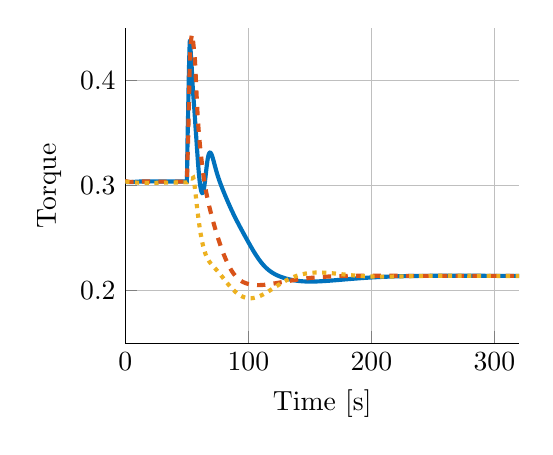
\begin{tikzpicture}

\begin{axis}[%
width=5cm,
height=4cm,
at={(0\linewidth,0\linewidth)},
scale only axis,
xmin=0,
xmax=320,
xlabel={Time [s]},
xmajorgrids,
ymin=0.15,
ymax=0.45,
ylabel={Torque},
ymajorgrids,
axis background/.style={fill=white},
% title style={font=\bfseries},
% title={Normalized Torque Setting},
axis x line*=bottom,
axis y line*=left
]
\addplot [color=mycolor1,solid,line width=1.5pt,forget plot]
  table[row sep=crcr]{%
0	0.30400978288\\
0.25	0.3039140382\\
0.5	0.303898715\\
0.75	0.303849644\\
1	0.303742664\\
1.25	0.303657633\\
1.5	0.303597146\\
1.75	0.303542376\\
2	0.303496532\\
2.25	0.303463798\\
2.5	0.303441868\\
2.75	0.303428301\\
3	0.303421493\\
3.25	0.303419909\\
3.5	0.303421717\\
3.75	0.30342511\\
4	0.303428553\\
4.25	0.303431526\\
4.5	0.303434849\\
4.75	0.303440032\\
5	0.303448488\\
5.25	0.303461125\\
5.5	0.303478337\\
5.75	0.30349989\\
6	0.303524847\\
6.25	0.303551716\\
6.5	0.303578744\\
6.75	0.303604316\\
7	0.303627354\\
7.25	0.303647554\\
7.5	0.303665378\\
7.75	0.30368185\\
8	0.303698259\\
8.25	0.303715821\\
8.5	0.303735369\\
8.75	0.303757135\\
9	0.303780689\\
9.25	0.303805038\\
9.5	0.303828878\\
9.75	0.303850919\\
10	0.3038702\\
10.25	0.303886312\\
10.5	0.303899485\\
10.75	0.3039105018\\
11	0.3039204969\\
11.25	0.3039306579\\
11.5	0.3039419314\\
11.75	0.3039547915\\
12	0.303969133\\
12.25	0.303984311\\
12.5	0.303999316205\\
12.75	0.3040130387\\
13	0.3040245537\\
13.25	0.3040333552\\
13.5	0.304039481\\
13.75	0.3040434978\\
14	0.3040463533\\
14.25	0.304049135\\
14.5	0.3040527985\\
14.75	0.3040579343\\
15	0.3040646292\\
15.25	0.3040724572\\
15.5	0.3040805989\\
15.75	0.3040880599\\
16	0.3040939305\\
16.25	0.3040976215\\
16.5	0.3040990151\\
16.75	0.3040984935\\
17	0.3040968393\\
17.25	0.3040950349\\
17.5	0.3040940141\\
17.75	0.3040944288\\
18	0.3040964899\\
18.25	0.304099921\\
18.5	0.304104037\\
18.75	0.304107926\\
19	0.304110689\\
19.25	0.304111672\\
19.5	0.304110637\\
19.75	0.304107823\\
20	0.304103883\\
20.25	0.304099714\\
20.5	0.3040962284\\
20.75	0.3040941214\\
21	0.3040936953\\
21.25	0.3040947862\\
21.5	0.3040968102\\
21.75	0.304098917\\
22	0.304100213\\
22.25	0.3040999938\\
22.5	0.3040979296\\
22.75	0.3040941496\\
23	0.304089209\\
23.25	0.3040839448\\
23.5	0.3040792588\\
23.75	0.3040758855\\
24	0.304074203\\
24.25	0.3040741366\\
24.5	0.3040751794\\
24.75	0.3040765248\\
25	0.3040772772\\
25.25	0.3040766871\\
25.5	0.304074348\\
25.75	0.3040703036\\
26	0.304065038\\
26.25	0.3040593495\\
26.5	0.3040541434\\
26.75	0.3040501962\\
27	0.3040479541\\
27.25	0.3040474154\\
27.5	0.3040481308\\
27.75	0.3040493193\\
28	0.304050072\\
28.25	0.3040495916\\
28.5	0.3040474025\\
28.75	0.3040434789\\
29	0.3040382535\\
29.25	0.3040325059\\
29.5	0.3040271596\\
29.75	0.3040230404\\
30	0.3040206593\\
30.25	0.304020077\\
30.5	0.3040208847\\
30.75	0.3040223088\\
31	0.3040234127\\
31.25	0.304023343\\
31.5	0.3040215568\\
31.75	0.3040179687\\
32	0.3040129764\\
32.25	0.30400736019\\
32.5	0.30400207849\\
32.75	0.30399801671\\
33	0.30399575263\\
33.25	0.30399540111\\
33.5	0.30399657907\\
33.75	0.30399850171\\
34	0.304000186395\\
34.25	0.304000711878\\
34.5	0.303999464688\\
34.75	0.30399630629\\
35	0.30399161524\\
35.25	0.3039861918\\
35.5	0.3039810494\\
35.75	0.3039771474\\
36	0.3039751358\\
36.25	0.3039751785\\
36.5	0.3039769034\\
36.75	0.3039794935\\
37	0.3039818991\\
37.25	0.3039831145\\
37.5	0.3039824489\\
37.75	0.3039797154\\
38	0.3039752887\\
38.25	0.3039700121\\
38.5	0.3039649776\\
38.75	0.3039612378\\
39	0.3039595238\\
39.25	0.3039600447\\
39.5	0.3039624233\\
39.75	0.3039657865\\
40	0.3039689909\\
40.25	0.3039709253\\
40.5	0.3039708108\\
40.75	0.3039684163\\
41	0.3039641305\\
41.25	0.3039588667\\
41.5	0.3039538256\\
41.75	0.3039501775\\
42	0.3039487466\\
42.25	0.3039497841\\
42.5	0.3039528884\\
42.75	0.3039571003\\
43	0.3039611496\\
43.25	0.3039637918\\
43.5	0.3039641463\\
43.75	0.3039619421\\
44	0.3039576037\\
44.25	0.3039521491\\
44.5	0.3039469257\\
44.75	0.3039432525\\
45	0.3039420629\\
45.25	0.303943645\\
45.5	0.3039475487\\
45.75	0.3039526896\\
46	0.3039576277\\
46.25	0.3039609501\\
46.5	0.3039616569\\
46.75	0.3039594436\\
47	0.3039548\\
47.25	0.3039488939\\
47.5	0.3039432685\\
47.75	0.303939431\\
48	0.3039384434\\
48.25	0.303940623\\
48.5	0.303945437\\
48.75	0.3039516243\\
49	0.3039575187\\
49.25	0.303961494\\
49.5	0.3039624102\\
49.75	0.3039599403\\
50	0.3039546798\\
50.25	0.3171159\\
50.5	0.3392608\\
50.75	0.3547082\\
51	0.3663522\\
51.25	0.3827232\\
51.5	0.3991287\\
51.75	0.411846\\
52	0.423182\\
52.25	0.433125\\
52.5	0.439159\\
52.75	0.43593\\
53	0.429983\\
53.25	0.425146\\
53.5	0.421035\\
53.75	0.416763\\
54	0.411641\\
54.25	0.405724\\
54.5	0.3999344\\
54.75	0.3949111\\
55	0.3904759\\
55.25	0.3862206\\
55.5	0.3820063\\
55.75	0.3780323\\
56	0.3742622\\
56.25	0.3701397\\
56.5	0.3657399\\
56.75	0.3613966\\
57	0.3571217\\
57.25	0.352845\\
57.5	0.3485722\\
57.75	0.3443044\\
58	0.3400287\\
58.25	0.3357414\\
58.5	0.3314702\\
58.75	0.3272726\\
59	0.323204\\
59.25	0.3193062\\
59.5	0.3156146\\
59.75	0.31215964\\
60	0.30896388\\
60.25	0.30604294\\
60.5	0.303407557\\
60.75	0.30106472\\
61	0.29901842\\
61.25	0.29727064\\
61.5	0.29582245\\
61.75	0.29467478\\
62	0.2938289\\
62.25	0.2932867\\
62.5	0.2930506\\
62.75	0.293123\\
63	0.2935058\\
63.25	0.29419939\\
63.5	0.29520118\\
63.75	0.29650428\\
64	0.29809599\\
64.25	0.29995649\\
64.5	0.30205794\\
64.75	0.304364273\\
65	0.30683158\\
65.25	0.30940915\\
65.5	0.31204077\\
65.75	0.3146662\\
66	0.3172236\\
66.25	0.3196532\\
66.5	0.3219038\\
66.75	0.3239373\\
67	0.325731\\
67.25	0.3272746\\
67.5	0.3285669\\
67.75	0.3296131\\
68	0.330422\\
68.25	0.331005\\
68.5	0.331375\\
68.75	0.331546\\
69	0.3315327\\
69.25	0.3313504\\
69.5	0.3310144\\
69.75	0.3305404\\
70	0.329944\\
70.25	0.3292405\\
70.5	0.3284447\\
70.75	0.3275709\\
71	0.3266324\\
71.25	0.3256419\\
71.5	0.3246109\\
71.75	0.3235498\\
72	0.3224681\\
72.25	0.3213741\\
72.5	0.3202748\\
72.75	0.3191767\\
73	0.3180848\\
73.25	0.3170035\\
73.5	0.3159362\\
73.75	0.3148855\\
74	0.31385345\\
74.25	0.31284136\\
74.5	0.31185003\\
74.75	0.3108798\\
75	0.30993062\\
75.25	0.30900211\\
75.5	0.30809362\\
75.75	0.3072043\\
76	0.30633316\\
76.25	0.30547909\\
76.5	0.304640912\\
76.75	0.303817421\\
77	0.303007412\\
77.25	0.3022097\\
77.5	0.30142315\\
77.75	0.30064668\\
78	0.29987927\\
78.25	0.29912001\\
78.5	0.29836803\\
78.75	0.29762258\\
79	0.296883\\
79.25	0.29614868\\
79.5	0.29541912\\
79.75	0.29469391\\
80	0.2939727\\
80.25	0.2932552\\
80.5	0.2925411\\
80.75	0.2918304\\
81	0.2911229\\
81.25	0.2904185\\
81.5	0.2897172\\
81.75	0.2890189\\
82	0.2883238\\
82.25	0.2876317\\
82.5	0.2869429\\
82.75	0.2862573\\
83	0.285575\\
83.25	0.2848961\\
83.5	0.2842207\\
83.75	0.2835488\\
84	0.2828806\\
84.25	0.282216\\
84.5	0.2815552\\
84.75	0.2808982\\
85	0.2802451\\
85.25	0.2795958\\
85.5	0.2789505\\
85.75	0.2783091\\
86	0.2776717\\
86.25	0.2770383\\
86.5	0.2764088\\
86.75	0.2757832\\
87	0.2751616\\
87.25	0.2745438\\
87.5	0.2739299\\
87.75	0.2733197\\
88	0.2727133\\
88.25	0.2721105\\
88.5	0.2715114\\
88.75	0.2709157\\
89	0.2703235\\
89.25	0.2697346\\
89.5	0.269149\\
89.75	0.2685665\\
90	0.2679871\\
90.25	0.2674107\\
90.5	0.2668371\\
90.75	0.2662662\\
91	0.2656979\\
91.25	0.2651322\\
91.5	0.2645689\\
91.75	0.2640079\\
92	0.263449\\
92.25	0.2628923\\
92.5	0.2623375\\
92.75	0.2617845\\
93	0.2612333\\
93.25	0.2606838\\
93.5	0.2601357\\
93.75	0.2595892\\
94	0.259044\\
94.25	0.2585\\
94.5	0.2579573\\
94.75	0.2574156\\
95	0.256875\\
95.25	0.2563354\\
95.5	0.2557967\\
95.75	0.2552589\\
96	0.2547219\\
96.25	0.2541856\\
96.5	0.2536501\\
96.75	0.2531154\\
97	0.2525813\\
97.25	0.252048\\
97.5	0.2515154\\
97.75	0.2509835\\
98	0.2504523\\
98.25	0.2499219\\
98.5	0.2493923\\
98.75	0.2488635\\
99	0.2483356\\
99.25	0.2478087\\
99.5	0.2472827\\
99.75	0.2467579\\
100	0.2462342\\
100.25	0.2457117\\
100.5	0.2451906\\
100.75	0.2446709\\
101	0.2441528\\
101.25	0.2436363\\
101.5	0.2431215\\
101.75	0.2426087\\
102	0.2420978\\
102.25	0.2415891\\
102.5	0.2410826\\
102.75	0.2405785\\
103	0.2400769\\
103.25	0.239578\\
103.5	0.2390819\\
103.75	0.2385887\\
104	0.2380986\\
104.25	0.2376118\\
104.5	0.2371282\\
104.75	0.2366482\\
105	0.2361718\\
105.25	0.2356992\\
105.5	0.2352304\\
105.75	0.2347657\\
106	0.2343052\\
106.25	0.2338489\\
106.5	0.2333971\\
106.75	0.2329498\\
107	0.2325071\\
107.25	0.2320691\\
107.5	0.231636\\
107.75	0.2312078\\
108	0.2307847\\
108.25	0.2303667\\
108.5	0.2299539\\
108.75	0.2295464\\
109	0.2291442\\
109.25	0.2287474\\
109.5	0.2283561\\
109.75	0.2279704\\
110	0.2275902\\
110.25	0.2272156\\
110.5	0.2268466\\
110.75	0.2264833\\
111	0.2261257\\
111.25	0.2257738\\
111.5	0.2254276\\
111.75	0.2250872\\
112	0.2247524\\
112.25	0.2244233\\
112.5	0.2240999\\
112.75	0.2237821\\
113	0.22347\\
113.25	0.2231635\\
113.5	0.2228625\\
113.75	0.2225671\\
114	0.2222772\\
114.25	0.2219927\\
114.5	0.2217135\\
114.75	0.2214397\\
115	0.2211711\\
115.25	0.2209078\\
115.5	0.2206495\\
115.75	0.2203964\\
116	0.2201482\\
116.25	0.2199049\\
116.5	0.2196664\\
116.75	0.2194328\\
117	0.2192037\\
117.25	0.2189793\\
117.5	0.2187594\\
117.75	0.2185439\\
118	0.2183328\\
118.25	0.2181259\\
118.5	0.2179231\\
118.75	0.2177245\\
119	0.2175298\\
119.25	0.2173391\\
119.5	0.2171522\\
119.75	0.216969\\
120	0.2167894\\
120.25	0.2166135\\
120.5	0.216441\\
120.75	0.2162719\\
121	0.2161061\\
121.25	0.2159436\\
121.5	0.2157842\\
121.75	0.215628\\
122	0.2154747\\
122.25	0.2153244\\
122.5	0.2151769\\
122.75	0.2150322\\
123	0.2148902\\
123.25	0.2147509\\
123.5	0.2146142\\
123.75	0.2144799\\
124	0.2143482\\
124.25	0.2142188\\
124.5	0.2140918\\
124.75	0.2139671\\
125	0.2138446\\
125.25	0.2137242\\
125.5	0.213606\\
125.75	0.2134899\\
126	0.2133758\\
126.25	0.2132637\\
126.5	0.2131536\\
126.75	0.2130453\\
127	0.2129389\\
127.25	0.2128343\\
127.5	0.2127315\\
127.75	0.2126304\\
128	0.2125311\\
128.25	0.2124334\\
128.5	0.2123374\\
128.75	0.212243\\
129	0.2121502\\
129.25	0.212059\\
129.5	0.2119693\\
129.75	0.2118812\\
130	0.2117945\\
130.25	0.2117093\\
130.5	0.2116256\\
130.75	0.2115433\\
131	0.2114624\\
131.25	0.211383\\
131.5	0.2113049\\
131.75	0.2112282\\
132	0.2111528\\
132.25	0.2110788\\
132.5	0.2110061\\
132.75	0.2109348\\
133	0.2108647\\
133.25	0.210796\\
133.5	0.2107285\\
133.75	0.2106623\\
134	0.2105973\\
134.25	0.2105336\\
134.5	0.2104712\\
134.75	0.2104099\\
135	0.2103499\\
135.25	0.2102912\\
135.5	0.2102336\\
135.75	0.2101772\\
136	0.2101221\\
136.25	0.2100681\\
136.5	0.2100153\\
136.75	0.2099637\\
137	0.2099132\\
137.25	0.2098639\\
137.5	0.2098157\\
137.75	0.2097687\\
138	0.2097229\\
138.25	0.2096781\\
138.5	0.2096345\\
138.75	0.209592\\
139	0.2095506\\
139.25	0.2095103\\
139.5	0.2094711\\
139.75	0.209433\\
140	0.2093959\\
140.25	0.20936\\
140.5	0.209325\\
140.75	0.2092912\\
141	0.2092584\\
141.25	0.2092266\\
141.5	0.2091959\\
141.75	0.2091661\\
142	0.2091374\\
142.25	0.2091097\\
142.5	0.209083\\
142.75	0.2090573\\
143	0.2090325\\
143.25	0.2090087\\
143.5	0.2089859\\
143.75	0.208964\\
144	0.208943\\
144.25	0.208923\\
144.5	0.2089038\\
144.75	0.2088856\\
145	0.2088683\\
145.25	0.2088519\\
145.5	0.2088363\\
145.75	0.2088216\\
146	0.2088077\\
146.25	0.2087947\\
146.5	0.2087825\\
146.75	0.2087712\\
147	0.2087606\\
147.25	0.2087508\\
147.5	0.2087419\\
147.75	0.2087336\\
148	0.2087262\\
148.25	0.2087195\\
148.5	0.2087136\\
148.75	0.2087083\\
149	0.2087038\\
149.25	0.2087\\
149.5	0.2086969\\
149.75	0.2086945\\
150	0.2086927\\
150.25	0.2086917\\
150.5	0.2086912\\
150.75	0.2086914\\
151	0.2086922\\
151.25	0.2086937\\
151.5	0.2086957\\
151.75	0.2086984\\
152	0.2087016\\
152.25	0.2087054\\
152.5	0.2087098\\
152.75	0.2087147\\
153	0.2087202\\
153.25	0.2087262\\
153.5	0.2087327\\
153.75	0.2087397\\
154	0.2087472\\
154.25	0.2087552\\
154.5	0.2087637\\
154.75	0.2087727\\
155	0.2087821\\
155.25	0.208792\\
155.5	0.2088023\\
155.75	0.2088131\\
156	0.2088243\\
156.25	0.2088359\\
156.5	0.2088479\\
156.75	0.2088603\\
157	0.2088731\\
157.25	0.2088863\\
157.5	0.2088998\\
157.75	0.2089137\\
158	0.208928\\
158.25	0.2089426\\
158.5	0.2089576\\
158.75	0.2089729\\
159	0.2089885\\
159.25	0.2090044\\
159.5	0.2090206\\
159.75	0.2090372\\
160	0.209054\\
160.25	0.2090711\\
160.5	0.2090885\\
160.75	0.2091062\\
161	0.2091242\\
161.25	0.2091424\\
161.5	0.2091608\\
161.75	0.2091795\\
162	0.2091985\\
162.25	0.2092177\\
162.5	0.2092371\\
162.75	0.2092567\\
163	0.2092765\\
163.25	0.2092966\\
163.5	0.2093169\\
163.75	0.2093373\\
164	0.209358\\
164.25	0.2093788\\
164.5	0.2093999\\
164.75	0.2094211\\
165	0.2094425\\
165.25	0.209464\\
165.5	0.2094857\\
165.75	0.2095076\\
166	0.2095296\\
166.25	0.2095518\\
166.5	0.2095741\\
166.75	0.2095965\\
167	0.2096191\\
167.25	0.2096418\\
167.5	0.2096646\\
167.75	0.2096876\\
168	0.2097107\\
168.25	0.2097339\\
168.5	0.2097571\\
168.75	0.2097805\\
169	0.209804\\
169.25	0.2098276\\
169.5	0.2098513\\
169.75	0.2098751\\
170	0.2098989\\
170.25	0.2099229\\
170.5	0.2099469\\
170.75	0.2099709\\
171	0.2099951\\
171.25	0.2100193\\
171.5	0.2100436\\
171.75	0.2100679\\
172	0.2100923\\
172.25	0.2101167\\
172.5	0.2101412\\
172.75	0.2101658\\
173	0.2101903\\
173.25	0.2102149\\
173.5	0.2102396\\
173.75	0.2102643\\
174	0.210289\\
174.25	0.2103137\\
174.5	0.2103385\\
174.75	0.2103632\\
175	0.210388\\
175.25	0.2104128\\
175.5	0.2104377\\
175.75	0.2104625\\
176	0.2104873\\
176.25	0.2105121\\
176.5	0.210537\\
176.75	0.2105618\\
177	0.2105866\\
177.25	0.2106115\\
177.5	0.2106363\\
177.75	0.2106611\\
178	0.2106858\\
178.25	0.2107106\\
178.5	0.2107353\\
178.75	0.2107601\\
179	0.2107848\\
179.25	0.2108094\\
179.5	0.2108341\\
179.75	0.2108587\\
180	0.2108832\\
180.25	0.2109078\\
180.5	0.2109323\\
180.75	0.2109567\\
181	0.2109812\\
181.25	0.2110055\\
181.5	0.2110299\\
181.75	0.2110541\\
182	0.2110784\\
182.25	0.2111025\\
182.5	0.2111267\\
182.75	0.2111507\\
183	0.2111747\\
183.25	0.2111987\\
183.5	0.2112226\\
183.75	0.2112464\\
184	0.2112702\\
184.25	0.2112939\\
184.5	0.2113175\\
184.75	0.2113411\\
185	0.2113646\\
185.25	0.211388\\
185.5	0.2114113\\
185.75	0.2114346\\
186	0.2114578\\
186.25	0.2114809\\
186.5	0.2115039\\
186.75	0.2115269\\
187	0.2115498\\
187.25	0.2115726\\
187.5	0.2115953\\
187.75	0.2116179\\
188	0.2116404\\
188.25	0.2116629\\
188.5	0.2116852\\
188.75	0.2117075\\
189	0.2117297\\
189.25	0.2117518\\
189.5	0.2117738\\
189.75	0.2117957\\
190	0.2118175\\
190.25	0.2118392\\
190.5	0.2118608\\
190.75	0.2118823\\
191	0.2119037\\
191.25	0.211925\\
191.5	0.2119462\\
191.75	0.2119674\\
192	0.2119884\\
192.25	0.2120093\\
192.5	0.2120301\\
192.75	0.2120508\\
193	0.2120714\\
193.25	0.2120919\\
193.5	0.2121123\\
193.75	0.2121325\\
194	0.2121527\\
194.25	0.2121728\\
194.5	0.2121927\\
194.75	0.2122126\\
195	0.2122323\\
195.25	0.212252\\
195.5	0.2122715\\
195.75	0.2122909\\
196	0.2123102\\
196.25	0.2123294\\
196.5	0.2123485\\
196.75	0.2123674\\
197	0.2123863\\
197.25	0.212405\\
197.5	0.2124236\\
197.75	0.2124421\\
198	0.2124605\\
198.25	0.2124788\\
198.5	0.212497\\
198.75	0.2125151\\
199	0.212533\\
199.25	0.2125508\\
199.5	0.2125685\\
199.75	0.2125861\\
200	0.2126036\\
200.25	0.212621\\
200.5	0.2126382\\
200.75	0.2126554\\
201	0.2126724\\
201.25	0.2126893\\
201.5	0.2127061\\
201.75	0.2127228\\
202	0.2127393\\
202.25	0.2127558\\
202.5	0.2127721\\
202.75	0.2127883\\
203	0.2128044\\
203.25	0.2128204\\
203.5	0.2128363\\
203.75	0.212852\\
204	0.2128676\\
204.25	0.2128832\\
204.5	0.2128986\\
204.75	0.2129139\\
205	0.212929\\
205.25	0.2129441\\
205.5	0.212959\\
205.75	0.2129739\\
206	0.2129886\\
206.25	0.2130032\\
206.5	0.2130177\\
206.75	0.213032\\
207	0.2130463\\
207.25	0.2130605\\
207.5	0.2130745\\
207.75	0.2130884\\
208	0.2131022\\
208.25	0.2131159\\
208.5	0.2131295\\
208.75	0.213143\\
209	0.2131563\\
209.25	0.2131696\\
209.5	0.2131827\\
209.75	0.2131957\\
210	0.2132087\\
210.25	0.2132215\\
210.5	0.2132342\\
210.75	0.2132468\\
211	0.2132592\\
211.25	0.2132716\\
211.5	0.2132839\\
211.75	0.213296\\
212	0.2133081\\
212.25	0.21332\\
212.5	0.2133318\\
212.75	0.2133436\\
213	0.2133552\\
213.25	0.2133667\\
213.5	0.2133781\\
213.75	0.2133894\\
214	0.2134006\\
214.25	0.2134117\\
214.5	0.2134227\\
214.75	0.2134336\\
215	0.2134443\\
215.25	0.213455\\
215.5	0.2134656\\
215.75	0.2134761\\
216	0.2134865\\
216.25	0.2134967\\
216.5	0.2135069\\
216.75	0.213517\\
217	0.213527\\
217.25	0.2135368\\
217.5	0.2135466\\
217.75	0.2135563\\
218	0.2135659\\
218.25	0.2135754\\
218.5	0.2135847\\
218.75	0.213594\\
219	0.2136032\\
219.25	0.2136123\\
219.5	0.2136213\\
219.75	0.2136303\\
220	0.2136391\\
220.25	0.2136478\\
220.5	0.2136564\\
220.75	0.213665\\
221	0.2136734\\
221.25	0.2136818\\
221.5	0.2136901\\
221.75	0.2136983\\
222	0.2137063\\
222.25	0.2137144\\
222.5	0.2137223\\
222.75	0.2137301\\
223	0.2137378\\
223.25	0.2137455\\
223.5	0.213753\\
223.75	0.2137605\\
224	0.2137679\\
224.25	0.2137752\\
224.5	0.2137825\\
224.75	0.2137896\\
225	0.2137967\\
225.25	0.2138036\\
225.5	0.2138105\\
225.75	0.2138173\\
226	0.2138241\\
226.25	0.2138307\\
226.5	0.2138373\\
226.75	0.2138438\\
227	0.2138502\\
227.25	0.2138565\\
227.5	0.2138628\\
227.75	0.213869\\
228	0.2138751\\
228.25	0.2138811\\
228.5	0.2138871\\
228.75	0.213893\\
229	0.2138988\\
229.25	0.2139045\\
229.5	0.2139101\\
229.75	0.2139157\\
230	0.2139212\\
230.25	0.2139267\\
230.5	0.2139321\\
230.75	0.2139374\\
231	0.2139426\\
231.25	0.2139477\\
231.5	0.2139528\\
231.75	0.2139579\\
232	0.2139628\\
232.25	0.2139677\\
232.5	0.2139725\\
232.75	0.2139773\\
233	0.213982\\
233.25	0.2139866\\
233.5	0.2139911\\
233.75	0.2139956\\
234	0.2140001\\
234.25	0.2140044\\
234.5	0.2140087\\
234.75	0.214013\\
235	0.2140171\\
235.25	0.2140213\\
235.5	0.2140253\\
235.75	0.2140293\\
236	0.2140333\\
236.25	0.2140371\\
236.5	0.214041\\
236.75	0.2140447\\
237	0.2140484\\
237.25	0.2140521\\
237.5	0.2140557\\
237.75	0.2140592\\
238	0.2140627\\
238.25	0.2140661\\
238.5	0.2140695\\
238.75	0.2140728\\
239	0.2140761\\
239.25	0.2140793\\
239.5	0.2140824\\
239.75	0.2140856\\
240	0.2140886\\
240.25	0.2140916\\
240.5	0.2140946\\
240.75	0.2140975\\
241	0.2141003\\
241.25	0.2141031\\
241.5	0.2141059\\
241.75	0.2141086\\
242	0.2141113\\
242.25	0.2141139\\
242.5	0.2141164\\
242.75	0.214119\\
243	0.2141214\\
243.25	0.2141239\\
243.5	0.2141263\\
243.75	0.2141286\\
244	0.2141309\\
244.25	0.2141332\\
244.5	0.2141354\\
244.75	0.2141375\\
245	0.2141397\\
245.25	0.2141417\\
245.5	0.2141438\\
245.75	0.2141458\\
246	0.2141478\\
246.25	0.2141497\\
246.5	0.2141516\\
246.75	0.2141534\\
247	0.2141552\\
247.25	0.214157\\
247.5	0.2141587\\
247.75	0.2141604\\
248	0.2141621\\
248.25	0.2141637\\
248.5	0.2141653\\
248.75	0.2141668\\
249	0.2141683\\
249.25	0.2141698\\
249.5	0.2141712\\
249.75	0.2141726\\
250	0.214174\\
250.25	0.2141753\\
250.5	0.2141767\\
250.75	0.2141779\\
251	0.2141792\\
251.25	0.2141804\\
251.5	0.2141816\\
251.75	0.2141827\\
252	0.2141838\\
252.25	0.2141849\\
252.5	0.214186\\
252.75	0.214187\\
253	0.214188\\
253.25	0.214189\\
253.5	0.2141899\\
253.75	0.2141908\\
254	0.2141917\\
254.25	0.2141926\\
254.5	0.2141934\\
254.75	0.2141942\\
255	0.214195\\
255.25	0.2141957\\
255.5	0.2141965\\
255.75	0.2141972\\
256	0.2141978\\
256.25	0.2141985\\
256.5	0.2141991\\
256.75	0.2141997\\
257	0.2142003\\
257.25	0.2142008\\
257.5	0.2142014\\
257.75	0.2142019\\
258	0.2142024\\
258.25	0.2142028\\
258.5	0.2142033\\
258.75	0.2142037\\
259	0.2142041\\
259.25	0.2142045\\
259.5	0.2142048\\
259.75	0.2142052\\
260	0.2142055\\
260.25	0.2142058\\
260.5	0.2142061\\
260.75	0.2142063\\
261	0.2142066\\
261.25	0.2142068\\
261.5	0.214207\\
261.75	0.2142072\\
262	0.2142074\\
262.25	0.2142075\\
262.5	0.2142077\\
262.75	0.2142078\\
263	0.2142079\\
263.25	0.214208\\
263.5	0.214208\\
263.75	0.2142081\\
264	0.2142081\\
264.25	0.2142081\\
264.5	0.2142081\\
264.75	0.2142081\\
265	0.2142081\\
265.25	0.2142081\\
265.5	0.214208\\
265.75	0.2142079\\
266	0.2142079\\
266.25	0.2142078\\
266.5	0.2142077\\
266.75	0.2142075\\
267	0.2142074\\
267.25	0.2142073\\
267.5	0.2142071\\
267.75	0.2142069\\
268	0.2142068\\
268.25	0.2142066\\
268.5	0.2142064\\
268.75	0.2142061\\
269	0.2142059\\
269.25	0.2142057\\
269.5	0.2142054\\
269.75	0.2142052\\
270	0.2142049\\
270.25	0.2142046\\
270.5	0.2142043\\
270.75	0.214204\\
271	0.2142037\\
271.25	0.2142034\\
271.5	0.2142031\\
271.75	0.2142028\\
272	0.2142024\\
272.25	0.2142021\\
272.5	0.2142017\\
272.75	0.2142013\\
273	0.214201\\
273.25	0.2142006\\
273.5	0.2142002\\
273.75	0.2141998\\
274	0.2141994\\
274.25	0.214199\\
274.5	0.2141985\\
274.75	0.2141981\\
275	0.2141977\\
275.25	0.2141972\\
275.5	0.2141968\\
275.75	0.2141963\\
276	0.2141959\\
276.25	0.2141954\\
276.5	0.2141949\\
276.75	0.2141945\\
277	0.214194\\
277.25	0.2141935\\
277.5	0.214193\\
277.75	0.2141925\\
278	0.214192\\
278.25	0.2141915\\
278.5	0.214191\\
278.75	0.2141905\\
279	0.21419\\
279.25	0.2141894\\
279.5	0.2141889\\
279.75	0.2141884\\
280	0.2141878\\
280.25	0.2141873\\
280.5	0.2141868\\
280.75	0.2141862\\
281	0.2141857\\
281.25	0.2141851\\
281.5	0.2141845\\
281.75	0.214184\\
282	0.2141834\\
282.25	0.2141829\\
282.5	0.2141823\\
282.75	0.2141817\\
283	0.2141812\\
283.25	0.2141806\\
283.5	0.21418\\
283.75	0.2141794\\
284	0.2141788\\
284.25	0.2141783\\
284.5	0.2141777\\
284.75	0.2141771\\
285	0.2141765\\
285.25	0.2141759\\
285.5	0.2141753\\
285.75	0.2141747\\
286	0.2141741\\
286.25	0.2141736\\
286.5	0.214173\\
286.75	0.2141724\\
287	0.2141718\\
287.25	0.2141712\\
287.5	0.2141706\\
287.75	0.21417\\
288	0.2141694\\
288.25	0.2141688\\
288.5	0.2141682\\
288.75	0.2141676\\
289	0.214167\\
289.25	0.2141664\\
289.5	0.2141658\\
289.75	0.2141652\\
290	0.2141646\\
290.25	0.214164\\
290.5	0.2141634\\
290.75	0.2141628\\
291	0.2141622\\
291.25	0.2141616\\
291.5	0.214161\\
291.75	0.2141604\\
292	0.2141598\\
292.25	0.2141592\\
292.5	0.2141586\\
292.75	0.214158\\
293	0.2141574\\
293.25	0.2141568\\
293.5	0.2141562\\
293.75	0.2141556\\
294	0.214155\\
294.25	0.2141544\\
294.5	0.2141538\\
294.75	0.2141532\\
295	0.2141527\\
295.25	0.2141521\\
295.5	0.2141515\\
295.75	0.2141509\\
296	0.2141503\\
296.25	0.2141497\\
296.5	0.2141492\\
296.75	0.2141486\\
297	0.214148\\
297.25	0.2141474\\
297.5	0.2141469\\
297.75	0.2141463\\
298	0.2141457\\
298.25	0.2141452\\
298.5	0.2141446\\
298.75	0.214144\\
299	0.2141435\\
299.25	0.2141429\\
299.5	0.2141424\\
299.75	0.2141418\\
300	0.2141413\\
300.25	0.2141407\\
300.5	0.2141402\\
300.75	0.2141396\\
301	0.2141391\\
301.25	0.2141385\\
301.5	0.214138\\
301.75	0.2141374\\
302	0.2141369\\
302.25	0.2141364\\
302.5	0.2141358\\
302.75	0.2141353\\
303	0.2141348\\
303.25	0.2141343\\
303.5	0.2141337\\
303.75	0.2141332\\
304	0.2141327\\
304.25	0.2141322\\
304.5	0.2141317\\
304.75	0.2141312\\
305	0.2141307\\
305.25	0.2141302\\
305.5	0.2141297\\
305.75	0.2141292\\
306	0.2141287\\
306.25	0.2141282\\
306.5	0.2141277\\
306.75	0.2141272\\
307	0.2141267\\
307.25	0.2141262\\
307.5	0.2141257\\
307.75	0.2141253\\
308	0.2141248\\
308.25	0.2141243\\
308.5	0.2141238\\
308.75	0.2141234\\
309	0.2141229\\
309.25	0.2141224\\
309.5	0.214122\\
309.75	0.2141215\\
310	0.2141211\\
310.25	0.2141206\\
310.5	0.2141202\\
310.75	0.2141197\\
311	0.2141193\\
311.25	0.2141189\\
311.5	0.2141184\\
311.75	0.214118\\
312	0.2141175\\
312.25	0.2141171\\
312.5	0.2141167\\
312.75	0.2141163\\
313	0.2141159\\
313.25	0.2141154\\
313.5	0.214115\\
313.75	0.2141146\\
314	0.2141142\\
314.25	0.2141138\\
314.5	0.2141134\\
314.75	0.214113\\
315	0.2141126\\
315.25	0.2141122\\
315.5	0.2141118\\
315.75	0.2141114\\
316	0.214111\\
316.25	0.2141107\\
316.5	0.2141103\\
316.75	0.2141099\\
317	0.2141095\\
317.25	0.2141091\\
317.5	0.2141088\\
317.75	0.2141084\\
318	0.2141081\\
318.25	0.2141077\\
318.5	0.2141073\\
318.75	0.214107\\
319	0.2141066\\
319.25	0.2141063\\
319.5	0.2141059\\
319.75	0.2141056\\
320	0.2141052\\
320.25	0.2141049\\
320.5	0.2141046\\
320.75	0.2141042\\
321	0.2141039\\
321.25	0.2141036\\
321.5	0.2141033\\
321.75	0.2141029\\
322	0.2141026\\
322.25	0.2141023\\
322.5	0.214102\\
322.75	0.2141017\\
323	0.2141014\\
323.25	0.2141011\\
323.5	0.2141008\\
323.75	0.2141005\\
324	0.2141002\\
324.25	0.2140999\\
324.5	0.2140996\\
324.75	0.2140993\\
325	0.214099\\
325.25	0.2140987\\
325.5	0.2140984\\
325.75	0.2140982\\
326	0.2140979\\
326.25	0.2140976\\
326.5	0.2140973\\
326.75	0.2140971\\
327	0.2140968\\
327.25	0.2140965\\
327.5	0.2140963\\
327.75	0.214096\\
328	0.2140958\\
328.25	0.2140955\\
328.5	0.2140953\\
328.75	0.214095\\
329	0.2140948\\
329.25	0.2140945\\
329.5	0.2140943\\
329.75	0.214094\\
330	0.2140938\\
330.25	0.2140936\\
330.5	0.2140933\\
330.75	0.2140931\\
331	0.2140929\\
331.25	0.2140927\\
331.5	0.2140924\\
331.75	0.2140922\\
332	0.214092\\
332.25	0.2140918\\
332.5	0.2140916\\
332.75	0.2140914\\
333	0.2140911\\
333.25	0.2140909\\
333.5	0.2140907\\
333.75	0.2140905\\
334	0.2140903\\
334.25	0.2140901\\
334.5	0.2140899\\
334.75	0.2140897\\
335	0.2140896\\
335.25	0.2140894\\
335.5	0.2140892\\
335.75	0.214089\\
336	0.2140888\\
336.25	0.2140886\\
336.5	0.2140884\\
336.75	0.2140883\\
337	0.2140881\\
337.25	0.2140879\\
337.5	0.2140878\\
337.75	0.2140876\\
338	0.2140874\\
338.25	0.2140873\\
338.5	0.2140871\\
338.75	0.2140869\\
339	0.2140868\\
339.25	0.2140866\\
339.5	0.2140865\\
339.75	0.2140863\\
340	0.2140862\\
340.25	0.214086\\
340.5	0.2140859\\
340.75	0.2140857\\
341	0.2140856\\
341.25	0.2140854\\
341.5	0.2140853\\
341.75	0.2140852\\
342	0.214085\\
342.25	0.2140849\\
342.5	0.2140848\\
342.75	0.2140846\\
343	0.2140845\\
343.25	0.2140844\\
343.5	0.2140842\\
343.75	0.2140841\\
344	0.214084\\
344.25	0.2140839\\
344.5	0.2140838\\
344.75	0.2140836\\
345	0.2140835\\
345.25	0.2140834\\
345.5	0.2140833\\
345.75	0.2140832\\
346	0.2140831\\
346.25	0.214083\\
346.5	0.2140829\\
346.75	0.2140828\\
347	0.2140826\\
347.25	0.2140825\\
347.5	0.2140824\\
347.75	0.2140823\\
348	0.2140823\\
348.25	0.2140822\\
348.5	0.2140821\\
348.75	0.214082\\
349	0.2140819\\
349.25	0.2140818\\
349.5	0.2140817\\
349.75	0.2140816\\
350	0.2140815\\
350.25	0.2140814\\
350.5	0.2140814\\
350.75	0.2140813\\
351	0.2140812\\
351.25	0.2140811\\
351.5	0.214081\\
351.75	0.214081\\
352	0.2140809\\
352.25	0.2140808\\
352.5	0.2140807\\
352.75	0.2140807\\
353	0.2140806\\
353.25	0.2140805\\
353.5	0.2140805\\
353.75	0.2140804\\
354	0.2140803\\
354.25	0.2140803\\
354.5	0.2140802\\
354.75	0.2140801\\
355	0.2140801\\
355.25	0.21408\\
355.5	0.2140799\\
355.75	0.2140799\\
356	0.2140798\\
356.25	0.2140798\\
356.5	0.2140797\\
356.75	0.2140797\\
357	0.2140796\\
357.25	0.2140796\\
357.5	0.2140795\\
357.75	0.2140795\\
358	0.2140794\\
358.25	0.2140794\\
358.5	0.2140793\\
358.75	0.2140793\\
359	0.2140792\\
359.25	0.2140792\\
359.5	0.2140791\\
359.75	0.2140791\\
360	0.2140791\\
360.25	0.214079\\
360.5	0.214079\\
360.75	0.2140789\\
361	0.2140789\\
361.25	0.2140789\\
361.5	0.2140788\\
361.75	0.2140788\\
362	0.2140788\\
362.25	0.2140787\\
362.5	0.2140787\\
362.75	0.2140787\\
363	0.2140786\\
363.25	0.2140786\\
363.5	0.2140786\\
363.75	0.2140785\\
364	0.2140785\\
364.25	0.2140785\\
364.5	0.2140785\\
364.75	0.2140784\\
365	0.2140784\\
365.25	0.2140784\\
365.5	0.2140784\\
365.75	0.2140783\\
366	0.2140783\\
366.25	0.2140783\\
366.5	0.2140783\\
366.75	0.2140783\\
367	0.2140782\\
367.25	0.2140782\\
367.5	0.2140782\\
367.75	0.2140782\\
368	0.2140782\\
368.25	0.2140782\\
368.5	0.2140781\\
368.75	0.2140781\\
369	0.2140781\\
369.25	0.2140781\\
369.5	0.2140781\\
369.75	0.2140781\\
370	0.2140781\\
370.25	0.214078\\
370.5	0.214078\\
370.75	0.214078\\
371	0.214078\\
371.25	0.214078\\
371.5	0.214078\\
371.75	0.214078\\
372	0.214078\\
372.25	0.214078\\
372.5	0.214078\\
372.75	0.214078\\
373	0.2140779\\
373.25	0.2140779\\
373.5	0.2140779\\
373.75	0.2140779\\
374	0.2140779\\
374.25	0.2140779\\
374.5	0.2140779\\
374.75	0.2140779\\
375	0.2140779\\
375.25	0.2140779\\
375.5	0.2140779\\
375.75	0.2140779\\
376	0.2140779\\
376.25	0.2140779\\
376.5	0.2140779\\
376.75	0.2140779\\
377	0.2140779\\
377.25	0.2140779\\
377.5	0.2140779\\
377.75	0.2140779\\
378	0.2140779\\
378.25	0.2140779\\
378.5	0.2140779\\
378.75	0.2140779\\
379	0.2140779\\
379.25	0.2140779\\
379.5	0.2140779\\
379.75	0.2140779\\
380	0.2140779\\
380.25	0.2140779\\
380.5	0.2140779\\
380.75	0.2140779\\
381	0.214078\\
381.25	0.214078\\
381.5	0.214078\\
381.75	0.214078\\
382	0.214078\\
382.25	0.214078\\
382.5	0.214078\\
382.75	0.214078\\
383	0.214078\\
383.25	0.214078\\
383.5	0.214078\\
383.75	0.214078\\
384	0.214078\\
384.25	0.214078\\
384.5	0.2140781\\
384.75	0.2140781\\
385	0.2140781\\
385.25	0.2140781\\
385.5	0.2140781\\
385.75	0.2140781\\
386	0.2140781\\
386.25	0.2140781\\
386.5	0.2140781\\
386.75	0.2140781\\
387	0.2140782\\
387.25	0.2140782\\
387.5	0.2140782\\
387.75	0.2140782\\
388	0.2140782\\
388.25	0.2140782\\
388.5	0.2140782\\
388.75	0.2140782\\
389	0.2140782\\
389.25	0.2140783\\
389.5	0.2140783\\
389.75	0.2140783\\
390	0.2140783\\
390.25	0.2140783\\
390.5	0.2140783\\
390.75	0.2140783\\
391	0.2140783\\
391.25	0.2140784\\
391.5	0.2140784\\
391.75	0.2140784\\
392	0.2140784\\
392.25	0.2140784\\
392.5	0.2140784\\
392.75	0.2140784\\
393	0.2140784\\
393.25	0.2140785\\
393.5	0.2140785\\
393.75	0.2140785\\
394	0.2140785\\
394.25	0.2140785\\
394.5	0.2140785\\
394.75	0.2140785\\
395	0.2140786\\
395.25	0.2140786\\
395.5	0.2140786\\
395.75	0.2140786\\
396	0.2140786\\
396.25	0.2140786\\
396.5	0.2140786\\
396.75	0.2140787\\
397	0.2140787\\
397.25	0.2140787\\
397.5	0.2140787\\
397.75	0.2140787\\
398	0.2140787\\
398.25	0.2140787\\
398.5	0.2140788\\
398.75	0.2140788\\
399	0.2140788\\
399.25	0.2140788\\
399.5	0.2140788\\
399.75	0.2140788\\
400	0.2140788\\
400.25	0.2140789\\
400.5	0.2140789\\
400.75	0.2140789\\
401	0.2140789\\
401.25	0.2140789\\
401.5	0.2140789\\
401.75	0.2140789\\
402	0.214079\\
402.25	0.214079\\
402.5	0.214079\\
402.75	0.214079\\
403	0.214079\\
403.25	0.214079\\
403.5	0.214079\\
403.75	0.2140791\\
404	0.2140791\\
404.25	0.2140791\\
404.5	0.2140791\\
404.75	0.2140791\\
405	0.2140791\\
405.25	0.2140791\\
405.5	0.2140792\\
405.75	0.2140792\\
406	0.2140792\\
406.25	0.2140792\\
406.5	0.2140792\\
406.75	0.2140792\\
407	0.2140792\\
407.25	0.2140793\\
407.5	0.2140793\\
407.75	0.2140793\\
408	0.2140793\\
408.25	0.2140793\\
408.5	0.2140793\\
408.75	0.2140793\\
409	0.2140794\\
409.25	0.2140794\\
409.5	0.2140794\\
409.75	0.2140794\\
410	0.2140794\\
410.25	0.2140794\\
410.5	0.2140794\\
410.75	0.2140795\\
411	0.2140795\\
411.25	0.2140795\\
411.5	0.2140795\\
411.75	0.2140795\\
412	0.2140795\\
412.25	0.2140795\\
412.5	0.2140796\\
412.75	0.2140796\\
413	0.2140796\\
413.25	0.2140796\\
413.5	0.2140796\\
413.75	0.2140796\\
414	0.2140796\\
414.25	0.2140796\\
414.5	0.2140797\\
414.75	0.2140797\\
415	0.2140797\\
415.25	0.2140797\\
415.5	0.2140797\\
415.75	0.2140797\\
416	0.2140797\\
416.25	0.2140797\\
416.5	0.2140798\\
416.75	0.2140798\\
417	0.2140798\\
417.25	0.2140798\\
417.5	0.2140798\\
417.75	0.2140798\\
418	0.2140798\\
418.25	0.2140798\\
418.5	0.2140799\\
418.75	0.2140799\\
419	0.2140799\\
419.25	0.2140799\\
419.5	0.2140799\\
419.75	0.2140799\\
420	0.2140799\\
420.25	0.2140799\\
420.5	0.21408\\
420.75	0.21408\\
421	0.21408\\
421.25	0.21408\\
421.5	0.21408\\
421.75	0.21408\\
422	0.21408\\
422.25	0.21408\\
422.5	0.21408\\
422.75	0.2140801\\
423	0.2140801\\
423.25	0.2140801\\
423.5	0.2140801\\
423.75	0.2140801\\
424	0.2140801\\
424.25	0.2140801\\
424.5	0.2140801\\
424.75	0.2140801\\
425	0.2140802\\
425.25	0.2140802\\
425.5	0.2140802\\
425.75	0.2140802\\
426	0.2140802\\
426.25	0.2140802\\
426.5	0.2140802\\
426.75	0.2140802\\
427	0.2140802\\
427.25	0.2140802\\
427.5	0.2140802\\
427.75	0.2140803\\
428	0.2140803\\
428.25	0.2140803\\
428.5	0.2140803\\
428.75	0.2140803\\
429	0.2140803\\
429.25	0.2140803\\
429.5	0.2140803\\
429.75	0.2140803\\
430	0.2140803\\
430.25	0.2140804\\
430.5	0.2140804\\
430.75	0.2140804\\
431	0.2140804\\
431.25	0.2140804\\
431.5	0.2140804\\
431.75	0.2140804\\
432	0.2140804\\
432.25	0.2140804\\
432.5	0.2140804\\
432.75	0.2140804\\
433	0.2140804\\
433.25	0.2140805\\
433.5	0.2140805\\
433.75	0.2140805\\
434	0.2140805\\
434.25	0.2140805\\
434.5	0.2140805\\
434.75	0.2140805\\
435	0.2140805\\
435.25	0.2140805\\
435.5	0.2140805\\
435.75	0.2140805\\
436	0.2140805\\
436.25	0.2140805\\
436.5	0.2140806\\
436.75	0.2140806\\
437	0.2140806\\
437.25	0.2140806\\
437.5	0.2140806\\
437.75	0.2140806\\
438	0.2140806\\
438.25	0.2140806\\
438.5	0.2140806\\
438.75	0.2140806\\
439	0.2140806\\
439.25	0.2140806\\
439.5	0.2140806\\
439.75	0.2140806\\
440	0.2140806\\
440.25	0.2140807\\
440.5	0.2140807\\
440.75	0.2140807\\
441	0.2140807\\
441.25	0.2140807\\
441.5	0.2140807\\
441.75	0.2140807\\
442	0.2140807\\
442.25	0.2140807\\
442.5	0.2140807\\
442.75	0.2140807\\
443	0.2140807\\
443.25	0.2140807\\
443.5	0.2140807\\
443.75	0.2140807\\
444	0.2140807\\
444.25	0.2140807\\
444.5	0.2140807\\
444.75	0.2140808\\
445	0.2140808\\
445.25	0.2140808\\
445.5	0.2140808\\
445.75	0.2140808\\
446	0.2140808\\
446.25	0.2140808\\
446.5	0.2140808\\
446.75	0.2140808\\
447	0.2140808\\
447.25	0.2140808\\
447.5	0.2140808\\
447.75	0.2140808\\
448	0.2140808\\
448.25	0.2140808\\
448.5	0.2140808\\
448.75	0.2140808\\
449	0.2140808\\
449.25	0.2140808\\
449.5	0.2140808\\
449.75	0.2140808\\
450	0.2140809\\
450.25	0.2140809\\
450.5	0.2140809\\
450.75	0.2140809\\
451	0.2140809\\
451.25	0.2140809\\
451.5	0.2140809\\
451.75	0.2140809\\
452	0.2140809\\
452.25	0.2140809\\
452.5	0.2140809\\
452.75	0.2140809\\
453	0.2140809\\
453.25	0.2140809\\
453.5	0.2140809\\
453.75	0.2140809\\
454	0.2140809\\
454.25	0.2140809\\
454.5	0.2140809\\
454.75	0.2140809\\
455	0.2140809\\
455.25	0.2140809\\
455.5	0.2140809\\
455.75	0.2140809\\
456	0.2140809\\
456.25	0.2140809\\
456.5	0.2140809\\
456.75	0.2140809\\
457	0.2140809\\
457.25	0.214081\\
457.5	0.214081\\
457.75	0.214081\\
458	0.214081\\
458.25	0.214081\\
458.5	0.214081\\
458.75	0.214081\\
459	0.214081\\
459.25	0.214081\\
459.5	0.214081\\
459.75	0.214081\\
460	0.214081\\
460.25	0.214081\\
460.5	0.214081\\
460.75	0.214081\\
461	0.214081\\
461.25	0.214081\\
461.5	0.214081\\
461.75	0.214081\\
462	0.214081\\
462.25	0.214081\\
462.5	0.214081\\
462.75	0.214081\\
463	0.214081\\
463.25	0.214081\\
463.5	0.214081\\
463.75	0.214081\\
464	0.214081\\
464.25	0.214081\\
464.5	0.214081\\
464.75	0.214081\\
465	0.214081\\
465.25	0.214081\\
465.5	0.214081\\
465.75	0.214081\\
466	0.214081\\
466.25	0.214081\\
466.5	0.214081\\
466.75	0.214081\\
467	0.214081\\
467.25	0.214081\\
467.5	0.214081\\
467.75	0.214081\\
468	0.214081\\
468.25	0.214081\\
468.5	0.214081\\
468.75	0.214081\\
469	0.214081\\
469.25	0.214081\\
469.5	0.214081\\
469.75	0.214081\\
470	0.214081\\
470.25	0.2140811\\
470.5	0.2140811\\
470.75	0.2140811\\
471	0.2140811\\
471.25	0.2140811\\
471.5	0.2140811\\
471.75	0.2140811\\
472	0.2140811\\
472.25	0.2140811\\
472.5	0.2140811\\
472.75	0.2140811\\
473	0.2140811\\
473.25	0.2140811\\
473.5	0.2140811\\
473.75	0.2140811\\
474	0.2140811\\
474.25	0.2140811\\
474.5	0.2140811\\
474.75	0.2140811\\
475	0.2140811\\
475.25	0.2140811\\
475.5	0.2140811\\
475.75	0.2140811\\
476	0.2140811\\
476.25	0.2140811\\
476.5	0.2140811\\
476.75	0.2140811\\
477	0.2140811\\
477.25	0.2140811\\
477.5	0.2140811\\
477.75	0.2140811\\
478	0.2140811\\
478.25	0.2140811\\
478.5	0.2140811\\
478.75	0.2140811\\
479	0.2140811\\
479.25	0.2140811\\
479.5	0.2140811\\
479.75	0.2140811\\
480	0.2140811\\
480.25	0.2140811\\
480.5	0.2140811\\
480.75	0.2140811\\
481	0.2140811\\
481.25	0.2140811\\
481.5	0.2140811\\
481.75	0.2140811\\
482	0.2140811\\
482.25	0.2140811\\
482.5	0.2140811\\
482.75	0.2140811\\
483	0.2140811\\
483.25	0.2140811\\
483.5	0.2140811\\
483.75	0.2140811\\
484	0.2140811\\
484.25	0.2140811\\
484.5	0.2140811\\
484.75	0.2140811\\
485	0.2140811\\
485.25	0.2140811\\
485.5	0.2140811\\
485.75	0.2140811\\
486	0.2140811\\
486.25	0.2140811\\
486.5	0.2140811\\
486.75	0.2140811\\
487	0.2140811\\
487.25	0.2140811\\
487.5	0.2140811\\
487.75	0.2140811\\
488	0.2140811\\
488.25	0.2140811\\
488.5	0.2140811\\
488.75	0.2140811\\
489	0.2140811\\
489.25	0.2140811\\
489.5	0.2140811\\
489.75	0.2140811\\
490	0.2140811\\
490.25	0.2140811\\
490.5	0.2140811\\
490.75	0.2140811\\
491	0.2140811\\
491.25	0.2140811\\
491.5	0.2140811\\
491.75	0.2140811\\
492	0.2140811\\
492.25	0.2140811\\
492.5	0.2140811\\
492.75	0.2140811\\
493	0.2140811\\
493.25	0.2140811\\
493.5	0.2140811\\
493.75	0.2140811\\
494	0.2140811\\
494.25	0.2140811\\
494.5	0.2140811\\
494.75	0.2140811\\
495	0.2140811\\
495.25	0.2140811\\
495.5	0.2140811\\
495.75	0.2140811\\
496	0.2140811\\
496.25	0.2140811\\
496.5	0.2140811\\
496.75	0.2140811\\
497	0.2140811\\
497.25	0.2140811\\
497.5	0.2140811\\
497.75	0.2140811\\
498	0.2140811\\
498.25	0.2140811\\
498.5	0.2140811\\
498.75	0.2140811\\
499	0.2140811\\
499.25	0.2140811\\
499.5	0.2140811\\
499.75	0.2140811\\
};
\addplot [color=mycolor2,dashed,line width=1.5pt,forget plot]
  table[row sep=crcr]{%
0	0.3040175484\\
0.25	0.304105343\\
0.5	0.304222207\\
0.75	0.304199101\\
1	0.304104359\\
1.25	0.3040385347\\
1.5	0.3039892475\\
1.75	0.3039357009\\
2	0.303884439\\
2.25	0.303839439\\
2.5	0.303798192\\
2.75	0.303760292\\
3	0.303726874\\
3.25	0.303698222\\
3.5	0.303674215\\
3.75	0.303654858\\
4	0.303640065\\
4.25	0.303629578\\
4.5	0.30362303\\
4.75	0.303619912\\
5	0.303619629\\
5.25	0.303621608\\
5.5	0.303625367\\
5.75	0.303630534\\
6	0.303636855\\
6.25	0.303644192\\
6.5	0.303652498\\
6.75	0.303661784\\
7	0.303672072\\
7.25	0.303683348\\
7.5	0.303695538\\
7.75	0.303708504\\
8	0.30372205\\
8.25	0.303735947\\
8.5	0.303749955\\
8.75	0.303763857\\
9	0.30377748\\
9.25	0.303790707\\
9.5	0.303803483\\
9.75	0.303815805\\
10	0.303827704\\
10.25	0.303839226\\
10.5	0.303850413\\
10.75	0.303861285\\
11	0.303871837\\
11.25	0.303882033\\
11.5	0.303891815\\
11.75	0.3039011153\\
12	0.3039098674\\
12.25	0.3039180193\\
12.5	0.3039255417\\
12.75	0.3039324315\\
13	0.3039387106\\
13.25	0.3039444194\\
13.5	0.3039496086\\
13.75	0.3039543296\\
14	0.303958626\\
14.25	0.3039625286\\
14.5	0.3039660529\\
14.75	0.303969201\\
15	0.3039719656\\
15.25	0.3039743361\\
15.5	0.3039763043\\
15.75	0.3039778698\\
16	0.3039790425\\
16.25	0.3039798434\\
16.5	0.3039803025\\
16.75	0.3039804555\\
17	0.3039803395\\
17.25	0.3039799887\\
17.5	0.3039794309\\
17.75	0.3039786866\\
18	0.3039777683\\
18.25	0.303976682\\
18.5	0.3039754305\\
18.75	0.3039740154\\
19	0.3039724405\\
19.25	0.3039707136\\
19.5	0.3039688471\\
19.75	0.3039668576\\
20	0.303964765\\
20.25	0.3039625904\\
20.5	0.3039603538\\
20.75	0.3039580725\\
21	0.3039557603\\
21.25	0.3039534265\\
21.5	0.3039510769\\
21.75	0.3039487146\\
22	0.3039463415\\
22.25	0.3039439597\\
22.5	0.3039415725\\
22.75	0.3039391854\\
23	0.303936806\\
23.25	0.3039344435\\
23.5	0.3039321077\\
23.75	0.3039298087\\
24	0.3039275552\\
24.25	0.3039253542\\
24.5	0.3039232105\\
24.75	0.3039211269\\
25	0.3039191046\\
25.25	0.3039171438\\
25.5	0.3039152443\\
25.75	0.3039134064\\
26	0.3039116311\\
26.25	0.3039099206\\
26.5	0.3039082777\\
26.75	0.3039067059\\
27	0.3039052087\\
27.25	0.3039037891\\
27.5	0.3039024496\\
27.75	0.3039011912\\
28	0.303900014\\
28.25	0.303898917\\
28.5	0.303897899\\
28.75	0.303896959\\
29	0.303896093\\
29.25	0.303895301\\
29.5	0.303894581\\
29.75	0.303893934\\
30	0.303893358\\
30.25	0.303892854\\
30.5	0.30389242\\
30.75	0.303892058\\
31	0.303891765\\
31.25	0.303891539\\
31.5	0.303891379\\
31.75	0.303891282\\
32	0.303891245\\
32.25	0.303891264\\
32.5	0.303891339\\
32.75	0.303891465\\
33	0.30389164\\
33.25	0.303891863\\
33.5	0.303892132\\
33.75	0.303892445\\
34	0.303892799\\
34.25	0.303893193\\
34.5	0.303893625\\
34.75	0.303894091\\
35	0.303894589\\
35.25	0.303895116\\
35.5	0.30389567\\
35.75	0.303896246\\
36	0.303896844\\
36.25	0.303897459\\
36.5	0.303898091\\
36.75	0.303898737\\
37	0.303899395\\
37.25	0.3039000631\\
37.5	0.3039007392\\
37.75	0.3039014215\\
38	0.3039021078\\
38.25	0.303902796\\
38.5	0.3039034841\\
38.75	0.3039041698\\
39	0.3039048514\\
39.25	0.3039055268\\
39.5	0.3039061945\\
39.75	0.3039068529\\
40	0.3039075008\\
40.25	0.3039081368\\
40.5	0.3039087598\\
40.75	0.3039093688\\
41	0.3039099626\\
41.25	0.3039105402\\
41.5	0.3039111007\\
41.75	0.3039116429\\
42	0.3039121661\\
42.25	0.3039126693\\
42.5	0.3039131518\\
42.75	0.303913613\\
43	0.3039140525\\
43.25	0.3039144699\\
43.5	0.3039148649\\
43.75	0.3039152374\\
44	0.3039155873\\
44.25	0.3039159145\\
44.5	0.303916219\\
44.75	0.3039165007\\
45	0.3039167597\\
45.25	0.3039169961\\
45.5	0.30391721\\
45.75	0.3039174017\\
46	0.3039175713\\
46.25	0.3039177194\\
46.5	0.3039178462\\
46.75	0.3039179522\\
47	0.3039180381\\
47.25	0.3039181044\\
47.5	0.3039181516\\
47.75	0.3039181805\\
48	0.3039181916\\
48.25	0.3039181855\\
48.5	0.303918163\\
48.75	0.3039181246\\
49	0.3039180711\\
49.25	0.3039180032\\
49.5	0.3039179216\\
49.75	0.3039178271\\
50	0.3039177205\\
50.25	0.31176943\\
50.5	0.3245665\\
50.75	0.3317526\\
51	0.3416827\\
51.25	0.3554894\\
51.5	0.3692327\\
51.75	0.381938\\
52	0.3950937\\
52.25	0.40852\\
52.5	0.421057\\
52.75	0.428157\\
53	0.431985\\
53.25	0.43621\\
53.5	0.439462\\
53.75	0.441418\\
54	0.443011\\
54.25	0.444334\\
54.5	0.443493\\
54.75	0.440973\\
55	0.438243\\
55.25	0.435731\\
55.5	0.432683\\
55.75	0.429803\\
56	0.42735\\
56.25	0.424748\\
56.5	0.421005\\
56.75	0.415941\\
57	0.410056\\
57.25	0.4037547\\
57.5	0.3972523\\
57.75	0.3907577\\
58	0.3844627\\
58.25	0.3784882\\
58.5	0.3729035\\
58.75	0.3677177\\
59	0.3629077\\
59.25	0.358455\\
59.5	0.3543386\\
59.75	0.3505221\\
60	0.3469622\\
60.25	0.3436193\\
60.5	0.3404582\\
60.75	0.3374458\\
61	0.3345523\\
61.25	0.3317545\\
61.5	0.3290377\\
61.75	0.3263936\\
62	0.3238191\\
62.25	0.3213139\\
62.5	0.3188794\\
62.75	0.3165175\\
63	0.3142296\\
63.25	0.3120167\\
63.5	0.3098788\\
63.75	0.30781521\\
64	0.30582446\\
64.25	0.3039044899\\
64.5	0.30205272\\
64.75	0.30026621\\
65	0.29854171\\
65.25	0.29687578\\
65.5	0.29526487\\
65.75	0.2937053\\
66	0.2921935\\
66.25	0.2907258\\
66.5	0.2892986\\
66.75	0.2879085\\
67	0.2865523\\
67.25	0.2852268\\
67.5	0.2839291\\
67.75	0.2826566\\
68	0.2814068\\
68.25	0.2801776\\
68.5	0.278967\\
68.75	0.2777734\\
69	0.2765952\\
69.25	0.2754312\\
69.5	0.2742802\\
69.75	0.2731415\\
70	0.2720142\\
70.25	0.2708977\\
70.5	0.2697915\\
70.75	0.2686953\\
71	0.2676087\\
71.25	0.2665315\\
71.5	0.2654636\\
71.75	0.2644047\\
72	0.2633549\\
72.25	0.2623141\\
72.5	0.2612822\\
72.75	0.2602593\\
73	0.2592453\\
73.25	0.2582403\\
73.5	0.2572443\\
73.75	0.2562573\\
74	0.2552793\\
74.25	0.2543104\\
74.5	0.2533506\\
74.75	0.2523999\\
75	0.2514584\\
75.25	0.2505261\\
75.5	0.2496031\\
75.75	0.2486893\\
76	0.2477849\\
76.25	0.2468898\\
76.5	0.2460041\\
76.75	0.2451279\\
77	0.2442612\\
77.25	0.243404\\
77.5	0.2425563\\
77.75	0.2417183\\
78	0.24089\\
78.25	0.2400713\\
78.5	0.2392625\\
78.75	0.2384634\\
79	0.2376742\\
79.25	0.2368949\\
79.5	0.2361255\\
79.75	0.2353662\\
80	0.2346169\\
80.25	0.2338778\\
80.5	0.2331488\\
80.75	0.2324301\\
81	0.2317217\\
81.25	0.2310237\\
81.5	0.2303361\\
81.75	0.2296589\\
82	0.2289923\\
82.25	0.2283363\\
82.5	0.227691\\
82.75	0.2270564\\
83	0.2264326\\
83.25	0.2258196\\
83.5	0.2252174\\
83.75	0.2246262\\
84	0.224046\\
84.25	0.2234768\\
84.5	0.2229186\\
84.75	0.2223715\\
85	0.2218354\\
85.25	0.2213105\\
85.5	0.2207966\\
85.75	0.2202939\\
86	0.2198022\\
86.25	0.2193217\\
86.5	0.2188521\\
86.75	0.2183936\\
87	0.2179461\\
87.25	0.2175094\\
87.5	0.2170836\\
87.75	0.2166686\\
88	0.2162642\\
88.25	0.2158704\\
88.5	0.2154872\\
88.75	0.2151142\\
89	0.2147516\\
89.25	0.2143991\\
89.5	0.2140565\\
89.75	0.2137239\\
90	0.2134009\\
90.25	0.2130874\\
90.5	0.2127834\\
90.75	0.2124885\\
91	0.2122027\\
91.25	0.2119258\\
91.5	0.2116575\\
91.75	0.2113977\\
92	0.2111462\\
92.25	0.2109029\\
92.5	0.2106675\\
92.75	0.2104398\\
93	0.2102196\\
93.25	0.2100068\\
93.5	0.2098012\\
93.75	0.2096025\\
94	0.2094107\\
94.25	0.2092254\\
94.5	0.2090465\\
94.75	0.2088739\\
95	0.2087073\\
95.25	0.2085466\\
95.5	0.2083916\\
95.75	0.2082421\\
96	0.208098\\
96.25	0.2079591\\
96.5	0.2078253\\
96.75	0.2076964\\
97	0.2075722\\
97.25	0.2074527\\
97.5	0.2073377\\
97.75	0.2072269\\
98	0.2071205\\
98.25	0.2070181\\
98.5	0.2069197\\
98.75	0.2068251\\
99	0.2067344\\
99.25	0.2066472\\
99.5	0.2065636\\
99.75	0.2064835\\
100	0.2064068\\
100.25	0.2063333\\
100.5	0.206263\\
100.75	0.2061958\\
101	0.2061316\\
101.25	0.2060704\\
101.5	0.206012\\
101.75	0.2059565\\
102	0.2059037\\
102.25	0.2058537\\
102.5	0.2058062\\
102.75	0.2057613\\
103	0.2057189\\
103.25	0.205679\\
103.5	0.2056415\\
103.75	0.2056063\\
104	0.2055735\\
104.25	0.2055429\\
104.5	0.2055145\\
104.75	0.2054883\\
105	0.2054642\\
105.25	0.2054422\\
105.5	0.2054223\\
105.75	0.2054044\\
106	0.2053884\\
106.25	0.2053744\\
106.5	0.2053623\\
106.75	0.2053521\\
107	0.2053437\\
107.25	0.2053371\\
107.5	0.2053322\\
107.75	0.2053291\\
108	0.2053277\\
108.25	0.2053279\\
108.5	0.2053297\\
108.75	0.2053332\\
109	0.2053382\\
109.25	0.2053448\\
109.5	0.2053528\\
109.75	0.2053624\\
110	0.2053733\\
110.25	0.2053857\\
110.5	0.2053995\\
110.75	0.2054146\\
111	0.2054311\\
111.25	0.2054488\\
111.5	0.2054678\\
111.75	0.205488\\
112	0.2055095\\
112.25	0.2055321\\
112.5	0.2055559\\
112.75	0.2055807\\
113	0.2056067\\
113.25	0.2056338\\
113.5	0.2056619\\
113.75	0.205691\\
114	0.205721\\
114.25	0.2057521\\
114.5	0.2057841\\
114.75	0.2058169\\
115	0.2058507\\
115.25	0.2058853\\
115.5	0.2059208\\
115.75	0.205957\\
116	0.205994\\
116.25	0.2060318\\
116.5	0.2060703\\
116.75	0.2061095\\
117	0.2061495\\
117.25	0.20619\\
117.5	0.2062312\\
117.75	0.2062731\\
118	0.2063155\\
118.25	0.2063585\\
118.5	0.206402\\
118.75	0.2064461\\
119	0.2064907\\
119.25	0.2065358\\
119.5	0.2065813\\
119.75	0.2066273\\
120	0.2066738\\
120.25	0.2067206\\
120.5	0.2067679\\
120.75	0.2068155\\
121	0.2068635\\
121.25	0.2069118\\
121.5	0.2069604\\
121.75	0.2070094\\
122	0.2070586\\
122.25	0.2071081\\
122.5	0.2071579\\
122.75	0.2072079\\
123	0.2072582\\
123.25	0.2073087\\
123.5	0.2073593\\
123.75	0.2074102\\
124	0.2074612\\
124.25	0.2075123\\
124.5	0.2075636\\
124.75	0.2076151\\
125	0.2076666\\
125.25	0.2077183\\
125.5	0.2077701\\
125.75	0.2078219\\
126	0.2078738\\
126.25	0.2079258\\
126.5	0.2079778\\
126.75	0.2080298\\
127	0.2080818\\
127.25	0.2081339\\
127.5	0.208186\\
127.75	0.2082381\\
128	0.2082901\\
128.25	0.2083421\\
128.5	0.2083941\\
128.75	0.2084461\\
129	0.2084979\\
129.25	0.2085498\\
129.5	0.2086015\\
129.75	0.2086532\\
130	0.2087047\\
130.25	0.2087562\\
130.5	0.2088076\\
130.75	0.2088589\\
131	0.20891\\
131.25	0.208961\\
131.5	0.2090119\\
131.75	0.2090627\\
132	0.2091133\\
132.25	0.2091637\\
132.5	0.209214\\
132.75	0.2092641\\
133	0.2093141\\
133.25	0.2093638\\
133.5	0.2094134\\
133.75	0.2094628\\
134	0.209512\\
134.25	0.209561\\
134.5	0.2096098\\
134.75	0.2096584\\
135	0.2097068\\
135.25	0.209755\\
135.5	0.2098029\\
135.75	0.2098506\\
136	0.2098981\\
136.25	0.2099454\\
136.5	0.2099924\\
136.75	0.2100391\\
137	0.2100856\\
137.25	0.2101319\\
137.5	0.2101779\\
137.75	0.2102237\\
138	0.2102692\\
138.25	0.2103144\\
138.5	0.2103594\\
138.75	0.210404\\
139	0.2104485\\
139.25	0.2104926\\
139.5	0.2105365\\
139.75	0.2105801\\
140	0.2106234\\
140.25	0.2106664\\
140.5	0.2107092\\
140.75	0.2107516\\
141	0.2107938\\
141.25	0.2108357\\
141.5	0.2108773\\
141.75	0.2109185\\
142	0.2109595\\
142.25	0.2110002\\
142.5	0.2110406\\
142.75	0.2110807\\
143	0.2111205\\
143.25	0.21116\\
143.5	0.2111992\\
143.75	0.2112381\\
144	0.2112767\\
144.25	0.2113149\\
144.5	0.2113529\\
144.75	0.2113905\\
145	0.2114279\\
145.25	0.2114649\\
145.5	0.2115017\\
145.75	0.2115381\\
146	0.2115742\\
146.25	0.21161\\
146.5	0.2116455\\
146.75	0.2116807\\
147	0.2117156\\
147.25	0.2117501\\
147.5	0.2117844\\
147.75	0.2118184\\
148	0.211852\\
148.25	0.2118853\\
148.5	0.2119183\\
148.75	0.2119511\\
149	0.2119835\\
149.25	0.2120156\\
149.5	0.2120473\\
149.75	0.2120788\\
150	0.21211\\
150.25	0.2121409\\
150.5	0.2121714\\
150.75	0.2122017\\
151	0.2122317\\
151.25	0.2122613\\
151.5	0.2122907\\
151.75	0.2123197\\
152	0.2123485\\
152.25	0.212377\\
152.5	0.2124051\\
152.75	0.212433\\
153	0.2124606\\
153.25	0.2124878\\
153.5	0.2125148\\
153.75	0.2125415\\
154	0.2125679\\
154.25	0.212594\\
154.5	0.2126198\\
154.75	0.2126454\\
155	0.2126706\\
155.25	0.2126956\\
155.5	0.2127203\\
155.75	0.2127447\\
156	0.2127688\\
156.25	0.2127927\\
156.5	0.2128162\\
156.75	0.2128395\\
157	0.2128625\\
157.25	0.2128853\\
157.5	0.2129078\\
157.75	0.21293\\
158	0.2129519\\
158.25	0.2129736\\
158.5	0.212995\\
158.75	0.2130161\\
159	0.213037\\
159.25	0.2130576\\
159.5	0.213078\\
159.75	0.2130981\\
160	0.213118\\
160.25	0.2131376\\
160.5	0.2131569\\
160.75	0.213176\\
161	0.2131949\\
161.25	0.2132135\\
161.5	0.2132318\\
161.75	0.21325\\
162	0.2132679\\
162.25	0.2132855\\
162.5	0.2133029\\
162.75	0.2133201\\
163	0.213337\\
163.25	0.2133537\\
163.5	0.2133702\\
163.75	0.2133864\\
164	0.2134025\\
164.25	0.2134183\\
164.5	0.2134338\\
164.75	0.2134492\\
165	0.2134643\\
165.25	0.2134793\\
165.5	0.213494\\
165.75	0.2135085\\
166	0.2135228\\
166.25	0.2135368\\
166.5	0.2135507\\
166.75	0.2135644\\
167	0.2135778\\
167.25	0.2135911\\
167.5	0.2136041\\
167.75	0.213617\\
168	0.2136296\\
168.25	0.2136421\\
168.5	0.2136544\\
168.75	0.2136665\\
169	0.2136784\\
169.25	0.2136901\\
169.5	0.2137016\\
169.75	0.2137129\\
170	0.2137241\\
170.25	0.2137351\\
170.5	0.2137459\\
170.75	0.2137565\\
171	0.213767\\
171.25	0.2137772\\
171.5	0.2137873\\
171.75	0.2137973\\
172	0.2138071\\
172.25	0.2138167\\
172.5	0.2138261\\
172.75	0.2138354\\
173	0.2138445\\
173.25	0.2138535\\
173.5	0.2138623\\
173.75	0.2138709\\
174	0.2138794\\
174.25	0.2138878\\
174.5	0.213896\\
174.75	0.213904\\
175	0.2139119\\
175.25	0.2139197\\
175.5	0.2139273\\
175.75	0.2139348\\
176	0.2139421\\
176.25	0.2139493\\
176.5	0.2139564\\
176.75	0.2139633\\
177	0.2139701\\
177.25	0.2139768\\
177.5	0.2139833\\
177.75	0.2139897\\
178	0.213996\\
178.25	0.2140022\\
178.5	0.2140082\\
178.75	0.2140141\\
179	0.2140199\\
179.25	0.2140256\\
179.5	0.2140311\\
179.75	0.2140365\\
180	0.2140419\\
180.25	0.2140471\\
180.5	0.2140522\\
180.75	0.2140572\\
181	0.2140621\\
181.25	0.2140668\\
181.5	0.2140715\\
181.75	0.2140761\\
182	0.2140805\\
182.25	0.2140849\\
182.5	0.2140891\\
182.75	0.2140933\\
183	0.2140974\\
183.25	0.2141013\\
183.5	0.2141052\\
183.75	0.214109\\
184	0.2141127\\
184.25	0.2141163\\
184.5	0.2141198\\
184.75	0.2141232\\
185	0.2141266\\
185.25	0.2141298\\
185.5	0.214133\\
185.75	0.2141361\\
186	0.2141391\\
186.25	0.214142\\
186.5	0.2141449\\
186.75	0.2141476\\
187	0.2141503\\
187.25	0.2141529\\
187.5	0.2141555\\
187.75	0.214158\\
188	0.2141604\\
188.25	0.2141627\\
188.5	0.2141649\\
188.75	0.2141671\\
189	0.2141692\\
189.25	0.2141713\\
189.5	0.2141733\\
189.75	0.2141752\\
190	0.2141771\\
190.25	0.2141789\\
190.5	0.2141806\\
190.75	0.2141823\\
191	0.2141839\\
191.25	0.2141855\\
191.5	0.214187\\
191.75	0.2141884\\
192	0.2141898\\
192.25	0.2141912\\
192.5	0.2141925\\
192.75	0.2141937\\
193	0.2141949\\
193.25	0.214196\\
193.5	0.2141971\\
193.75	0.2141981\\
194	0.2141991\\
194.25	0.2142001\\
194.5	0.214201\\
194.75	0.2142018\\
195	0.2142026\\
195.25	0.2142034\\
195.5	0.2142041\\
195.75	0.2142048\\
196	0.2142054\\
196.25	0.214206\\
196.5	0.2142066\\
196.75	0.2142071\\
197	0.2142076\\
197.25	0.214208\\
197.5	0.2142084\\
197.75	0.2142088\\
198	0.2142091\\
198.25	0.2142094\\
198.5	0.2142097\\
198.75	0.2142099\\
199	0.2142101\\
199.25	0.2142103\\
199.5	0.2142105\\
199.75	0.2142106\\
200	0.2142107\\
200.25	0.2142107\\
200.5	0.2142107\\
200.75	0.2142107\\
201	0.2142107\\
201.25	0.2142107\\
201.5	0.2142106\\
201.75	0.2142105\\
202	0.2142104\\
202.25	0.2142102\\
202.5	0.21421\\
202.75	0.2142098\\
203	0.2142096\\
203.25	0.2142094\\
203.5	0.2142091\\
203.75	0.2142088\\
204	0.2142085\\
204.25	0.2142082\\
204.5	0.2142079\\
204.75	0.2142075\\
205	0.2142071\\
205.25	0.2142067\\
205.5	0.2142063\\
205.75	0.2142059\\
206	0.2142054\\
206.25	0.214205\\
206.5	0.2142045\\
206.75	0.214204\\
207	0.2142035\\
207.25	0.214203\\
207.5	0.2142025\\
207.75	0.2142019\\
208	0.2142014\\
208.25	0.2142008\\
208.5	0.2142002\\
208.75	0.2141996\\
209	0.214199\\
209.25	0.2141984\\
209.5	0.2141978\\
209.75	0.2141972\\
210	0.2141965\\
210.25	0.2141959\\
210.5	0.2141952\\
210.75	0.2141945\\
211	0.2141939\\
211.25	0.2141932\\
211.5	0.2141925\\
211.75	0.2141918\\
212	0.2141911\\
212.25	0.2141903\\
212.5	0.2141896\\
212.75	0.2141889\\
213	0.2141882\\
213.25	0.2141874\\
213.5	0.2141867\\
213.75	0.2141859\\
214	0.2141852\\
214.25	0.2141844\\
214.5	0.2141837\\
214.75	0.2141829\\
215	0.2141821\\
215.25	0.2141814\\
215.5	0.2141806\\
215.75	0.2141798\\
216	0.214179\\
216.25	0.2141782\\
216.5	0.2141775\\
216.75	0.2141767\\
217	0.2141759\\
217.25	0.2141751\\
217.5	0.2141743\\
217.75	0.2141735\\
218	0.2141727\\
218.25	0.2141719\\
218.5	0.2141711\\
218.75	0.2141703\\
219	0.2141695\\
219.25	0.2141687\\
219.5	0.2141679\\
219.75	0.2141671\\
220	0.2141663\\
220.25	0.2141655\\
220.5	0.2141647\\
220.75	0.2141639\\
221	0.2141632\\
221.25	0.2141624\\
221.5	0.2141616\\
221.75	0.2141608\\
222	0.21416\\
222.25	0.2141592\\
222.5	0.2141584\\
222.75	0.2141576\\
223	0.2141569\\
223.25	0.2141561\\
223.5	0.2141553\\
223.75	0.2141545\\
224	0.2141537\\
224.25	0.214153\\
224.5	0.2141522\\
224.75	0.2141514\\
225	0.2141507\\
225.25	0.2141499\\
225.5	0.2141492\\
225.75	0.2141484\\
226	0.2141477\\
226.25	0.2141469\\
226.5	0.2141462\\
226.75	0.2141454\\
227	0.2141447\\
227.25	0.214144\\
227.5	0.2141432\\
227.75	0.2141425\\
228	0.2141418\\
228.25	0.2141411\\
228.5	0.2141404\\
228.75	0.2141397\\
229	0.214139\\
229.25	0.2141383\\
229.5	0.2141376\\
229.75	0.2141369\\
230	0.2141362\\
230.25	0.2141355\\
230.5	0.2141348\\
230.75	0.2141341\\
231	0.2141335\\
231.25	0.2141328\\
231.5	0.2141321\\
231.75	0.2141315\\
232	0.2141308\\
232.25	0.2141302\\
232.5	0.2141295\\
232.75	0.2141289\\
233	0.2141283\\
233.25	0.2141276\\
233.5	0.214127\\
233.75	0.2141264\\
234	0.2141258\\
234.25	0.2141251\\
234.5	0.2141245\\
234.75	0.2141239\\
235	0.2141233\\
235.25	0.2141227\\
235.5	0.2141222\\
235.75	0.2141216\\
236	0.214121\\
236.25	0.2141204\\
236.5	0.2141199\\
236.75	0.2141193\\
237	0.2141187\\
237.25	0.2141182\\
237.5	0.2141176\\
237.75	0.2141171\\
238	0.2141166\\
238.25	0.214116\\
238.5	0.2141155\\
238.75	0.214115\\
239	0.2141145\\
239.25	0.2141139\\
239.5	0.2141134\\
239.75	0.2141129\\
240	0.2141124\\
240.25	0.2141119\\
240.5	0.2141114\\
240.75	0.214111\\
241	0.2141105\\
241.25	0.21411\\
241.5	0.2141095\\
241.75	0.2141091\\
242	0.2141086\\
242.25	0.2141081\\
242.5	0.2141077\\
242.75	0.2141073\\
243	0.2141068\\
243.25	0.2141064\\
243.5	0.2141059\\
243.75	0.2141055\\
244	0.2141051\\
244.25	0.2141047\\
244.5	0.2141043\\
244.75	0.2141038\\
245	0.2141034\\
245.25	0.214103\\
245.5	0.2141026\\
245.75	0.2141023\\
246	0.2141019\\
246.25	0.2141015\\
246.5	0.2141011\\
246.75	0.2141007\\
247	0.2141004\\
247.25	0.2141\\
247.5	0.2140996\\
247.75	0.2140993\\
248	0.2140989\\
248.25	0.2140986\\
248.5	0.2140982\\
248.75	0.2140979\\
249	0.2140976\\
249.25	0.2140972\\
249.5	0.2140969\\
249.75	0.2140966\\
250	0.2140963\\
250.25	0.214096\\
250.5	0.2140957\\
250.75	0.2140954\\
251	0.214095\\
251.25	0.2140948\\
251.5	0.2140945\\
251.75	0.2140942\\
252	0.2140939\\
252.25	0.2140936\\
252.5	0.2140933\\
252.75	0.214093\\
253	0.2140928\\
253.25	0.2140925\\
253.5	0.2140922\\
253.75	0.214092\\
254	0.2140917\\
254.25	0.2140915\\
254.5	0.2140912\\
254.75	0.214091\\
255	0.2140907\\
255.25	0.2140905\\
255.5	0.2140903\\
255.75	0.21409\\
256	0.2140898\\
256.25	0.2140896\\
256.5	0.2140894\\
256.75	0.2140891\\
257	0.2140889\\
257.25	0.2140887\\
257.5	0.2140885\\
257.75	0.2140883\\
258	0.2140881\\
258.25	0.2140879\\
258.5	0.2140877\\
258.75	0.2140875\\
259	0.2140873\\
259.25	0.2140871\\
259.5	0.214087\\
259.75	0.2140868\\
260	0.2140866\\
260.25	0.2140864\\
260.5	0.2140862\\
260.75	0.2140861\\
261	0.2140859\\
261.25	0.2140858\\
261.5	0.2140856\\
261.75	0.2140854\\
262	0.2140853\\
262.25	0.2140851\\
262.5	0.214085\\
262.75	0.2140848\\
263	0.2140847\\
263.25	0.2140845\\
263.5	0.2140844\\
263.75	0.2140843\\
264	0.2140841\\
264.25	0.214084\\
264.5	0.2140839\\
264.75	0.2140837\\
265	0.2140836\\
265.25	0.2140835\\
265.5	0.2140834\\
265.75	0.2140832\\
266	0.2140831\\
266.25	0.214083\\
266.5	0.2140829\\
266.75	0.2140828\\
267	0.2140827\\
267.25	0.2140826\\
267.5	0.2140825\\
267.75	0.2140824\\
268	0.2140823\\
268.25	0.2140822\\
268.5	0.2140821\\
268.75	0.214082\\
269	0.2140819\\
269.25	0.2140818\\
269.5	0.2140817\\
269.75	0.2140816\\
270	0.2140815\\
270.25	0.2140815\\
270.5	0.2140814\\
270.75	0.2140813\\
271	0.2140812\\
271.25	0.2140812\\
271.5	0.2140811\\
271.75	0.214081\\
272	0.2140809\\
272.25	0.2140809\\
272.5	0.2140808\\
272.75	0.2140807\\
273	0.2140807\\
273.25	0.2140806\\
273.5	0.2140805\\
273.75	0.2140805\\
274	0.2140804\\
274.25	0.2140804\\
274.5	0.2140803\\
274.75	0.2140803\\
275	0.2140802\\
275.25	0.2140802\\
275.5	0.2140801\\
275.75	0.2140801\\
276	0.21408\\
276.25	0.21408\\
276.5	0.2140799\\
276.75	0.2140799\\
277	0.2140798\\
277.25	0.2140798\\
277.5	0.2140798\\
277.75	0.2140797\\
278	0.2140797\\
278.25	0.2140796\\
278.5	0.2140796\\
278.75	0.2140796\\
279	0.2140795\\
279.25	0.2140795\\
279.5	0.2140795\\
279.75	0.2140794\\
280	0.2140794\\
280.25	0.2140794\\
280.5	0.2140794\\
280.75	0.2140793\\
281	0.2140793\\
281.25	0.2140793\\
281.5	0.2140793\\
281.75	0.2140792\\
282	0.2140792\\
282.25	0.2140792\\
282.5	0.2140792\\
282.75	0.2140792\\
283	0.2140791\\
283.25	0.2140791\\
283.5	0.2140791\\
283.75	0.2140791\\
284	0.2140791\\
284.25	0.2140791\\
284.5	0.2140791\\
284.75	0.214079\\
285	0.214079\\
285.25	0.214079\\
285.5	0.214079\\
285.75	0.214079\\
286	0.214079\\
286.25	0.214079\\
286.5	0.214079\\
286.75	0.214079\\
287	0.214079\\
287.25	0.2140789\\
287.5	0.2140789\\
287.75	0.2140789\\
288	0.2140789\\
288.25	0.2140789\\
288.5	0.2140789\\
288.75	0.2140789\\
289	0.2140789\\
289.25	0.2140789\\
289.5	0.2140789\\
289.75	0.2140789\\
290	0.2140789\\
290.25	0.2140789\\
290.5	0.2140789\\
290.75	0.2140789\\
291	0.2140789\\
291.25	0.2140789\\
291.5	0.2140789\\
291.75	0.2140789\\
292	0.2140789\\
292.25	0.2140789\\
292.5	0.2140789\\
292.75	0.2140789\\
293	0.2140789\\
293.25	0.2140789\\
293.5	0.2140789\\
293.75	0.2140789\\
294	0.2140789\\
294.25	0.214079\\
294.5	0.214079\\
294.75	0.214079\\
295	0.214079\\
295.25	0.214079\\
295.5	0.214079\\
295.75	0.214079\\
296	0.214079\\
296.25	0.214079\\
296.5	0.214079\\
296.75	0.214079\\
297	0.214079\\
297.25	0.214079\\
297.5	0.2140791\\
297.75	0.2140791\\
298	0.2140791\\
298.25	0.2140791\\
298.5	0.2140791\\
298.75	0.2140791\\
299	0.2140791\\
299.25	0.2140791\\
299.5	0.2140791\\
299.75	0.2140791\\
300	0.2140792\\
300.25	0.2140792\\
300.5	0.2140792\\
300.75	0.2140792\\
301	0.2140792\\
301.25	0.2140792\\
301.5	0.2140792\\
301.75	0.2140792\\
302	0.2140792\\
302.25	0.2140793\\
302.5	0.2140793\\
302.75	0.2140793\\
303	0.2140793\\
303.25	0.2140793\\
303.5	0.2140793\\
303.75	0.2140793\\
304	0.2140793\\
304.25	0.2140793\\
304.5	0.2140794\\
304.75	0.2140794\\
305	0.2140794\\
305.25	0.2140794\\
305.5	0.2140794\\
305.75	0.2140794\\
306	0.2140794\\
306.25	0.2140794\\
306.5	0.2140795\\
306.75	0.2140795\\
307	0.2140795\\
307.25	0.2140795\\
307.5	0.2140795\\
307.75	0.2140795\\
308	0.2140795\\
308.25	0.2140796\\
308.5	0.2140796\\
308.75	0.2140796\\
309	0.2140796\\
309.25	0.2140796\\
309.5	0.2140796\\
309.75	0.2140796\\
310	0.2140796\\
310.25	0.2140797\\
310.5	0.2140797\\
310.75	0.2140797\\
311	0.2140797\\
311.25	0.2140797\\
311.5	0.2140797\\
311.75	0.2140797\\
312	0.2140797\\
312.25	0.2140798\\
312.5	0.2140798\\
312.75	0.2140798\\
313	0.2140798\\
313.25	0.2140798\\
313.5	0.2140798\\
313.75	0.2140798\\
314	0.2140798\\
314.25	0.2140799\\
314.5	0.2140799\\
314.75	0.2140799\\
315	0.2140799\\
315.25	0.2140799\\
315.5	0.2140799\\
315.75	0.2140799\\
316	0.2140799\\
316.25	0.21408\\
316.5	0.21408\\
316.75	0.21408\\
317	0.21408\\
317.25	0.21408\\
317.5	0.21408\\
317.75	0.21408\\
318	0.21408\\
318.25	0.2140801\\
318.5	0.2140801\\
318.75	0.2140801\\
319	0.2140801\\
319.25	0.2140801\\
319.5	0.2140801\\
319.75	0.2140801\\
320	0.2140801\\
320.25	0.2140801\\
320.5	0.2140802\\
320.75	0.2140802\\
321	0.2140802\\
321.25	0.2140802\\
321.5	0.2140802\\
321.75	0.2140802\\
322	0.2140802\\
322.25	0.2140802\\
322.5	0.2140802\\
322.75	0.2140802\\
323	0.2140803\\
323.25	0.2140803\\
323.5	0.2140803\\
323.75	0.2140803\\
324	0.2140803\\
324.25	0.2140803\\
324.5	0.2140803\\
324.75	0.2140803\\
325	0.2140803\\
325.25	0.2140803\\
325.5	0.2140804\\
325.75	0.2140804\\
326	0.2140804\\
326.25	0.2140804\\
326.5	0.2140804\\
326.75	0.2140804\\
327	0.2140804\\
327.25	0.2140804\\
327.5	0.2140804\\
327.75	0.2140804\\
328	0.2140804\\
328.25	0.2140805\\
328.5	0.2140805\\
328.75	0.2140805\\
329	0.2140805\\
329.25	0.2140805\\
329.5	0.2140805\\
329.75	0.2140805\\
330	0.2140805\\
330.25	0.2140805\\
330.5	0.2140805\\
330.75	0.2140805\\
331	0.2140805\\
331.25	0.2140805\\
331.5	0.2140806\\
331.75	0.2140806\\
332	0.2140806\\
332.25	0.2140806\\
332.5	0.2140806\\
332.75	0.2140806\\
333	0.2140806\\
333.25	0.2140806\\
333.5	0.2140806\\
333.75	0.2140806\\
334	0.2140806\\
334.25	0.2140806\\
334.5	0.2140806\\
334.75	0.2140806\\
335	0.2140807\\
335.25	0.2140807\\
335.5	0.2140807\\
335.75	0.2140807\\
336	0.2140807\\
336.25	0.2140807\\
336.5	0.2140807\\
336.75	0.2140807\\
337	0.2140807\\
337.25	0.2140807\\
337.5	0.2140807\\
337.75	0.2140807\\
338	0.2140807\\
338.25	0.2140807\\
338.5	0.2140807\\
338.75	0.2140807\\
339	0.2140807\\
339.25	0.2140808\\
339.5	0.2140808\\
339.75	0.2140808\\
340	0.2140808\\
340.25	0.2140808\\
340.5	0.2140808\\
340.75	0.2140808\\
341	0.2140808\\
341.25	0.2140808\\
341.5	0.2140808\\
341.75	0.2140808\\
342	0.2140808\\
342.25	0.2140808\\
342.5	0.2140808\\
342.75	0.2140808\\
343	0.2140808\\
343.25	0.2140808\\
343.5	0.2140808\\
343.75	0.2140808\\
344	0.2140808\\
344.25	0.2140808\\
344.5	0.2140809\\
344.75	0.2140809\\
345	0.2140809\\
345.25	0.2140809\\
345.5	0.2140809\\
345.75	0.2140809\\
346	0.2140809\\
346.25	0.2140809\\
346.5	0.2140809\\
346.75	0.2140809\\
347	0.2140809\\
347.25	0.2140809\\
347.5	0.2140809\\
347.75	0.2140809\\
348	0.2140809\\
348.25	0.2140809\\
348.5	0.2140809\\
348.75	0.2140809\\
349	0.2140809\\
349.25	0.2140809\\
349.5	0.2140809\\
349.75	0.2140809\\
350	0.2140809\\
350.25	0.2140809\\
350.5	0.2140809\\
350.75	0.2140809\\
351	0.2140809\\
351.25	0.2140809\\
351.5	0.2140809\\
351.75	0.2140809\\
352	0.2140809\\
352.25	0.2140809\\
352.5	0.2140809\\
352.75	0.214081\\
353	0.214081\\
353.25	0.214081\\
353.5	0.214081\\
353.75	0.214081\\
354	0.214081\\
354.25	0.214081\\
354.5	0.214081\\
354.75	0.214081\\
355	0.214081\\
355.25	0.214081\\
355.5	0.214081\\
355.75	0.214081\\
356	0.214081\\
356.25	0.214081\\
356.5	0.214081\\
356.75	0.214081\\
357	0.214081\\
357.25	0.214081\\
357.5	0.214081\\
357.75	0.214081\\
358	0.214081\\
358.25	0.214081\\
358.5	0.214081\\
358.75	0.214081\\
359	0.214081\\
359.25	0.214081\\
359.5	0.214081\\
359.75	0.214081\\
360	0.214081\\
360.25	0.214081\\
360.5	0.214081\\
360.75	0.214081\\
361	0.214081\\
361.25	0.214081\\
361.5	0.214081\\
361.75	0.214081\\
362	0.214081\\
362.25	0.214081\\
362.5	0.214081\\
362.75	0.214081\\
363	0.214081\\
363.25	0.214081\\
363.5	0.214081\\
363.75	0.214081\\
364	0.214081\\
364.25	0.214081\\
364.5	0.214081\\
364.75	0.214081\\
365	0.214081\\
365.25	0.214081\\
365.5	0.214081\\
365.75	0.214081\\
366	0.214081\\
366.25	0.214081\\
366.5	0.214081\\
366.75	0.214081\\
367	0.214081\\
367.25	0.214081\\
367.5	0.214081\\
367.75	0.214081\\
368	0.214081\\
368.25	0.214081\\
368.5	0.214081\\
368.75	0.214081\\
369	0.214081\\
369.25	0.214081\\
369.5	0.214081\\
369.75	0.214081\\
370	0.214081\\
370.25	0.214081\\
370.5	0.214081\\
370.75	0.214081\\
371	0.214081\\
371.25	0.214081\\
371.5	0.214081\\
371.75	0.214081\\
372	0.214081\\
372.25	0.214081\\
372.5	0.214081\\
372.75	0.214081\\
373	0.214081\\
373.25	0.214081\\
373.5	0.214081\\
373.75	0.214081\\
374	0.214081\\
374.25	0.214081\\
374.5	0.214081\\
374.75	0.214081\\
375	0.214081\\
375.25	0.214081\\
375.5	0.214081\\
375.75	0.214081\\
376	0.214081\\
376.25	0.214081\\
376.5	0.214081\\
376.75	0.214081\\
377	0.214081\\
377.25	0.214081\\
377.5	0.214081\\
377.75	0.214081\\
378	0.214081\\
378.25	0.214081\\
378.5	0.214081\\
378.75	0.214081\\
379	0.214081\\
379.25	0.214081\\
379.5	0.214081\\
379.75	0.214081\\
380	0.214081\\
380.25	0.214081\\
380.5	0.214081\\
380.75	0.214081\\
381	0.214081\\
381.25	0.214081\\
381.5	0.214081\\
381.75	0.214081\\
382	0.214081\\
382.25	0.214081\\
382.5	0.214081\\
382.75	0.214081\\
383	0.214081\\
383.25	0.214081\\
383.5	0.214081\\
383.75	0.214081\\
384	0.214081\\
384.25	0.214081\\
384.5	0.214081\\
384.75	0.214081\\
385	0.214081\\
385.25	0.214081\\
385.5	0.214081\\
385.75	0.214081\\
386	0.214081\\
386.25	0.214081\\
386.5	0.214081\\
386.75	0.214081\\
387	0.214081\\
387.25	0.214081\\
387.5	0.214081\\
387.75	0.214081\\
388	0.214081\\
388.25	0.214081\\
388.5	0.214081\\
388.75	0.214081\\
389	0.214081\\
389.25	0.214081\\
389.5	0.214081\\
389.75	0.214081\\
390	0.214081\\
390.25	0.214081\\
390.5	0.214081\\
390.75	0.214081\\
391	0.214081\\
391.25	0.214081\\
391.5	0.214081\\
391.75	0.214081\\
392	0.214081\\
392.25	0.214081\\
392.5	0.214081\\
392.75	0.214081\\
393	0.214081\\
393.25	0.214081\\
393.5	0.214081\\
393.75	0.214081\\
394	0.214081\\
394.25	0.214081\\
394.5	0.214081\\
394.75	0.214081\\
395	0.214081\\
395.25	0.214081\\
395.5	0.214081\\
395.75	0.214081\\
396	0.214081\\
396.25	0.214081\\
396.5	0.214081\\
396.75	0.214081\\
397	0.214081\\
397.25	0.214081\\
397.5	0.214081\\
397.75	0.214081\\
398	0.214081\\
398.25	0.214081\\
398.5	0.214081\\
398.75	0.214081\\
399	0.214081\\
399.25	0.214081\\
399.5	0.214081\\
399.75	0.214081\\
400	0.214081\\
400.25	0.214081\\
400.5	0.214081\\
400.75	0.214081\\
401	0.214081\\
401.25	0.214081\\
401.5	0.214081\\
401.75	0.214081\\
402	0.214081\\
402.25	0.214081\\
402.5	0.214081\\
402.75	0.214081\\
403	0.214081\\
403.25	0.214081\\
403.5	0.214081\\
403.75	0.214081\\
404	0.214081\\
404.25	0.214081\\
404.5	0.214081\\
404.75	0.214081\\
405	0.214081\\
405.25	0.214081\\
405.5	0.214081\\
405.75	0.214081\\
406	0.214081\\
406.25	0.214081\\
406.5	0.214081\\
406.75	0.214081\\
407	0.214081\\
407.25	0.214081\\
407.5	0.214081\\
407.75	0.214081\\
408	0.214081\\
408.25	0.214081\\
408.5	0.214081\\
408.75	0.214081\\
409	0.214081\\
409.25	0.214081\\
409.5	0.214081\\
409.75	0.214081\\
410	0.214081\\
410.25	0.214081\\
410.5	0.214081\\
410.75	0.214081\\
411	0.214081\\
411.25	0.214081\\
411.5	0.214081\\
411.75	0.214081\\
412	0.214081\\
412.25	0.214081\\
412.5	0.214081\\
412.75	0.214081\\
413	0.214081\\
413.25	0.214081\\
413.5	0.214081\\
413.75	0.214081\\
414	0.214081\\
414.25	0.214081\\
414.5	0.214081\\
414.75	0.214081\\
415	0.214081\\
415.25	0.214081\\
415.5	0.214081\\
415.75	0.214081\\
416	0.214081\\
416.25	0.214081\\
416.5	0.214081\\
416.75	0.214081\\
417	0.214081\\
417.25	0.214081\\
417.5	0.214081\\
417.75	0.214081\\
418	0.214081\\
418.25	0.214081\\
418.5	0.214081\\
418.75	0.214081\\
419	0.214081\\
419.25	0.214081\\
419.5	0.214081\\
419.75	0.214081\\
420	0.214081\\
420.25	0.214081\\
420.5	0.214081\\
420.75	0.214081\\
421	0.214081\\
421.25	0.214081\\
421.5	0.214081\\
421.75	0.214081\\
422	0.214081\\
422.25	0.214081\\
422.5	0.214081\\
422.75	0.214081\\
423	0.214081\\
423.25	0.214081\\
423.5	0.214081\\
423.75	0.214081\\
424	0.214081\\
424.25	0.214081\\
424.5	0.214081\\
424.75	0.214081\\
425	0.214081\\
425.25	0.214081\\
425.5	0.214081\\
425.75	0.214081\\
426	0.214081\\
426.25	0.214081\\
426.5	0.214081\\
426.75	0.214081\\
427	0.214081\\
427.25	0.214081\\
427.5	0.214081\\
427.75	0.214081\\
428	0.214081\\
428.25	0.214081\\
428.5	0.214081\\
428.75	0.214081\\
429	0.214081\\
429.25	0.214081\\
429.5	0.214081\\
429.75	0.214081\\
430	0.214081\\
430.25	0.214081\\
430.5	0.214081\\
430.75	0.214081\\
431	0.214081\\
431.25	0.214081\\
431.5	0.214081\\
431.75	0.214081\\
432	0.214081\\
432.25	0.214081\\
432.5	0.214081\\
432.75	0.214081\\
433	0.214081\\
433.25	0.214081\\
433.5	0.214081\\
433.75	0.214081\\
434	0.214081\\
434.25	0.214081\\
434.5	0.214081\\
434.75	0.214081\\
435	0.214081\\
435.25	0.214081\\
435.5	0.214081\\
435.75	0.214081\\
436	0.214081\\
436.25	0.214081\\
436.5	0.214081\\
436.75	0.214081\\
437	0.214081\\
437.25	0.214081\\
437.5	0.214081\\
437.75	0.214081\\
438	0.214081\\
438.25	0.214081\\
438.5	0.214081\\
438.75	0.214081\\
439	0.214081\\
439.25	0.214081\\
439.5	0.214081\\
439.75	0.214081\\
440	0.214081\\
440.25	0.214081\\
440.5	0.214081\\
440.75	0.214081\\
441	0.214081\\
441.25	0.214081\\
441.5	0.214081\\
441.75	0.214081\\
442	0.214081\\
442.25	0.214081\\
442.5	0.214081\\
442.75	0.214081\\
443	0.214081\\
443.25	0.214081\\
443.5	0.214081\\
443.75	0.214081\\
444	0.214081\\
444.25	0.214081\\
444.5	0.214081\\
444.75	0.214081\\
445	0.214081\\
445.25	0.214081\\
445.5	0.214081\\
445.75	0.214081\\
446	0.214081\\
446.25	0.214081\\
446.5	0.214081\\
446.75	0.214081\\
447	0.214081\\
447.25	0.214081\\
447.5	0.214081\\
447.75	0.214081\\
448	0.214081\\
448.25	0.214081\\
448.5	0.214081\\
448.75	0.214081\\
449	0.214081\\
449.25	0.214081\\
449.5	0.214081\\
449.75	0.214081\\
450	0.214081\\
450.25	0.214081\\
450.5	0.214081\\
450.75	0.214081\\
451	0.214081\\
451.25	0.214081\\
451.5	0.214081\\
451.75	0.214081\\
452	0.214081\\
452.25	0.214081\\
452.5	0.214081\\
452.75	0.214081\\
453	0.214081\\
453.25	0.214081\\
453.5	0.214081\\
453.75	0.214081\\
454	0.214081\\
454.25	0.214081\\
454.5	0.214081\\
454.75	0.214081\\
455	0.214081\\
455.25	0.214081\\
455.5	0.214081\\
455.75	0.214081\\
456	0.214081\\
456.25	0.214081\\
456.5	0.214081\\
456.75	0.214081\\
457	0.214081\\
457.25	0.214081\\
457.5	0.214081\\
457.75	0.214081\\
458	0.214081\\
458.25	0.214081\\
458.5	0.214081\\
458.75	0.214081\\
459	0.214081\\
459.25	0.214081\\
459.5	0.214081\\
459.75	0.214081\\
460	0.214081\\
460.25	0.214081\\
460.5	0.214081\\
460.75	0.214081\\
461	0.214081\\
461.25	0.214081\\
461.5	0.214081\\
461.75	0.214081\\
462	0.214081\\
462.25	0.214081\\
462.5	0.214081\\
462.75	0.214081\\
463	0.214081\\
463.25	0.214081\\
463.5	0.214081\\
463.75	0.214081\\
464	0.214081\\
464.25	0.214081\\
464.5	0.214081\\
464.75	0.214081\\
465	0.214081\\
465.25	0.214081\\
465.5	0.214081\\
465.75	0.214081\\
466	0.214081\\
466.25	0.214081\\
466.5	0.214081\\
466.75	0.214081\\
467	0.214081\\
467.25	0.214081\\
467.5	0.214081\\
467.75	0.214081\\
468	0.214081\\
468.25	0.214081\\
468.5	0.214081\\
468.75	0.214081\\
469	0.214081\\
469.25	0.214081\\
469.5	0.214081\\
469.75	0.214081\\
470	0.214081\\
470.25	0.214081\\
470.5	0.214081\\
470.75	0.214081\\
471	0.214081\\
471.25	0.214081\\
471.5	0.214081\\
471.75	0.214081\\
472	0.214081\\
472.25	0.214081\\
472.5	0.214081\\
472.75	0.214081\\
473	0.214081\\
473.25	0.214081\\
473.5	0.214081\\
473.75	0.214081\\
474	0.214081\\
474.25	0.214081\\
474.5	0.214081\\
474.75	0.214081\\
475	0.214081\\
475.25	0.214081\\
475.5	0.214081\\
475.75	0.214081\\
476	0.214081\\
476.25	0.214081\\
476.5	0.214081\\
476.75	0.214081\\
477	0.214081\\
477.25	0.214081\\
477.5	0.214081\\
477.75	0.214081\\
478	0.214081\\
478.25	0.214081\\
478.5	0.214081\\
478.75	0.214081\\
479	0.214081\\
479.25	0.214081\\
479.5	0.214081\\
479.75	0.214081\\
480	0.214081\\
480.25	0.214081\\
480.5	0.214081\\
480.75	0.214081\\
481	0.214081\\
481.25	0.214081\\
481.5	0.214081\\
481.75	0.214081\\
482	0.214081\\
482.25	0.214081\\
482.5	0.214081\\
482.75	0.214081\\
483	0.214081\\
483.25	0.214081\\
483.5	0.214081\\
483.75	0.214081\\
484	0.214081\\
484.25	0.214081\\
484.5	0.214081\\
484.75	0.214081\\
485	0.214081\\
485.25	0.214081\\
485.5	0.214081\\
485.75	0.214081\\
486	0.214081\\
486.25	0.214081\\
486.5	0.214081\\
486.75	0.214081\\
487	0.214081\\
487.25	0.214081\\
487.5	0.214081\\
487.75	0.214081\\
488	0.214081\\
488.25	0.214081\\
488.5	0.214081\\
488.75	0.214081\\
489	0.214081\\
489.25	0.214081\\
489.5	0.214081\\
489.75	0.214081\\
490	0.214081\\
490.25	0.214081\\
490.5	0.214081\\
490.75	0.214081\\
491	0.214081\\
491.25	0.214081\\
491.5	0.214081\\
491.75	0.214081\\
492	0.214081\\
492.25	0.214081\\
492.5	0.214081\\
492.75	0.214081\\
493	0.214081\\
493.25	0.214081\\
493.5	0.214081\\
493.75	0.214081\\
494	0.214081\\
494.25	0.214081\\
494.5	0.214081\\
494.75	0.214081\\
495	0.214081\\
495.25	0.214081\\
495.5	0.214081\\
495.75	0.214081\\
496	0.214081\\
496.25	0.214081\\
496.5	0.214081\\
496.75	0.214081\\
497	0.214081\\
497.25	0.214081\\
497.5	0.214081\\
497.75	0.214081\\
498	0.214081\\
498.25	0.214081\\
498.5	0.214081\\
498.75	0.214081\\
499	0.214081\\
499.25	0.214081\\
499.5	0.214081\\
499.75	0.214081\\
};
\addplot [color=mycolor3,dotted,line width=1.5pt,forget plot]
  table[row sep=crcr]{%
0	0.30399231049\\
0.25	0.3039541534\\
0.5	0.3039164821\\
0.75	0.303879276\\
1	0.303842581\\
1.25	0.303806439\\
1.5	0.303770868\\
1.75	0.303735881\\
2	0.303701491\\
2.25	0.303667682\\
2.5	0.303634445\\
2.75	0.303601794\\
3	0.303569742\\
3.25	0.303538296\\
3.5	0.303507464\\
3.75	0.303477254\\
4	0.303447671\\
4.25	0.303418719\\
4.5	0.303390405\\
4.75	0.303362729\\
5	0.303335694\\
5.25	0.303309301\\
5.5	0.303283549\\
5.75	0.30325844\\
6	0.303233971\\
6.25	0.30321014\\
6.5	0.303186946\\
6.75	0.303164386\\
7	0.303142455\\
7.25	0.303121152\\
7.5	0.30310047\\
7.75	0.303080405\\
8	0.303060953\\
8.25	0.303042108\\
8.5	0.303023864\\
8.75	0.303006214\\
9	0.30298915\\
9.25	0.30297267\\
9.5	0.30295677\\
9.75	0.30294143\\
10	0.30292665\\
10.25	0.30291242\\
10.5	0.30289874\\
10.75	0.30288559\\
11	0.30287297\\
11.25	0.30286086\\
11.5	0.30284927\\
11.75	0.30283818\\
12	0.30282758\\
12.25	0.30281746\\
12.5	0.30280782\\
12.75	0.30279864\\
13	0.30278992\\
13.25	0.30278165\\
13.5	0.30277381\\
13.75	0.30276641\\
14	0.30275942\\
14.25	0.30275284\\
14.5	0.30274667\\
14.75	0.30274088\\
15	0.30273548\\
15.25	0.30273045\\
15.5	0.30272579\\
15.75	0.30272148\\
16	0.30271752\\
16.25	0.30271389\\
16.5	0.3027106\\
16.75	0.30270762\\
17	0.30270496\\
17.25	0.30270259\\
17.5	0.30270052\\
17.75	0.30269874\\
18	0.30269723\\
18.25	0.302696\\
18.5	0.30269502\\
18.75	0.30269429\\
19	0.30269381\\
19.25	0.30269357\\
19.5	0.30269355\\
19.75	0.30269376\\
20	0.30269418\\
20.25	0.30269481\\
20.5	0.30269564\\
20.75	0.30269665\\
21	0.30269786\\
21.25	0.30269924\\
21.5	0.30270079\\
21.75	0.30270251\\
22	0.30270439\\
22.25	0.30270641\\
22.5	0.30270859\\
22.75	0.3027109\\
23	0.30271335\\
23.25	0.30271592\\
23.5	0.30271862\\
23.75	0.3027215\\
24	0.30272461\\
24.25	0.30272794\\
24.5	0.30273149\\
24.75	0.30273525\\
25	0.30273922\\
25.25	0.30274339\\
25.5	0.30274776\\
25.75	0.30275227\\
26	0.30275693\\
26.25	0.30276177\\
26.5	0.30276678\\
26.75	0.30277196\\
27	0.30277734\\
27.25	0.3027829\\
27.5	0.30278865\\
27.75	0.30279449\\
28	0.30280038\\
28.25	0.3028063\\
28.5	0.30281225\\
28.75	0.30281824\\
29	0.30282425\\
29.25	0.30283027\\
29.5	0.30283631\\
29.75	0.30284236\\
30	0.30284841\\
30.25	0.30285446\\
30.5	0.30286051\\
30.75	0.30286656\\
31	0.30287259\\
31.25	0.30287862\\
31.5	0.30288462\\
31.75	0.3028906\\
32	0.30289657\\
32.25	0.3029025\\
32.5	0.30290841\\
32.75	0.30291428\\
33	0.30292012\\
33.25	0.30292593\\
33.5	0.30293169\\
33.75	0.30293741\\
34	0.30294309\\
34.25	0.30294871\\
34.5	0.3029543\\
34.75	0.30295983\\
35	0.3029653\\
35.25	0.30297072\\
35.5	0.30297609\\
35.75	0.3029814\\
36	0.30298665\\
36.25	0.30299183\\
36.5	0.30299696\\
36.75	0.303002016\\
37	0.303007011\\
37.25	0.303011939\\
37.5	0.3030168\\
37.75	0.303021593\\
38	0.303026316\\
38.25	0.303030968\\
38.5	0.30303555\\
38.75	0.30304006\\
39	0.303044497\\
39.25	0.30304886\\
39.5	0.30305315\\
39.75	0.303057366\\
40	0.303061508\\
40.25	0.303065574\\
40.5	0.303069565\\
40.75	0.303073481\\
41	0.30307732\\
41.25	0.303081084\\
41.5	0.303084772\\
41.75	0.303088384\\
42	0.30309192\\
42.25	0.30309538\\
42.5	0.303098765\\
42.75	0.303102073\\
43	0.303105306\\
43.25	0.303108464\\
43.5	0.303111547\\
43.75	0.303114555\\
44	0.303117489\\
44.25	0.303120349\\
44.5	0.303123135\\
44.75	0.303125849\\
45	0.303128489\\
45.25	0.303131058\\
45.5	0.303133555\\
45.75	0.303135981\\
46	0.303138337\\
46.25	0.303140623\\
46.5	0.30314284\\
46.75	0.303144988\\
47	0.303147069\\
47.25	0.303149083\\
47.5	0.30315103\\
47.75	0.303152912\\
48	0.303154729\\
48.25	0.303156482\\
48.5	0.303158172\\
48.75	0.3031598\\
49	0.303161366\\
49.25	0.303162871\\
49.5	0.303164317\\
49.75	0.303165704\\
50	0.303167032\\
50.25	0.303198216\\
50.5	0.303504365\\
50.75	0.304275599\\
51	0.30515117\\
51.25	0.30550465\\
51.5	0.3057944\\
51.75	0.30604929\\
52	0.30623855\\
52.25	0.30636612\\
52.5	0.30646148\\
52.75	0.30658092\\
53	0.30668249\\
53.25	0.30683965\\
53.5	0.30675152\\
53.75	0.30679485\\
54	0.30680323\\
54.25	0.30683308\\
54.5	0.30695189\\
54.75	0.30715407\\
55	0.30747438\\
55.25	0.30764935\\
55.5	0.30650615\\
55.75	0.304653333\\
56	0.30258289\\
56.25	0.30036246\\
56.5	0.29800613\\
56.75	0.29555914\\
57	0.2930432\\
57.25	0.2904656\\
57.5	0.2878471\\
57.75	0.2852204\\
58	0.2826138\\
58.25	0.2800441\\
58.5	0.2775218\\
58.75	0.2750549\\
59	0.2726492\\
59.25	0.2703086\\
59.5	0.268036\\
59.75	0.2658334\\
60	0.2637024\\
60.25	0.2616437\\
60.5	0.259658\\
60.75	0.2577454\\
61	0.2559058\\
61.25	0.2541388\\
61.5	0.252444\\
61.75	0.2508204\\
62	0.249267\\
62.25	0.2477827\\
62.5	0.2463661\\
62.75	0.2450157\\
63	0.2437298\\
63.25	0.2425067\\
63.5	0.2413443\\
63.75	0.2402406\\
64	0.2391935\\
64.25	0.2382009\\
64.5	0.2372604\\
64.75	0.2363696\\
65	0.2355263\\
65.25	0.2347281\\
65.5	0.2339725\\
65.75	0.2332572\\
66	0.2325797\\
66.25	0.2319378\\
66.5	0.2313291\\
66.75	0.2307513\\
67	0.2302022\\
67.25	0.2296796\\
67.5	0.2291815\\
67.75	0.2287057\\
68	0.2282505\\
68.25	0.2278138\\
68.5	0.227394\\
68.75	0.2269893\\
69	0.2265981\\
69.25	0.2262189\\
69.5	0.2258504\\
69.75	0.225491\\
70	0.2251397\\
70.25	0.2247952\\
70.5	0.2244565\\
70.75	0.2241226\\
71	0.2237925\\
71.25	0.2234655\\
71.5	0.2231407\\
71.75	0.2228175\\
72	0.2224952\\
72.25	0.2221733\\
72.5	0.2218513\\
72.75	0.2215288\\
73	0.2212054\\
73.25	0.2208807\\
73.5	0.2205544\\
73.75	0.2202264\\
74	0.2198964\\
74.25	0.2195643\\
74.5	0.21923\\
74.75	0.2188933\\
75	0.2185542\\
75.25	0.2182127\\
75.5	0.2178688\\
75.75	0.2175225\\
76	0.2171738\\
76.25	0.2168228\\
76.5	0.2164696\\
76.75	0.2161143\\
77	0.215757\\
77.25	0.2153979\\
77.5	0.2150369\\
77.75	0.2146744\\
78	0.2143104\\
78.25	0.2139451\\
78.5	0.2135787\\
78.75	0.2132114\\
79	0.2128432\\
79.25	0.2124745\\
79.5	0.2121053\\
79.75	0.2117359\\
80	0.2113664\\
80.25	0.210997\\
80.5	0.210628\\
80.75	0.2102594\\
81	0.2098915\\
81.25	0.2095245\\
81.5	0.2091585\\
81.75	0.2087937\\
82	0.2084302\\
82.25	0.2080684\\
82.5	0.2077082\\
82.75	0.2073499\\
83	0.2069937\\
83.25	0.2066397\\
83.5	0.206288\\
83.75	0.2059389\\
84	0.2055924\\
84.25	0.2052487\\
84.5	0.204908\\
84.75	0.2045703\\
85	0.2042359\\
85.25	0.203905\\
85.5	0.203577\\
85.75	0.203253\\
86	0.202933\\
86.25	0.202616\\
86.5	0.202303\\
86.75	0.201995\\
87	0.20169\\
87.25	0.20139\\
87.5	0.201094\\
87.75	0.200802\\
88	0.200515\\
88.25	0.200232\\
88.5	0.199954\\
88.75	0.199681\\
89	0.199413\\
89.25	0.199149\\
89.5	0.19889\\
89.75	0.198636\\
90	0.198388\\
90.25	0.198144\\
90.5	0.197905\\
90.75	0.197672\\
91	0.197444\\
91.25	0.197221\\
91.5	0.197004\\
91.75	0.196791\\
92	0.196584\\
92.25	0.196383\\
92.5	0.196187\\
92.75	0.195996\\
93	0.195811\\
93.25	0.195632\\
93.5	0.195457\\
93.75	0.195289\\
94	0.195126\\
94.25	0.194968\\
94.5	0.194816\\
94.75	0.19467\\
95	0.194529\\
95.25	0.194394\\
95.5	0.194264\\
95.75	0.19414\\
96	0.194022\\
96.25	0.193909\\
96.5	0.193801\\
96.75	0.193699\\
97	0.193603\\
97.25	0.193512\\
97.5	0.193427\\
97.75	0.193347\\
98	0.193272\\
98.25	0.193203\\
98.5	0.193139\\
98.75	0.193081\\
99	0.193028\\
99.25	0.19298\\
99.5	0.192938\\
99.75	0.192901\\
100	0.192869\\
100.25	0.192842\\
100.5	0.19282\\
100.75	0.192804\\
101	0.192792\\
101.25	0.192786\\
101.5	0.192784\\
101.75	0.192788\\
102	0.192796\\
102.25	0.192809\\
102.5	0.192827\\
102.75	0.192849\\
103	0.192877\\
103.25	0.192908\\
103.5	0.192945\\
103.75	0.192986\\
104	0.193031\\
104.25	0.193081\\
104.5	0.193135\\
104.75	0.193193\\
105	0.193256\\
105.25	0.193323\\
105.5	0.193393\\
105.75	0.193468\\
106	0.193547\\
106.25	0.19363\\
106.5	0.193716\\
106.75	0.193807\\
107	0.193901\\
107.25	0.193998\\
107.5	0.194099\\
107.75	0.194204\\
108	0.194312\\
108.25	0.194423\\
108.5	0.194538\\
108.75	0.194656\\
109	0.194777\\
109.25	0.194901\\
109.5	0.195028\\
109.75	0.195158\\
110	0.195291\\
110.25	0.195427\\
110.5	0.195565\\
110.75	0.195706\\
111	0.195849\\
111.25	0.195995\\
111.5	0.196144\\
111.75	0.196294\\
112	0.196447\\
112.25	0.196603\\
112.5	0.19676\\
112.75	0.196919\\
113	0.197081\\
113.25	0.197244\\
113.5	0.197409\\
113.75	0.197576\\
114	0.197745\\
114.25	0.197915\\
114.5	0.198087\\
114.75	0.19826\\
115	0.198434\\
115.25	0.19861\\
115.5	0.198788\\
115.75	0.198966\\
116	0.199146\\
116.25	0.199327\\
116.5	0.199508\\
116.75	0.199691\\
117	0.199875\\
117.25	0.200059\\
117.5	0.200244\\
117.75	0.20043\\
118	0.200616\\
118.25	0.200804\\
118.5	0.200991\\
118.75	0.201179\\
119	0.201368\\
119.25	0.201556\\
119.5	0.201745\\
119.75	0.201935\\
120	0.202124\\
120.25	0.202313\\
120.5	0.202503\\
120.75	0.202693\\
121	0.202882\\
121.25	0.203072\\
121.5	0.203261\\
121.75	0.20345\\
122	0.203639\\
122.25	0.203827\\
122.5	0.2040155\\
122.75	0.2042033\\
123	0.2043907\\
123.25	0.2045775\\
123.5	0.2047639\\
123.75	0.2049496\\
124	0.2051348\\
124.25	0.2053193\\
124.5	0.2055031\\
124.75	0.2056862\\
125	0.2058685\\
125.25	0.2060499\\
125.5	0.2062306\\
125.75	0.2064103\\
126	0.2065892\\
126.25	0.2067671\\
126.5	0.206944\\
126.75	0.2071198\\
127	0.2072947\\
127.25	0.2074684\\
127.5	0.207641\\
127.75	0.2078125\\
128	0.2079828\\
128.25	0.208152\\
128.5	0.2083198\\
128.75	0.2084865\\
129	0.2086519\\
129.25	0.2088159\\
129.5	0.2089787\\
129.75	0.2091401\\
130	0.2093001\\
130.25	0.2094588\\
130.5	0.209616\\
130.75	0.2097718\\
131	0.2099262\\
131.25	0.2100791\\
131.5	0.2102305\\
131.75	0.2103804\\
132	0.2105288\\
132.25	0.2106756\\
132.5	0.2108209\\
132.75	0.2109647\\
133	0.2111069\\
133.25	0.2112475\\
133.5	0.2113865\\
133.75	0.2115239\\
134	0.2116596\\
134.25	0.2117938\\
134.5	0.2119262\\
134.75	0.2120571\\
135	0.2121863\\
135.25	0.2123138\\
135.5	0.2124397\\
135.75	0.2125639\\
136	0.2126864\\
136.25	0.2128072\\
136.5	0.2129263\\
136.75	0.2130437\\
137	0.2131594\\
137.25	0.2132734\\
137.5	0.2133858\\
137.75	0.2134964\\
138	0.2136052\\
138.25	0.2137124\\
138.5	0.2138179\\
138.75	0.2139217\\
139	0.2140237\\
139.25	0.2141241\\
139.5	0.2142227\\
139.75	0.2143196\\
140	0.2144148\\
140.25	0.2145084\\
140.5	0.2146002\\
140.75	0.2146903\\
141	0.2147787\\
141.25	0.2148655\\
141.5	0.2149505\\
141.75	0.2150339\\
142	0.2151156\\
142.25	0.2151957\\
142.5	0.215274\\
142.75	0.2153508\\
143	0.2154259\\
143.25	0.2154993\\
143.5	0.2155711\\
143.75	0.2156413\\
144	0.2157098\\
144.25	0.2157768\\
144.5	0.2158421\\
144.75	0.2159059\\
145	0.215968\\
145.25	0.2160286\\
145.5	0.2160877\\
145.75	0.2161451\\
146	0.2162011\\
146.25	0.2162555\\
146.5	0.2163083\\
146.75	0.2163597\\
147	0.2164095\\
147.25	0.2164579\\
147.5	0.2165048\\
147.75	0.2165502\\
148	0.2165941\\
148.25	0.2166366\\
148.5	0.2166777\\
148.75	0.2167174\\
149	0.2167556\\
149.25	0.2167925\\
149.5	0.2168279\\
149.75	0.216862\\
150	0.2168948\\
150.25	0.2169262\\
150.5	0.2169563\\
150.75	0.216985\\
151	0.2170125\\
151.25	0.2170386\\
151.5	0.2170635\\
151.75	0.2170871\\
152	0.2171095\\
152.25	0.2171307\\
152.5	0.2171506\\
152.75	0.2171693\\
153	0.2171868\\
153.25	0.2172032\\
153.5	0.2172184\\
153.75	0.2172324\\
154	0.2172454\\
154.25	0.2172572\\
154.5	0.2172678\\
154.75	0.2172775\\
155	0.217286\\
155.25	0.2172935\\
155.5	0.2172999\\
155.75	0.2173053\\
156	0.2173097\\
156.25	0.2173131\\
156.5	0.2173155\\
156.75	0.2173169\\
157	0.2173174\\
157.25	0.217317\\
157.5	0.2173156\\
157.75	0.2173133\\
158	0.2173102\\
158.25	0.2173061\\
158.5	0.2173012\\
158.75	0.2172955\\
159	0.2172889\\
159.25	0.2172815\\
159.5	0.2172732\\
159.75	0.2172643\\
160	0.2172545\\
160.25	0.217244\\
160.5	0.2172327\\
160.75	0.2172207\\
161	0.217208\\
161.25	0.2171946\\
161.5	0.2171805\\
161.75	0.2171657\\
162	0.2171503\\
162.25	0.2171342\\
162.5	0.2171175\\
162.75	0.2171002\\
163	0.2170823\\
163.25	0.2170639\\
163.5	0.2170448\\
163.75	0.2170252\\
164	0.2170051\\
164.25	0.2169844\\
164.5	0.2169632\\
164.75	0.2169416\\
165	0.2169194\\
165.25	0.2168968\\
165.5	0.2168737\\
165.75	0.2168501\\
166	0.2168261\\
166.25	0.2168018\\
166.5	0.216777\\
166.75	0.2167518\\
167	0.2167262\\
167.25	0.2167003\\
167.5	0.216674\\
167.75	0.2166474\\
168	0.2166204\\
168.25	0.2165931\\
168.5	0.2165656\\
168.75	0.2165377\\
169	0.2165096\\
169.25	0.2164812\\
169.5	0.2164525\\
169.75	0.2164236\\
170	0.2163944\\
170.25	0.2163651\\
170.5	0.2163355\\
170.75	0.2163057\\
171	0.2162758\\
171.25	0.2162457\\
171.5	0.2162154\\
171.75	0.2161849\\
172	0.2161543\\
172.25	0.2161236\\
172.5	0.2160928\\
172.75	0.2160618\\
173	0.2160307\\
173.25	0.2159996\\
173.5	0.2159684\\
173.75	0.2159371\\
174	0.2159057\\
174.25	0.2158743\\
174.5	0.2158428\\
174.75	0.2158113\\
175	0.2157798\\
175.25	0.2157483\\
175.5	0.2157167\\
175.75	0.2156852\\
176	0.2156537\\
176.25	0.2156221\\
176.5	0.2155907\\
176.75	0.2155592\\
177	0.2155278\\
177.25	0.2154965\\
177.5	0.2154652\\
177.75	0.2154339\\
178	0.2154028\\
178.25	0.2153717\\
178.5	0.2153408\\
178.75	0.2153099\\
179	0.2152791\\
179.25	0.2152484\\
179.5	0.2152179\\
179.75	0.2151875\\
180	0.2151572\\
180.25	0.215127\\
180.5	0.215097\\
180.75	0.2150671\\
181	0.2150374\\
181.25	0.2150079\\
181.5	0.2149785\\
181.75	0.2149493\\
182	0.2149202\\
182.25	0.2148914\\
182.5	0.2148627\\
182.75	0.2148343\\
183	0.214806\\
183.25	0.2147779\\
183.5	0.2147501\\
183.75	0.2147224\\
184	0.214695\\
184.25	0.2146678\\
184.5	0.2146408\\
184.75	0.2146141\\
185	0.2145876\\
185.25	0.2145613\\
185.5	0.2145352\\
185.75	0.2145094\\
186	0.2144839\\
186.25	0.2144586\\
186.5	0.2144336\\
186.75	0.2144088\\
187	0.2143843\\
187.25	0.21436\\
187.5	0.214336\\
187.75	0.2143123\\
188	0.2142889\\
188.25	0.2142657\\
188.5	0.2142428\\
188.75	0.2142202\\
189	0.2141979\\
189.25	0.2141758\\
189.5	0.2141541\\
189.75	0.2141326\\
190	0.2141114\\
190.25	0.2140905\\
190.5	0.2140699\\
190.75	0.2140496\\
191	0.2140296\\
191.25	0.2140099\\
191.5	0.2139905\\
191.75	0.2139714\\
192	0.2139525\\
192.25	0.213934\\
192.5	0.2139158\\
192.75	0.2138979\\
193	0.2138803\\
193.25	0.213863\\
193.5	0.213846\\
193.75	0.2138293\\
194	0.2138129\\
194.25	0.2137968\\
194.5	0.213781\\
194.75	0.2137655\\
195	0.2137503\\
195.25	0.2137354\\
195.5	0.2137208\\
195.75	0.2137065\\
196	0.2136926\\
196.25	0.2136789\\
196.5	0.2136655\\
196.75	0.2136525\\
197	0.2136397\\
197.25	0.2136272\\
197.5	0.2136151\\
197.75	0.2136032\\
198	0.2135916\\
198.25	0.2135803\\
198.5	0.2135693\\
198.75	0.2135586\\
199	0.2135482\\
199.25	0.2135381\\
199.5	0.2135283\\
199.75	0.2135188\\
200	0.2135095\\
200.25	0.2135005\\
200.5	0.2134919\\
200.75	0.2134835\\
201	0.2134753\\
201.25	0.2134675\\
201.5	0.2134599\\
201.75	0.2134526\\
202	0.2134456\\
202.25	0.2134389\\
202.5	0.2134324\\
202.75	0.2134262\\
203	0.2134202\\
203.25	0.2134145\\
203.5	0.2134091\\
203.75	0.2134039\\
204	0.213399\\
204.25	0.2133943\\
204.5	0.2133899\\
204.75	0.2133857\\
205	0.2133818\\
205.25	0.2133781\\
205.5	0.2133747\\
205.75	0.2133715\\
206	0.2133686\\
206.25	0.2133658\\
206.5	0.2133633\\
206.75	0.2133611\\
207	0.213359\\
207.25	0.2133572\\
207.5	0.2133556\\
207.75	0.2133542\\
208	0.213353\\
208.25	0.2133521\\
208.5	0.2133513\\
208.75	0.2133508\\
209	0.2133505\\
209.25	0.2133503\\
209.5	0.2133504\\
209.75	0.2133507\\
210	0.2133511\\
210.25	0.2133518\\
210.5	0.2133526\\
210.75	0.2133536\\
211	0.2133548\\
211.25	0.2133562\\
211.5	0.2133577\\
211.75	0.2133594\\
212	0.2133613\\
212.25	0.2133633\\
212.5	0.2133656\\
212.75	0.2133679\\
213	0.2133705\\
213.25	0.2133732\\
213.5	0.213376\\
213.75	0.213379\\
214	0.2133821\\
214.25	0.2133854\\
214.5	0.2133888\\
214.75	0.2133924\\
215	0.213396\\
215.25	0.2133999\\
215.5	0.2134038\\
215.75	0.2134079\\
216	0.2134121\\
216.25	0.2134164\\
216.5	0.2134208\\
216.75	0.2134254\\
217	0.21343\\
217.25	0.2134348\\
217.5	0.2134396\\
217.75	0.2134446\\
218	0.2134497\\
218.25	0.2134548\\
218.5	0.2134601\\
218.75	0.2134654\\
219	0.2134709\\
219.25	0.2134764\\
219.5	0.213482\\
219.75	0.2134877\\
220	0.2134934\\
220.25	0.2134993\\
220.5	0.2135052\\
220.75	0.2135112\\
221	0.2135172\\
221.25	0.2135233\\
221.5	0.2135295\\
221.75	0.2135357\\
222	0.213542\\
222.25	0.2135483\\
222.5	0.2135547\\
222.75	0.2135612\\
223	0.2135676\\
223.25	0.2135742\\
223.5	0.2135807\\
223.75	0.2135874\\
224	0.213594\\
224.25	0.2136007\\
224.5	0.2136074\\
224.75	0.2136141\\
225	0.2136209\\
225.25	0.2136277\\
225.5	0.2136345\\
225.75	0.2136414\\
226	0.2136482\\
226.25	0.2136551\\
226.5	0.213662\\
226.75	0.2136689\\
227	0.2136758\\
227.25	0.2136827\\
227.5	0.2136896\\
227.75	0.2136966\\
228	0.2137035\\
228.25	0.2137104\\
228.5	0.2137174\\
228.75	0.2137243\\
229	0.2137312\\
229.25	0.2137381\\
229.5	0.213745\\
229.75	0.2137519\\
230	0.2137588\\
230.25	0.2137657\\
230.5	0.2137725\\
230.75	0.2137794\\
231	0.2137862\\
231.25	0.213793\\
231.5	0.2137998\\
231.75	0.2138065\\
232	0.2138133\\
232.25	0.21382\\
232.5	0.2138266\\
232.75	0.2138333\\
233	0.2138399\\
233.25	0.2138465\\
233.5	0.213853\\
233.75	0.2138595\\
234	0.213866\\
234.25	0.2138725\\
234.5	0.2138789\\
234.75	0.2138852\\
235	0.2138915\\
235.25	0.2138978\\
235.5	0.2139041\\
235.75	0.2139103\\
236	0.2139164\\
236.25	0.2139225\\
236.5	0.2139286\\
236.75	0.2139346\\
237	0.2139405\\
237.25	0.2139464\\
237.5	0.2139523\\
237.75	0.2139581\\
238	0.2139639\\
238.25	0.2139696\\
238.5	0.2139752\\
238.75	0.2139808\\
239	0.2139863\\
239.25	0.2139918\\
239.5	0.2139972\\
239.75	0.2140026\\
240	0.2140079\\
240.25	0.2140132\\
240.5	0.2140184\\
240.75	0.2140235\\
241	0.2140286\\
241.25	0.2140336\\
241.5	0.2140385\\
241.75	0.2140434\\
242	0.2140482\\
242.25	0.214053\\
242.5	0.2140577\\
242.75	0.2140623\\
243	0.2140669\\
243.25	0.2140714\\
243.5	0.2140759\\
243.75	0.2140802\\
244	0.2140846\\
244.25	0.2140888\\
244.5	0.214093\\
244.75	0.2140971\\
245	0.2141012\\
245.25	0.2141052\\
245.5	0.2141091\\
245.75	0.2141129\\
246	0.2141167\\
246.25	0.2141205\\
246.5	0.2141241\\
246.75	0.2141277\\
247	0.2141312\\
247.25	0.2141347\\
247.5	0.2141381\\
247.75	0.2141414\\
248	0.2141447\\
248.25	0.2141479\\
248.5	0.214151\\
248.75	0.2141541\\
249	0.2141571\\
249.25	0.21416\\
249.5	0.2141629\\
249.75	0.2141657\\
250	0.2141684\\
250.25	0.2141711\\
250.5	0.2141737\\
250.75	0.2141763\\
251	0.2141788\\
251.25	0.2141812\\
251.5	0.2141836\\
251.75	0.2141858\\
252	0.2141881\\
252.25	0.2141903\\
252.5	0.2141924\\
252.75	0.2141944\\
253	0.2141964\\
253.25	0.2141983\\
253.5	0.2142002\\
253.75	0.214202\\
254	0.2142037\\
254.25	0.2142054\\
254.5	0.214207\\
254.75	0.2142086\\
255	0.2142101\\
255.25	0.2142116\\
255.5	0.214213\\
255.75	0.2142143\\
256	0.2142156\\
256.25	0.2142168\\
256.5	0.214218\\
256.75	0.2142191\\
257	0.2142201\\
257.25	0.2142211\\
257.5	0.2142221\\
257.75	0.214223\\
258	0.2142238\\
258.25	0.2142246\\
258.5	0.2142254\\
258.75	0.2142261\\
259	0.2142267\\
259.25	0.2142273\\
259.5	0.2142279\\
259.75	0.2142284\\
260	0.2142288\\
260.25	0.2142292\\
260.5	0.2142296\\
260.75	0.2142299\\
261	0.2142301\\
261.25	0.2142304\\
261.5	0.2142305\\
261.75	0.2142307\\
262	0.2142308\\
262.25	0.2142308\\
262.5	0.2142308\\
262.75	0.2142308\\
263	0.2142307\\
263.25	0.2142306\\
263.5	0.2142304\\
263.75	0.2142302\\
264	0.21423\\
264.25	0.2142297\\
264.5	0.2142294\\
264.75	0.2142291\\
265	0.2142287\\
265.25	0.2142283\\
265.5	0.2142278\\
265.75	0.2142274\\
266	0.2142268\\
266.25	0.2142263\\
266.5	0.2142257\\
266.75	0.2142251\\
267	0.2142245\\
267.25	0.2142238\\
267.5	0.2142231\\
267.75	0.2142224\\
268	0.2142216\\
268.25	0.2142208\\
268.5	0.21422\\
268.75	0.2142192\\
269	0.2142183\\
269.25	0.2142174\\
269.5	0.2142165\\
269.75	0.2142156\\
270	0.2142146\\
270.25	0.2142136\\
270.5	0.2142126\\
270.75	0.2142116\\
271	0.2142106\\
271.25	0.2142095\\
271.5	0.2142084\\
271.75	0.2142073\\
272	0.2142062\\
272.25	0.2142051\\
272.5	0.2142039\\
272.75	0.2142027\\
273	0.2142015\\
273.25	0.2142003\\
273.5	0.2141991\\
273.75	0.2141979\\
274	0.2141966\\
274.25	0.2141954\\
274.5	0.2141941\\
274.75	0.2141928\\
275	0.2141915\\
275.25	0.2141902\\
275.5	0.2141889\\
275.75	0.2141875\\
276	0.2141862\\
276.25	0.2141849\\
276.5	0.2141835\\
276.75	0.2141821\\
277	0.2141808\\
277.25	0.2141794\\
277.5	0.214178\\
277.75	0.2141766\\
278	0.2141752\\
278.25	0.2141738\\
278.5	0.2141724\\
278.75	0.214171\\
279	0.2141696\\
279.25	0.2141681\\
279.5	0.2141667\\
279.75	0.2141653\\
280	0.2141639\\
280.25	0.2141624\\
280.5	0.214161\\
280.75	0.2141596\\
281	0.2141581\\
281.25	0.2141567\\
281.5	0.2141553\\
281.75	0.2141538\\
282	0.2141524\\
282.25	0.214151\\
282.5	0.2141495\\
282.75	0.2141481\\
283	0.2141467\\
283.25	0.2141453\\
283.5	0.2141439\\
283.75	0.2141424\\
284	0.214141\\
284.25	0.2141396\\
284.5	0.2141382\\
284.75	0.2141368\\
285	0.2141354\\
285.25	0.2141341\\
285.5	0.2141327\\
285.75	0.2141313\\
286	0.2141299\\
286.25	0.2141286\\
286.5	0.2141272\\
286.75	0.2141259\\
287	0.2141245\\
287.25	0.2141232\\
287.5	0.2141219\\
287.75	0.2141206\\
288	0.2141193\\
288.25	0.214118\\
288.5	0.2141167\\
288.75	0.2141154\\
289	0.2141141\\
289.25	0.2141129\\
289.5	0.2141116\\
289.75	0.2141104\\
290	0.2141091\\
290.25	0.2141079\\
290.5	0.2141067\\
290.75	0.2141055\\
291	0.2141043\\
291.25	0.2141032\\
291.5	0.214102\\
291.75	0.2141008\\
292	0.2140997\\
292.25	0.2140986\\
292.5	0.2140974\\
292.75	0.2140963\\
293	0.2140952\\
293.25	0.2140941\\
293.5	0.2140931\\
293.75	0.214092\\
294	0.214091\\
294.25	0.2140899\\
294.5	0.2140889\\
294.75	0.2140879\\
295	0.2140869\\
295.25	0.2140859\\
295.5	0.214085\\
295.75	0.214084\\
296	0.2140831\\
296.25	0.2140821\\
296.5	0.2140812\\
296.75	0.2140803\\
297	0.2140794\\
297.25	0.2140785\\
297.5	0.2140777\\
297.75	0.2140768\\
298	0.214076\\
298.25	0.2140752\\
298.5	0.2140744\\
298.75	0.2140736\\
299	0.2140728\\
299.25	0.214072\\
299.5	0.2140713\\
299.75	0.2140705\\
300	0.2140698\\
300.25	0.2140691\\
300.5	0.2140684\\
300.75	0.2140677\\
301	0.214067\\
301.25	0.2140664\\
301.5	0.2140657\\
301.75	0.2140651\\
302	0.2140645\\
302.25	0.2140639\\
302.5	0.2140633\\
302.75	0.2140627\\
303	0.2140621\\
303.25	0.2140616\\
303.5	0.2140611\\
303.75	0.2140605\\
304	0.21406\\
304.25	0.2140595\\
304.5	0.214059\\
304.75	0.2140586\\
305	0.2140581\\
305.25	0.2140577\\
305.5	0.2140572\\
305.75	0.2140568\\
306	0.2140564\\
306.25	0.214056\\
306.5	0.2140556\\
306.75	0.2140553\\
307	0.2140549\\
307.25	0.2140546\\
307.5	0.2140542\\
307.75	0.2140539\\
308	0.2140536\\
308.25	0.2140533\\
308.5	0.214053\\
308.75	0.2140528\\
309	0.2140525\\
309.25	0.2140523\\
309.5	0.214052\\
309.75	0.2140518\\
310	0.2140516\\
310.25	0.2140514\\
310.5	0.2140512\\
310.75	0.214051\\
311	0.2140508\\
311.25	0.2140507\\
311.5	0.2140505\\
311.75	0.2140504\\
312	0.2140503\\
312.25	0.2140501\\
312.5	0.21405\\
312.75	0.2140499\\
313	0.2140498\\
313.25	0.2140498\\
313.5	0.2140497\\
313.75	0.2140496\\
314	0.2140496\\
314.25	0.2140495\\
314.5	0.2140495\\
314.75	0.2140495\\
315	0.2140495\\
315.25	0.2140495\\
315.5	0.2140495\\
315.75	0.2140495\\
316	0.2140495\\
316.25	0.2140495\\
316.5	0.2140496\\
316.75	0.2140496\\
317	0.2140497\\
317.25	0.2140497\\
317.5	0.2140498\\
317.75	0.2140499\\
318	0.21405\\
318.25	0.2140501\\
318.5	0.2140502\\
318.75	0.2140503\\
319	0.2140504\\
319.25	0.2140505\\
319.5	0.2140506\\
319.75	0.2140508\\
320	0.2140509\\
320.25	0.214051\\
320.5	0.2140512\\
320.75	0.2140514\\
321	0.2140515\\
321.25	0.2140517\\
321.5	0.2140519\\
321.75	0.214052\\
322	0.2140522\\
322.25	0.2140524\\
322.5	0.2140526\\
322.75	0.2140528\\
323	0.214053\\
323.25	0.2140532\\
323.5	0.2140534\\
323.75	0.2140536\\
324	0.2140539\\
324.25	0.2140541\\
324.5	0.2140543\\
324.75	0.2140546\\
325	0.2140548\\
325.25	0.214055\\
325.5	0.2140553\\
325.75	0.2140555\\
326	0.2140558\\
326.25	0.214056\\
326.5	0.2140563\\
326.75	0.2140566\\
327	0.2140568\\
327.25	0.2140571\\
327.5	0.2140574\\
327.75	0.2140576\\
328	0.2140579\\
328.25	0.2140582\\
328.5	0.2140585\\
328.75	0.2140587\\
329	0.214059\\
329.25	0.2140593\\
329.5	0.2140596\\
329.75	0.2140599\\
330	0.2140602\\
330.25	0.2140605\\
330.5	0.2140607\\
330.75	0.214061\\
331	0.2140613\\
331.25	0.2140616\\
331.5	0.2140619\\
331.75	0.2140622\\
332	0.2140625\\
332.25	0.2140628\\
332.5	0.2140631\\
332.75	0.2140634\\
333	0.2140637\\
333.25	0.214064\\
333.5	0.2140643\\
333.75	0.2140646\\
334	0.2140649\\
334.25	0.2140652\\
334.5	0.2140655\\
334.75	0.2140658\\
335	0.2140661\\
335.25	0.2140664\\
335.5	0.2140667\\
335.75	0.214067\\
336	0.2140673\\
336.25	0.2140676\\
336.5	0.2140679\\
336.75	0.2140682\\
337	0.2140685\\
337.25	0.2140688\\
337.5	0.2140691\\
337.75	0.2140694\\
338	0.2140697\\
338.25	0.21407\\
338.5	0.2140703\\
338.75	0.2140706\\
339	0.2140708\\
339.25	0.2140711\\
339.5	0.2140714\\
339.75	0.2140717\\
340	0.214072\\
340.25	0.2140722\\
340.5	0.2140725\\
340.75	0.2140728\\
341	0.2140731\\
341.25	0.2140733\\
341.5	0.2140736\\
341.75	0.2140739\\
342	0.2140741\\
342.25	0.2140744\\
342.5	0.2140747\\
342.75	0.2140749\\
343	0.2140752\\
343.25	0.2140754\\
343.5	0.2140757\\
343.75	0.214076\\
344	0.2140762\\
344.25	0.2140764\\
344.5	0.2140767\\
344.75	0.2140769\\
345	0.2140772\\
345.25	0.2140774\\
345.5	0.2140776\\
345.75	0.2140779\\
346	0.2140781\\
346.25	0.2140783\\
346.5	0.2140786\\
346.75	0.2140788\\
347	0.214079\\
347.25	0.2140792\\
347.5	0.2140794\\
347.75	0.2140796\\
348	0.2140798\\
348.25	0.21408\\
348.5	0.2140802\\
348.75	0.2140804\\
349	0.2140806\\
349.25	0.2140808\\
349.5	0.214081\\
349.75	0.2140812\\
350	0.2140814\\
350.25	0.2140816\\
350.5	0.2140818\\
350.75	0.2140819\\
351	0.2140821\\
351.25	0.2140823\\
351.5	0.2140825\\
351.75	0.2140826\\
352	0.2140828\\
352.25	0.2140829\\
352.5	0.2140831\\
352.75	0.2140833\\
353	0.2140834\\
353.25	0.2140836\\
353.5	0.2140837\\
353.75	0.2140838\\
354	0.214084\\
354.25	0.2140841\\
354.5	0.2140843\\
354.75	0.2140844\\
355	0.2140845\\
355.25	0.2140846\\
355.5	0.2140848\\
355.75	0.2140849\\
356	0.214085\\
356.25	0.2140851\\
356.5	0.2140852\\
356.75	0.2140853\\
357	0.2140854\\
357.25	0.2140855\\
357.5	0.2140856\\
357.75	0.2140857\\
358	0.2140858\\
358.25	0.2140859\\
358.5	0.214086\\
358.75	0.2140861\\
359	0.2140862\\
359.25	0.2140863\\
359.5	0.2140863\\
359.75	0.2140864\\
360	0.2140865\\
360.25	0.2140866\\
360.5	0.2140866\\
360.75	0.2140867\\
361	0.2140868\\
361.25	0.2140868\\
361.5	0.2140869\\
361.75	0.2140869\\
362	0.214087\\
362.25	0.214087\\
362.5	0.2140871\\
362.75	0.2140871\\
363	0.2140872\\
363.25	0.2140872\\
363.5	0.2140873\\
363.75	0.2140873\\
364	0.2140873\\
364.25	0.2140874\\
364.5	0.2140874\\
364.75	0.2140874\\
365	0.2140875\\
365.25	0.2140875\\
365.5	0.2140875\\
365.75	0.2140875\\
366	0.2140875\\
366.25	0.2140876\\
366.5	0.2140876\\
366.75	0.2140876\\
367	0.2140876\\
367.25	0.2140876\\
367.5	0.2140876\\
367.75	0.2140876\\
368	0.2140876\\
368.25	0.2140876\\
368.5	0.2140876\\
368.75	0.2140876\\
369	0.2140876\\
369.25	0.2140876\\
369.5	0.2140876\\
369.75	0.2140876\\
370	0.2140876\\
370.25	0.2140875\\
370.5	0.2140875\\
370.75	0.2140875\\
371	0.2140875\\
371.25	0.2140875\\
371.5	0.2140875\\
371.75	0.2140874\\
372	0.2140874\\
372.25	0.2140874\\
372.5	0.2140874\\
372.75	0.2140873\\
373	0.2140873\\
373.25	0.2140873\\
373.5	0.2140872\\
373.75	0.2140872\\
374	0.2140872\\
374.25	0.2140871\\
374.5	0.2140871\\
374.75	0.2140871\\
375	0.214087\\
375.25	0.214087\\
375.5	0.2140869\\
375.75	0.2140869\\
376	0.2140869\\
376.25	0.2140868\\
376.5	0.2140868\\
376.75	0.2140867\\
377	0.2140867\\
377.25	0.2140866\\
377.5	0.2140866\\
377.75	0.2140865\\
378	0.2140865\\
378.25	0.2140864\\
378.5	0.2140864\\
378.75	0.2140863\\
379	0.2140863\\
379.25	0.2140862\\
379.5	0.2140862\\
379.75	0.2140861\\
380	0.214086\\
380.25	0.214086\\
380.5	0.2140859\\
380.75	0.2140859\\
381	0.2140858\\
381.25	0.2140858\\
381.5	0.2140857\\
381.75	0.2140856\\
382	0.2140856\\
382.25	0.2140855\\
382.5	0.2140855\\
382.75	0.2140854\\
383	0.2140853\\
383.25	0.2140853\\
383.5	0.2140852\\
383.75	0.2140852\\
384	0.2140851\\
384.25	0.214085\\
384.5	0.214085\\
384.75	0.2140849\\
385	0.2140849\\
385.25	0.2140848\\
385.5	0.2140847\\
385.75	0.2140847\\
386	0.2140846\\
386.25	0.2140845\\
386.5	0.2140845\\
386.75	0.2140844\\
387	0.2140843\\
387.25	0.2140843\\
387.5	0.2140842\\
387.75	0.2140842\\
388	0.2140841\\
388.25	0.214084\\
388.5	0.214084\\
388.75	0.2140839\\
389	0.2140838\\
389.25	0.2140838\\
389.5	0.2140837\\
389.75	0.2140837\\
390	0.2140836\\
390.25	0.2140835\\
390.5	0.2140835\\
390.75	0.2140834\\
391	0.2140834\\
391.25	0.2140833\\
391.5	0.2140832\\
391.75	0.2140832\\
392	0.2140831\\
392.25	0.2140831\\
392.5	0.214083\\
392.75	0.2140829\\
393	0.2140829\\
393.25	0.2140828\\
393.5	0.2140828\\
393.75	0.2140827\\
394	0.2140826\\
394.25	0.2140826\\
394.5	0.2140825\\
394.75	0.2140825\\
395	0.2140824\\
395.25	0.2140824\\
395.5	0.2140823\\
395.75	0.2140823\\
396	0.2140822\\
396.25	0.2140822\\
396.5	0.2140821\\
396.75	0.214082\\
397	0.214082\\
397.25	0.2140819\\
397.5	0.2140819\\
397.75	0.2140818\\
398	0.2140818\\
398.25	0.2140817\\
398.5	0.2140817\\
398.75	0.2140816\\
399	0.2140816\\
399.25	0.2140816\\
399.5	0.2140815\\
399.75	0.2140815\\
400	0.2140814\\
400.25	0.2140814\\
400.5	0.2140813\\
400.75	0.2140813\\
401	0.2140812\\
401.25	0.2140812\\
401.5	0.2140812\\
401.75	0.2140811\\
402	0.2140811\\
402.25	0.214081\\
402.5	0.214081\\
402.75	0.214081\\
403	0.2140809\\
403.25	0.2140809\\
403.5	0.2140808\\
403.75	0.2140808\\
404	0.2140808\\
404.25	0.2140807\\
404.5	0.2140807\\
404.75	0.2140807\\
405	0.2140806\\
405.25	0.2140806\\
405.5	0.2140806\\
405.75	0.2140805\\
406	0.2140805\\
406.25	0.2140805\\
406.5	0.2140804\\
406.75	0.2140804\\
407	0.2140804\\
407.25	0.2140803\\
407.5	0.2140803\\
407.75	0.2140803\\
408	0.2140803\\
408.25	0.2140802\\
408.5	0.2140802\\
408.75	0.2140802\\
409	0.2140802\\
409.25	0.2140801\\
409.5	0.2140801\\
409.75	0.2140801\\
410	0.2140801\\
410.25	0.2140801\\
410.5	0.21408\\
410.75	0.21408\\
411	0.21408\\
411.25	0.21408\\
411.5	0.21408\\
411.75	0.2140799\\
412	0.2140799\\
412.25	0.2140799\\
412.5	0.2140799\\
412.75	0.2140799\\
413	0.2140799\\
413.25	0.2140798\\
413.5	0.2140798\\
413.75	0.2140798\\
414	0.2140798\\
414.25	0.2140798\\
414.5	0.2140798\\
414.75	0.2140798\\
415	0.2140798\\
415.25	0.2140797\\
415.5	0.2140797\\
415.75	0.2140797\\
416	0.2140797\\
416.25	0.2140797\\
416.5	0.2140797\\
416.75	0.2140797\\
417	0.2140797\\
417.25	0.2140797\\
417.5	0.2140797\\
417.75	0.2140797\\
418	0.2140797\\
418.25	0.2140797\\
418.5	0.2140797\\
418.75	0.2140796\\
419	0.2140796\\
419.25	0.2140796\\
419.5	0.2140796\\
419.75	0.2140796\\
420	0.2140796\\
420.25	0.2140796\\
420.5	0.2140796\\
420.75	0.2140796\\
421	0.2140796\\
421.25	0.2140796\\
421.5	0.2140796\\
421.75	0.2140796\\
422	0.2140796\\
422.25	0.2140796\\
422.5	0.2140796\\
422.75	0.2140796\\
423	0.2140796\\
423.25	0.2140796\\
423.5	0.2140796\\
423.75	0.2140797\\
424	0.2140797\\
424.25	0.2140797\\
424.5	0.2140797\\
424.75	0.2140797\\
425	0.2140797\\
425.25	0.2140797\\
425.5	0.2140797\\
425.75	0.2140797\\
426	0.2140797\\
426.25	0.2140797\\
426.5	0.2140797\\
426.75	0.2140797\\
427	0.2140797\\
427.25	0.2140797\\
427.5	0.2140797\\
427.75	0.2140797\\
428	0.2140798\\
428.25	0.2140798\\
428.5	0.2140798\\
428.75	0.2140798\\
429	0.2140798\\
429.25	0.2140798\\
429.5	0.2140798\\
429.75	0.2140798\\
430	0.2140798\\
430.25	0.2140798\\
430.5	0.2140799\\
430.75	0.2140799\\
431	0.2140799\\
431.25	0.2140799\\
431.5	0.2140799\\
431.75	0.2140799\\
432	0.2140799\\
432.25	0.2140799\\
432.5	0.2140799\\
432.75	0.2140799\\
433	0.21408\\
433.25	0.21408\\
433.5	0.21408\\
433.75	0.21408\\
434	0.21408\\
434.25	0.21408\\
434.5	0.21408\\
434.75	0.21408\\
435	0.2140801\\
435.25	0.2140801\\
435.5	0.2140801\\
435.75	0.2140801\\
436	0.2140801\\
436.25	0.2140801\\
436.5	0.2140801\\
436.75	0.2140801\\
437	0.2140802\\
437.25	0.2140802\\
437.5	0.2140802\\
437.75	0.2140802\\
438	0.2140802\\
438.25	0.2140802\\
438.5	0.2140802\\
438.75	0.2140803\\
439	0.2140803\\
439.25	0.2140803\\
439.5	0.2140803\\
439.75	0.2140803\\
440	0.2140803\\
440.25	0.2140803\\
440.5	0.2140803\\
440.75	0.2140804\\
441	0.2140804\\
441.25	0.2140804\\
441.5	0.2140804\\
441.75	0.2140804\\
442	0.2140804\\
442.25	0.2140804\\
442.5	0.2140804\\
442.75	0.2140805\\
443	0.2140805\\
443.25	0.2140805\\
443.5	0.2140805\\
443.75	0.2140805\\
444	0.2140805\\
444.25	0.2140805\\
444.5	0.2140806\\
444.75	0.2140806\\
445	0.2140806\\
445.25	0.2140806\\
445.5	0.2140806\\
445.75	0.2140806\\
446	0.2140806\\
446.25	0.2140806\\
446.5	0.2140807\\
446.75	0.2140807\\
447	0.2140807\\
447.25	0.2140807\\
447.5	0.2140807\\
447.75	0.2140807\\
448	0.2140807\\
448.25	0.2140807\\
448.5	0.2140807\\
448.75	0.2140808\\
449	0.2140808\\
449.25	0.2140808\\
449.5	0.2140808\\
449.75	0.2140808\\
450	0.2140808\\
450.25	0.2140808\\
450.5	0.2140808\\
450.75	0.2140808\\
451	0.2140809\\
451.25	0.2140809\\
451.5	0.2140809\\
451.75	0.2140809\\
452	0.2140809\\
452.25	0.2140809\\
452.5	0.2140809\\
452.75	0.2140809\\
453	0.2140809\\
453.25	0.2140809\\
453.5	0.2140809\\
453.75	0.214081\\
454	0.214081\\
454.25	0.214081\\
454.5	0.214081\\
454.75	0.214081\\
455	0.214081\\
455.25	0.214081\\
455.5	0.214081\\
455.75	0.214081\\
456	0.214081\\
456.25	0.214081\\
456.5	0.2140811\\
456.75	0.2140811\\
457	0.2140811\\
457.25	0.2140811\\
457.5	0.2140811\\
457.75	0.2140811\\
458	0.2140811\\
458.25	0.2140811\\
458.5	0.2140811\\
458.75	0.2140811\\
459	0.2140811\\
459.25	0.2140811\\
459.5	0.2140811\\
459.75	0.2140811\\
460	0.2140811\\
460.25	0.2140812\\
460.5	0.2140812\\
460.75	0.2140812\\
461	0.2140812\\
461.25	0.2140812\\
461.5	0.2140812\\
461.75	0.2140812\\
462	0.2140812\\
462.25	0.2140812\\
462.5	0.2140812\\
462.75	0.2140812\\
463	0.2140812\\
463.25	0.2140812\\
463.5	0.2140812\\
463.75	0.2140812\\
464	0.2140812\\
464.25	0.2140812\\
464.5	0.2140812\\
464.75	0.2140812\\
465	0.2140812\\
465.25	0.2140812\\
465.5	0.2140812\\
465.75	0.2140813\\
466	0.2140813\\
466.25	0.2140813\\
466.5	0.2140813\\
466.75	0.2140813\\
467	0.2140813\\
467.25	0.2140813\\
467.5	0.2140813\\
467.75	0.2140813\\
468	0.2140813\\
468.25	0.2140813\\
468.5	0.2140813\\
468.75	0.2140813\\
469	0.2140813\\
469.25	0.2140813\\
469.5	0.2140813\\
469.75	0.2140813\\
470	0.2140813\\
470.25	0.2140813\\
470.5	0.2140813\\
470.75	0.2140813\\
471	0.2140813\\
471.25	0.2140813\\
471.5	0.2140813\\
471.75	0.2140813\\
472	0.2140813\\
472.25	0.2140813\\
472.5	0.2140813\\
472.75	0.2140813\\
473	0.2140813\\
473.25	0.2140813\\
473.5	0.2140813\\
473.75	0.2140813\\
474	0.2140813\\
474.25	0.2140813\\
474.5	0.2140813\\
474.75	0.2140813\\
475	0.2140813\\
475.25	0.2140813\\
475.5	0.2140813\\
475.75	0.2140813\\
476	0.2140813\\
476.25	0.2140813\\
476.5	0.2140813\\
476.75	0.2140813\\
477	0.2140813\\
477.25	0.2140813\\
477.5	0.2140813\\
477.75	0.2140813\\
478	0.2140813\\
478.25	0.2140813\\
478.5	0.2140813\\
478.75	0.2140813\\
479	0.2140813\\
479.25	0.2140813\\
479.5	0.2140813\\
479.75	0.2140813\\
480	0.2140813\\
480.25	0.2140813\\
480.5	0.2140813\\
480.75	0.2140813\\
481	0.2140813\\
481.25	0.2140813\\
481.5	0.2140813\\
481.75	0.2140813\\
482	0.2140813\\
482.25	0.2140813\\
482.5	0.2140813\\
482.75	0.2140813\\
483	0.2140813\\
483.25	0.2140813\\
483.5	0.2140813\\
483.75	0.2140813\\
484	0.2140812\\
484.25	0.2140812\\
484.5	0.2140812\\
484.75	0.2140812\\
485	0.2140812\\
485.25	0.2140812\\
485.5	0.2140812\\
485.75	0.2140812\\
486	0.2140812\\
486.25	0.2140812\\
486.5	0.2140812\\
486.75	0.2140812\\
487	0.2140812\\
487.25	0.2140812\\
487.5	0.2140812\\
487.75	0.2140812\\
488	0.2140812\\
488.25	0.2140812\\
488.5	0.2140812\\
488.75	0.2140812\\
489	0.2140812\\
489.25	0.2140812\\
489.5	0.2140812\\
489.75	0.2140812\\
490	0.2140812\\
490.25	0.2140812\\
490.5	0.2140812\\
490.75	0.2140812\\
491	0.2140812\\
491.25	0.2140812\\
491.5	0.2140812\\
491.75	0.2140812\\
492	0.2140812\\
492.25	0.2140812\\
492.5	0.2140812\\
492.75	0.2140812\\
493	0.2140812\\
493.25	0.2140812\\
493.5	0.2140811\\
493.75	0.2140811\\
494	0.2140811\\
494.25	0.2140811\\
494.5	0.2140811\\
494.75	0.2140811\\
495	0.2140811\\
495.25	0.2140811\\
495.5	0.2140811\\
495.75	0.2140811\\
496	0.2140811\\
496.25	0.2140811\\
496.5	0.2140811\\
496.75	0.2140811\\
497	0.2140811\\
497.25	0.2140811\\
497.5	0.2140811\\
497.75	0.2140811\\
498	0.2140811\\
498.25	0.2140811\\
498.5	0.2140811\\
498.75	0.2140811\\
499	0.2140811\\
499.25	0.2140811\\
499.5	0.2140811\\
499.75	0.2140811\\
};
\end{axis}
\end{tikzpicture}%

\end{axis}

\begin{axis}[%
width=5cm,
height=4cm,
at={(7cm,6cm)},
scale only axis,
xmin=0,
xmax=320,
xlabel={Time [s]},
xmajorgrids,
ymin=0,
ymax=0.08,
ylabel={Normalized Recycle Valve Opening},
ylabel style={yshift=-0.1cm},
ymajorgrids,
axis background/.style={fill=white},
% title style={font=\bfseries},
% title={Normalized Recycle Valve Opening},
axis x line*=bottom,
axis y line*=left
]
% This file was created by matlab2tikz.
%
\definecolor{mycolor1}{rgb}{0.00000,0.44700,0.74100}%
\definecolor{mycolor2}{rgb}{0.85000,0.32500,0.09800}%
\definecolor{mycolor3}{rgb}{0.92900,0.69400,0.12500}%
%
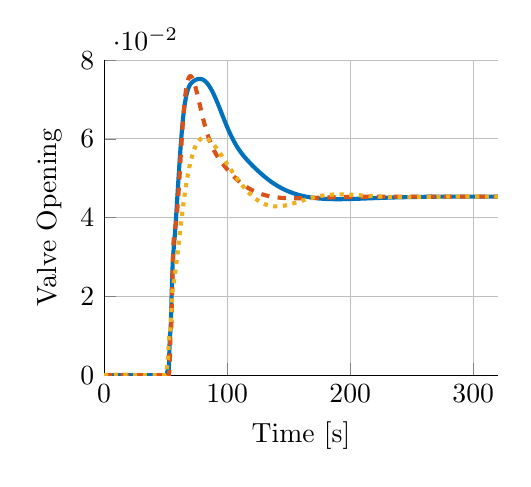
\begin{tikzpicture}

\begin{axis}[%
width=5cm,
height=4cm,
at={(0\linewidth,0\linewidth)},
scale only axis,
xmin=0,
xmax=320,
xlabel={Time [s]},
xmajorgrids,
ymin=0,
ymax=0.08,
ylabel={Valve Opening},
ymajorgrids,
axis background/.style={fill=white},
% title style={font=\bfseries},
% title={Normalized Recycle Valve Opening},
axis x line*=bottom,
axis y line*=left
]
\addplot [color=mycolor1,solid,line width=1.5pt,forget plot]
  table[row sep=crcr]{%
0	1.30651e-06\\
0.25	6.92017e-06\\
0.5	1.05998e-05\\
0.75	1.30927e-05\\
1	1.46601e-05\\
1.25	1.50442e-05\\
1.5	1.42539e-05\\
1.75	1.24228e-05\\
2	9.51022e-06\\
2.25	5.51542e-06\\
2.5	7.24745e-07\\
2.75	0\\
3	0\\
3.25	0\\
3.5	0\\
3.75	0\\
4	0\\
4.25	0\\
4.5	0\\
4.75	0\\
5	0\\
5.25	0\\
5.5	0\\
5.75	0\\
6	0\\
6.25	0\\
6.5	0\\
6.75	0\\
7	0\\
7.25	0\\
7.5	0\\
7.75	0\\
8	0\\
8.25	0\\
8.5	0\\
8.75	0\\
9	0\\
9.25	0\\
9.5	0\\
9.75	0\\
10	0\\
10.25	0\\
10.5	0\\
10.75	0\\
11	0\\
11.25	0\\
11.5	0\\
11.75	0\\
12	0\\
12.25	0\\
12.5	0\\
12.75	0\\
13	0\\
13.25	0\\
13.5	0\\
13.75	0\\
14	0\\
14.25	0\\
14.5	0\\
14.75	0\\
15	0\\
15.25	0\\
15.5	0\\
15.75	0\\
16	0\\
16.25	0\\
16.5	0\\
16.75	0\\
17	0\\
17.25	0\\
17.5	0\\
17.75	0\\
18	0\\
18.25	0\\
18.5	0\\
18.75	0\\
19	0\\
19.25	0\\
19.5	0\\
19.75	0\\
20	0\\
20.25	0\\
20.5	0\\
20.75	0\\
21	0\\
21.25	0\\
21.5	0\\
21.75	0\\
22	0\\
22.25	0\\
22.5	0\\
22.75	0\\
23	0\\
23.25	0\\
23.5	0\\
23.75	0\\
24	0\\
24.25	0\\
24.5	0\\
24.75	0\\
25	0\\
25.25	0\\
25.5	0\\
25.75	0\\
26	0\\
26.25	0\\
26.5	0\\
26.75	0\\
27	0\\
27.25	0\\
27.5	0\\
27.75	0\\
28	0\\
28.25	0\\
28.5	0\\
28.75	0\\
29	0\\
29.25	0\\
29.5	0\\
29.75	0\\
30	0\\
30.25	0\\
30.5	0\\
30.75	0\\
31	0\\
31.25	0\\
31.5	0\\
31.75	0\\
32	0\\
32.25	0\\
32.5	0\\
32.75	0\\
33	0\\
33.25	0\\
33.5	0\\
33.75	0\\
34	0\\
34.25	0\\
34.5	0\\
34.75	0\\
35	0\\
35.25	0\\
35.5	0\\
35.75	0\\
36	0\\
36.25	0\\
36.5	0\\
36.75	0\\
37	0\\
37.25	0\\
37.5	0\\
37.75	0\\
38	0\\
38.25	0\\
38.5	0\\
38.75	0\\
39	0\\
39.25	0\\
39.5	0\\
39.75	0\\
40	0\\
40.25	0\\
40.5	0\\
40.75	0\\
41	0\\
41.25	0\\
41.5	0\\
41.75	0\\
42	0\\
42.25	0\\
42.5	0\\
42.75	0\\
43	0\\
43.25	0\\
43.5	0\\
43.75	0\\
44	0\\
44.25	0\\
44.5	0\\
44.75	0\\
45	0\\
45.25	0\\
45.5	0\\
45.75	0\\
46	0\\
46.25	0\\
46.5	0\\
46.75	0\\
47	0\\
47.25	0\\
47.5	0\\
47.75	0\\
48	0\\
48.25	0\\
48.5	0\\
48.75	0\\
49	0\\
49.25	0\\
49.5	0\\
49.75	0\\
50	0\\
50.25	0\\
50.5	0\\
50.75	0.00010029\\
51	0.000407362\\
51.25	0\\
51.5	0\\
51.75	5.40805e-05\\
52	0.000176293\\
52.25	0.000363014\\
52.5	0.000992407\\
52.75	0.00287787\\
53	0.00554674\\
53.25	0.00839406\\
53.5	0.0100218\\
53.75	0.0106393\\
54	0.0114346\\
54.25	0.0131622\\
54.5	0.0156487\\
54.75	0.0188936\\
55	0.0216522\\
55.25	0.0237894\\
55.5	0.0262732\\
55.75	0.0284355\\
56	0.0298673\\
56.25	0.0309326\\
56.5	0.0319204\\
56.75	0.0328628\\
57	0.0337897\\
57.25	0.0347444\\
57.5	0.0357447\\
57.75	0.0367904\\
58	0.0378773\\
58.25	0.039007\\
58.5	0.0401793\\
58.75	0.0413865\\
59	0.0426192\\
59.25	0.0438703\\
59.5	0.0451331\\
59.75	0.0464002\\
60	0.0476651\\
60.25	0.0489224\\
60.5	0.0501673\\
60.75	0.0513955\\
61	0.0526033\\
61.25	0.0537878\\
61.5	0.0549464\\
61.75	0.056077\\
62	0.057178\\
62.25	0.0582477\\
62.5	0.0592848\\
62.75	0.0602878\\
63	0.0612554\\
63.25	0.062186\\
63.5	0.0630781\\
63.75	0.0639301\\
64	0.0647406\\
64.25	0.0655084\\
64.5	0.0662327\\
64.75	0.0669131\\
65	0.0675499\\
65.25	0.0681441\\
65.5	0.068697\\
65.75	0.0692103\\
66	0.0696861\\
66.25	0.0701266\\
66.5	0.0705345\\
66.75	0.0709129\\
67	0.0712644\\
67.25	0.0715908\\
67.5	0.0718933\\
67.75	0.072173\\
68	0.0724304\\
68.25	0.0726666\\
68.5	0.0728827\\
68.75	0.0730798\\
69	0.0732594\\
69.25	0.0734229\\
69.5	0.0735716\\
69.75	0.0737071\\
70	0.0738307\\
70.25	0.0739435\\
70.5	0.0740469\\
70.75	0.0741418\\
71	0.0742292\\
71.25	0.0743099\\
71.5	0.0743849\\
71.75	0.0744546\\
72	0.0745198\\
72.25	0.074581\\
72.5	0.0746385\\
72.75	0.0746927\\
73	0.074744\\
73.25	0.0747925\\
73.5	0.0748385\\
73.75	0.0748821\\
74	0.0749233\\
74.25	0.0749623\\
74.5	0.074999\\
74.75	0.0750334\\
75	0.0750655\\
75.25	0.0750953\\
75.5	0.0751227\\
75.75	0.0751476\\
76	0.0751699\\
76.25	0.0751895\\
76.5	0.0752063\\
76.75	0.0752202\\
77	0.0752311\\
77.25	0.075239\\
77.5	0.0752436\\
77.75	0.0752449\\
78	0.0752428\\
78.25	0.0752373\\
78.5	0.0752282\\
78.75	0.0752155\\
79	0.0751991\\
79.25	0.0751789\\
79.5	0.0751549\\
79.75	0.0751271\\
80	0.0750954\\
80.25	0.0750597\\
80.5	0.0750201\\
80.75	0.0749765\\
81	0.0749289\\
81.25	0.0748773\\
81.5	0.0748216\\
81.75	0.074762\\
82	0.0746984\\
82.25	0.0746307\\
82.5	0.074559\\
82.75	0.0744834\\
83	0.0744038\\
83.25	0.0743202\\
83.5	0.0742327\\
83.75	0.0741414\\
84	0.0740461\\
84.25	0.0739471\\
84.5	0.0738442\\
84.75	0.0737376\\
85	0.0736273\\
85.25	0.0735133\\
85.5	0.0733957\\
85.75	0.0732745\\
86	0.0731498\\
86.25	0.0730216\\
86.5	0.07289\\
86.75	0.0727551\\
87	0.0726168\\
87.25	0.0724754\\
87.5	0.0723307\\
87.75	0.072183\\
88	0.0720322\\
88.25	0.0718785\\
88.5	0.0717219\\
88.75	0.0715626\\
89	0.0714005\\
89.25	0.0712357\\
89.5	0.0710685\\
89.75	0.0708987\\
90	0.0707266\\
90.25	0.0705522\\
90.5	0.0703756\\
90.75	0.070197\\
91	0.0700163\\
91.25	0.0698337\\
91.5	0.0696494\\
91.75	0.0694633\\
92	0.0692757\\
92.25	0.0690865\\
92.5	0.068896\\
92.75	0.0687042\\
93	0.0685112\\
93.25	0.0683171\\
93.5	0.0681221\\
93.75	0.0679262\\
94	0.0677296\\
94.25	0.0675323\\
94.5	0.0673345\\
94.75	0.0671363\\
95	0.0669377\\
95.25	0.0667389\\
95.5	0.06654\\
95.75	0.0663411\\
96	0.0661422\\
96.25	0.0659436\\
96.5	0.0657452\\
96.75	0.0655472\\
97	0.0653496\\
97.25	0.0651526\\
97.5	0.0649563\\
97.75	0.0647607\\
98	0.064566\\
98.25	0.0643721\\
98.5	0.0641793\\
98.75	0.0639875\\
99	0.0637968\\
99.25	0.0636074\\
99.5	0.0634192\\
99.75	0.0632324\\
100	0.063047\\
100.25	0.062863\\
100.5	0.0626806\\
100.75	0.0624997\\
101	0.0623205\\
101.25	0.0621429\\
101.5	0.0619671\\
101.75	0.061793\\
102	0.0616207\\
102.25	0.0614502\\
102.5	0.0612815\\
102.75	0.0611147\\
103	0.0609499\\
103.25	0.0607869\\
103.5	0.0606259\\
103.75	0.0604668\\
104	0.0603097\\
104.25	0.0601545\\
104.5	0.0600014\\
104.75	0.0598501\\
105	0.0597009\\
105.25	0.0595536\\
105.5	0.0594083\\
105.75	0.0592649\\
106	0.0591235\\
106.25	0.058984\\
106.5	0.0588464\\
106.75	0.0587107\\
107	0.0585769\\
107.25	0.0584449\\
107.5	0.0583148\\
107.75	0.0581864\\
108	0.0580598\\
108.25	0.057935\\
108.5	0.0578119\\
108.75	0.0576905\\
109	0.0575708\\
109.25	0.0574526\\
109.5	0.0573361\\
109.75	0.0572211\\
110	0.0571077\\
110.25	0.0569957\\
110.5	0.0568852\\
110.75	0.0567761\\
111	0.0566683\\
111.25	0.056562\\
111.5	0.0564569\\
111.75	0.0563531\\
112	0.0562505\\
112.25	0.0561491\\
112.5	0.0560489\\
112.75	0.0559498\\
113	0.0558518\\
113.25	0.0557548\\
113.5	0.0556589\\
113.75	0.0555639\\
114	0.0554699\\
114.25	0.0553768\\
114.5	0.0552846\\
114.75	0.0551933\\
115	0.0551027\\
115.25	0.055013\\
115.5	0.054924\\
115.75	0.0548358\\
116	0.0547483\\
116.25	0.0546614\\
116.5	0.0545752\\
116.75	0.0544896\\
117	0.0544047\\
117.25	0.0543203\\
117.5	0.0542365\\
117.75	0.0541532\\
118	0.0540704\\
118.25	0.0539882\\
118.5	0.0539064\\
118.75	0.0538251\\
119	0.0537443\\
119.25	0.0536639\\
119.5	0.0535839\\
119.75	0.0535043\\
120	0.0534252\\
120.25	0.0533464\\
120.5	0.053268\\
120.75	0.0531899\\
121	0.0531123\\
121.25	0.0530349\\
121.5	0.0529579\\
121.75	0.0528813\\
122	0.052805\\
122.25	0.052729\\
122.5	0.0526533\\
122.75	0.0525779\\
123	0.0525029\\
123.25	0.0524282\\
123.5	0.0523537\\
123.75	0.0522796\\
124	0.0522058\\
124.25	0.0521324\\
124.5	0.0520592\\
124.75	0.0519863\\
125	0.0519137\\
125.25	0.0518415\\
125.5	0.0517696\\
125.75	0.0516979\\
126	0.0516266\\
126.25	0.0515557\\
126.5	0.051485\\
126.75	0.0514147\\
127	0.0513447\\
127.25	0.051275\\
127.5	0.0512057\\
127.75	0.0511367\\
128	0.0510681\\
128.25	0.0509998\\
128.5	0.0509318\\
128.75	0.0508642\\
129	0.050797\\
129.25	0.0507302\\
129.5	0.0506637\\
129.75	0.0505976\\
130	0.0505318\\
130.25	0.0504665\\
130.5	0.0504015\\
130.75	0.050337\\
131	0.0502728\\
131.25	0.050209\\
131.5	0.0501456\\
131.75	0.0500827\\
132	0.0500201\\
132.25	0.049958\\
132.5	0.0498962\\
132.75	0.0498349\\
133	0.049774\\
133.25	0.0497136\\
133.5	0.0496535\\
133.75	0.0495939\\
134	0.0495348\\
134.25	0.049476\\
134.5	0.0494178\\
134.75	0.0493599\\
135	0.0493025\\
135.25	0.0492455\\
135.5	0.049189\\
135.75	0.0491329\\
136	0.0490773\\
136.25	0.0490221\\
136.5	0.0489674\\
136.75	0.0489131\\
137	0.0488593\\
137.25	0.0488059\\
137.5	0.048753\\
137.75	0.0487006\\
138	0.0486485\\
138.25	0.048597\\
138.5	0.0485459\\
138.75	0.0484952\\
139	0.048445\\
139.25	0.0483952\\
139.5	0.0483459\\
139.75	0.048297\\
140	0.0482486\\
140.25	0.0482007\\
140.5	0.0481531\\
140.75	0.048106\\
141	0.0480594\\
141.25	0.0480132\\
141.5	0.0479674\\
141.75	0.0479221\\
142	0.0478772\\
142.25	0.0478327\\
142.5	0.0477887\\
142.75	0.0477451\\
143	0.0477019\\
143.25	0.0476592\\
143.5	0.0476168\\
143.75	0.0475749\\
144	0.0475334\\
144.25	0.0474924\\
144.5	0.0474517\\
144.75	0.0474114\\
145	0.0473716\\
145.25	0.0473322\\
145.5	0.0472931\\
145.75	0.0472545\\
146	0.0472162\\
146.25	0.0471784\\
146.5	0.047141\\
146.75	0.0471039\\
147	0.0470672\\
147.25	0.0470309\\
147.5	0.046995\\
147.75	0.0469595\\
148	0.0469244\\
148.25	0.0468896\\
148.5	0.0468552\\
148.75	0.0468212\\
149	0.0467875\\
149.25	0.0467542\\
149.5	0.0467213\\
149.75	0.0466887\\
150	0.0466565\\
150.25	0.0466246\\
150.5	0.0465931\\
150.75	0.046562\\
151	0.0465312\\
151.25	0.0465007\\
151.5	0.0464706\\
151.75	0.0464408\\
152	0.0464113\\
152.25	0.0463822\\
152.5	0.0463534\\
152.75	0.046325\\
153	0.0462969\\
153.25	0.0462691\\
153.5	0.0462416\\
153.75	0.0462144\\
154	0.0461876\\
154.25	0.0461611\\
154.5	0.0461349\\
154.75	0.046109\\
155	0.0460834\\
155.25	0.0460581\\
155.5	0.0460332\\
155.75	0.0460085\\
156	0.0459842\\
156.25	0.0459601\\
156.5	0.0459363\\
156.75	0.0459129\\
157	0.0458897\\
157.25	0.0458668\\
157.5	0.0458442\\
157.75	0.0458219\\
158	0.0457999\\
158.25	0.0457782\\
158.5	0.0457567\\
158.75	0.0457356\\
159	0.0457147\\
159.25	0.0456941\\
159.5	0.0456737\\
159.75	0.0456536\\
160	0.0456338\\
160.25	0.0456143\\
160.5	0.045595\\
160.75	0.045576\\
161	0.0455573\\
161.25	0.0455388\\
161.5	0.0455206\\
161.75	0.0455026\\
162	0.0454849\\
162.25	0.0454675\\
162.5	0.0454503\\
162.75	0.0454333\\
163	0.0454166\\
163.25	0.0454001\\
163.5	0.0453839\\
163.75	0.0453679\\
164	0.0453522\\
164.25	0.0453367\\
164.5	0.0453215\\
164.75	0.0453064\\
165	0.0452917\\
165.25	0.0452771\\
165.5	0.0452628\\
165.75	0.0452487\\
166	0.0452348\\
166.25	0.0452211\\
166.5	0.0452077\\
166.75	0.0451945\\
167	0.0451815\\
167.25	0.0451687\\
167.5	0.0451562\\
167.75	0.0451438\\
168	0.0451317\\
168.25	0.0451198\\
168.5	0.0451081\\
168.75	0.0450966\\
169	0.0450853\\
169.25	0.0450742\\
169.5	0.0450633\\
169.75	0.0450526\\
170	0.0450421\\
170.25	0.0450318\\
170.5	0.0450216\\
170.75	0.0450117\\
171	0.045002\\
171.25	0.0449924\\
171.5	0.0449831\\
171.75	0.0449739\\
172	0.0449649\\
172.25	0.0449561\\
172.5	0.0449475\\
172.75	0.044939\\
173	0.0449308\\
173.25	0.0449227\\
173.5	0.0449147\\
173.75	0.044907\\
174	0.0448994\\
174.25	0.044892\\
174.5	0.0448847\\
174.75	0.0448776\\
175	0.0448707\\
175.25	0.0448639\\
175.5	0.0448573\\
175.75	0.0448509\\
176	0.0448446\\
176.25	0.0448384\\
176.5	0.0448325\\
176.75	0.0448266\\
177	0.0448209\\
177.25	0.0448154\\
177.5	0.04481\\
177.75	0.0448047\\
178	0.0447996\\
178.25	0.0447947\\
178.5	0.0447898\\
178.75	0.0447851\\
179	0.0447806\\
179.25	0.0447762\\
179.5	0.0447719\\
179.75	0.0447677\\
180	0.0447637\\
180.25	0.0447598\\
180.5	0.044756\\
180.75	0.0447524\\
181	0.0447488\\
181.25	0.0447454\\
181.5	0.0447422\\
181.75	0.044739\\
182	0.044736\\
182.25	0.044733\\
182.5	0.0447302\\
182.75	0.0447275\\
183	0.0447249\\
183.25	0.0447224\\
183.5	0.0447201\\
183.75	0.0447178\\
184	0.0447156\\
184.25	0.0447136\\
184.5	0.0447116\\
184.75	0.0447098\\
185	0.044708\\
185.25	0.0447064\\
185.5	0.0447048\\
185.75	0.0447034\\
186	0.044702\\
186.25	0.0447008\\
186.5	0.0446996\\
186.75	0.0446985\\
187	0.0446975\\
187.25	0.0446966\\
187.5	0.0446958\\
187.75	0.044695\\
188	0.0446944\\
188.25	0.0446938\\
188.5	0.0446934\\
188.75	0.044693\\
189	0.0446926\\
189.25	0.0446924\\
189.5	0.0446922\\
189.75	0.0446921\\
190	0.0446921\\
190.25	0.0446922\\
190.5	0.0446923\\
190.75	0.0446925\\
191	0.0446928\\
191.25	0.0446931\\
191.5	0.0446935\\
191.75	0.044694\\
192	0.0446945\\
192.25	0.0446952\\
192.5	0.0446958\\
192.75	0.0446966\\
193	0.0446973\\
193.25	0.0446982\\
193.5	0.0446991\\
193.75	0.0447001\\
194	0.0447011\\
194.25	0.0447022\\
194.5	0.0447033\\
194.75	0.0447045\\
195	0.0447058\\
195.25	0.0447071\\
195.5	0.0447084\\
195.75	0.0447098\\
196	0.0447113\\
196.25	0.0447128\\
196.5	0.0447143\\
196.75	0.0447159\\
197	0.0447176\\
197.25	0.0447193\\
197.5	0.044721\\
197.75	0.0447228\\
198	0.0447246\\
198.25	0.0447264\\
198.5	0.0447283\\
198.75	0.0447303\\
199	0.0447322\\
199.25	0.0447343\\
199.5	0.0447363\\
199.75	0.0447384\\
200	0.0447405\\
200.25	0.0447427\\
200.5	0.0447448\\
200.75	0.0447471\\
201	0.0447493\\
201.25	0.0447516\\
201.5	0.0447539\\
201.75	0.0447563\\
202	0.0447586\\
202.25	0.0447611\\
202.5	0.0447635\\
202.75	0.0447659\\
203	0.0447684\\
203.25	0.0447709\\
203.5	0.0447735\\
203.75	0.044776\\
204	0.0447786\\
204.25	0.0447812\\
204.5	0.0447838\\
204.75	0.0447865\\
205	0.0447892\\
205.25	0.0447919\\
205.5	0.0447946\\
205.75	0.0447973\\
206	0.0448\\
206.25	0.0448028\\
206.5	0.0448056\\
206.75	0.0448084\\
207	0.0448112\\
207.25	0.044814\\
207.5	0.0448169\\
207.75	0.0448197\\
208	0.0448226\\
208.25	0.0448255\\
208.5	0.0448284\\
208.75	0.0448313\\
209	0.0448342\\
209.25	0.0448372\\
209.5	0.0448401\\
209.75	0.0448431\\
210	0.044846\\
210.25	0.044849\\
210.5	0.044852\\
210.75	0.044855\\
211	0.044858\\
211.25	0.044861\\
211.5	0.044864\\
211.75	0.044867\\
212	0.04487\\
212.25	0.044873\\
212.5	0.0448761\\
212.75	0.0448791\\
213	0.0448821\\
213.25	0.0448852\\
213.5	0.0448882\\
213.75	0.0448913\\
214	0.0448943\\
214.25	0.0448974\\
214.5	0.0449004\\
214.75	0.0449035\\
215	0.0449066\\
215.25	0.0449096\\
215.5	0.0449127\\
215.75	0.0449157\\
216	0.0449188\\
216.25	0.0449218\\
216.5	0.0449249\\
216.75	0.044928\\
217	0.044931\\
217.25	0.0449341\\
217.5	0.0449371\\
217.75	0.0449401\\
218	0.0449432\\
218.25	0.0449462\\
218.5	0.0449493\\
218.75	0.0449523\\
219	0.0449553\\
219.25	0.0449583\\
219.5	0.0449613\\
219.75	0.0449644\\
220	0.0449674\\
220.25	0.0449704\\
220.5	0.0449733\\
220.75	0.0449763\\
221	0.0449793\\
221.25	0.0449823\\
221.5	0.0449853\\
221.75	0.0449882\\
222	0.0449912\\
222.25	0.0449941\\
222.5	0.044997\\
222.75	0.045\\
223	0.0450029\\
223.25	0.0450058\\
223.5	0.0450087\\
223.75	0.0450116\\
224	0.0450145\\
224.25	0.0450174\\
224.5	0.0450202\\
224.75	0.0450231\\
225	0.0450259\\
225.25	0.0450288\\
225.5	0.0450316\\
225.75	0.0450344\\
226	0.0450372\\
226.25	0.04504\\
226.5	0.0450428\\
226.75	0.0450456\\
227	0.0450483\\
227.25	0.0450511\\
227.5	0.0450538\\
227.75	0.0450565\\
228	0.0450593\\
228.25	0.045062\\
228.5	0.0450646\\
228.75	0.0450673\\
229	0.04507\\
229.25	0.0450727\\
229.5	0.0450753\\
229.75	0.0450779\\
230	0.0450805\\
230.25	0.0450832\\
230.5	0.0450857\\
230.75	0.0450883\\
231	0.0450909\\
231.25	0.0450934\\
231.5	0.045096\\
231.75	0.0450985\\
232	0.045101\\
232.25	0.0451035\\
232.5	0.045106\\
232.75	0.0451085\\
233	0.045111\\
233.25	0.0451134\\
233.5	0.0451158\\
233.75	0.0451183\\
234	0.0451207\\
234.25	0.0451231\\
234.5	0.0451254\\
234.75	0.0451278\\
235	0.0451302\\
235.25	0.0451325\\
235.5	0.0451348\\
235.75	0.0451371\\
236	0.0451394\\
236.25	0.0451417\\
236.5	0.045144\\
236.75	0.0451462\\
237	0.0451485\\
237.25	0.0451507\\
237.5	0.0451529\\
237.75	0.0451551\\
238	0.0451573\\
238.25	0.0451594\\
238.5	0.0451616\\
238.75	0.0451637\\
239	0.0451658\\
239.25	0.0451679\\
239.5	0.04517\\
239.75	0.0451721\\
240	0.0451742\\
240.25	0.0451762\\
240.5	0.0451783\\
240.75	0.0451803\\
241	0.0451823\\
241.25	0.0451843\\
241.5	0.0451863\\
241.75	0.0451882\\
242	0.0451902\\
242.25	0.0451921\\
242.5	0.045194\\
242.75	0.0451959\\
243	0.0451978\\
243.25	0.0451997\\
243.5	0.0452016\\
243.75	0.0452034\\
244	0.0452053\\
244.25	0.0452071\\
244.5	0.0452089\\
244.75	0.0452107\\
245	0.0452124\\
245.25	0.0452142\\
245.5	0.045216\\
245.75	0.0452177\\
246	0.0452194\\
246.25	0.0452211\\
246.5	0.0452228\\
246.75	0.0452245\\
247	0.0452262\\
247.25	0.0452278\\
247.5	0.0452294\\
247.75	0.0452311\\
248	0.0452327\\
248.25	0.0452343\\
248.5	0.0452358\\
248.75	0.0452374\\
249	0.045239\\
249.25	0.0452405\\
249.5	0.045242\\
249.75	0.0452435\\
250	0.045245\\
250.25	0.0452465\\
250.5	0.045248\\
250.75	0.0452495\\
251	0.0452509\\
251.25	0.0452523\\
251.5	0.0452537\\
251.75	0.0452552\\
252	0.0452565\\
252.25	0.0452579\\
252.5	0.0452593\\
252.75	0.0452606\\
253	0.045262\\
253.25	0.0452633\\
253.5	0.0452646\\
253.75	0.0452659\\
254	0.0452672\\
254.25	0.0452685\\
254.5	0.0452698\\
254.75	0.045271\\
255	0.0452723\\
255.25	0.0452735\\
255.5	0.0452747\\
255.75	0.0452759\\
256	0.0452771\\
256.25	0.0452783\\
256.5	0.0452794\\
256.75	0.0452806\\
257	0.0452817\\
257.25	0.0452829\\
257.5	0.045284\\
257.75	0.0452851\\
258	0.0452862\\
258.25	0.0452873\\
258.5	0.0452883\\
258.75	0.0452894\\
259	0.0452904\\
259.25	0.0452915\\
259.5	0.0452925\\
259.75	0.0452935\\
260	0.0452945\\
260.25	0.0452955\\
260.5	0.0452965\\
260.75	0.0452975\\
261	0.0452984\\
261.25	0.0452994\\
261.5	0.0453003\\
261.75	0.0453012\\
262	0.0453022\\
262.25	0.0453031\\
262.5	0.045304\\
262.75	0.0453049\\
263	0.0453057\\
263.25	0.0453066\\
263.5	0.0453074\\
263.75	0.0453083\\
264	0.0453091\\
264.25	0.0453099\\
264.5	0.0453108\\
264.75	0.0453116\\
265	0.0453124\\
265.25	0.0453131\\
265.5	0.0453139\\
265.75	0.0453147\\
266	0.0453154\\
266.25	0.0453162\\
266.5	0.0453169\\
266.75	0.0453177\\
267	0.0453184\\
267.25	0.0453191\\
267.5	0.0453198\\
267.75	0.0453205\\
268	0.0453212\\
268.25	0.0453218\\
268.5	0.0453225\\
268.75	0.0453232\\
269	0.0453238\\
269.25	0.0453244\\
269.5	0.0453251\\
269.75	0.0453257\\
270	0.0453263\\
270.25	0.0453269\\
270.5	0.0453275\\
270.75	0.0453281\\
271	0.0453287\\
271.25	0.0453292\\
271.5	0.0453298\\
271.75	0.0453304\\
272	0.0453309\\
272.25	0.0453314\\
272.5	0.045332\\
272.75	0.0453325\\
273	0.045333\\
273.25	0.0453335\\
273.5	0.045334\\
273.75	0.0453345\\
274	0.045335\\
274.25	0.0453355\\
274.5	0.045336\\
274.75	0.0453364\\
275	0.0453369\\
275.25	0.0453373\\
275.5	0.0453378\\
275.75	0.0453382\\
276	0.0453386\\
276.25	0.0453391\\
276.5	0.0453395\\
276.75	0.0453399\\
277	0.0453403\\
277.25	0.0453407\\
277.5	0.0453411\\
277.75	0.0453415\\
278	0.0453418\\
278.25	0.0453422\\
278.5	0.0453426\\
278.75	0.0453429\\
279	0.0453433\\
279.25	0.0453436\\
279.5	0.045344\\
279.75	0.0453443\\
280	0.0453446\\
280.25	0.045345\\
280.5	0.0453453\\
280.75	0.0453456\\
281	0.0453459\\
281.25	0.0453462\\
281.5	0.0453465\\
281.75	0.0453468\\
282	0.0453471\\
282.25	0.0453473\\
282.5	0.0453476\\
282.75	0.0453479\\
283	0.0453481\\
283.25	0.0453484\\
283.5	0.0453486\\
283.75	0.0453489\\
284	0.0453491\\
284.25	0.0453494\\
284.5	0.0453496\\
284.75	0.0453498\\
285	0.0453501\\
285.25	0.0453503\\
285.5	0.0453505\\
285.75	0.0453507\\
286	0.0453509\\
286.25	0.0453511\\
286.5	0.0453513\\
286.75	0.0453515\\
287	0.0453517\\
287.25	0.0453518\\
287.5	0.045352\\
287.75	0.0453522\\
288	0.0453524\\
288.25	0.0453525\\
288.5	0.0453527\\
288.75	0.0453529\\
289	0.045353\\
289.25	0.0453532\\
289.5	0.0453533\\
289.75	0.0453534\\
290	0.0453536\\
290.25	0.0453537\\
290.5	0.0453538\\
290.75	0.045354\\
291	0.0453541\\
291.25	0.0453542\\
291.5	0.0453543\\
291.75	0.0453544\\
292	0.0453545\\
292.25	0.0453546\\
292.5	0.0453547\\
292.75	0.0453548\\
293	0.0453549\\
293.25	0.045355\\
293.5	0.0453551\\
293.75	0.0453552\\
294	0.0453553\\
294.25	0.0453554\\
294.5	0.0453554\\
294.75	0.0453555\\
295	0.0453556\\
295.25	0.0453557\\
295.5	0.0453557\\
295.75	0.0453558\\
296	0.0453558\\
296.25	0.0453559\\
296.5	0.045356\\
296.75	0.045356\\
297	0.0453561\\
297.25	0.0453561\\
297.5	0.0453561\\
297.75	0.0453562\\
298	0.0453562\\
298.25	0.0453563\\
298.5	0.0453563\\
298.75	0.0453563\\
299	0.0453564\\
299.25	0.0453564\\
299.5	0.0453564\\
299.75	0.0453564\\
300	0.0453565\\
300.25	0.0453565\\
300.5	0.0453565\\
300.75	0.0453565\\
301	0.0453565\\
301.25	0.0453565\\
301.5	0.0453565\\
301.75	0.0453565\\
302	0.0453565\\
302.25	0.0453565\\
302.5	0.0453565\\
302.75	0.0453565\\
303	0.0453565\\
303.25	0.0453565\\
303.5	0.0453565\\
303.75	0.0453565\\
304	0.0453565\\
304.25	0.0453565\\
304.5	0.0453565\\
304.75	0.0453565\\
305	0.0453564\\
305.25	0.0453564\\
305.5	0.0453564\\
305.75	0.0453564\\
306	0.0453564\\
306.25	0.0453563\\
306.5	0.0453563\\
306.75	0.0453563\\
307	0.0453563\\
307.25	0.0453562\\
307.5	0.0453562\\
307.75	0.0453562\\
308	0.0453561\\
308.25	0.0453561\\
308.5	0.0453561\\
308.75	0.045356\\
309	0.045356\\
309.25	0.0453559\\
309.5	0.0453559\\
309.75	0.0453559\\
310	0.0453558\\
310.25	0.0453558\\
310.5	0.0453557\\
310.75	0.0453557\\
311	0.0453556\\
311.25	0.0453556\\
311.5	0.0453555\\
311.75	0.0453555\\
312	0.0453554\\
312.25	0.0453554\\
312.5	0.0453553\\
312.75	0.0453553\\
313	0.0453552\\
313.25	0.0453552\\
313.5	0.0453551\\
313.75	0.0453551\\
314	0.045355\\
314.25	0.0453549\\
314.5	0.0453549\\
314.75	0.0453548\\
315	0.0453548\\
315.25	0.0453547\\
315.5	0.0453546\\
315.75	0.0453546\\
316	0.0453545\\
316.25	0.0453545\\
316.5	0.0453544\\
316.75	0.0453543\\
317	0.0453543\\
317.25	0.0453542\\
317.5	0.0453541\\
317.75	0.0453541\\
318	0.045354\\
318.25	0.0453539\\
318.5	0.0453539\\
318.75	0.0453538\\
319	0.0453537\\
319.25	0.0453537\\
319.5	0.0453536\\
319.75	0.0453535\\
320	0.0453535\\
320.25	0.0453534\\
320.5	0.0453533\\
320.75	0.0453532\\
321	0.0453532\\
321.25	0.0453531\\
321.5	0.045353\\
321.75	0.045353\\
322	0.0453529\\
322.25	0.0453528\\
322.5	0.0453527\\
322.75	0.0453527\\
323	0.0453526\\
323.25	0.0453525\\
323.5	0.0453525\\
323.75	0.0453524\\
324	0.0453523\\
324.25	0.0453522\\
324.5	0.0453522\\
324.75	0.0453521\\
325	0.045352\\
325.25	0.0453519\\
325.5	0.0453519\\
325.75	0.0453518\\
326	0.0453517\\
326.25	0.0453516\\
326.5	0.0453516\\
326.75	0.0453515\\
327	0.0453514\\
327.25	0.0453513\\
327.5	0.0453513\\
327.75	0.0453512\\
328	0.0453511\\
328.25	0.045351\\
328.5	0.045351\\
328.75	0.0453509\\
329	0.0453508\\
329.25	0.0453507\\
329.5	0.0453507\\
329.75	0.0453506\\
330	0.0453505\\
330.25	0.0453505\\
330.5	0.0453504\\
330.75	0.0453503\\
331	0.0453502\\
331.25	0.0453502\\
331.5	0.0453501\\
331.75	0.04535\\
332	0.0453499\\
332.25	0.0453499\\
332.5	0.0453498\\
332.75	0.0453497\\
333	0.0453496\\
333.25	0.0453496\\
333.5	0.0453495\\
333.75	0.0453494\\
334	0.0453494\\
334.25	0.0453493\\
334.5	0.0453492\\
334.75	0.0453491\\
335	0.0453491\\
335.25	0.045349\\
335.5	0.0453489\\
335.75	0.0453489\\
336	0.0453488\\
336.25	0.0453487\\
336.5	0.0453486\\
336.75	0.0453486\\
337	0.0453485\\
337.25	0.0453484\\
337.5	0.0453484\\
337.75	0.0453483\\
338	0.0453482\\
338.25	0.0453482\\
338.5	0.0453481\\
338.75	0.045348\\
339	0.045348\\
339.25	0.0453479\\
339.5	0.0453478\\
339.75	0.0453478\\
340	0.0453477\\
340.25	0.0453476\\
340.5	0.0453476\\
340.75	0.0453475\\
341	0.0453474\\
341.25	0.0453474\\
341.5	0.0453473\\
341.75	0.0453472\\
342	0.0453472\\
342.25	0.0453471\\
342.5	0.045347\\
342.75	0.045347\\
343	0.0453469\\
343.25	0.0453469\\
343.5	0.0453468\\
343.75	0.0453467\\
344	0.0453467\\
344.25	0.0453466\\
344.5	0.0453466\\
344.75	0.0453465\\
345	0.0453464\\
345.25	0.0453464\\
345.5	0.0453463\\
345.75	0.0453463\\
346	0.0453462\\
346.25	0.0453461\\
346.5	0.0453461\\
346.75	0.045346\\
347	0.045346\\
347.25	0.0453459\\
347.5	0.0453459\\
347.75	0.0453458\\
348	0.0453457\\
348.25	0.0453457\\
348.5	0.0453456\\
348.75	0.0453456\\
349	0.0453455\\
349.25	0.0453455\\
349.5	0.0453454\\
349.75	0.0453454\\
350	0.0453453\\
350.25	0.0453452\\
350.5	0.0453452\\
350.75	0.0453451\\
351	0.0453451\\
351.25	0.045345\\
351.5	0.045345\\
351.75	0.0453449\\
352	0.0453449\\
352.25	0.0453448\\
352.5	0.0453448\\
352.75	0.0453447\\
353	0.0453447\\
353.25	0.0453446\\
353.5	0.0453446\\
353.75	0.0453445\\
354	0.0453445\\
354.25	0.0453444\\
354.5	0.0453444\\
354.75	0.0453444\\
355	0.0453443\\
355.25	0.0453443\\
355.5	0.0453442\\
355.75	0.0453442\\
356	0.0453441\\
356.25	0.0453441\\
356.5	0.045344\\
356.75	0.045344\\
357	0.045344\\
357.25	0.0453439\\
357.5	0.0453439\\
357.75	0.0453438\\
358	0.0453438\\
358.25	0.0453437\\
358.5	0.0453437\\
358.75	0.0453437\\
359	0.0453436\\
359.25	0.0453436\\
359.5	0.0453435\\
359.75	0.0453435\\
360	0.0453435\\
360.25	0.0453434\\
360.5	0.0453434\\
360.75	0.0453433\\
361	0.0453433\\
361.25	0.0453433\\
361.5	0.0453432\\
361.75	0.0453432\\
362	0.0453432\\
362.25	0.0453431\\
362.5	0.0453431\\
362.75	0.045343\\
363	0.045343\\
363.25	0.045343\\
363.5	0.0453429\\
363.75	0.0453429\\
364	0.0453429\\
364.25	0.0453428\\
364.5	0.0453428\\
364.75	0.0453428\\
365	0.0453427\\
365.25	0.0453427\\
365.5	0.0453427\\
365.75	0.0453426\\
366	0.0453426\\
366.25	0.0453426\\
366.5	0.0453425\\
366.75	0.0453425\\
367	0.0453425\\
367.25	0.0453425\\
367.5	0.0453424\\
367.75	0.0453424\\
368	0.0453424\\
368.25	0.0453423\\
368.5	0.0453423\\
368.75	0.0453423\\
369	0.0453423\\
369.25	0.0453422\\
369.5	0.0453422\\
369.75	0.0453422\\
370	0.0453421\\
370.25	0.0453421\\
370.5	0.0453421\\
370.75	0.0453421\\
371	0.045342\\
371.25	0.045342\\
371.5	0.045342\\
371.75	0.045342\\
372	0.0453419\\
372.25	0.0453419\\
372.5	0.0453419\\
372.75	0.0453419\\
373	0.0453418\\
373.25	0.0453418\\
373.5	0.0453418\\
373.75	0.0453418\\
374	0.0453417\\
374.25	0.0453417\\
374.5	0.0453417\\
374.75	0.0453417\\
375	0.0453417\\
375.25	0.0453416\\
375.5	0.0453416\\
375.75	0.0453416\\
376	0.0453416\\
376.25	0.0453416\\
376.5	0.0453415\\
376.75	0.0453415\\
377	0.0453415\\
377.25	0.0453415\\
377.5	0.0453415\\
377.75	0.0453414\\
378	0.0453414\\
378.25	0.0453414\\
378.5	0.0453414\\
378.75	0.0453414\\
379	0.0453413\\
379.25	0.0453413\\
379.5	0.0453413\\
379.75	0.0453413\\
380	0.0453413\\
380.25	0.0453413\\
380.5	0.0453412\\
380.75	0.0453412\\
381	0.0453412\\
381.25	0.0453412\\
381.5	0.0453412\\
381.75	0.0453412\\
382	0.0453412\\
382.25	0.0453411\\
382.5	0.0453411\\
382.75	0.0453411\\
383	0.0453411\\
383.25	0.0453411\\
383.5	0.0453411\\
383.75	0.0453411\\
384	0.045341\\
384.25	0.045341\\
384.5	0.045341\\
384.75	0.045341\\
385	0.045341\\
385.25	0.045341\\
385.5	0.045341\\
385.75	0.045341\\
386	0.0453409\\
386.25	0.0453409\\
386.5	0.0453409\\
386.75	0.0453409\\
387	0.0453409\\
387.25	0.0453409\\
387.5	0.0453409\\
387.75	0.0453409\\
388	0.0453408\\
388.25	0.0453408\\
388.5	0.0453408\\
388.75	0.0453408\\
389	0.0453408\\
389.25	0.0453408\\
389.5	0.0453408\\
389.75	0.0453408\\
390	0.0453408\\
390.25	0.0453408\\
390.5	0.0453408\\
390.75	0.0453407\\
391	0.0453407\\
391.25	0.0453407\\
391.5	0.0453407\\
391.75	0.0453407\\
392	0.0453407\\
392.25	0.0453407\\
392.5	0.0453407\\
392.75	0.0453407\\
393	0.0453407\\
393.25	0.0453407\\
393.5	0.0453407\\
393.75	0.0453406\\
394	0.0453406\\
394.25	0.0453406\\
394.5	0.0453406\\
394.75	0.0453406\\
395	0.0453406\\
395.25	0.0453406\\
395.5	0.0453406\\
395.75	0.0453406\\
396	0.0453406\\
396.25	0.0453406\\
396.5	0.0453406\\
396.75	0.0453406\\
397	0.0453406\\
397.25	0.0453406\\
397.5	0.0453406\\
397.75	0.0453405\\
398	0.0453405\\
398.25	0.0453405\\
398.5	0.0453405\\
398.75	0.0453405\\
399	0.0453405\\
399.25	0.0453405\\
399.5	0.0453405\\
399.75	0.0453405\\
400	0.0453405\\
400.25	0.0453405\\
400.5	0.0453405\\
400.75	0.0453405\\
401	0.0453405\\
401.25	0.0453405\\
401.5	0.0453405\\
401.75	0.0453405\\
402	0.0453405\\
402.25	0.0453405\\
402.5	0.0453405\\
402.75	0.0453405\\
403	0.0453405\\
403.25	0.0453405\\
403.5	0.0453405\\
403.75	0.0453405\\
404	0.0453405\\
404.25	0.0453405\\
404.5	0.0453404\\
404.75	0.0453404\\
405	0.0453404\\
405.25	0.0453404\\
405.5	0.0453404\\
405.75	0.0453404\\
406	0.0453404\\
406.25	0.0453404\\
406.5	0.0453404\\
406.75	0.0453404\\
407	0.0453404\\
407.25	0.0453404\\
407.5	0.0453404\\
407.75	0.0453404\\
408	0.0453404\\
408.25	0.0453404\\
408.5	0.0453404\\
408.75	0.0453404\\
409	0.0453404\\
409.25	0.0453404\\
409.5	0.0453404\\
409.75	0.0453404\\
410	0.0453404\\
410.25	0.0453404\\
410.5	0.0453404\\
410.75	0.0453404\\
411	0.0453404\\
411.25	0.0453404\\
411.5	0.0453404\\
411.75	0.0453404\\
412	0.0453404\\
412.25	0.0453404\\
412.5	0.0453404\\
412.75	0.0453404\\
413	0.0453404\\
413.25	0.0453404\\
413.5	0.0453404\\
413.75	0.0453404\\
414	0.0453404\\
414.25	0.0453404\\
414.5	0.0453404\\
414.75	0.0453404\\
415	0.0453404\\
415.25	0.0453404\\
415.5	0.0453404\\
415.75	0.0453404\\
416	0.0453404\\
416.25	0.0453404\\
416.5	0.0453404\\
416.75	0.0453404\\
417	0.0453404\\
417.25	0.0453404\\
417.5	0.0453404\\
417.75	0.0453404\\
418	0.0453404\\
418.25	0.0453404\\
418.5	0.0453404\\
418.75	0.0453404\\
419	0.0453404\\
419.25	0.0453404\\
419.5	0.0453404\\
419.75	0.0453404\\
420	0.0453404\\
420.25	0.0453404\\
420.5	0.0453404\\
420.75	0.0453404\\
421	0.0453404\\
421.25	0.0453404\\
421.5	0.0453404\\
421.75	0.0453404\\
422	0.0453404\\
422.25	0.0453404\\
422.5	0.0453404\\
422.75	0.0453404\\
423	0.0453404\\
423.25	0.0453404\\
423.5	0.0453404\\
423.75	0.0453404\\
424	0.0453404\\
424.25	0.0453404\\
424.5	0.0453404\\
424.75	0.0453404\\
425	0.0453404\\
425.25	0.0453404\\
425.5	0.0453404\\
425.75	0.0453404\\
426	0.0453404\\
426.25	0.0453404\\
426.5	0.0453404\\
426.75	0.0453404\\
427	0.0453404\\
427.25	0.0453404\\
427.5	0.0453404\\
427.75	0.0453404\\
428	0.0453405\\
428.25	0.0453405\\
428.5	0.0453405\\
428.75	0.0453405\\
429	0.0453405\\
429.25	0.0453405\\
429.5	0.0453405\\
429.75	0.0453405\\
430	0.0453405\\
430.25	0.0453405\\
430.5	0.0453405\\
430.75	0.0453405\\
431	0.0453405\\
431.25	0.0453405\\
431.5	0.0453405\\
431.75	0.0453405\\
432	0.0453405\\
432.25	0.0453405\\
432.5	0.0453405\\
432.75	0.0453405\\
433	0.0453405\\
433.25	0.0453405\\
433.5	0.0453405\\
433.75	0.0453405\\
434	0.0453405\\
434.25	0.0453405\\
434.5	0.0453405\\
434.75	0.0453405\\
435	0.0453405\\
435.25	0.0453405\\
435.5	0.0453405\\
435.75	0.0453405\\
436	0.0453405\\
436.25	0.0453405\\
436.5	0.0453405\\
436.75	0.0453405\\
437	0.0453405\\
437.25	0.0453405\\
437.5	0.0453405\\
437.75	0.0453405\\
438	0.0453405\\
438.25	0.0453405\\
438.5	0.0453405\\
438.75	0.0453405\\
439	0.0453405\\
439.25	0.0453405\\
439.5	0.0453405\\
439.75	0.0453405\\
440	0.0453405\\
440.25	0.0453405\\
440.5	0.0453405\\
440.75	0.0453405\\
441	0.0453405\\
441.25	0.0453405\\
441.5	0.0453405\\
441.75	0.0453405\\
442	0.0453405\\
442.25	0.0453405\\
442.5	0.0453406\\
442.75	0.0453406\\
443	0.0453406\\
443.25	0.0453406\\
443.5	0.0453406\\
443.75	0.0453406\\
444	0.0453406\\
444.25	0.0453406\\
444.5	0.0453406\\
444.75	0.0453406\\
445	0.0453406\\
445.25	0.0453406\\
445.5	0.0453406\\
445.75	0.0453406\\
446	0.0453406\\
446.25	0.0453406\\
446.5	0.0453406\\
446.75	0.0453406\\
447	0.0453406\\
447.25	0.0453406\\
447.5	0.0453406\\
447.75	0.0453406\\
448	0.0453406\\
448.25	0.0453406\\
448.5	0.0453406\\
448.75	0.0453406\\
449	0.0453406\\
449.25	0.0453406\\
449.5	0.0453406\\
449.75	0.0453406\\
450	0.0453406\\
450.25	0.0453406\\
450.5	0.0453406\\
450.75	0.0453406\\
451	0.0453406\\
451.25	0.0453406\\
451.5	0.0453406\\
451.75	0.0453406\\
452	0.0453406\\
452.25	0.0453406\\
452.5	0.0453406\\
452.75	0.0453406\\
453	0.0453406\\
453.25	0.0453406\\
453.5	0.0453406\\
453.75	0.0453406\\
454	0.0453406\\
454.25	0.0453406\\
454.5	0.0453406\\
454.75	0.0453406\\
455	0.0453406\\
455.25	0.0453406\\
455.5	0.0453406\\
455.75	0.0453406\\
456	0.0453406\\
456.25	0.0453406\\
456.5	0.0453406\\
456.75	0.0453406\\
457	0.0453406\\
457.25	0.0453406\\
457.5	0.0453407\\
457.75	0.0453407\\
458	0.0453407\\
458.25	0.0453407\\
458.5	0.0453407\\
458.75	0.0453407\\
459	0.0453407\\
459.25	0.0453407\\
459.5	0.0453407\\
459.75	0.0453407\\
460	0.0453407\\
460.25	0.0453407\\
460.5	0.0453407\\
460.75	0.0453407\\
461	0.0453407\\
461.25	0.0453407\\
461.5	0.0453407\\
461.75	0.0453407\\
462	0.0453407\\
462.25	0.0453407\\
462.5	0.0453407\\
462.75	0.0453407\\
463	0.0453407\\
463.25	0.0453407\\
463.5	0.0453407\\
463.75	0.0453407\\
464	0.0453407\\
464.25	0.0453407\\
464.5	0.0453407\\
464.75	0.0453407\\
465	0.0453407\\
465.25	0.0453407\\
465.5	0.0453407\\
465.75	0.0453407\\
466	0.0453407\\
466.25	0.0453407\\
466.5	0.0453407\\
466.75	0.0453407\\
467	0.0453407\\
467.25	0.0453407\\
467.5	0.0453407\\
467.75	0.0453407\\
468	0.0453407\\
468.25	0.0453407\\
468.5	0.0453407\\
468.75	0.0453407\\
469	0.0453407\\
469.25	0.0453407\\
469.5	0.0453407\\
469.75	0.0453407\\
470	0.0453407\\
470.25	0.0453407\\
470.5	0.0453407\\
470.75	0.0453407\\
471	0.0453407\\
471.25	0.0453407\\
471.5	0.0453407\\
471.75	0.0453407\\
472	0.0453407\\
472.25	0.0453407\\
472.5	0.0453407\\
472.75	0.0453407\\
473	0.0453407\\
473.25	0.0453407\\
473.5	0.0453407\\
473.75	0.0453407\\
474	0.0453407\\
474.25	0.0453407\\
474.5	0.0453407\\
474.75	0.0453407\\
475	0.0453407\\
475.25	0.0453407\\
475.5	0.0453407\\
475.75	0.0453407\\
476	0.0453407\\
476.25	0.0453407\\
476.5	0.0453407\\
476.75	0.0453407\\
477	0.0453407\\
477.25	0.0453407\\
477.5	0.0453407\\
477.75	0.0453407\\
478	0.0453407\\
478.25	0.0453407\\
478.5	0.0453407\\
478.75	0.0453407\\
479	0.0453407\\
479.25	0.0453407\\
479.5	0.0453407\\
479.75	0.0453407\\
480	0.0453407\\
480.25	0.0453407\\
480.5	0.0453407\\
480.75	0.0453408\\
481	0.0453408\\
481.25	0.0453408\\
481.5	0.0453408\\
481.75	0.0453408\\
482	0.0453408\\
482.25	0.0453408\\
482.5	0.0453408\\
482.75	0.0453408\\
483	0.0453408\\
483.25	0.0453408\\
483.5	0.0453408\\
483.75	0.0453408\\
484	0.0453408\\
484.25	0.0453408\\
484.5	0.0453408\\
484.75	0.0453408\\
485	0.0453408\\
485.25	0.0453408\\
485.5	0.0453408\\
485.75	0.0453408\\
486	0.0453408\\
486.25	0.0453408\\
486.5	0.0453408\\
486.75	0.0453408\\
487	0.0453408\\
487.25	0.0453408\\
487.5	0.0453408\\
487.75	0.0453408\\
488	0.0453408\\
488.25	0.0453408\\
488.5	0.0453408\\
488.75	0.0453408\\
489	0.0453408\\
489.25	0.0453408\\
489.5	0.0453408\\
489.75	0.0453408\\
490	0.0453408\\
490.25	0.0453408\\
490.5	0.0453408\\
490.75	0.0453408\\
491	0.0453408\\
491.25	0.0453408\\
491.5	0.0453408\\
491.75	0.0453408\\
492	0.0453408\\
492.25	0.0453408\\
492.5	0.0453408\\
492.75	0.0453408\\
493	0.0453408\\
493.25	0.0453408\\
493.5	0.0453408\\
493.75	0.0453408\\
494	0.0453408\\
494.25	0.0453408\\
494.5	0.0453408\\
494.75	0.0453408\\
495	0.0453408\\
495.25	0.0453408\\
495.5	0.0453408\\
495.75	0.0453408\\
496	0.0453408\\
496.25	0.0453408\\
496.5	0.0453408\\
496.75	0.0453408\\
497	0.0453408\\
497.25	0.0453408\\
497.5	0.0453408\\
497.75	0.0453408\\
498	0.0453408\\
498.25	0.0453408\\
498.5	0.0453408\\
498.75	0.0453408\\
499	0.0453408\\
499.25	0.0453408\\
499.5	0.0453408\\
499.75	0.0453408\\
};
\addplot [color=mycolor2,dashed,line width=1.5pt,forget plot]
  table[row sep=crcr]{%
0	1.15805e-06\\
0.25	6.78712e-06\\
0.5	8.79271e-06\\
0.75	6.52372e-06\\
1	4.91879e-06\\
1.25	3.18619e-06\\
1.5	0\\
1.75	0\\
2	0\\
2.25	0\\
2.5	0\\
2.75	0\\
3	0\\
3.25	0\\
3.5	0\\
3.75	0\\
4	0\\
4.25	0\\
4.5	0\\
4.75	0\\
5	0\\
5.25	0\\
5.5	0\\
5.75	0\\
6	0\\
6.25	0\\
6.5	0\\
6.75	0\\
7	0\\
7.25	0\\
7.5	0\\
7.75	0\\
8	0\\
8.25	0\\
8.5	0\\
8.75	0\\
9	0\\
9.25	0\\
9.5	0\\
9.75	0\\
10	0\\
10.25	0\\
10.5	0\\
10.75	0\\
11	0\\
11.25	0\\
11.5	0\\
11.75	0\\
12	0\\
12.25	0\\
12.5	0\\
12.75	0\\
13	0\\
13.25	0\\
13.5	0\\
13.75	0\\
14	0\\
14.25	0\\
14.5	0\\
14.75	0\\
15	0\\
15.25	0\\
15.5	0\\
15.75	0\\
16	0\\
16.25	0\\
16.5	0\\
16.75	0\\
17	0\\
17.25	0\\
17.5	0\\
17.75	0\\
18	0\\
18.25	0\\
18.5	0\\
18.75	0\\
19	0\\
19.25	0\\
19.5	0\\
19.75	0\\
20	0\\
20.25	0\\
20.5	0\\
20.75	0\\
21	0\\
21.25	0\\
21.5	0\\
21.75	0\\
22	0\\
22.25	0\\
22.5	0\\
22.75	0\\
23	0\\
23.25	0\\
23.5	0\\
23.75	0\\
24	0\\
24.25	0\\
24.5	0\\
24.75	0\\
25	0\\
25.25	0\\
25.5	0\\
25.75	0\\
26	0\\
26.25	0\\
26.5	0\\
26.75	0\\
27	0\\
27.25	0\\
27.5	0\\
27.75	0\\
28	0\\
28.25	0\\
28.5	0\\
28.75	0\\
29	0\\
29.25	0\\
29.5	0\\
29.75	0\\
30	0\\
30.25	0\\
30.5	0\\
30.75	0\\
31	0\\
31.25	0\\
31.5	0\\
31.75	0\\
32	0\\
32.25	0\\
32.5	0\\
32.75	0\\
33	0\\
33.25	0\\
33.5	0\\
33.75	0\\
34	0\\
34.25	0\\
34.5	0\\
34.75	0\\
35	0\\
35.25	0\\
35.5	0\\
35.75	0\\
36	0\\
36.25	0\\
36.5	0\\
36.75	0\\
37	0\\
37.25	0\\
37.5	0\\
37.75	0\\
38	0\\
38.25	0\\
38.5	0\\
38.75	0\\
39	0\\
39.25	0\\
39.5	0\\
39.75	0\\
40	0\\
40.25	0\\
40.5	0\\
40.75	0\\
41	0\\
41.25	0\\
41.5	0\\
41.75	0\\
42	0\\
42.25	0\\
42.5	0\\
42.75	0\\
43	0\\
43.25	0\\
43.5	0\\
43.75	0\\
44	0\\
44.25	0\\
44.5	0\\
44.75	0\\
45	0\\
45.25	0\\
45.5	0\\
45.75	0\\
46	0\\
46.25	0\\
46.5	0\\
46.75	0\\
47	0\\
47.25	0\\
47.5	0\\
47.75	0\\
48	0\\
48.25	0\\
48.5	0\\
48.75	0\\
49	0\\
49.25	0\\
49.5	0\\
49.75	0\\
50	0\\
50.25	0\\
50.5	0\\
50.75	0.000495013\\
51	0.000716488\\
51.25	0\\
51.5	0\\
51.75	0\\
52	0\\
52.25	0\\
52.5	0\\
52.75	0.000105896\\
53	0.00103895\\
53.25	0.00248066\\
53.5	0.00470309\\
53.75	0.00794342\\
54	0.0107935\\
54.25	0.0109293\\
54.5	0.0114171\\
54.75	0.0135039\\
55	0.017038\\
55.25	0.0210239\\
55.5	0.0235933\\
55.75	0.0265633\\
56	0.0298378\\
56.25	0.0325627\\
56.5	0.0341844\\
56.75	0.0351033\\
57	0.0357491\\
57.25	0.0362761\\
57.5	0.036757\\
57.75	0.0372548\\
58	0.0377925\\
58.25	0.0383663\\
58.5	0.0389789\\
58.75	0.0396514\\
59	0.0404036\\
59.25	0.0412384\\
59.5	0.0421501\\
59.75	0.043134\\
60	0.0441855\\
60.25	0.0452979\\
60.5	0.0464636\\
60.75	0.0476759\\
61	0.048928\\
61.25	0.0502118\\
61.5	0.0515184\\
61.75	0.0528386\\
62	0.0541633\\
62.25	0.0554837\\
62.5	0.0567917\\
62.75	0.0580797\\
63	0.0593413\\
63.25	0.0605706\\
63.5	0.0617627\\
63.75	0.0629135\\
64	0.0640195\\
64.25	0.0650779\\
64.5	0.0660866\\
64.75	0.0670442\\
65	0.0679495\\
65.25	0.0688018\\
65.5	0.0696011\\
65.75	0.0703473\\
66	0.0710408\\
66.25	0.0716824\\
66.5	0.0722728\\
66.75	0.0728132\\
67	0.0733047\\
67.25	0.0737487\\
67.5	0.0741466\\
67.75	0.0745\\
68	0.0748103\\
68.25	0.0750794\\
68.5	0.0753087\\
68.75	0.0755\\
69	0.075655\\
69.25	0.0757753\\
69.5	0.0758625\\
69.75	0.0759183\\
70	0.0759442\\
70.25	0.0759419\\
70.5	0.0759128\\
70.75	0.0758584\\
71	0.0757802\\
71.25	0.0756795\\
71.5	0.0755577\\
71.75	0.0754161\\
72	0.0752559\\
72.25	0.0750782\\
72.5	0.0748844\\
72.75	0.0746755\\
73	0.0744525\\
73.25	0.0742164\\
73.5	0.0739683\\
73.75	0.0737091\\
74	0.0734397\\
74.25	0.073161\\
74.5	0.0728738\\
74.75	0.0725789\\
75	0.072277\\
75.25	0.071969\\
75.5	0.0716555\\
75.75	0.0713373\\
76	0.0710149\\
76.25	0.070689\\
76.5	0.0703602\\
76.75	0.0700291\\
77	0.0696962\\
77.25	0.0693621\\
77.5	0.0690272\\
77.75	0.0686921\\
78	0.0683572\\
78.25	0.068023\\
78.5	0.0676898\\
78.75	0.0673581\\
79	0.0670283\\
79.25	0.0667006\\
79.5	0.0663754\\
79.75	0.066053\\
80	0.0657338\\
80.25	0.0654179\\
80.5	0.0651056\\
80.75	0.0647972\\
81	0.0644929\\
81.25	0.0641928\\
81.5	0.0638971\\
81.75	0.063606\\
82	0.0633195\\
82.25	0.0630379\\
82.5	0.0627612\\
82.75	0.0624895\\
83	0.0622228\\
83.25	0.0619612\\
83.5	0.0617048\\
83.75	0.0614535\\
84	0.0612074\\
84.25	0.0609664\\
84.5	0.0607305\\
84.75	0.0604998\\
85	0.0602741\\
85.25	0.0600534\\
85.5	0.0598376\\
85.75	0.0596267\\
86	0.0594206\\
86.25	0.0592192\\
86.5	0.0590224\\
86.75	0.0588301\\
87	0.0586423\\
87.25	0.0584587\\
87.5	0.0582793\\
87.75	0.0581039\\
88	0.0579325\\
88.25	0.057765\\
88.5	0.0576011\\
88.75	0.0574408\\
89	0.057284\\
89.25	0.0571305\\
89.5	0.0569802\\
89.75	0.0568329\\
90	0.0566887\\
90.25	0.0565472\\
90.5	0.0564085\\
90.75	0.0562724\\
91	0.0561387\\
91.25	0.0560075\\
91.5	0.0558784\\
91.75	0.0557516\\
92	0.0556268\\
92.25	0.0555039\\
92.5	0.055383\\
92.75	0.0552637\\
93	0.0551462\\
93.25	0.0550303\\
93.5	0.0549159\\
93.75	0.0548029\\
94	0.0546913\\
94.25	0.0545809\\
94.5	0.0544719\\
94.75	0.054364\\
95	0.0542572\\
95.25	0.0541514\\
95.5	0.0540467\\
95.75	0.053943\\
96	0.0538402\\
96.25	0.0537382\\
96.5	0.0536371\\
96.75	0.0535368\\
97	0.0534373\\
97.25	0.0533386\\
97.5	0.0532406\\
97.75	0.0531433\\
98	0.0530467\\
98.25	0.0529507\\
98.5	0.0528554\\
98.75	0.0527608\\
99	0.0526668\\
99.25	0.0525734\\
99.5	0.0524806\\
99.75	0.0523884\\
100	0.0522968\\
100.25	0.0522058\\
100.5	0.0521154\\
100.75	0.0520256\\
101	0.0519364\\
101.25	0.0518478\\
101.5	0.0517598\\
101.75	0.0516723\\
102	0.0515855\\
102.25	0.0514992\\
102.5	0.0514136\\
102.75	0.0513285\\
103	0.0512441\\
103.25	0.0511603\\
103.5	0.0510771\\
103.75	0.0509945\\
104	0.0509125\\
104.25	0.0508312\\
104.5	0.0507505\\
104.75	0.0506704\\
105	0.050591\\
105.25	0.0505122\\
105.5	0.0504341\\
105.75	0.0503566\\
106	0.0502798\\
106.25	0.0502036\\
106.5	0.0501281\\
106.75	0.0500533\\
107	0.0499791\\
107.25	0.0499056\\
107.5	0.0498328\\
107.75	0.0497606\\
108	0.0496891\\
108.25	0.0496183\\
108.5	0.0495482\\
108.75	0.0494788\\
109	0.04941\\
109.25	0.0493419\\
109.5	0.0492745\\
109.75	0.0492078\\
110	0.0491418\\
110.25	0.0490764\\
110.5	0.0490117\\
110.75	0.0489477\\
111	0.0488843\\
111.25	0.0488217\\
111.5	0.0487597\\
111.75	0.0486983\\
112	0.0486377\\
112.25	0.0485777\\
112.5	0.0485183\\
112.75	0.0484596\\
113	0.0484016\\
113.25	0.0483442\\
113.5	0.0482875\\
113.75	0.0482314\\
114	0.048176\\
114.25	0.0481212\\
114.5	0.048067\\
114.75	0.0480135\\
115	0.0479606\\
115.25	0.0479083\\
115.5	0.0478566\\
115.75	0.0478056\\
116	0.0477552\\
116.25	0.0477053\\
116.5	0.0476561\\
116.75	0.0476075\\
117	0.0475595\\
117.25	0.0475121\\
117.5	0.0474653\\
117.75	0.047419\\
118	0.0473734\\
118.25	0.0473283\\
118.5	0.0472838\\
118.75	0.0472398\\
119	0.0471965\\
119.25	0.0471537\\
119.5	0.0471114\\
119.75	0.0470697\\
120	0.0470286\\
120.25	0.046988\\
120.5	0.0469479\\
120.75	0.0469084\\
121	0.0468694\\
121.25	0.0468309\\
121.5	0.046793\\
121.75	0.0467555\\
122	0.0467186\\
122.25	0.0466823\\
122.5	0.0466464\\
122.75	0.046611\\
123	0.0465761\\
123.25	0.0465417\\
123.5	0.0465079\\
123.75	0.0464745\\
124	0.0464416\\
124.25	0.0464091\\
124.5	0.0463772\\
124.75	0.0463457\\
125	0.0463147\\
125.25	0.0462841\\
125.5	0.046254\\
125.75	0.0462244\\
126	0.0461952\\
126.25	0.0461665\\
126.5	0.0461382\\
126.75	0.0461104\\
127	0.046083\\
127.25	0.046056\\
127.5	0.0460295\\
127.75	0.0460034\\
128	0.0459777\\
128.25	0.0459524\\
128.5	0.0459276\\
128.75	0.0459031\\
129	0.0458791\\
129.25	0.0458554\\
129.5	0.0458322\\
129.75	0.0458094\\
130	0.0457869\\
130.25	0.0457648\\
130.5	0.0457432\\
130.75	0.0457219\\
131	0.0457009\\
131.25	0.0456804\\
131.5	0.0456602\\
131.75	0.0456404\\
132	0.0456209\\
132.25	0.0456018\\
132.5	0.0455831\\
132.75	0.0455647\\
133	0.0455466\\
133.25	0.0455289\\
133.5	0.0455116\\
133.75	0.0454945\\
134	0.0454778\\
134.25	0.0454615\\
134.5	0.0454454\\
134.75	0.0454297\\
135	0.0454143\\
135.25	0.0453992\\
135.5	0.0453844\\
135.75	0.0453699\\
136	0.0453557\\
136.25	0.0453418\\
136.5	0.0453283\\
136.75	0.045315\\
137	0.045302\\
137.25	0.0452892\\
137.5	0.0452768\\
137.75	0.0452646\\
138	0.0452528\\
138.25	0.0452411\\
138.5	0.0452298\\
138.75	0.0452187\\
139	0.0452079\\
139.25	0.0451973\\
139.5	0.045187\\
139.75	0.045177\\
140	0.0451671\\
140.25	0.0451576\\
140.5	0.0451483\\
140.75	0.0451392\\
141	0.0451303\\
141.25	0.0451217\\
141.5	0.0451133\\
141.75	0.0451051\\
142	0.0450972\\
142.25	0.0450895\\
142.5	0.045082\\
142.75	0.0450747\\
143	0.0450676\\
143.25	0.0450607\\
143.5	0.045054\\
143.75	0.0450475\\
144	0.0450413\\
144.25	0.0450352\\
144.5	0.0450293\\
144.75	0.0450236\\
145	0.0450181\\
145.25	0.0450127\\
145.5	0.0450076\\
145.75	0.0450026\\
146	0.0449978\\
146.25	0.0449932\\
146.5	0.0449887\\
146.75	0.0449844\\
147	0.0449803\\
147.25	0.0449763\\
147.5	0.0449725\\
147.75	0.0449689\\
148	0.0449654\\
148.25	0.044962\\
148.5	0.0449588\\
148.75	0.0449557\\
149	0.0449528\\
149.25	0.0449501\\
149.5	0.0449474\\
149.75	0.0449449\\
150	0.0449426\\
150.25	0.0449403\\
150.5	0.0449382\\
150.75	0.0449363\\
151	0.0449344\\
151.25	0.0449327\\
151.5	0.0449311\\
151.75	0.0449296\\
152	0.0449282\\
152.25	0.0449269\\
152.5	0.0449258\\
152.75	0.0449247\\
153	0.0449238\\
153.25	0.0449229\\
153.5	0.0449222\\
153.75	0.0449216\\
154	0.044921\\
154.25	0.0449206\\
154.5	0.0449202\\
154.75	0.04492\\
155	0.0449198\\
155.25	0.0449197\\
155.5	0.0449198\\
155.75	0.0449198\\
156	0.04492\\
156.25	0.0449203\\
156.5	0.0449206\\
156.75	0.044921\\
157	0.0449215\\
157.25	0.0449221\\
157.5	0.0449227\\
157.75	0.0449234\\
158	0.0449242\\
158.25	0.044925\\
158.5	0.0449259\\
158.75	0.0449269\\
159	0.0449279\\
159.25	0.044929\\
159.5	0.0449302\\
159.75	0.0449314\\
160	0.0449326\\
160.25	0.044934\\
160.5	0.0449353\\
160.75	0.0449368\\
161	0.0449382\\
161.25	0.0449398\\
161.5	0.0449413\\
161.75	0.0449429\\
162	0.0449446\\
162.25	0.0449463\\
162.5	0.0449481\\
162.75	0.0449498\\
163	0.0449517\\
163.25	0.0449535\\
163.5	0.0449554\\
163.75	0.0449574\\
164	0.0449593\\
164.25	0.0449613\\
164.5	0.0449634\\
164.75	0.0449654\\
165	0.0449675\\
165.25	0.0449697\\
165.5	0.0449718\\
165.75	0.044974\\
166	0.0449762\\
166.25	0.0449784\\
166.5	0.0449807\\
166.75	0.044983\\
167	0.0449853\\
167.25	0.0449876\\
167.5	0.04499\\
167.75	0.0449923\\
168	0.0449947\\
168.25	0.0449971\\
168.5	0.0449995\\
168.75	0.0450019\\
169	0.0450044\\
169.25	0.0450068\\
169.5	0.0450093\\
169.75	0.0450118\\
170	0.0450143\\
170.25	0.0450168\\
170.5	0.0450193\\
170.75	0.0450218\\
171	0.0450244\\
171.25	0.0450269\\
171.5	0.0450294\\
171.75	0.045032\\
172	0.0450345\\
172.25	0.0450371\\
172.5	0.0450397\\
172.75	0.0450423\\
173	0.0450448\\
173.25	0.0450474\\
173.5	0.04505\\
173.75	0.0450526\\
174	0.0450552\\
174.25	0.0450577\\
174.5	0.0450603\\
174.75	0.0450629\\
175	0.0450655\\
175.25	0.0450681\\
175.5	0.0450706\\
175.75	0.0450732\\
176	0.0450758\\
176.25	0.0450783\\
176.5	0.0450809\\
176.75	0.0450835\\
177	0.045086\\
177.25	0.0450886\\
177.5	0.0450911\\
177.75	0.0450936\\
178	0.0450962\\
178.25	0.0450987\\
178.5	0.0451012\\
178.75	0.0451037\\
179	0.0451062\\
179.25	0.0451087\\
179.5	0.0451112\\
179.75	0.0451137\\
180	0.0451161\\
180.25	0.0451186\\
180.5	0.045121\\
180.75	0.0451235\\
181	0.0451259\\
181.25	0.0451283\\
181.5	0.0451307\\
181.75	0.0451331\\
182	0.0451355\\
182.25	0.0451379\\
182.5	0.0451402\\
182.75	0.0451426\\
183	0.0451449\\
183.25	0.0451472\\
183.5	0.0451495\\
183.75	0.0451518\\
184	0.0451541\\
184.25	0.0451564\\
184.5	0.0451586\\
184.75	0.0451608\\
185	0.0451631\\
185.25	0.0451653\\
185.5	0.0451675\\
185.75	0.0451697\\
186	0.0451718\\
186.25	0.045174\\
186.5	0.0451761\\
186.75	0.0451783\\
187	0.0451804\\
187.25	0.0451825\\
187.5	0.0451846\\
187.75	0.0451866\\
188	0.0451887\\
188.25	0.0451907\\
188.5	0.0451927\\
188.75	0.0451947\\
189	0.0451967\\
189.25	0.0451987\\
189.5	0.0452007\\
189.75	0.0452026\\
190	0.0452045\\
190.25	0.0452065\\
190.5	0.0452084\\
190.75	0.0452102\\
191	0.0452121\\
191.25	0.045214\\
191.5	0.0452158\\
191.75	0.0452176\\
192	0.0452194\\
192.25	0.0452212\\
192.5	0.045223\\
192.75	0.0452247\\
193	0.0452265\\
193.25	0.0452282\\
193.5	0.0452299\\
193.75	0.0452316\\
194	0.0452333\\
194.25	0.0452349\\
194.5	0.0452366\\
194.75	0.0452382\\
195	0.0452398\\
195.25	0.0452414\\
195.5	0.045243\\
195.75	0.0452445\\
196	0.0452461\\
196.25	0.0452476\\
196.5	0.0452491\\
196.75	0.0452506\\
197	0.0452521\\
197.25	0.0452536\\
197.5	0.0452551\\
197.75	0.0452565\\
198	0.0452579\\
198.25	0.0452593\\
198.5	0.0452607\\
198.75	0.0452621\\
199	0.0452635\\
199.25	0.0452648\\
199.5	0.0452661\\
199.75	0.0452675\\
200	0.0452688\\
200.25	0.0452701\\
200.5	0.0452713\\
200.75	0.0452726\\
201	0.0452738\\
201.25	0.0452751\\
201.5	0.0452763\\
201.75	0.0452775\\
202	0.0452787\\
202.25	0.0452799\\
202.5	0.045281\\
202.75	0.0452822\\
203	0.0452833\\
203.25	0.0452844\\
203.5	0.0452855\\
203.75	0.0452866\\
204	0.0452877\\
204.25	0.0452887\\
204.5	0.0452898\\
204.75	0.0452908\\
205	0.0452919\\
205.25	0.0452929\\
205.5	0.0452939\\
205.75	0.0452948\\
206	0.0452958\\
206.25	0.0452968\\
206.5	0.0452977\\
206.75	0.0452987\\
207	0.0452996\\
207.25	0.0453005\\
207.5	0.0453014\\
207.75	0.0453023\\
208	0.0453031\\
208.25	0.045304\\
208.5	0.0453048\\
208.75	0.0453057\\
209	0.0453065\\
209.25	0.0453073\\
209.5	0.0453081\\
209.75	0.0453089\\
210	0.0453097\\
210.25	0.0453104\\
210.5	0.0453112\\
210.75	0.0453119\\
211	0.0453127\\
211.25	0.0453134\\
211.5	0.0453141\\
211.75	0.0453148\\
212	0.0453155\\
212.25	0.0453162\\
212.5	0.0453168\\
212.75	0.0453175\\
213	0.0453182\\
213.25	0.0453188\\
213.5	0.0453194\\
213.75	0.04532\\
214	0.0453207\\
214.25	0.0453213\\
214.5	0.0453218\\
214.75	0.0453224\\
215	0.045323\\
215.25	0.0453236\\
215.5	0.0453241\\
215.75	0.0453247\\
216	0.0453252\\
216.25	0.0453257\\
216.5	0.0453262\\
216.75	0.0453267\\
217	0.0453272\\
217.25	0.0453277\\
217.5	0.0453282\\
217.75	0.0453287\\
218	0.0453291\\
218.25	0.0453296\\
218.5	0.0453301\\
218.75	0.0453305\\
219	0.0453309\\
219.25	0.0453314\\
219.5	0.0453318\\
219.75	0.0453322\\
220	0.0453326\\
220.25	0.045333\\
220.5	0.0453334\\
220.75	0.0453337\\
221	0.0453341\\
221.25	0.0453345\\
221.5	0.0453348\\
221.75	0.0453352\\
222	0.0453355\\
222.25	0.0453359\\
222.5	0.0453362\\
222.75	0.0453365\\
223	0.0453369\\
223.25	0.0453372\\
223.5	0.0453375\\
223.75	0.0453378\\
224	0.0453381\\
224.25	0.0453384\\
224.5	0.0453386\\
224.75	0.0453389\\
225	0.0453392\\
225.25	0.0453394\\
225.5	0.0453397\\
225.75	0.04534\\
226	0.0453402\\
226.25	0.0453404\\
226.5	0.0453407\\
226.75	0.0453409\\
227	0.0453411\\
227.25	0.0453414\\
227.5	0.0453416\\
227.75	0.0453418\\
228	0.045342\\
228.25	0.0453422\\
228.5	0.0453424\\
228.75	0.0453426\\
229	0.0453428\\
229.25	0.0453429\\
229.5	0.0453431\\
229.75	0.0453433\\
230	0.0453435\\
230.25	0.0453436\\
230.5	0.0453438\\
230.75	0.0453439\\
231	0.0453441\\
231.25	0.0453442\\
231.5	0.0453444\\
231.75	0.0453445\\
232	0.0453446\\
232.25	0.0453448\\
232.5	0.0453449\\
232.75	0.045345\\
233	0.0453451\\
233.25	0.0453453\\
233.5	0.0453454\\
233.75	0.0453455\\
234	0.0453456\\
234.25	0.0453457\\
234.5	0.0453458\\
234.75	0.0453459\\
235	0.045346\\
235.25	0.0453461\\
235.5	0.0453462\\
235.75	0.0453462\\
236	0.0453463\\
236.25	0.0453464\\
236.5	0.0453465\\
236.75	0.0453465\\
237	0.0453466\\
237.25	0.0453467\\
237.5	0.0453467\\
237.75	0.0453468\\
238	0.0453469\\
238.25	0.0453469\\
238.5	0.045347\\
238.75	0.045347\\
239	0.0453471\\
239.25	0.0453471\\
239.5	0.0453471\\
239.75	0.0453472\\
240	0.0453472\\
240.25	0.0453473\\
240.5	0.0453473\\
240.75	0.0453473\\
241	0.0453474\\
241.25	0.0453474\\
241.5	0.0453474\\
241.75	0.0453474\\
242	0.0453475\\
242.25	0.0453475\\
242.5	0.0453475\\
242.75	0.0453475\\
243	0.0453475\\
243.25	0.0453475\\
243.5	0.0453476\\
243.75	0.0453476\\
244	0.0453476\\
244.25	0.0453476\\
244.5	0.0453476\\
244.75	0.0453476\\
245	0.0453476\\
245.25	0.0453476\\
245.5	0.0453476\\
245.75	0.0453476\\
246	0.0453476\\
246.25	0.0453476\\
246.5	0.0453476\\
246.75	0.0453476\\
247	0.0453476\\
247.25	0.0453475\\
247.5	0.0453475\\
247.75	0.0453475\\
248	0.0453475\\
248.25	0.0453475\\
248.5	0.0453475\\
248.75	0.0453475\\
249	0.0453474\\
249.25	0.0453474\\
249.5	0.0453474\\
249.75	0.0453474\\
250	0.0453474\\
250.25	0.0453473\\
250.5	0.0453473\\
250.75	0.0453473\\
251	0.0453473\\
251.25	0.0453472\\
251.5	0.0453472\\
251.75	0.0453472\\
252	0.0453472\\
252.25	0.0453471\\
252.5	0.0453471\\
252.75	0.0453471\\
253	0.045347\\
253.25	0.045347\\
253.5	0.045347\\
253.75	0.0453469\\
254	0.0453469\\
254.25	0.0453469\\
254.5	0.0453469\\
254.75	0.0453468\\
255	0.0453468\\
255.25	0.0453467\\
255.5	0.0453467\\
255.75	0.0453467\\
256	0.0453466\\
256.25	0.0453466\\
256.5	0.0453466\\
256.75	0.0453465\\
257	0.0453465\\
257.25	0.0453465\\
257.5	0.0453464\\
257.75	0.0453464\\
258	0.0453463\\
258.25	0.0453463\\
258.5	0.0453463\\
258.75	0.0453462\\
259	0.0453462\\
259.25	0.0453461\\
259.5	0.0453461\\
259.75	0.0453461\\
260	0.045346\\
260.25	0.045346\\
260.5	0.0453459\\
260.75	0.0453459\\
261	0.0453459\\
261.25	0.0453458\\
261.5	0.0453458\\
261.75	0.0453457\\
262	0.0453457\\
262.25	0.0453456\\
262.5	0.0453456\\
262.75	0.0453456\\
263	0.0453455\\
263.25	0.0453455\\
263.5	0.0453454\\
263.75	0.0453454\\
264	0.0453454\\
264.25	0.0453453\\
264.5	0.0453453\\
264.75	0.0453452\\
265	0.0453452\\
265.25	0.0453451\\
265.5	0.0453451\\
265.75	0.0453451\\
266	0.045345\\
266.25	0.045345\\
266.5	0.0453449\\
266.75	0.0453449\\
267	0.0453449\\
267.25	0.0453448\\
267.5	0.0453448\\
267.75	0.0453447\\
268	0.0453447\\
268.25	0.0453447\\
268.5	0.0453446\\
268.75	0.0453446\\
269	0.0453445\\
269.25	0.0453445\\
269.5	0.0453445\\
269.75	0.0453444\\
270	0.0453444\\
270.25	0.0453443\\
270.5	0.0453443\\
270.75	0.0453443\\
271	0.0453442\\
271.25	0.0453442\\
271.5	0.0453441\\
271.75	0.0453441\\
272	0.0453441\\
272.25	0.045344\\
272.5	0.045344\\
272.75	0.0453439\\
273	0.0453439\\
273.25	0.0453439\\
273.5	0.0453438\\
273.75	0.0453438\\
274	0.0453438\\
274.25	0.0453437\\
274.5	0.0453437\\
274.75	0.0453437\\
275	0.0453436\\
275.25	0.0453436\\
275.5	0.0453435\\
275.75	0.0453435\\
276	0.0453435\\
276.25	0.0453434\\
276.5	0.0453434\\
276.75	0.0453434\\
277	0.0453433\\
277.25	0.0453433\\
277.5	0.0453433\\
277.75	0.0453432\\
278	0.0453432\\
278.25	0.0453432\\
278.5	0.0453431\\
278.75	0.0453431\\
279	0.0453431\\
279.25	0.045343\\
279.5	0.045343\\
279.75	0.045343\\
280	0.045343\\
280.25	0.0453429\\
280.5	0.0453429\\
280.75	0.0453429\\
281	0.0453428\\
281.25	0.0453428\\
281.5	0.0453428\\
281.75	0.0453427\\
282	0.0453427\\
282.25	0.0453427\\
282.5	0.0453427\\
282.75	0.0453426\\
283	0.0453426\\
283.25	0.0453426\\
283.5	0.0453425\\
283.75	0.0453425\\
284	0.0453425\\
284.25	0.0453425\\
284.5	0.0453424\\
284.75	0.0453424\\
285	0.0453424\\
285.25	0.0453424\\
285.5	0.0453423\\
285.75	0.0453423\\
286	0.0453423\\
286.25	0.0453423\\
286.5	0.0453422\\
286.75	0.0453422\\
287	0.0453422\\
287.25	0.0453422\\
287.5	0.0453421\\
287.75	0.0453421\\
288	0.0453421\\
288.25	0.0453421\\
288.5	0.0453421\\
288.75	0.045342\\
289	0.045342\\
289.25	0.045342\\
289.5	0.045342\\
289.75	0.0453419\\
290	0.0453419\\
290.25	0.0453419\\
290.5	0.0453419\\
290.75	0.0453419\\
291	0.0453418\\
291.25	0.0453418\\
291.5	0.0453418\\
291.75	0.0453418\\
292	0.0453418\\
292.25	0.0453418\\
292.5	0.0453417\\
292.75	0.0453417\\
293	0.0453417\\
293.25	0.0453417\\
293.5	0.0453417\\
293.75	0.0453416\\
294	0.0453416\\
294.25	0.0453416\\
294.5	0.0453416\\
294.75	0.0453416\\
295	0.0453416\\
295.25	0.0453415\\
295.5	0.0453415\\
295.75	0.0453415\\
296	0.0453415\\
296.25	0.0453415\\
296.5	0.0453415\\
296.75	0.0453415\\
297	0.0453414\\
297.25	0.0453414\\
297.5	0.0453414\\
297.75	0.0453414\\
298	0.0453414\\
298.25	0.0453414\\
298.5	0.0453414\\
298.75	0.0453413\\
299	0.0453413\\
299.25	0.0453413\\
299.5	0.0453413\\
299.75	0.0453413\\
300	0.0453413\\
300.25	0.0453413\\
300.5	0.0453413\\
300.75	0.0453412\\
301	0.0453412\\
301.25	0.0453412\\
301.5	0.0453412\\
301.75	0.0453412\\
302	0.0453412\\
302.25	0.0453412\\
302.5	0.0453412\\
302.75	0.0453412\\
303	0.0453411\\
303.25	0.0453411\\
303.5	0.0453411\\
303.75	0.0453411\\
304	0.0453411\\
304.25	0.0453411\\
304.5	0.0453411\\
304.75	0.0453411\\
305	0.0453411\\
305.25	0.0453411\\
305.5	0.045341\\
305.75	0.045341\\
306	0.045341\\
306.25	0.045341\\
306.5	0.045341\\
306.75	0.045341\\
307	0.045341\\
307.25	0.045341\\
307.5	0.045341\\
307.75	0.045341\\
308	0.045341\\
308.25	0.045341\\
308.5	0.045341\\
308.75	0.0453409\\
309	0.0453409\\
309.25	0.0453409\\
309.5	0.0453409\\
309.75	0.0453409\\
310	0.0453409\\
310.25	0.0453409\\
310.5	0.0453409\\
310.75	0.0453409\\
311	0.0453409\\
311.25	0.0453409\\
311.5	0.0453409\\
311.75	0.0453409\\
312	0.0453409\\
312.25	0.0453409\\
312.5	0.0453409\\
312.75	0.0453409\\
313	0.0453408\\
313.25	0.0453408\\
313.5	0.0453408\\
313.75	0.0453408\\
314	0.0453408\\
314.25	0.0453408\\
314.5	0.0453408\\
314.75	0.0453408\\
315	0.0453408\\
315.25	0.0453408\\
315.5	0.0453408\\
315.75	0.0453408\\
316	0.0453408\\
316.25	0.0453408\\
316.5	0.0453408\\
316.75	0.0453408\\
317	0.0453408\\
317.25	0.0453408\\
317.5	0.0453408\\
317.75	0.0453408\\
318	0.0453408\\
318.25	0.0453408\\
318.5	0.0453408\\
318.75	0.0453408\\
319	0.0453408\\
319.25	0.0453407\\
319.5	0.0453407\\
319.75	0.0453407\\
320	0.0453407\\
320.25	0.0453407\\
320.5	0.0453407\\
320.75	0.0453407\\
321	0.0453407\\
321.25	0.0453407\\
321.5	0.0453407\\
321.75	0.0453407\\
322	0.0453407\\
322.25	0.0453407\\
322.5	0.0453407\\
322.75	0.0453407\\
323	0.0453407\\
323.25	0.0453407\\
323.5	0.0453407\\
323.75	0.0453407\\
324	0.0453407\\
324.25	0.0453407\\
324.5	0.0453407\\
324.75	0.0453407\\
325	0.0453407\\
325.25	0.0453407\\
325.5	0.0453407\\
325.75	0.0453407\\
326	0.0453407\\
326.25	0.0453407\\
326.5	0.0453407\\
326.75	0.0453407\\
327	0.0453407\\
327.25	0.0453407\\
327.5	0.0453407\\
327.75	0.0453407\\
328	0.0453407\\
328.25	0.0453407\\
328.5	0.0453407\\
328.75	0.0453407\\
329	0.0453407\\
329.25	0.0453407\\
329.5	0.0453407\\
329.75	0.0453407\\
330	0.0453407\\
330.25	0.0453407\\
330.5	0.0453407\\
330.75	0.0453407\\
331	0.0453407\\
331.25	0.0453407\\
331.5	0.0453407\\
331.75	0.0453407\\
332	0.0453407\\
332.25	0.0453407\\
332.5	0.0453407\\
332.75	0.0453407\\
333	0.0453407\\
333.25	0.0453407\\
333.5	0.0453407\\
333.75	0.0453407\\
334	0.0453407\\
334.25	0.0453407\\
334.5	0.0453407\\
334.75	0.0453407\\
335	0.0453407\\
335.25	0.0453407\\
335.5	0.0453407\\
335.75	0.0453407\\
336	0.0453407\\
336.25	0.0453407\\
336.5	0.0453407\\
336.75	0.0453407\\
337	0.0453407\\
337.25	0.0453407\\
337.5	0.0453407\\
337.75	0.0453407\\
338	0.0453407\\
338.25	0.0453407\\
338.5	0.0453407\\
338.75	0.0453407\\
339	0.0453407\\
339.25	0.0453407\\
339.5	0.0453407\\
339.75	0.0453407\\
340	0.0453407\\
340.25	0.0453407\\
340.5	0.0453407\\
340.75	0.0453407\\
341	0.0453407\\
341.25	0.0453407\\
341.5	0.0453407\\
341.75	0.0453407\\
342	0.0453407\\
342.25	0.0453407\\
342.5	0.0453407\\
342.75	0.0453407\\
343	0.0453407\\
343.25	0.0453407\\
343.5	0.0453407\\
343.75	0.0453407\\
344	0.0453407\\
344.25	0.0453407\\
344.5	0.0453407\\
344.75	0.0453407\\
345	0.0453407\\
345.25	0.0453407\\
345.5	0.0453407\\
345.75	0.0453407\\
346	0.0453407\\
346.25	0.0453407\\
346.5	0.0453407\\
346.75	0.0453407\\
347	0.0453407\\
347.25	0.0453407\\
347.5	0.0453407\\
347.75	0.0453407\\
348	0.0453407\\
348.25	0.0453407\\
348.5	0.0453407\\
348.75	0.0453407\\
349	0.0453407\\
349.25	0.0453407\\
349.5	0.0453407\\
349.75	0.0453407\\
350	0.0453407\\
350.25	0.0453407\\
350.5	0.0453407\\
350.75	0.0453407\\
351	0.0453407\\
351.25	0.0453407\\
351.5	0.0453407\\
351.75	0.0453407\\
352	0.0453407\\
352.25	0.0453407\\
352.5	0.0453407\\
352.75	0.0453407\\
353	0.0453407\\
353.25	0.0453407\\
353.5	0.0453407\\
353.75	0.0453407\\
354	0.0453407\\
354.25	0.0453407\\
354.5	0.0453407\\
354.75	0.0453407\\
355	0.0453407\\
355.25	0.0453407\\
355.5	0.0453407\\
355.75	0.0453407\\
356	0.0453407\\
356.25	0.0453407\\
356.5	0.0453407\\
356.75	0.0453407\\
357	0.0453407\\
357.25	0.0453407\\
357.5	0.0453407\\
357.75	0.0453407\\
358	0.0453407\\
358.25	0.0453407\\
358.5	0.0453407\\
358.75	0.0453407\\
359	0.0453407\\
359.25	0.0453407\\
359.5	0.0453407\\
359.75	0.0453407\\
360	0.0453407\\
360.25	0.0453407\\
360.5	0.0453407\\
360.75	0.0453407\\
361	0.0453407\\
361.25	0.0453407\\
361.5	0.0453407\\
361.75	0.0453407\\
362	0.0453407\\
362.25	0.0453407\\
362.5	0.0453407\\
362.75	0.0453407\\
363	0.0453407\\
363.25	0.0453407\\
363.5	0.0453407\\
363.75	0.0453407\\
364	0.0453407\\
364.25	0.0453407\\
364.5	0.0453407\\
364.75	0.0453407\\
365	0.0453407\\
365.25	0.0453407\\
365.5	0.0453407\\
365.75	0.0453407\\
366	0.0453407\\
366.25	0.0453407\\
366.5	0.0453407\\
366.75	0.0453407\\
367	0.0453407\\
367.25	0.0453407\\
367.5	0.0453407\\
367.75	0.0453407\\
368	0.0453407\\
368.25	0.0453407\\
368.5	0.0453407\\
368.75	0.0453408\\
369	0.0453408\\
369.25	0.0453408\\
369.5	0.0453408\\
369.75	0.0453408\\
370	0.0453408\\
370.25	0.0453408\\
370.5	0.0453408\\
370.75	0.0453408\\
371	0.0453408\\
371.25	0.0453408\\
371.5	0.0453408\\
371.75	0.0453408\\
372	0.0453408\\
372.25	0.0453408\\
372.5	0.0453408\\
372.75	0.0453408\\
373	0.0453408\\
373.25	0.0453408\\
373.5	0.0453408\\
373.75	0.0453408\\
374	0.0453408\\
374.25	0.0453408\\
374.5	0.0453408\\
374.75	0.0453408\\
375	0.0453408\\
375.25	0.0453408\\
375.5	0.0453408\\
375.75	0.0453408\\
376	0.0453408\\
376.25	0.0453408\\
376.5	0.0453408\\
376.75	0.0453408\\
377	0.0453408\\
377.25	0.0453408\\
377.5	0.0453408\\
377.75	0.0453408\\
378	0.0453408\\
378.25	0.0453408\\
378.5	0.0453408\\
378.75	0.0453408\\
379	0.0453408\\
379.25	0.0453408\\
379.5	0.0453408\\
379.75	0.0453408\\
380	0.0453408\\
380.25	0.0453408\\
380.5	0.0453408\\
380.75	0.0453408\\
381	0.0453408\\
381.25	0.0453408\\
381.5	0.0453408\\
381.75	0.0453408\\
382	0.0453408\\
382.25	0.0453408\\
382.5	0.0453408\\
382.75	0.0453408\\
383	0.0453408\\
383.25	0.0453408\\
383.5	0.0453408\\
383.75	0.0453408\\
384	0.0453408\\
384.25	0.0453408\\
384.5	0.0453408\\
384.75	0.0453408\\
385	0.0453408\\
385.25	0.0453408\\
385.5	0.0453408\\
385.75	0.0453408\\
386	0.0453408\\
386.25	0.0453408\\
386.5	0.0453408\\
386.75	0.0453408\\
387	0.0453408\\
387.25	0.0453408\\
387.5	0.0453408\\
387.75	0.0453408\\
388	0.0453408\\
388.25	0.0453408\\
388.5	0.0453408\\
388.75	0.0453408\\
389	0.0453408\\
389.25	0.0453408\\
389.5	0.0453408\\
389.75	0.0453408\\
390	0.0453408\\
390.25	0.0453408\\
390.5	0.0453408\\
390.75	0.0453408\\
391	0.0453408\\
391.25	0.0453408\\
391.5	0.0453408\\
391.75	0.0453408\\
392	0.0453408\\
392.25	0.0453408\\
392.5	0.0453408\\
392.75	0.0453408\\
393	0.0453408\\
393.25	0.0453408\\
393.5	0.0453408\\
393.75	0.0453408\\
394	0.0453408\\
394.25	0.0453408\\
394.5	0.0453408\\
394.75	0.0453408\\
395	0.0453408\\
395.25	0.0453408\\
395.5	0.0453408\\
395.75	0.0453408\\
396	0.0453408\\
396.25	0.0453408\\
396.5	0.0453408\\
396.75	0.0453408\\
397	0.0453408\\
397.25	0.0453408\\
397.5	0.0453408\\
397.75	0.0453408\\
398	0.0453408\\
398.25	0.0453408\\
398.5	0.0453408\\
398.75	0.0453408\\
399	0.0453408\\
399.25	0.0453408\\
399.5	0.0453408\\
399.75	0.0453408\\
400	0.0453408\\
400.25	0.0453408\\
400.5	0.0453408\\
400.75	0.0453408\\
401	0.0453408\\
401.25	0.0453408\\
401.5	0.0453408\\
401.75	0.0453408\\
402	0.0453408\\
402.25	0.0453408\\
402.5	0.0453408\\
402.75	0.0453408\\
403	0.0453408\\
403.25	0.0453408\\
403.5	0.0453408\\
403.75	0.0453408\\
404	0.0453408\\
404.25	0.0453408\\
404.5	0.0453408\\
404.75	0.0453408\\
405	0.0453408\\
405.25	0.0453408\\
405.5	0.0453408\\
405.75	0.0453408\\
406	0.0453408\\
406.25	0.0453408\\
406.5	0.0453408\\
406.75	0.0453408\\
407	0.0453408\\
407.25	0.0453408\\
407.5	0.0453408\\
407.75	0.0453408\\
408	0.0453408\\
408.25	0.0453408\\
408.5	0.0453408\\
408.75	0.0453408\\
409	0.0453408\\
409.25	0.0453408\\
409.5	0.0453408\\
409.75	0.0453408\\
410	0.0453408\\
410.25	0.0453408\\
410.5	0.0453408\\
410.75	0.0453408\\
411	0.0453408\\
411.25	0.0453408\\
411.5	0.0453408\\
411.75	0.0453408\\
412	0.0453408\\
412.25	0.0453408\\
412.5	0.0453408\\
412.75	0.0453408\\
413	0.0453408\\
413.25	0.0453408\\
413.5	0.0453408\\
413.75	0.0453408\\
414	0.0453408\\
414.25	0.0453408\\
414.5	0.0453408\\
414.75	0.0453408\\
415	0.0453408\\
415.25	0.0453408\\
415.5	0.0453408\\
415.75	0.0453408\\
416	0.0453408\\
416.25	0.0453408\\
416.5	0.0453408\\
416.75	0.0453408\\
417	0.0453408\\
417.25	0.0453408\\
417.5	0.0453408\\
417.75	0.0453408\\
418	0.0453408\\
418.25	0.0453408\\
418.5	0.0453408\\
418.75	0.0453408\\
419	0.0453408\\
419.25	0.0453408\\
419.5	0.0453408\\
419.75	0.0453408\\
420	0.0453408\\
420.25	0.0453408\\
420.5	0.0453408\\
420.75	0.0453408\\
421	0.0453408\\
421.25	0.0453408\\
421.5	0.0453408\\
421.75	0.0453408\\
422	0.0453408\\
422.25	0.0453408\\
422.5	0.0453408\\
422.75	0.0453408\\
423	0.0453408\\
423.25	0.0453408\\
423.5	0.0453408\\
423.75	0.0453408\\
424	0.0453408\\
424.25	0.0453408\\
424.5	0.0453408\\
424.75	0.0453408\\
425	0.0453408\\
425.25	0.0453408\\
425.5	0.0453408\\
425.75	0.0453408\\
426	0.0453408\\
426.25	0.0453408\\
426.5	0.0453408\\
426.75	0.0453408\\
427	0.0453408\\
427.25	0.0453408\\
427.5	0.0453408\\
427.75	0.0453408\\
428	0.0453408\\
428.25	0.0453408\\
428.5	0.0453408\\
428.75	0.0453408\\
429	0.0453408\\
429.25	0.0453408\\
429.5	0.0453408\\
429.75	0.0453408\\
430	0.0453408\\
430.25	0.0453408\\
430.5	0.0453408\\
430.75	0.0453408\\
431	0.0453408\\
431.25	0.0453408\\
431.5	0.0453408\\
431.75	0.0453408\\
432	0.0453408\\
432.25	0.0453408\\
432.5	0.0453408\\
432.75	0.0453408\\
433	0.0453408\\
433.25	0.0453408\\
433.5	0.0453408\\
433.75	0.0453408\\
434	0.0453408\\
434.25	0.0453408\\
434.5	0.0453408\\
434.75	0.0453408\\
435	0.0453408\\
435.25	0.0453408\\
435.5	0.0453408\\
435.75	0.0453408\\
436	0.0453408\\
436.25	0.0453408\\
436.5	0.0453408\\
436.75	0.0453408\\
437	0.0453408\\
437.25	0.0453408\\
437.5	0.0453408\\
437.75	0.0453408\\
438	0.0453408\\
438.25	0.0453408\\
438.5	0.0453408\\
438.75	0.0453408\\
439	0.0453408\\
439.25	0.0453408\\
439.5	0.0453408\\
439.75	0.0453408\\
440	0.0453408\\
440.25	0.0453408\\
440.5	0.0453408\\
440.75	0.0453408\\
441	0.0453408\\
441.25	0.0453408\\
441.5	0.0453408\\
441.75	0.0453408\\
442	0.0453408\\
442.25	0.0453408\\
442.5	0.0453408\\
442.75	0.0453408\\
443	0.0453408\\
443.25	0.0453408\\
443.5	0.0453408\\
443.75	0.0453408\\
444	0.0453408\\
444.25	0.0453408\\
444.5	0.0453408\\
444.75	0.0453408\\
445	0.0453408\\
445.25	0.0453408\\
445.5	0.0453408\\
445.75	0.0453408\\
446	0.0453408\\
446.25	0.0453408\\
446.5	0.0453408\\
446.75	0.0453408\\
447	0.0453408\\
447.25	0.0453408\\
447.5	0.0453408\\
447.75	0.0453408\\
448	0.0453408\\
448.25	0.0453408\\
448.5	0.0453408\\
448.75	0.0453408\\
449	0.0453408\\
449.25	0.0453408\\
449.5	0.0453408\\
449.75	0.0453408\\
450	0.0453408\\
450.25	0.0453408\\
450.5	0.0453408\\
450.75	0.0453408\\
451	0.0453408\\
451.25	0.0453408\\
451.5	0.0453408\\
451.75	0.0453408\\
452	0.0453408\\
452.25	0.0453408\\
452.5	0.0453408\\
452.75	0.0453408\\
453	0.0453408\\
453.25	0.0453408\\
453.5	0.0453408\\
453.75	0.0453408\\
454	0.0453408\\
454.25	0.0453408\\
454.5	0.0453408\\
454.75	0.0453408\\
455	0.0453408\\
455.25	0.0453408\\
455.5	0.0453408\\
455.75	0.0453408\\
456	0.0453408\\
456.25	0.0453408\\
456.5	0.0453408\\
456.75	0.0453408\\
457	0.0453408\\
457.25	0.0453408\\
457.5	0.0453408\\
457.75	0.0453408\\
458	0.0453408\\
458.25	0.0453408\\
458.5	0.0453408\\
458.75	0.0453408\\
459	0.0453408\\
459.25	0.0453408\\
459.5	0.0453408\\
459.75	0.0453408\\
460	0.0453408\\
460.25	0.0453408\\
460.5	0.0453408\\
460.75	0.0453408\\
461	0.0453408\\
461.25	0.0453408\\
461.5	0.0453408\\
461.75	0.0453408\\
462	0.0453408\\
462.25	0.0453408\\
462.5	0.0453408\\
462.75	0.0453408\\
463	0.0453408\\
463.25	0.0453408\\
463.5	0.0453408\\
463.75	0.0453408\\
464	0.0453408\\
464.25	0.0453408\\
464.5	0.0453408\\
464.75	0.0453408\\
465	0.0453408\\
465.25	0.0453408\\
465.5	0.0453408\\
465.75	0.0453408\\
466	0.0453408\\
466.25	0.0453408\\
466.5	0.0453408\\
466.75	0.0453408\\
467	0.0453408\\
467.25	0.0453408\\
467.5	0.0453408\\
467.75	0.0453408\\
468	0.0453408\\
468.25	0.0453408\\
468.5	0.0453408\\
468.75	0.0453408\\
469	0.0453408\\
469.25	0.0453408\\
469.5	0.0453408\\
469.75	0.0453408\\
470	0.0453408\\
470.25	0.0453408\\
470.5	0.0453408\\
470.75	0.0453408\\
471	0.0453408\\
471.25	0.0453408\\
471.5	0.0453408\\
471.75	0.0453408\\
472	0.0453408\\
472.25	0.0453408\\
472.5	0.0453408\\
472.75	0.0453408\\
473	0.0453408\\
473.25	0.0453408\\
473.5	0.0453408\\
473.75	0.0453408\\
474	0.0453408\\
474.25	0.0453408\\
474.5	0.0453408\\
474.75	0.0453408\\
475	0.0453408\\
475.25	0.0453408\\
475.5	0.0453408\\
475.75	0.0453408\\
476	0.0453408\\
476.25	0.0453408\\
476.5	0.0453408\\
476.75	0.0453408\\
477	0.0453408\\
477.25	0.0453408\\
477.5	0.0453408\\
477.75	0.0453408\\
478	0.0453408\\
478.25	0.0453408\\
478.5	0.0453408\\
478.75	0.0453408\\
479	0.0453408\\
479.25	0.0453408\\
479.5	0.0453408\\
479.75	0.0453408\\
480	0.0453408\\
480.25	0.0453408\\
480.5	0.0453408\\
480.75	0.0453408\\
481	0.0453408\\
481.25	0.0453408\\
481.5	0.0453408\\
481.75	0.0453408\\
482	0.0453408\\
482.25	0.0453408\\
482.5	0.0453408\\
482.75	0.0453408\\
483	0.0453408\\
483.25	0.0453408\\
483.5	0.0453408\\
483.75	0.0453408\\
484	0.0453408\\
484.25	0.0453408\\
484.5	0.0453408\\
484.75	0.0453408\\
485	0.0453408\\
485.25	0.0453408\\
485.5	0.0453408\\
485.75	0.0453408\\
486	0.0453408\\
486.25	0.0453408\\
486.5	0.0453408\\
486.75	0.0453408\\
487	0.0453408\\
487.25	0.0453408\\
487.5	0.0453408\\
487.75	0.0453408\\
488	0.0453408\\
488.25	0.0453408\\
488.5	0.0453408\\
488.75	0.0453408\\
489	0.0453408\\
489.25	0.0453408\\
489.5	0.0453408\\
489.75	0.0453408\\
490	0.0453408\\
490.25	0.0453408\\
490.5	0.0453408\\
490.75	0.0453408\\
491	0.0453408\\
491.25	0.0453408\\
491.5	0.0453408\\
491.75	0.0453408\\
492	0.0453408\\
492.25	0.0453408\\
492.5	0.0453408\\
492.75	0.0453408\\
493	0.0453408\\
493.25	0.0453408\\
493.5	0.0453408\\
493.75	0.0453408\\
494	0.0453408\\
494.25	0.0453408\\
494.5	0.0453408\\
494.75	0.0453408\\
495	0.0453408\\
495.25	0.0453408\\
495.5	0.0453408\\
495.75	0.0453408\\
496	0.0453408\\
496.25	0.0453408\\
496.5	0.0453408\\
496.75	0.0453408\\
497	0.0453408\\
497.25	0.0453408\\
497.5	0.0453408\\
497.75	0.0453408\\
498	0.0453408\\
498.25	0.0453408\\
498.5	0.0453408\\
498.75	0.0453408\\
499	0.0453408\\
499.25	0.0453408\\
499.5	0.0453408\\
499.75	0.0453408\\
};
\addplot [color=mycolor3,dotted,line width=1.5pt,forget plot]
  table[row sep=crcr]{%
0	5.08729e-07\\
0.25	3.11969e-06\\
0.5	5.82153e-06\\
0.75	8.58597e-06\\
1	1.13938e-05\\
1.25	1.42325e-05\\
1.5	1.70923e-05\\
1.75	1.99653e-05\\
2	2.28445e-05\\
2.25	2.57259e-05\\
2.5	2.86191e-05\\
2.75	3.15367e-05\\
3	3.44833e-05\\
3.25	3.7459e-05\\
3.5	4.04622e-05\\
3.75	4.349e-05\\
4	4.65382e-05\\
4.25	4.96021e-05\\
4.5	5.26769e-05\\
4.75	5.57573e-05\\
5	5.88381e-05\\
5.25	6.19145e-05\\
5.5	6.49816e-05\\
5.75	6.80348e-05\\
6	7.10695e-05\\
6.25	7.40813e-05\\
6.5	7.70658e-05\\
6.75	8.00186e-05\\
7	8.29354e-05\\
7.25	8.5812e-05\\
7.5	8.86442e-05\\
7.75	9.14279e-05\\
8	9.4159e-05\\
8.25	9.68334e-05\\
8.5	9.94471e-05\\
8.75	0.000101996\\
9	0.000104477\\
9.25	0.000106886\\
9.5	0.000109219\\
9.75	0.000111472\\
10	0.000113642\\
10.25	0.000115726\\
10.5	0.00011772\\
10.75	0.000119621\\
11	0.000121426\\
11.25	0.000123131\\
11.5	0.000124735\\
11.75	0.000126232\\
12	0.000127622\\
12.25	0.000128901\\
12.5	0.000130066\\
12.75	0.000131116\\
13	0.000132047\\
13.25	0.000132857\\
13.5	0.000133545\\
13.75	0.000134107\\
14	0.000134542\\
14.25	0.000134847\\
14.5	0.000135022\\
14.75	0.000135064\\
15	0.000134972\\
15.25	0.000134743\\
15.5	0.000134377\\
15.75	0.000133873\\
16	0.000133228\\
16.25	0.000132442\\
16.5	0.000131513\\
16.75	0.000130442\\
17	0.000129226\\
17.25	0.000127864\\
17.5	0.000126357\\
17.75	0.000124704\\
18	0.000122904\\
18.25	0.000120956\\
18.5	0.00011886\\
18.75	0.000116617\\
19	0.000114225\\
19.25	0.000111684\\
19.5	0.000108995\\
19.75	0.000106158\\
20	0.000103172\\
20.25	0.000100038\\
20.5	9.67559e-05\\
20.75	9.33263e-05\\
21	8.97496e-05\\
21.25	8.6026e-05\\
21.5	8.21563e-05\\
21.75	7.81409e-05\\
22	7.39804e-05\\
22.25	6.96757e-05\\
22.5	6.52275e-05\\
22.75	6.06367e-05\\
23	5.5904e-05\\
23.25	5.10304e-05\\
23.5	4.60164e-05\\
23.75	4.08161e-05\\
24	3.54006e-05\\
24.25	2.97688e-05\\
24.5	2.39204e-05\\
24.75	1.78555e-05\\
25	1.15746e-05\\
25.25	5.07826e-06\\
25.5	0\\
25.75	0\\
26	0\\
26.25	0\\
26.5	0\\
26.75	0\\
27	0\\
27.25	0\\
27.5	0\\
27.75	0\\
28	0\\
28.25	0\\
28.5	0\\
28.75	0\\
29	0\\
29.25	0\\
29.5	0\\
29.75	0\\
30	0\\
30.25	0\\
30.5	0\\
30.75	0\\
31	0\\
31.25	0\\
31.5	0\\
31.75	0\\
32	0\\
32.25	0\\
32.5	0\\
32.75	0\\
33	0\\
33.25	0\\
33.5	0\\
33.75	0\\
34	0\\
34.25	0\\
34.5	0\\
34.75	0\\
35	0\\
35.25	0\\
35.5	0\\
35.75	0\\
36	0\\
36.25	0\\
36.5	0\\
36.75	0\\
37	0\\
37.25	0\\
37.5	0\\
37.75	0\\
38	0\\
38.25	0\\
38.5	0\\
38.75	0\\
39	0\\
39.25	0\\
39.5	0\\
39.75	0\\
40	0\\
40.25	0\\
40.5	0\\
40.75	0\\
41	0\\
41.25	0\\
41.5	0\\
41.75	0\\
42	0\\
42.25	0\\
42.5	0\\
42.75	0\\
43	0\\
43.25	0\\
43.5	0\\
43.75	0\\
44	0\\
44.25	0\\
44.5	0\\
44.75	0\\
45	0\\
45.25	0\\
45.5	0\\
45.75	0\\
46	0\\
46.25	0\\
46.5	0\\
46.75	0\\
47	0\\
47.25	0\\
47.5	0\\
47.75	0\\
48	0\\
48.25	0\\
48.5	0\\
48.75	0\\
49	0\\
49.25	0\\
49.5	0\\
49.75	0\\
50	0\\
50.25	0\\
50.5	0.000102975\\
50.75	0.000611588\\
51	0.00134881\\
51.25	0.00222259\\
51.5	0.00311184\\
51.75	0.00410584\\
52	0.00519297\\
52.25	0.00635334\\
52.5	0.00760264\\
52.75	0.00888415\\
53	0.0101891\\
53.25	0.0101065\\
53.5	0.0104909\\
53.75	0.0112663\\
54	0.0122473\\
54.25	0.013454\\
54.5	0.0149157\\
54.75	0.0166321\\
55	0.0186359\\
55.25	0.0205514\\
55.5	0.021251\\
55.75	0.0217849\\
56	0.0223054\\
56.25	0.0228173\\
56.5	0.0233228\\
56.75	0.0238372\\
57	0.0243662\\
57.25	0.0249097\\
57.5	0.0254684\\
57.75	0.0260433\\
58	0.0266349\\
58.25	0.0272423\\
58.5	0.027864\\
58.75	0.0284985\\
59	0.0291443\\
59.25	0.0298\\
59.5	0.0304639\\
59.75	0.0311347\\
60	0.0318108\\
60.25	0.032491\\
60.5	0.0331739\\
60.75	0.0338583\\
61	0.0345429\\
61.25	0.0352266\\
61.5	0.0359084\\
61.75	0.0365873\\
62	0.0372623\\
62.25	0.0379325\\
62.5	0.0385971\\
62.75	0.0392554\\
63	0.0399066\\
63.25	0.0405501\\
63.5	0.0411852\\
63.75	0.0418115\\
64	0.0424285\\
64.25	0.0430357\\
64.5	0.0436328\\
64.75	0.0442193\\
65	0.044795\\
65.25	0.0453596\\
65.5	0.0459129\\
65.75	0.0464547\\
66	0.0469848\\
66.25	0.0475032\\
66.5	0.0480097\\
66.75	0.0485043\\
67	0.0489869\\
67.25	0.0494576\\
67.5	0.0499162\\
67.75	0.050363\\
68	0.0507978\\
68.25	0.0512207\\
68.5	0.0516319\\
68.75	0.0520314\\
69	0.0524193\\
69.25	0.0527957\\
69.5	0.0531608\\
69.75	0.0535146\\
70	0.0538573\\
70.25	0.054189\\
70.5	0.05451\\
70.75	0.0548202\\
71	0.0551199\\
71.25	0.0554093\\
71.5	0.0556884\\
71.75	0.0559575\\
72	0.0562166\\
72.25	0.0564661\\
72.5	0.0567059\\
72.75	0.0569364\\
73	0.0571575\\
73.25	0.0573696\\
73.5	0.0575728\\
73.75	0.0577672\\
74	0.057953\\
74.25	0.0581303\\
74.5	0.0582994\\
74.75	0.0584603\\
75	0.0586132\\
75.25	0.0587583\\
75.5	0.0588957\\
75.75	0.0590257\\
76	0.0591482\\
76.25	0.0592635\\
76.5	0.0593718\\
76.75	0.0594731\\
77	0.0595676\\
77.25	0.0596555\\
77.5	0.0597369\\
77.75	0.0598119\\
78	0.0598807\\
78.25	0.0599434\\
78.5	0.0600002\\
78.75	0.0600511\\
79	0.0600964\\
79.25	0.0601361\\
79.5	0.0601704\\
79.75	0.0601994\\
80	0.0602232\\
80.25	0.060242\\
80.5	0.0602558\\
80.75	0.0602649\\
81	0.0602692\\
81.25	0.060269\\
81.5	0.0602643\\
81.75	0.0602553\\
82	0.0602421\\
82.25	0.0602247\\
82.5	0.0602034\\
82.75	0.0601781\\
83	0.0601491\\
83.25	0.0601163\\
83.5	0.06008\\
83.75	0.0600403\\
84	0.0599971\\
84.25	0.0599507\\
84.5	0.059901\\
84.75	0.0598483\\
85	0.0597926\\
85.25	0.059734\\
85.5	0.0596726\\
85.75	0.0596085\\
86	0.0595417\\
86.25	0.0594724\\
86.5	0.0594006\\
86.75	0.0593264\\
87	0.05925\\
87.25	0.0591713\\
87.5	0.0590904\\
87.75	0.0590076\\
88	0.0589227\\
88.25	0.0588359\\
88.5	0.0587472\\
88.75	0.0586568\\
89	0.0585647\\
89.25	0.0584709\\
89.5	0.0583756\\
89.75	0.0582788\\
90	0.0581805\\
90.25	0.0580808\\
90.5	0.0579798\\
90.75	0.0578776\\
91	0.0577741\\
91.25	0.0576695\\
91.5	0.0575638\\
91.75	0.057457\\
92	0.0573493\\
92.25	0.0572406\\
92.5	0.057131\\
92.75	0.0570206\\
93	0.0569094\\
93.25	0.0567975\\
93.5	0.0566848\\
93.75	0.0565715\\
94	0.0564575\\
94.25	0.056343\\
94.5	0.0562279\\
94.75	0.0561124\\
95	0.0559964\\
95.25	0.0558799\\
95.5	0.0557631\\
95.75	0.0556459\\
96	0.0555284\\
96.25	0.0554106\\
96.5	0.0552925\\
96.75	0.0551742\\
97	0.0550558\\
97.25	0.0549371\\
97.5	0.0548183\\
97.75	0.0546994\\
98	0.0545805\\
98.25	0.0544614\\
98.5	0.0543424\\
98.75	0.0542233\\
99	0.0541042\\
99.25	0.0539852\\
99.5	0.0538662\\
99.75	0.0537474\\
100	0.0536286\\
100.25	0.0535099\\
100.5	0.0533914\\
100.75	0.0532731\\
101	0.0531549\\
101.25	0.0530369\\
101.5	0.0529192\\
101.75	0.0528017\\
102	0.0526844\\
102.25	0.0525674\\
102.5	0.0524507\\
102.75	0.0523343\\
103	0.0522182\\
103.25	0.0521024\\
103.5	0.0519869\\
103.75	0.0518719\\
104	0.0517572\\
104.25	0.0516428\\
104.5	0.0515289\\
104.75	0.0514154\\
105	0.0513023\\
105.25	0.0511896\\
105.5	0.0510774\\
105.75	0.0509656\\
106	0.0508543\\
106.25	0.0507435\\
106.5	0.0506331\\
106.75	0.0505233\\
107	0.050414\\
107.25	0.0503052\\
107.5	0.0501969\\
107.75	0.0500891\\
108	0.0499819\\
108.25	0.0498753\\
108.5	0.0497692\\
108.75	0.0496637\\
109	0.0495588\\
109.25	0.0494545\\
109.5	0.0493508\\
109.75	0.0492477\\
110	0.0491452\\
110.25	0.0490433\\
110.5	0.0489421\\
110.75	0.0488415\\
111	0.0487416\\
111.25	0.0486423\\
111.5	0.0485437\\
111.75	0.0484458\\
112	0.0483485\\
112.25	0.048252\\
112.5	0.0481561\\
112.75	0.048061\\
113	0.0479666\\
113.25	0.0478728\\
113.5	0.0477798\\
113.75	0.0476876\\
114	0.0475961\\
114.25	0.0475053\\
114.5	0.0474153\\
114.75	0.047326\\
115	0.0472375\\
115.25	0.0471498\\
115.5	0.0470629\\
115.75	0.0469767\\
116	0.0468914\\
116.25	0.0468068\\
116.5	0.0467231\\
116.75	0.0466402\\
117	0.046558\\
117.25	0.0464767\\
117.5	0.0463963\\
117.75	0.0463166\\
118	0.0462378\\
118.25	0.0461599\\
118.5	0.0460828\\
118.75	0.0460065\\
119	0.0459312\\
119.25	0.0458566\\
119.5	0.045783\\
119.75	0.0457102\\
120	0.0456383\\
120.25	0.0455673\\
120.5	0.0454972\\
120.75	0.045428\\
121	0.0453597\\
121.25	0.0452922\\
121.5	0.0452257\\
121.75	0.0451601\\
122	0.0450954\\
122.25	0.0450316\\
122.5	0.0449688\\
122.75	0.0449068\\
123	0.0448458\\
123.25	0.0447857\\
123.5	0.0447266\\
123.75	0.0446684\\
124	0.0446111\\
124.25	0.0445547\\
124.5	0.0444993\\
124.75	0.0444449\\
125	0.0443913\\
125.25	0.0443388\\
125.5	0.0442871\\
125.75	0.0442365\\
126	0.0441867\\
126.25	0.0441379\\
126.5	0.0440901\\
126.75	0.0440432\\
127	0.0439973\\
127.25	0.0439523\\
127.5	0.0439083\\
127.75	0.0438652\\
128	0.0438231\\
128.25	0.0437819\\
128.5	0.0437417\\
128.75	0.0437024\\
129	0.043664\\
129.25	0.0436266\\
129.5	0.0435902\\
129.75	0.0435547\\
130	0.0435201\\
130.25	0.0434865\\
130.5	0.0434538\\
130.75	0.043422\\
131	0.0433912\\
131.25	0.0433613\\
131.5	0.0433323\\
131.75	0.0433042\\
132	0.0432771\\
132.25	0.0432508\\
132.5	0.0432255\\
132.75	0.0432011\\
133	0.0431776\\
133.25	0.0431549\\
133.5	0.0431332\\
133.75	0.0431123\\
134	0.0430924\\
134.25	0.0430733\\
134.5	0.0430551\\
134.75	0.0430377\\
135	0.0430212\\
135.25	0.0430055\\
135.5	0.0429907\\
135.75	0.0429768\\
136	0.0429636\\
136.25	0.0429513\\
136.5	0.0429399\\
136.75	0.0429292\\
137	0.0429193\\
137.25	0.0429103\\
137.5	0.042902\\
137.75	0.0428945\\
138	0.0428878\\
138.25	0.0428819\\
138.5	0.0428767\\
138.75	0.0428723\\
139	0.0428686\\
139.25	0.0428657\\
139.5	0.0428635\\
139.75	0.042862\\
140	0.0428612\\
140.25	0.0428611\\
140.5	0.0428617\\
140.75	0.042863\\
141	0.042865\\
141.25	0.0428677\\
141.5	0.042871\\
141.75	0.0428749\\
142	0.0428795\\
142.25	0.0428847\\
142.5	0.0428906\\
142.75	0.042897\\
143	0.042904\\
143.25	0.0429117\\
143.5	0.0429199\\
143.75	0.0429287\\
144	0.042938\\
144.25	0.0429479\\
144.5	0.0429584\\
144.75	0.0429693\\
145	0.0429808\\
145.25	0.0429928\\
145.5	0.0430053\\
145.75	0.0430183\\
146	0.0430318\\
146.25	0.0430457\\
146.5	0.0430601\\
146.75	0.043075\\
147	0.0430903\\
147.25	0.043106\\
147.5	0.0431221\\
147.75	0.0431386\\
148	0.0431556\\
148.25	0.0431729\\
148.5	0.0431906\\
148.75	0.0432086\\
149	0.0432271\\
149.25	0.0432458\\
149.5	0.0432649\\
149.75	0.0432843\\
150	0.0433041\\
150.25	0.0433241\\
150.5	0.0433445\\
150.75	0.0433651\\
151	0.043386\\
151.25	0.0434072\\
151.5	0.0434286\\
151.75	0.0434502\\
152	0.0434721\\
152.25	0.0434943\\
152.5	0.0435166\\
152.75	0.0435392\\
153	0.0435619\\
153.25	0.0435848\\
153.5	0.0436079\\
153.75	0.0436312\\
154	0.0436547\\
154.25	0.0436783\\
154.5	0.043702\\
154.75	0.0437259\\
155	0.0437498\\
155.25	0.0437739\\
155.5	0.0437982\\
155.75	0.0438225\\
156	0.0438469\\
156.25	0.0438713\\
156.5	0.0438959\\
156.75	0.0439205\\
157	0.0439452\\
157.25	0.0439699\\
157.5	0.0439946\\
157.75	0.0440194\\
158	0.0440442\\
158.25	0.0440691\\
158.5	0.0440939\\
158.75	0.0441187\\
159	0.0441436\\
159.25	0.0441684\\
159.5	0.0441932\\
159.75	0.0442179\\
160	0.0442427\\
160.25	0.0442674\\
160.5	0.044292\\
160.75	0.0443166\\
161	0.0443411\\
161.25	0.0443656\\
161.5	0.04439\\
161.75	0.0444143\\
162	0.0444385\\
162.25	0.0444627\\
162.5	0.0444867\\
162.75	0.0445106\\
163	0.0445345\\
163.25	0.0445582\\
163.5	0.0445818\\
163.75	0.0446053\\
164	0.0446286\\
164.25	0.0446518\\
164.5	0.0446749\\
164.75	0.0446978\\
165	0.0447206\\
165.25	0.0447432\\
165.5	0.0447657\\
165.75	0.044788\\
166	0.0448101\\
166.25	0.0448321\\
166.5	0.0448539\\
166.75	0.0448755\\
167	0.044897\\
167.25	0.0449182\\
167.5	0.0449393\\
167.75	0.0449602\\
168	0.0449809\\
168.25	0.0450013\\
168.5	0.0450216\\
168.75	0.0450417\\
169	0.0450616\\
169.25	0.0450813\\
169.5	0.0451007\\
169.75	0.04512\\
170	0.045139\\
170.25	0.0451578\\
170.5	0.0451764\\
170.75	0.0451947\\
171	0.0452129\\
171.25	0.0452308\\
171.5	0.0452485\\
171.75	0.0452659\\
172	0.0452831\\
172.25	0.0453001\\
172.5	0.0453169\\
172.75	0.0453334\\
173	0.0453497\\
173.25	0.0453657\\
173.5	0.0453815\\
173.75	0.0453971\\
174	0.0454124\\
174.25	0.0454275\\
174.5	0.0454423\\
174.75	0.0454569\\
175	0.0454713\\
175.25	0.0454854\\
175.5	0.0454992\\
175.75	0.0455128\\
176	0.0455262\\
176.25	0.0455393\\
176.5	0.0455522\\
176.75	0.0455648\\
177	0.0455772\\
177.25	0.0455894\\
177.5	0.0456013\\
177.75	0.0456129\\
178	0.0456243\\
178.25	0.0456355\\
178.5	0.0456464\\
178.75	0.0456571\\
179	0.0456675\\
179.25	0.0456777\\
179.5	0.0456877\\
179.75	0.0456974\\
180	0.0457069\\
180.25	0.0457161\\
180.5	0.0457251\\
180.75	0.0457339\\
181	0.0457424\\
181.25	0.0457507\\
181.5	0.0457587\\
181.75	0.0457666\\
182	0.0457742\\
182.25	0.0457815\\
182.5	0.0457887\\
182.75	0.0457956\\
183	0.0458023\\
183.25	0.0458087\\
183.5	0.045815\\
183.75	0.045821\\
184	0.0458268\\
184.25	0.0458324\\
184.5	0.0458378\\
184.75	0.045843\\
185	0.0458479\\
185.25	0.0458526\\
185.5	0.0458572\\
185.75	0.0458615\\
186	0.0458656\\
186.25	0.0458695\\
186.5	0.0458733\\
186.75	0.0458768\\
187	0.0458801\\
187.25	0.0458832\\
187.5	0.0458862\\
187.75	0.0458889\\
188	0.0458915\\
188.25	0.0458938\\
188.5	0.045896\\
188.75	0.045898\\
189	0.0458998\\
189.25	0.0459015\\
189.5	0.045903\\
189.75	0.0459043\\
190	0.0459054\\
190.25	0.0459064\\
190.5	0.0459071\\
190.75	0.0459078\\
191	0.0459082\\
191.25	0.0459085\\
191.5	0.0459087\\
191.75	0.0459087\\
192	0.0459085\\
192.25	0.0459082\\
192.5	0.0459078\\
192.75	0.0459072\\
193	0.0459064\\
193.25	0.0459055\\
193.5	0.0459045\\
193.75	0.0459033\\
194	0.045902\\
194.25	0.0459006\\
194.5	0.045899\\
194.75	0.0458974\\
195	0.0458955\\
195.25	0.0458936\\
195.5	0.0458916\\
195.75	0.0458894\\
196	0.0458871\\
196.25	0.0458847\\
196.5	0.0458822\\
196.75	0.0458796\\
197	0.0458769\\
197.25	0.045874\\
197.5	0.0458711\\
197.75	0.0458681\\
198	0.0458649\\
198.25	0.0458617\\
198.5	0.0458584\\
198.75	0.045855\\
199	0.0458515\\
199.25	0.0458479\\
199.5	0.0458443\\
199.75	0.0458405\\
200	0.0458367\\
200.25	0.0458328\\
200.5	0.0458288\\
200.75	0.0458248\\
201	0.0458207\\
201.25	0.0458165\\
201.5	0.0458123\\
201.75	0.0458079\\
202	0.0458036\\
202.25	0.0457991\\
202.5	0.0457946\\
202.75	0.0457901\\
203	0.0457855\\
203.25	0.0457808\\
203.5	0.0457761\\
203.75	0.0457714\\
204	0.0457666\\
204.25	0.0457618\\
204.5	0.0457569\\
204.75	0.045752\\
205	0.045747\\
205.25	0.045742\\
205.5	0.045737\\
205.75	0.0457319\\
206	0.0457268\\
206.25	0.0457217\\
206.5	0.0457166\\
206.75	0.0457114\\
207	0.0457062\\
207.25	0.045701\\
207.5	0.0456958\\
207.75	0.0456905\\
208	0.0456852\\
208.25	0.04568\\
208.5	0.0456747\\
208.75	0.0456693\\
209	0.045664\\
209.25	0.0456587\\
209.5	0.0456534\\
209.75	0.045648\\
210	0.0456427\\
210.25	0.0456373\\
210.5	0.045632\\
210.75	0.0456266\\
211	0.0456213\\
211.25	0.045616\\
211.5	0.0456106\\
211.75	0.0456053\\
212	0.0456\\
212.25	0.0455947\\
212.5	0.0455894\\
212.75	0.0455841\\
213	0.0455788\\
213.25	0.0455735\\
213.5	0.0455683\\
213.75	0.045563\\
214	0.0455578\\
214.25	0.0455526\\
214.5	0.0455474\\
214.75	0.0455423\\
215	0.0455371\\
215.25	0.045532\\
215.5	0.0455269\\
215.75	0.0455219\\
216	0.0455168\\
216.25	0.0455118\\
216.5	0.0455068\\
216.75	0.0455019\\
217	0.045497\\
217.25	0.0454921\\
217.5	0.0454872\\
217.75	0.0454824\\
218	0.0454776\\
218.25	0.0454728\\
218.5	0.0454681\\
218.75	0.0454634\\
219	0.0454587\\
219.25	0.0454541\\
219.5	0.0454495\\
219.75	0.045445\\
220	0.0454404\\
220.25	0.045436\\
220.5	0.0454316\\
220.75	0.0454272\\
221	0.0454228\\
221.25	0.0454185\\
221.5	0.0454143\\
221.75	0.04541\\
222	0.0454059\\
222.25	0.0454017\\
222.5	0.0453976\\
222.75	0.0453936\\
223	0.0453896\\
223.25	0.0453857\\
223.5	0.0453817\\
223.75	0.0453779\\
224	0.0453741\\
224.25	0.0453703\\
224.5	0.0453666\\
224.75	0.0453629\\
225	0.0453593\\
225.25	0.0453557\\
225.5	0.0453522\\
225.75	0.0453487\\
226	0.0453453\\
226.25	0.0453419\\
226.5	0.0453386\\
226.75	0.0453353\\
227	0.0453321\\
227.25	0.0453289\\
227.5	0.0453258\\
227.75	0.0453227\\
228	0.0453197\\
228.25	0.0453167\\
228.5	0.0453138\\
228.75	0.0453109\\
229	0.0453081\\
229.25	0.0453053\\
229.5	0.0453026\\
229.75	0.0452999\\
230	0.0452973\\
230.25	0.0452947\\
230.5	0.0452922\\
230.75	0.0452897\\
231	0.0452873\\
231.25	0.0452849\\
231.5	0.0452826\\
231.75	0.0452803\\
232	0.0452781\\
232.25	0.0452759\\
232.5	0.0452738\\
232.75	0.0452718\\
233	0.0452697\\
233.25	0.0452678\\
233.5	0.0452658\\
233.75	0.045264\\
234	0.0452621\\
234.25	0.0452604\\
234.5	0.0452586\\
234.75	0.0452569\\
235	0.0452553\\
235.25	0.0452537\\
235.5	0.0452522\\
235.75	0.0452507\\
236	0.0452492\\
236.25	0.0452478\\
236.5	0.0452465\\
236.75	0.0452452\\
237	0.0452439\\
237.25	0.0452427\\
237.5	0.0452415\\
237.75	0.0452404\\
238	0.0452393\\
238.25	0.0452383\\
238.5	0.0452373\\
238.75	0.0452363\\
239	0.0452354\\
239.25	0.0452345\\
239.5	0.0452337\\
239.75	0.0452329\\
240	0.0452322\\
240.25	0.0452315\\
240.5	0.0452308\\
240.75	0.0452302\\
241	0.0452296\\
241.25	0.045229\\
241.5	0.0452285\\
241.75	0.0452281\\
242	0.0452276\\
242.25	0.0452272\\
242.5	0.0452269\\
242.75	0.0452266\\
243	0.0452263\\
243.25	0.045226\\
243.5	0.0452258\\
243.75	0.0452256\\
244	0.0452255\\
244.25	0.0452254\\
244.5	0.0452253\\
244.75	0.0452253\\
245	0.0452253\\
245.25	0.0452253\\
245.5	0.0452253\\
245.75	0.0452254\\
246	0.0452255\\
246.25	0.0452257\\
246.5	0.0452258\\
246.75	0.045226\\
247	0.0452263\\
247.25	0.0452265\\
247.5	0.0452268\\
247.75	0.0452271\\
248	0.0452274\\
248.25	0.0452278\\
248.5	0.0452282\\
248.75	0.0452286\\
249	0.0452291\\
249.25	0.0452295\\
249.5	0.04523\\
249.75	0.0452305\\
250	0.0452311\\
250.25	0.0452316\\
250.5	0.0452322\\
250.75	0.0452328\\
251	0.0452334\\
251.25	0.045234\\
251.5	0.0452347\\
251.75	0.0452354\\
252	0.0452361\\
252.25	0.0452368\\
252.5	0.0452375\\
252.75	0.0452383\\
253	0.0452391\\
253.25	0.0452399\\
253.5	0.0452407\\
253.75	0.0452415\\
254	0.0452423\\
254.25	0.0452432\\
254.5	0.045244\\
254.75	0.0452449\\
255	0.0452458\\
255.25	0.0452467\\
255.5	0.0452476\\
255.75	0.0452485\\
256	0.0452495\\
256.25	0.0452504\\
256.5	0.0452514\\
256.75	0.0452524\\
257	0.0452533\\
257.25	0.0452543\\
257.5	0.0452553\\
257.75	0.0452563\\
258	0.0452574\\
258.25	0.0452584\\
258.5	0.0452594\\
258.75	0.0452605\\
259	0.0452615\\
259.25	0.0452626\\
259.5	0.0452636\\
259.75	0.0452647\\
260	0.0452658\\
260.25	0.0452668\\
260.5	0.0452679\\
260.75	0.045269\\
261	0.0452701\\
261.25	0.0452712\\
261.5	0.0452723\\
261.75	0.0452734\\
262	0.0452745\\
262.25	0.0452756\\
262.5	0.0452767\\
262.75	0.0452778\\
263	0.0452789\\
263.25	0.04528\\
263.5	0.0452811\\
263.75	0.0452822\\
264	0.0452833\\
264.25	0.0452844\\
264.5	0.0452855\\
264.75	0.0452866\\
265	0.0452877\\
265.25	0.0452888\\
265.5	0.0452899\\
265.75	0.045291\\
266	0.0452921\\
266.25	0.0452932\\
266.5	0.0452943\\
266.75	0.0452954\\
267	0.0452965\\
267.25	0.0452976\\
267.5	0.0452986\\
267.75	0.0452997\\
268	0.0453008\\
268.25	0.0453018\\
268.5	0.0453029\\
268.75	0.0453039\\
269	0.045305\\
269.25	0.045306\\
269.5	0.0453071\\
269.75	0.0453081\\
270	0.0453091\\
270.25	0.0453101\\
270.5	0.0453112\\
270.75	0.0453122\\
271	0.0453132\\
271.25	0.0453141\\
271.5	0.0453151\\
271.75	0.0453161\\
272	0.0453171\\
272.25	0.045318\\
272.5	0.045319\\
272.75	0.0453199\\
273	0.0453209\\
273.25	0.0453218\\
273.5	0.0453227\\
273.75	0.0453236\\
274	0.0453245\\
274.25	0.0453254\\
274.5	0.0453263\\
274.75	0.0453272\\
275	0.045328\\
275.25	0.0453289\\
275.5	0.0453298\\
275.75	0.0453306\\
276	0.0453314\\
276.25	0.0453322\\
276.5	0.0453331\\
276.75	0.0453339\\
277	0.0453346\\
277.25	0.0453354\\
277.5	0.0453362\\
277.75	0.045337\\
278	0.0453377\\
278.25	0.0453384\\
278.5	0.0453392\\
278.75	0.0453399\\
279	0.0453406\\
279.25	0.0453413\\
279.5	0.045342\\
279.75	0.0453427\\
280	0.0453433\\
280.25	0.045344\\
280.5	0.0453446\\
280.75	0.0453453\\
281	0.0453459\\
281.25	0.0453465\\
281.5	0.0453471\\
281.75	0.0453477\\
282	0.0453483\\
282.25	0.0453489\\
282.5	0.0453494\\
282.75	0.04535\\
283	0.0453505\\
283.25	0.0453511\\
283.5	0.0453516\\
283.75	0.0453521\\
284	0.0453526\\
284.25	0.0453531\\
284.5	0.0453536\\
284.75	0.045354\\
285	0.0453545\\
285.25	0.0453549\\
285.5	0.0453554\\
285.75	0.0453558\\
286	0.0453562\\
286.25	0.0453566\\
286.5	0.045357\\
286.75	0.0453574\\
287	0.0453578\\
287.25	0.0453581\\
287.5	0.0453585\\
287.75	0.0453588\\
288	0.0453592\\
288.25	0.0453595\\
288.5	0.0453598\\
288.75	0.0453601\\
289	0.0453604\\
289.25	0.0453607\\
289.5	0.045361\\
289.75	0.0453612\\
290	0.0453615\\
290.25	0.0453617\\
290.5	0.045362\\
290.75	0.0453622\\
291	0.0453624\\
291.25	0.0453626\\
291.5	0.0453628\\
291.75	0.045363\\
292	0.0453632\\
292.25	0.0453634\\
292.5	0.0453635\\
292.75	0.0453637\\
293	0.0453639\\
293.25	0.045364\\
293.5	0.0453641\\
293.75	0.0453642\\
294	0.0453644\\
294.25	0.0453645\\
294.5	0.0453646\\
294.75	0.0453647\\
295	0.0453647\\
295.25	0.0453648\\
295.5	0.0453649\\
295.75	0.0453649\\
296	0.045365\\
296.25	0.045365\\
296.5	0.0453651\\
296.75	0.0453651\\
297	0.0453651\\
297.25	0.0453652\\
297.5	0.0453652\\
297.75	0.0453652\\
298	0.0453652\\
298.25	0.0453652\\
298.5	0.0453651\\
298.75	0.0453651\\
299	0.0453651\\
299.25	0.0453651\\
299.5	0.045365\\
299.75	0.045365\\
300	0.0453649\\
300.25	0.0453648\\
300.5	0.0453648\\
300.75	0.0453647\\
301	0.0453646\\
301.25	0.0453646\\
301.5	0.0453645\\
301.75	0.0453644\\
302	0.0453643\\
302.25	0.0453642\\
302.5	0.0453641\\
302.75	0.045364\\
303	0.0453638\\
303.25	0.0453637\\
303.5	0.0453636\\
303.75	0.0453635\\
304	0.0453633\\
304.25	0.0453632\\
304.5	0.0453631\\
304.75	0.0453629\\
305	0.0453628\\
305.25	0.0453626\\
305.5	0.0453624\\
305.75	0.0453623\\
306	0.0453621\\
306.25	0.045362\\
306.5	0.0453618\\
306.75	0.0453616\\
307	0.0453614\\
307.25	0.0453612\\
307.5	0.0453611\\
307.75	0.0453609\\
308	0.0453607\\
308.25	0.0453605\\
308.5	0.0453603\\
308.75	0.0453601\\
309	0.0453599\\
309.25	0.0453597\\
309.5	0.0453595\\
309.75	0.0453593\\
310	0.0453591\\
310.25	0.0453589\\
310.5	0.0453587\\
310.75	0.0453585\\
311	0.0453582\\
311.25	0.045358\\
311.5	0.0453578\\
311.75	0.0453576\\
312	0.0453574\\
312.25	0.0453571\\
312.5	0.0453569\\
312.75	0.0453567\\
313	0.0453565\\
313.25	0.0453562\\
313.5	0.045356\\
313.75	0.0453558\\
314	0.0453556\\
314.25	0.0453553\\
314.5	0.0453551\\
314.75	0.0453549\\
315	0.0453546\\
315.25	0.0453544\\
315.5	0.0453542\\
315.75	0.0453539\\
316	0.0453537\\
316.25	0.0453535\\
316.5	0.0453532\\
316.75	0.045353\\
317	0.0453528\\
317.25	0.0453525\\
317.5	0.0453523\\
317.75	0.0453521\\
318	0.0453518\\
318.25	0.0453516\\
318.5	0.0453514\\
318.75	0.0453512\\
319	0.0453509\\
319.25	0.0453507\\
319.5	0.0453505\\
319.75	0.0453502\\
320	0.04535\\
320.25	0.0453498\\
320.5	0.0453496\\
320.75	0.0453493\\
321	0.0453491\\
321.25	0.0453489\\
321.5	0.0453487\\
321.75	0.0453484\\
322	0.0453482\\
322.25	0.045348\\
322.5	0.0453478\\
322.75	0.0453476\\
323	0.0453474\\
323.25	0.0453471\\
323.5	0.0453469\\
323.75	0.0453467\\
324	0.0453465\\
324.25	0.0453463\\
324.5	0.0453461\\
324.75	0.0453459\\
325	0.0453457\\
325.25	0.0453455\\
325.5	0.0453453\\
325.75	0.0453451\\
326	0.0453449\\
326.25	0.0453447\\
326.5	0.0453445\\
326.75	0.0453443\\
327	0.0453441\\
327.25	0.045344\\
327.5	0.0453438\\
327.75	0.0453436\\
328	0.0453434\\
328.25	0.0453432\\
328.5	0.0453431\\
328.75	0.0453429\\
329	0.0453427\\
329.25	0.0453425\\
329.5	0.0453424\\
329.75	0.0453422\\
330	0.045342\\
330.25	0.0453419\\
330.5	0.0453417\\
330.75	0.0453415\\
331	0.0453414\\
331.25	0.0453412\\
331.5	0.0453411\\
331.75	0.0453409\\
332	0.0453408\\
332.25	0.0453406\\
332.5	0.0453405\\
332.75	0.0453404\\
333	0.0453402\\
333.25	0.0453401\\
333.5	0.0453399\\
333.75	0.0453398\\
334	0.0453397\\
334.25	0.0453396\\
334.5	0.0453394\\
334.75	0.0453393\\
335	0.0453392\\
335.25	0.0453391\\
335.5	0.0453389\\
335.75	0.0453388\\
336	0.0453387\\
336.25	0.0453386\\
336.5	0.0453385\\
336.75	0.0453384\\
337	0.0453383\\
337.25	0.0453382\\
337.5	0.0453381\\
337.75	0.045338\\
338	0.0453379\\
338.25	0.0453378\\
338.5	0.0453377\\
338.75	0.0453376\\
339	0.0453375\\
339.25	0.0453375\\
339.5	0.0453374\\
339.75	0.0453373\\
340	0.0453372\\
340.25	0.0453371\\
340.5	0.0453371\\
340.75	0.045337\\
341	0.0453369\\
341.25	0.0453369\\
341.5	0.0453368\\
341.75	0.0453367\\
342	0.0453367\\
342.25	0.0453366\\
342.5	0.0453366\\
342.75	0.0453365\\
343	0.0453364\\
343.25	0.0453364\\
343.5	0.0453363\\
343.75	0.0453363\\
344	0.0453363\\
344.25	0.0453362\\
344.5	0.0453362\\
344.75	0.0453361\\
345	0.0453361\\
345.25	0.0453361\\
345.5	0.045336\\
345.75	0.045336\\
346	0.045336\\
346.25	0.0453359\\
346.5	0.0453359\\
346.75	0.0453359\\
347	0.0453359\\
347.25	0.0453358\\
347.5	0.0453358\\
347.75	0.0453358\\
348	0.0453358\\
348.25	0.0453358\\
348.5	0.0453357\\
348.75	0.0453357\\
349	0.0453357\\
349.25	0.0453357\\
349.5	0.0453357\\
349.75	0.0453357\\
350	0.0453357\\
350.25	0.0453357\\
350.5	0.0453357\\
350.75	0.0453357\\
351	0.0453357\\
351.25	0.0453357\\
351.5	0.0453357\\
351.75	0.0453357\\
352	0.0453357\\
352.25	0.0453357\\
352.5	0.0453357\\
352.75	0.0453357\\
353	0.0453357\\
353.25	0.0453358\\
353.5	0.0453358\\
353.75	0.0453358\\
354	0.0453358\\
354.25	0.0453358\\
354.5	0.0453358\\
354.75	0.0453359\\
355	0.0453359\\
355.25	0.0453359\\
355.5	0.0453359\\
355.75	0.045336\\
356	0.045336\\
356.25	0.045336\\
356.5	0.045336\\
356.75	0.0453361\\
357	0.0453361\\
357.25	0.0453361\\
357.5	0.0453361\\
357.75	0.0453362\\
358	0.0453362\\
358.25	0.0453362\\
358.5	0.0453363\\
358.75	0.0453363\\
359	0.0453363\\
359.25	0.0453364\\
359.5	0.0453364\\
359.75	0.0453364\\
360	0.0453365\\
360.25	0.0453365\\
360.5	0.0453366\\
360.75	0.0453366\\
361	0.0453366\\
361.25	0.0453367\\
361.5	0.0453367\\
361.75	0.0453368\\
362	0.0453368\\
362.25	0.0453368\\
362.5	0.0453369\\
362.75	0.0453369\\
363	0.045337\\
363.25	0.045337\\
363.5	0.0453371\\
363.75	0.0453371\\
364	0.0453372\\
364.25	0.0453372\\
364.5	0.0453372\\
364.75	0.0453373\\
365	0.0453373\\
365.25	0.0453374\\
365.5	0.0453374\\
365.75	0.0453375\\
366	0.0453375\\
366.25	0.0453376\\
366.5	0.0453376\\
366.75	0.0453377\\
367	0.0453377\\
367.25	0.0453378\\
367.5	0.0453378\\
367.75	0.0453379\\
368	0.0453379\\
368.25	0.045338\\
368.5	0.045338\\
368.75	0.0453381\\
369	0.0453381\\
369.25	0.0453382\\
369.5	0.0453382\\
369.75	0.0453383\\
370	0.0453383\\
370.25	0.0453384\\
370.5	0.0453384\\
370.75	0.0453384\\
371	0.0453385\\
371.25	0.0453385\\
371.5	0.0453386\\
371.75	0.0453386\\
372	0.0453387\\
372.25	0.0453387\\
372.5	0.0453388\\
372.75	0.0453388\\
373	0.0453389\\
373.25	0.0453389\\
373.5	0.045339\\
373.75	0.045339\\
374	0.0453391\\
374.25	0.0453391\\
374.5	0.0453392\\
374.75	0.0453392\\
375	0.0453393\\
375.25	0.0453393\\
375.5	0.0453393\\
375.75	0.0453394\\
376	0.0453394\\
376.25	0.0453395\\
376.5	0.0453395\\
376.75	0.0453396\\
377	0.0453396\\
377.25	0.0453397\\
377.5	0.0453397\\
377.75	0.0453397\\
378	0.0453398\\
378.25	0.0453398\\
378.5	0.0453399\\
378.75	0.0453399\\
379	0.0453399\\
379.25	0.04534\\
379.5	0.04534\\
379.75	0.0453401\\
380	0.0453401\\
380.25	0.0453401\\
380.5	0.0453402\\
380.75	0.0453402\\
381	0.0453403\\
381.25	0.0453403\\
381.5	0.0453403\\
381.75	0.0453404\\
382	0.0453404\\
382.25	0.0453404\\
382.5	0.0453405\\
382.75	0.0453405\\
383	0.0453405\\
383.25	0.0453406\\
383.5	0.0453406\\
383.75	0.0453406\\
384	0.0453407\\
384.25	0.0453407\\
384.5	0.0453407\\
384.75	0.0453408\\
385	0.0453408\\
385.25	0.0453408\\
385.5	0.0453409\\
385.75	0.0453409\\
386	0.0453409\\
386.25	0.0453409\\
386.5	0.045341\\
386.75	0.045341\\
387	0.045341\\
387.25	0.0453411\\
387.5	0.0453411\\
387.75	0.0453411\\
388	0.0453411\\
388.25	0.0453412\\
388.5	0.0453412\\
388.75	0.0453412\\
389	0.0453412\\
389.25	0.0453413\\
389.5	0.0453413\\
389.75	0.0453413\\
390	0.0453413\\
390.25	0.0453413\\
390.5	0.0453414\\
390.75	0.0453414\\
391	0.0453414\\
391.25	0.0453414\\
391.5	0.0453414\\
391.75	0.0453415\\
392	0.0453415\\
392.25	0.0453415\\
392.5	0.0453415\\
392.75	0.0453415\\
393	0.0453415\\
393.25	0.0453416\\
393.5	0.0453416\\
393.75	0.0453416\\
394	0.0453416\\
394.25	0.0453416\\
394.5	0.0453416\\
394.75	0.0453416\\
395	0.0453417\\
395.25	0.0453417\\
395.5	0.0453417\\
395.75	0.0453417\\
396	0.0453417\\
396.25	0.0453417\\
396.5	0.0453417\\
396.75	0.0453417\\
397	0.0453417\\
397.25	0.0453418\\
397.5	0.0453418\\
397.75	0.0453418\\
398	0.0453418\\
398.25	0.0453418\\
398.5	0.0453418\\
398.75	0.0453418\\
399	0.0453418\\
399.25	0.0453418\\
399.5	0.0453418\\
399.75	0.0453418\\
400	0.0453418\\
400.25	0.0453418\\
400.5	0.0453418\\
400.75	0.0453418\\
401	0.0453418\\
401.25	0.0453418\\
401.5	0.0453418\\
401.75	0.0453418\\
402	0.0453418\\
402.25	0.0453419\\
402.5	0.0453419\\
402.75	0.0453419\\
403	0.0453419\\
403.25	0.0453419\\
403.5	0.0453419\\
403.75	0.0453419\\
404	0.0453419\\
404.25	0.0453419\\
404.5	0.0453419\\
404.75	0.0453419\\
405	0.0453419\\
405.25	0.0453418\\
405.5	0.0453418\\
405.75	0.0453418\\
406	0.0453418\\
406.25	0.0453418\\
406.5	0.0453418\\
406.75	0.0453418\\
407	0.0453418\\
407.25	0.0453418\\
407.5	0.0453418\\
407.75	0.0453418\\
408	0.0453418\\
408.25	0.0453418\\
408.5	0.0453418\\
408.75	0.0453418\\
409	0.0453418\\
409.25	0.0453418\\
409.5	0.0453418\\
409.75	0.0453418\\
410	0.0453418\\
410.25	0.0453418\\
410.5	0.0453418\\
410.75	0.0453418\\
411	0.0453417\\
411.25	0.0453417\\
411.5	0.0453417\\
411.75	0.0453417\\
412	0.0453417\\
412.25	0.0453417\\
412.5	0.0453417\\
412.75	0.0453417\\
413	0.0453417\\
413.25	0.0453417\\
413.5	0.0453417\\
413.75	0.0453417\\
414	0.0453417\\
414.25	0.0453416\\
414.5	0.0453416\\
414.75	0.0453416\\
415	0.0453416\\
415.25	0.0453416\\
415.5	0.0453416\\
415.75	0.0453416\\
416	0.0453416\\
416.25	0.0453416\\
416.5	0.0453416\\
416.75	0.0453416\\
417	0.0453415\\
417.25	0.0453415\\
417.5	0.0453415\\
417.75	0.0453415\\
418	0.0453415\\
418.25	0.0453415\\
418.5	0.0453415\\
418.75	0.0453415\\
419	0.0453415\\
419.25	0.0453415\\
419.5	0.0453414\\
419.75	0.0453414\\
420	0.0453414\\
420.25	0.0453414\\
420.5	0.0453414\\
420.75	0.0453414\\
421	0.0453414\\
421.25	0.0453414\\
421.5	0.0453414\\
421.75	0.0453414\\
422	0.0453413\\
422.25	0.0453413\\
422.5	0.0453413\\
422.75	0.0453413\\
423	0.0453413\\
423.25	0.0453413\\
423.5	0.0453413\\
423.75	0.0453413\\
424	0.0453413\\
424.25	0.0453413\\
424.5	0.0453412\\
424.75	0.0453412\\
425	0.0453412\\
425.25	0.0453412\\
425.5	0.0453412\\
425.75	0.0453412\\
426	0.0453412\\
426.25	0.0453412\\
426.5	0.0453412\\
426.75	0.0453412\\
427	0.0453411\\
427.25	0.0453411\\
427.5	0.0453411\\
427.75	0.0453411\\
428	0.0453411\\
428.25	0.0453411\\
428.5	0.0453411\\
428.75	0.0453411\\
429	0.0453411\\
429.25	0.0453411\\
429.5	0.045341\\
429.75	0.045341\\
430	0.045341\\
430.25	0.045341\\
430.5	0.045341\\
430.75	0.045341\\
431	0.045341\\
431.25	0.045341\\
431.5	0.045341\\
431.75	0.045341\\
432	0.045341\\
432.25	0.045341\\
432.5	0.0453409\\
432.75	0.0453409\\
433	0.0453409\\
433.25	0.0453409\\
433.5	0.0453409\\
433.75	0.0453409\\
434	0.0453409\\
434.25	0.0453409\\
434.5	0.0453409\\
434.75	0.0453409\\
435	0.0453409\\
435.25	0.0453409\\
435.5	0.0453408\\
435.75	0.0453408\\
436	0.0453408\\
436.25	0.0453408\\
436.5	0.0453408\\
436.75	0.0453408\\
437	0.0453408\\
437.25	0.0453408\\
437.5	0.0453408\\
437.75	0.0453408\\
438	0.0453408\\
438.25	0.0453408\\
438.5	0.0453408\\
438.75	0.0453408\\
439	0.0453408\\
439.25	0.0453408\\
439.5	0.0453407\\
439.75	0.0453407\\
440	0.0453407\\
440.25	0.0453407\\
440.5	0.0453407\\
440.75	0.0453407\\
441	0.0453407\\
441.25	0.0453407\\
441.5	0.0453407\\
441.75	0.0453407\\
442	0.0453407\\
442.25	0.0453407\\
442.5	0.0453407\\
442.75	0.0453407\\
443	0.0453407\\
443.25	0.0453407\\
443.5	0.0453407\\
443.75	0.0453407\\
444	0.0453407\\
444.25	0.0453407\\
444.5	0.0453406\\
444.75	0.0453406\\
445	0.0453406\\
445.25	0.0453406\\
445.5	0.0453406\\
445.75	0.0453406\\
446	0.0453406\\
446.25	0.0453406\\
446.5	0.0453406\\
446.75	0.0453406\\
447	0.0453406\\
447.25	0.0453406\\
447.5	0.0453406\\
447.75	0.0453406\\
448	0.0453406\\
448.25	0.0453406\\
448.5	0.0453406\\
448.75	0.0453406\\
449	0.0453406\\
449.25	0.0453406\\
449.5	0.0453406\\
449.75	0.0453406\\
450	0.0453406\\
450.25	0.0453406\\
450.5	0.0453406\\
450.75	0.0453406\\
451	0.0453406\\
451.25	0.0453406\\
451.5	0.0453406\\
451.75	0.0453406\\
452	0.0453406\\
452.25	0.0453406\\
452.5	0.0453406\\
452.75	0.0453406\\
453	0.0453406\\
453.25	0.0453406\\
453.5	0.0453406\\
453.75	0.0453406\\
454	0.0453406\\
454.25	0.0453406\\
454.5	0.0453406\\
454.75	0.0453406\\
455	0.0453406\\
455.25	0.0453406\\
455.5	0.0453406\\
455.75	0.0453406\\
456	0.0453406\\
456.25	0.0453406\\
456.5	0.0453406\\
456.75	0.0453406\\
457	0.0453406\\
457.25	0.0453406\\
457.5	0.0453406\\
457.75	0.0453406\\
458	0.0453406\\
458.25	0.0453406\\
458.5	0.0453406\\
458.75	0.0453406\\
459	0.0453406\\
459.25	0.0453406\\
459.5	0.0453406\\
459.75	0.0453406\\
460	0.0453406\\
460.25	0.0453406\\
460.5	0.0453406\\
460.75	0.0453406\\
461	0.0453406\\
461.25	0.0453406\\
461.5	0.0453406\\
461.75	0.0453406\\
462	0.0453406\\
462.25	0.0453406\\
462.5	0.0453406\\
462.75	0.0453406\\
463	0.0453406\\
463.25	0.0453406\\
463.5	0.0453406\\
463.75	0.0453406\\
464	0.0453406\\
464.25	0.0453406\\
464.5	0.0453406\\
464.75	0.0453406\\
465	0.0453406\\
465.25	0.0453406\\
465.5	0.0453406\\
465.75	0.0453406\\
466	0.0453406\\
466.25	0.0453406\\
466.5	0.0453406\\
466.75	0.0453406\\
467	0.0453406\\
467.25	0.0453406\\
467.5	0.0453406\\
467.75	0.0453406\\
468	0.0453406\\
468.25	0.0453406\\
468.5	0.0453406\\
468.75	0.0453406\\
469	0.0453406\\
469.25	0.0453406\\
469.5	0.0453406\\
469.75	0.0453406\\
470	0.0453406\\
470.25	0.0453406\\
470.5	0.0453406\\
470.75	0.0453406\\
471	0.0453406\\
471.25	0.0453406\\
471.5	0.0453406\\
471.75	0.0453406\\
472	0.0453406\\
472.25	0.0453406\\
472.5	0.0453407\\
472.75	0.0453407\\
473	0.0453407\\
473.25	0.0453407\\
473.5	0.0453407\\
473.75	0.0453407\\
474	0.0453407\\
474.25	0.0453407\\
474.5	0.0453407\\
474.75	0.0453407\\
475	0.0453407\\
475.25	0.0453407\\
475.5	0.0453407\\
475.75	0.0453407\\
476	0.0453407\\
476.25	0.0453407\\
476.5	0.0453407\\
476.75	0.0453407\\
477	0.0453407\\
477.25	0.0453407\\
477.5	0.0453407\\
477.75	0.0453407\\
478	0.0453407\\
478.25	0.0453407\\
478.5	0.0453407\\
478.75	0.0453407\\
479	0.0453407\\
479.25	0.0453407\\
479.5	0.0453407\\
479.75	0.0453407\\
480	0.0453407\\
480.25	0.0453407\\
480.5	0.0453407\\
480.75	0.0453407\\
481	0.0453407\\
481.25	0.0453407\\
481.5	0.0453407\\
481.75	0.0453407\\
482	0.0453407\\
482.25	0.0453407\\
482.5	0.0453407\\
482.75	0.0453407\\
483	0.0453407\\
483.25	0.0453407\\
483.5	0.0453407\\
483.75	0.0453407\\
484	0.0453407\\
484.25	0.0453407\\
484.5	0.0453407\\
484.75	0.0453408\\
485	0.0453408\\
485.25	0.0453408\\
485.5	0.0453408\\
485.75	0.0453408\\
486	0.0453408\\
486.25	0.0453408\\
486.5	0.0453408\\
486.75	0.0453408\\
487	0.0453408\\
487.25	0.0453408\\
487.5	0.0453408\\
487.75	0.0453408\\
488	0.0453408\\
488.25	0.0453408\\
488.5	0.0453408\\
488.75	0.0453408\\
489	0.0453408\\
489.25	0.0453408\\
489.5	0.0453408\\
489.75	0.0453408\\
490	0.0453408\\
490.25	0.0453408\\
490.5	0.0453408\\
490.75	0.0453408\\
491	0.0453408\\
491.25	0.0453408\\
491.5	0.0453408\\
491.75	0.0453408\\
492	0.0453408\\
492.25	0.0453408\\
492.5	0.0453408\\
492.75	0.0453408\\
493	0.0453408\\
493.25	0.0453408\\
493.5	0.0453408\\
493.75	0.0453408\\
494	0.0453408\\
494.25	0.0453408\\
494.5	0.0453408\\
494.75	0.0453408\\
495	0.0453408\\
495.25	0.0453408\\
495.5	0.0453408\\
495.75	0.0453408\\
496	0.0453408\\
496.25	0.0453408\\
496.5	0.0453408\\
496.75	0.0453408\\
497	0.0453408\\
497.25	0.0453408\\
497.5	0.0453408\\
497.75	0.0453408\\
498	0.0453408\\
498.25	0.0453408\\
498.5	0.0453408\\
498.75	0.0453408\\
499	0.0453408\\
499.25	0.0453408\\
499.5	0.0453408\\
499.75	0.0453408\\
};
\end{axis}
\end{tikzpicture}%

\end{axis}
\end{tikzpicture}
